%
% Diplomarbeit mit LaTeX
% ===========================================================================
% Copyright (c) 2002-2005  Tobias Erbsland, Andreas Nitsch
%
% Permission is granted to copy, distribute and/or modify this document
% under the terms of the GNU Free Documentation License, Version 1.2
% or any later version published by the Free Software Foundation;
% with the Invariant Sections being just "GNU Free Documentation License",
% no Front-Cover Texts, and no Back-Cover Texts.
% A copy of the license is included in the section entitled "GNU
% Free Documentation License".
%

%master
%
% Diplomarbeit mit LaTeX
% ===========================================================================
% This is part of the book "Diplomarbeit mit LaTeX".
% Copyright (c) 2002, 2003, 2005, 2007, 2008 Tobias Erbsland
% Copyright (c) 2005, 2006 Andreas Nitsch
% See the file main.tex for copying conditions.
%

%
% A. DOKUMENTKLASSE
% ---------------------------------------------------------------------------
%

%
%  1. Definieren der Dokumentklasse.
%     Wir verwenden die KOMA-Script Klasse 'scrbook' f�r ein Buch.
%
\documentclass[%
	pdftex,%              PDFTex verwenden da wir ausschliesslich ein PDF erzeugen.
	a4paper,%             Wir verwenden A4 Papier.
	oneside,%             Einseitiger Druck.
	12pt,%                Grosse Schrift, besser geeignet f�r A4.
	%halfparskip,%         Halbe Zeile Abstand zwischen Abs�tzen.
	%chapterprefix,%       Kapitel mit 'Kapitel' anschreiben.
	headsepline,%         Linie nach Kopfzeile.
	%footsepline,%         Linie vor Fusszeile.
	%bibtotocnumbered,%    Literaturverzeichnis im Inhaltsverzeichnis nummeriert einf�gen.
	%idxtotoc,%             Index ins Inhaltsverzeichnis einf�gen.
    onehalfspacing
]{scrbook}

%\onehalfspacing

\usepackage[utf8]{inputenc}
\usepackage[T1]{fontenc}
\usepackage{setspace}

\usepackage{tocbasic}
%
%  2. Festlegen der Zeichencodierung des Dokuments und des Zeichensatzes.
%     Wir verwenden 'Latin1' (ISO-8859-1) f�r das Dokument,
%     und die 'T1' codierung f�r die Schrift.
%
%\usepackage[latin1]{inputenc}
%\usepackage[T1]{fontenc}

%
%  3. Packet f�r die Index-Erstellung laden.
%
\usepackage{makeidx}

%
%  4. Paket f�r die Lokalisierung ins Deutsche laden.
%     Wir verwenden neue deutsche Rechtschreibung mit 'ngerman'.
%
\usepackage[ngerman]{babel}


%
%  5. Paket f�r Anf�hrungszeichen laden.
%     Wir setzen den Stil auf 'swiss', und verwenden so die Schweizer Anf�hrungszeichen.
%
\usepackage[style=swiss]{csquotes}


%
%  6. Paket f�r erweiterte Tabelleneigenschaften.
%
\usepackage{array}

%
%  7. Paket um Grafiken im Dokument einbetten zu k�nnen.
%     Im PDF sind GIF, PNG, und PDF Grafiken m�glich.
%
\usepackage{graphicx}

%
%  8. Pakete f�r mathematischen Textsatz.
%
\usepackage{amsmath}
\usepackage{amssymb}
\usepackage{dsfont}
%\usepackage{mathtools}

%
%  9. Paket um Textteile drehen zu k�nnen.
%
\usepackage{rotating}


%
% 10. Paket f�r Farben an verschieden Stellen.
%     Wir definieren zus�tzliche benannte Farben.
%
%\usepackage{color}
\usepackage{color}
%\usepackage[table]{color}

%
% 11. Paket f�r spezielle PDF features.
%
\usepackage[%
	pdftitle={Analyse von Ruby on Rails 3 Web Content Management Systemen},%                        Titel des PDF Dokuments.
	pdfauthor={Stephan Keller},%              Autor des PDF Dokuments.
	pdfsubject={},%                    Thema des PDF Dokuments.
	pdfcreator={TextLive},% Erzeuger des PDF Dokuments.
	pdfkeywords={Diplomarbeit, Anleitung, Web Content Management,%           Schl�sselw�rter f�r das PDF.
		Ruby on Rails, Alchemy, Refinery, BrowserCMS, Lokomotive%     (Diese werden von Suchmaschinen
		Java Content Repository, Ext Direct},%                        auch f�r PDF Dokumente indexiert.)
	pdfpagemode=UseOutlines,%                                  Inhaltsverzeichnis anzeigen beim �ffnen
	pdfdisplaydoctitle=true,%                                  Dokumenttitel statt Dateiname anzeigen.
	pdflang=de%                                               Sprache des Dokuments.
]{hyperref}

%
% 12. Paket um Quellcode sauber zu formatieren.
%     Mit der option 'savemem' verschieben wir das laden von
%     einzelnen Programmiersprachen auf einen sp�teren Zeitpunkt.
%
\usepackage[savemem]{listings}

%
% 13a. Privates Paket f�r die Schriftart 'Goudy Sans' laden.
%      Dieses Paket ist nur f�r die publizierte Version des Dokuments gedacht
%      und an dieser Stelle mit den nachfolgenden Anweisungen auskommentiert.
%
%\usepackage{goudysans}

%
% 13a. Font 'Latin Modern Family' verwenden.
%      Verwende dieses Paket wenn du DML selbst kompilierst.
%
\usepackage{lmodern}

%
% 14. Typewriter Font LuxiMono laden.
%
\usepackage[scaled=0.85]{luximono}


%
% 15. Mehrzeilige Kommentare
%
\usepackage{verbatim}



%
% 16. use url in cite
%
\usepackage{url}


%\usepackage{tocbasic}

%
% 17. multirow tables
%
\usepackage{multirow}
\usepackage{colortbl}
\usepackage{listings}
%\usepackage{bigstrut}
%\usepackage{tabularx}
%\usepackage{longtable}

%\usepackage{gloassary}
%\usepackage{natbib}

% Tabelle mit fester Breite und left, center, right Ausrichtung
%\usepackage{tabularx}
%\newcolumntype{L}[1]{>{\raggedright\arraybackslash}p{#1}} % linksb�ndig mit Breitenangabe
%\newcolumntype{C}[1]{>{\centering\arraybackslash}p{#1}} % zentriert mit Breitenangabe
%\newcolumntype{R}[1]{>{\raggedleft\arraybackslash}p{#1}} % rechtsb�ndig mit Breitenangabe

\usepackage{stfloats}


%
% Import von PDF Dokumenten
%
\usepackage[final]{pdfpages}
\includepdfset{pages=-,noautoscale}



%
% B. EINSTELLUNGEN
% ---------------------------------------------------------------------------
%

%
%  1. Definieren von eigenen benannten Farben.
%     F�r sp�tere Verwendung in dem Dokument, definieren wir einzelne
%     benannte Farben.
%
\definecolor{LinkColor}{rgb}{0,0,0}
\definecolor{ListingBackground}{rgb}{0.85,0.85,0.85}
\definecolor{red}{rgb}{1,0,0}
\definecolor{green}{rgb}{0,0.4,0}

%
%  2. KOMA-Script Option, Zeilenumbruch bei Bildbeschreibungen.
%
\setcapindent{1em}

%
%  3. Stil der Kopf- und Fusszeilen.
%     Wir aktivieren mit 'headings' laufende Seitentitel.
%
\pagestyle{headings}

%
%  4. Stil der �berschriften auf normale Schrift.
%     Wir verwenden f�r die �berschriften den selben Font wie f�r den Text.
%
\setkomafont{sectioning}{\normalfont\bfseries}       % Titel mit Normalschrift
\setkomafont{captionlabel}{\normalfont\bfseries}     % Fette Beschriftungen
\setkomafont{pagehead}{\normalfont\itshape}          % Kursive Seitentitel
\setkomafont{descriptionlabel}{\normalfont\bfseries} % Fette Beschreibungstitel

%
%  5. Farbeinstellungen f�r die Links im PDF Dokument.
%
\hypersetup{%
	colorlinks=true,%        Aktivieren von farbigen Links im Dokument (keine Rahmen)
	linkcolor=LinkColor,%    Farbe festlegen.
	citecolor=LinkColor,%    Farbe festlegen.
	filecolor=LinkColor,%    Farbe festlegen.
	menucolor=LinkColor,%    Farbe festlegen.
	urlcolor=LinkColor,%     Farbe von URL's im Dokument.
	bookmarksnumbered=true%  �berschriftsnummerierung im PDF Inhalt anzeigen.
}

%
%  6. Einstellungen f�r das 'listings' Paket.
%
\lstloadlanguages{TeX} % TeX sprache laden, notwendig wegen option 'savemem'
\lstset{%
	language=[LaTeX]TeX,     % Sprache des Quellcodes ist TeX
	numbers=left,            % Zelennummern links
	stepnumber=1,            % Jede Zeile nummerieren.
	numbersep=5pt,           % 5pt Abstand zum Quellcode
	numberstyle=\tiny,       % Zeichengr�sse 'tiny' f�r die Nummern.
	breaklines=true,         % Zeilen umbrechen wenn notwendig.
	breakautoindent=true,    % Nach dem Zeilenumbruch Zeile einr�cken.
	postbreak=\space,        % Bei Leerzeichen umbrechen.
	tabsize=2,               % Tabulatorgr�sse 2
	basicstyle=\ttfamily\footnotesize, % Nichtproportionale Schrift, klein f�r den Quellcode
	showspaces=false,        % Leerzeichen nicht anzeigen.
	showstringspaces=false,  % Leerzeichen auch in Strings ('') nicht anzeigen.
	extendedchars=true,      % Alle Zeichen vom Latin1 Zeichensatz anzeigen.
	backgroundcolor=\color{ListingBackground}} % Hintergrundfarbe des Quellcodes setzen.

%
% C. NEUE MAKROS UND UMGEBUNGEN
% ---------------------------------------------------------------------------


%
%  1. Umgebung f�r �nerungsliste mit einem speziellen Aufz�hlungszeichen.
%
\newenvironment{ListChanges}%
	{\begin{list}{$\diamondsuit$}{}}%
	{\end{list}}

%
%  2. Ersatz f�r die \LaTeX und \TeX Befehle f�r korrekte Darstellung.
%     Wir verwenden die 'Latin Modern Family' ('lm') als Font, da diese im
%     vergleich zu 'Computer Modern' ('cm') auch PostScript Dateien
%     anbieten, was zu einer sch�neren Darstellung im PDF f�hrt.
%
\newcommand{\DMLLaTeX}{{\fontfamily{lmr}\selectfont\LaTeX}}
\newcommand{\DMLTeX}{{\fontfamily{lmr}\selectfont\TeX}}

\def\AmS{$\mathcal{A}$\kern-.1667em\lower.5ex\hbox
    {$\mathcal{M}$}\kern-.125em$\mathcal{S}$}
\def\AmSmath{\AmS{}math}

%
% D. AKTIONEN
% ---------------------------------------------------------------------------
%

%
%  1. Index erzeugen.
%
\makeindex

%
% E. SILBENTRENNUNG
% ---------------------------------------------------------------------------
%

\hyphenation{De-zi-mal-trenn-zeichen In-stal-la-ti-ons-as-sis-tent}

%
% ===========================================================================
% EOF
%



% Code listing pygmentize
%\usepackage{fancyvrb}
\usepackage{caption}
\makeatletter
\def\PY@reset{\let\PY@it=\relax \let\PY@bf=\relax%
    \let\PY@ul=\relax \let\PY@tc=\relax%
    \let\PY@bc=\relax \let\PY@ff=\relax}
\def\PY@tok#1{\csname PY@tok@#1\endcsname}
\def\PY@toks#1+{\ifx\relax#1\empty\else%
    \PY@tok{#1}\expandafter\PY@toks\fi}
\def\PY@do#1{\PY@bc{\PY@tc{\PY@ul{%
    \PY@it{\PY@bf{\PY@ff{#1}}}}}}}
\def\PY#1#2{\PY@reset\PY@toks#1+\relax+\PY@do{#2}}

\def\PY@tok@gd{\def\PY@tc##1{\textcolor[rgb]{0.63,0.00,0.00}{##1}}}
\def\PY@tok@gu{\let\PY@bf=\textbf\def\PY@tc##1{\textcolor[rgb]{0.50,0.00,0.50}{##1}}}
\def\PY@tok@gt{\def\PY@tc##1{\textcolor[rgb]{0.00,0.25,0.82}{##1}}}
\def\PY@tok@gs{\let\PY@bf=\textbf}
\def\PY@tok@gr{\def\PY@tc##1{\textcolor[rgb]{1.00,0.00,0.00}{##1}}}
\def\PY@tok@cm{\let\PY@it=\textit\def\PY@tc##1{\textcolor[rgb]{0.25,0.50,0.50}{##1}}}
\def\PY@tok@vg{\def\PY@tc##1{\textcolor[rgb]{0.10,0.09,0.49}{##1}}}
\def\PY@tok@m{\def\PY@tc##1{\textcolor[rgb]{0.40,0.40,0.40}{##1}}}
\def\PY@tok@mh{\def\PY@tc##1{\textcolor[rgb]{0.40,0.40,0.40}{##1}}}
\def\PY@tok@go{\def\PY@tc##1{\textcolor[rgb]{0.50,0.50,0.50}{##1}}}
\def\PY@tok@ge{\let\PY@it=\textit}
\def\PY@tok@vc{\def\PY@tc##1{\textcolor[rgb]{0.10,0.09,0.49}{##1}}}
\def\PY@tok@il{\def\PY@tc##1{\textcolor[rgb]{0.40,0.40,0.40}{##1}}}
\def\PY@tok@cs{\let\PY@it=\textit\def\PY@tc##1{\textcolor[rgb]{0.25,0.50,0.50}{##1}}}
\def\PY@tok@cp{\def\PY@tc##1{\textcolor[rgb]{0.74,0.48,0.00}{##1}}}
\def\PY@tok@gi{\def\PY@tc##1{\textcolor[rgb]{0.00,0.63,0.00}{##1}}}
\def\PY@tok@gh{\let\PY@bf=\textbf\def\PY@tc##1{\textcolor[rgb]{0.00,0.00,0.50}{##1}}}
\def\PY@tok@ni{\let\PY@bf=\textbf\def\PY@tc##1{\textcolor[rgb]{0.60,0.60,0.60}{##1}}}
\def\PY@tok@nl{\def\PY@tc##1{\textcolor[rgb]{0.63,0.63,0.00}{##1}}}
\def\PY@tok@nn{\let\PY@bf=\textbf\def\PY@tc##1{\textcolor[rgb]{0.00,0.00,1.00}{##1}}}
\def\PY@tok@no{\def\PY@tc##1{\textcolor[rgb]{0.53,0.00,0.00}{##1}}}
\def\PY@tok@na{\def\PY@tc##1{\textcolor[rgb]{0.49,0.56,0.16}{##1}}}
\def\PY@tok@nb{\def\PY@tc##1{\textcolor[rgb]{0.00,0.50,0.00}{##1}}}
\def\PY@tok@nc{\let\PY@bf=\textbf\def\PY@tc##1{\textcolor[rgb]{0.00,0.00,1.00}{##1}}}
\def\PY@tok@nd{\def\PY@tc##1{\textcolor[rgb]{0.67,0.13,1.00}{##1}}}
\def\PY@tok@ne{\let\PY@bf=\textbf\def\PY@tc##1{\textcolor[rgb]{0.82,0.25,0.23}{##1}}}
\def\PY@tok@nf{\def\PY@tc##1{\textcolor[rgb]{0.00,0.00,1.00}{##1}}}
\def\PY@tok@si{\let\PY@bf=\textbf\def\PY@tc##1{\textcolor[rgb]{0.73,0.40,0.53}{##1}}}
\def\PY@tok@s2{\def\PY@tc##1{\textcolor[rgb]{0.73,0.13,0.13}{##1}}}
\def\PY@tok@vi{\def\PY@tc##1{\textcolor[rgb]{0.10,0.09,0.49}{##1}}}
\def\PY@tok@nt{\let\PY@bf=\textbf\def\PY@tc##1{\textcolor[rgb]{0.00,0.50,0.00}{##1}}}
\def\PY@tok@nv{\def\PY@tc##1{\textcolor[rgb]{0.10,0.09,0.49}{##1}}}
\def\PY@tok@s1{\def\PY@tc##1{\textcolor[rgb]{0.73,0.13,0.13}{##1}}}
\def\PY@tok@sh{\def\PY@tc##1{\textcolor[rgb]{0.73,0.13,0.13}{##1}}}
\def\PY@tok@sc{\def\PY@tc##1{\textcolor[rgb]{0.73,0.13,0.13}{##1}}}
\def\PY@tok@sx{\def\PY@tc##1{\textcolor[rgb]{0.00,0.50,0.00}{##1}}}
\def\PY@tok@bp{\def\PY@tc##1{\textcolor[rgb]{0.00,0.50,0.00}{##1}}}
\def\PY@tok@c1{\let\PY@it=\textit\def\PY@tc##1{\textcolor[rgb]{0.25,0.50,0.50}{##1}}}
\def\PY@tok@kc{\let\PY@bf=\textbf\def\PY@tc##1{\textcolor[rgb]{0.00,0.50,0.00}{##1}}}
\def\PY@tok@c{\let\PY@it=\textit\def\PY@tc##1{\textcolor[rgb]{0.25,0.50,0.50}{##1}}}
\def\PY@tok@mf{\def\PY@tc##1{\textcolor[rgb]{0.40,0.40,0.40}{##1}}}
\def\PY@tok@err{\def\PY@bc##1{\fcolorbox[rgb]{1.00,0.00,0.00}{1,1,1}{##1}}}
\def\PY@tok@kd{\let\PY@bf=\textbf\def\PY@tc##1{\textcolor[rgb]{0.00,0.50,0.00}{##1}}}
\def\PY@tok@ss{\def\PY@tc##1{\textcolor[rgb]{0.10,0.09,0.49}{##1}}}
\def\PY@tok@sr{\def\PY@tc##1{\textcolor[rgb]{0.73,0.40,0.53}{##1}}}
\def\PY@tok@mo{\def\PY@tc##1{\textcolor[rgb]{0.40,0.40,0.40}{##1}}}
\def\PY@tok@kn{\let\PY@bf=\textbf\def\PY@tc##1{\textcolor[rgb]{0.00,0.50,0.00}{##1}}}
\def\PY@tok@mi{\def\PY@tc##1{\textcolor[rgb]{0.40,0.40,0.40}{##1}}}
\def\PY@tok@gp{\let\PY@bf=\textbf\def\PY@tc##1{\textcolor[rgb]{0.00,0.00,0.50}{##1}}}
\def\PY@tok@o{\def\PY@tc##1{\textcolor[rgb]{0.40,0.40,0.40}{##1}}}
\def\PY@tok@kr{\let\PY@bf=\textbf\def\PY@tc##1{\textcolor[rgb]{0.00,0.50,0.00}{##1}}}
\def\PY@tok@s{\def\PY@tc##1{\textcolor[rgb]{0.73,0.13,0.13}{##1}}}
\def\PY@tok@kp{\def\PY@tc##1{\textcolor[rgb]{0.00,0.50,0.00}{##1}}}
\def\PY@tok@w{\def\PY@tc##1{\textcolor[rgb]{0.73,0.73,0.73}{##1}}}
\def\PY@tok@kt{\def\PY@tc##1{\textcolor[rgb]{0.69,0.00,0.25}{##1}}}
\def\PY@tok@ow{\let\PY@bf=\textbf\def\PY@tc##1{\textcolor[rgb]{0.67,0.13,1.00}{##1}}}
\def\PY@tok@sb{\def\PY@tc##1{\textcolor[rgb]{0.73,0.13,0.13}{##1}}}
\def\PY@tok@k{\let\PY@bf=\textbf\def\PY@tc##1{\textcolor[rgb]{0.00,0.50,0.00}{##1}}}
\def\PY@tok@se{\let\PY@bf=\textbf\def\PY@tc##1{\textcolor[rgb]{0.73,0.40,0.13}{##1}}}
\def\PY@tok@sd{\let\PY@it=\textit\def\PY@tc##1{\textcolor[rgb]{0.73,0.13,0.13}{##1}}}

\def\PYZbs{\char`\\}
\def\PYZus{\char`\_}
\def\PYZob{\char`\{}
\def\PYZcb{\char`\}}
\def\PYZca{\char`\^}
% for compatibility with earlier versions
\def\PYZat{@}
\def\PYZlb{[}
\def\PYZrb{]}
\makeatother

\DefineVerbatimEnvironment{pygments}{Verbatim}{numbers=left,frame=single,stepnumber=1,numbersep=1pt,
commandchars=\\\{\}}

\newenvironment{codeenv}{
\begin{minipage}{\textwidth}
\captionsetup{type=lstlisting}
}{\end{minipage}}





% BEGIN Document
\begin{document}
\begin{titlepage}
    \begin{center}
    \huge \textbf{\textsf{Analyse von Ruby on Rails 3 Web Content Management Systemen}} \\
    \vspace{2cm}
    \LARGE\textbf{\textsc{Diplomarbeit}}\\
    \vspace{1cm}
    \normalsize
    vorgelegt am: \today \\
    \vspace{2.5cm}
    \large \textbf{am Fachbereich Medien der Hochschule für Technik, Wirtschaft und Kultur Leipzig}\\
    \vspace{3cm}
    \end{center}
 \normalsize{
    \begin{tabular}{ll}
    	Name: & {Stephan Keller} \\
    	Fachbereich: & Medien\\
      	Studiengang: & Medientechnik\\
    	Studienjahrgang: & 2006\\
      Erstgutachter: & {Prof. Dr.-Ing. Robert Müller} \\
      Zweitgutachter: & {Prof. Dr.-Ing. Jörg Bleymehl} \\
    \end{tabular}\\
    }
\end{titlepage}





% #################################################
\begin{comment}
\title{Analyse von Ruby on Rails 3 Web Content Management Systemen}
\author{Stephan Keller}
\subject{Diplomarbeit}
\publishers{Hochschule für Technik, Wirtschaft und Kultur Leipzig}
\dedication{Dank an \\ Professor Dr. Ing. Robert Müller, meine Eltern Uta und Uwe Keller sowie meinem Bruder Michael Keller}
\maketitle

\begin{titlepage}
\centric
\vspace{4em}
\center
\Large{\textsf{Diplomarbeit zum Thema}}
\vspace{1em}

\Huge{\textsf{''Analyse von Ruby on Rails 3 Web Content Management Systemen''}}
\vspace{2em}
\\
\Large{
	\textsf{
		zur Erlangung des akademischen Gerades\\
		\textbf{Diplom-Medientechniker(FH)}
		\vspace{2em}
		\\
		vorgelegt dem\\
		Fachbereich Medien der Hochschule für Technik, Wirtschaft und Kultur Leipzig (FH)
		}
	}
\vspace{2em}
\\
\Large{
	\textsf{
		Stephan Keller
		\today
		\vspace{2em}
		\\
		Referent: Prof. Dr. Ing. Robert Müller\\
		%Diplomarbeitsbetreuer: Andreas Nitsch
	}
}
%
\end{titlepage}
\end{comment}


\tableofcontents
%
% Diplomarbeit mit LaTeX
% ===========================================================================
% This is part of the book "Diplomarbeit mit LaTeX".
% Copyright (c) 2002-2005 Tobias Erbsland, Andreas Nitsch
% See the file diplomarbeit_mit_latex.tex for copying conditions.
%

\chapter{Einleitung}

\section{Ausgangslage}
%\label{sec:Ausgangslage}



%\begin{quote}
%\enquote{Es gibt Alternativen zu WYSIWYG\footnote{What You See Is What You Get} Textverarbeitungen}.
%\end{quote}

Die Skriptsprache PHP gehört weltweit zu den meist genutzten serverseitigen Programmiersprachen. Im August 2011 werden über 75 Prozent der dynamisch generierten Internetseiten mit dem PHP Hypertext Preprocessor erzeugt\footnote{\href{http://w3techs.com/}{W3tech} erstellt täglich eine aktualisierte Auflistung über die Verwendung von serverseitigen Programmiersprachen. Es werden dabei die nach dem Alexia Ranking eine Million beliebtesten Internetseiten auf ihre Konfiguration untersucht.}.

\begin{figure}[!ht]
\begin{center}
\label{fig.programmingusage}
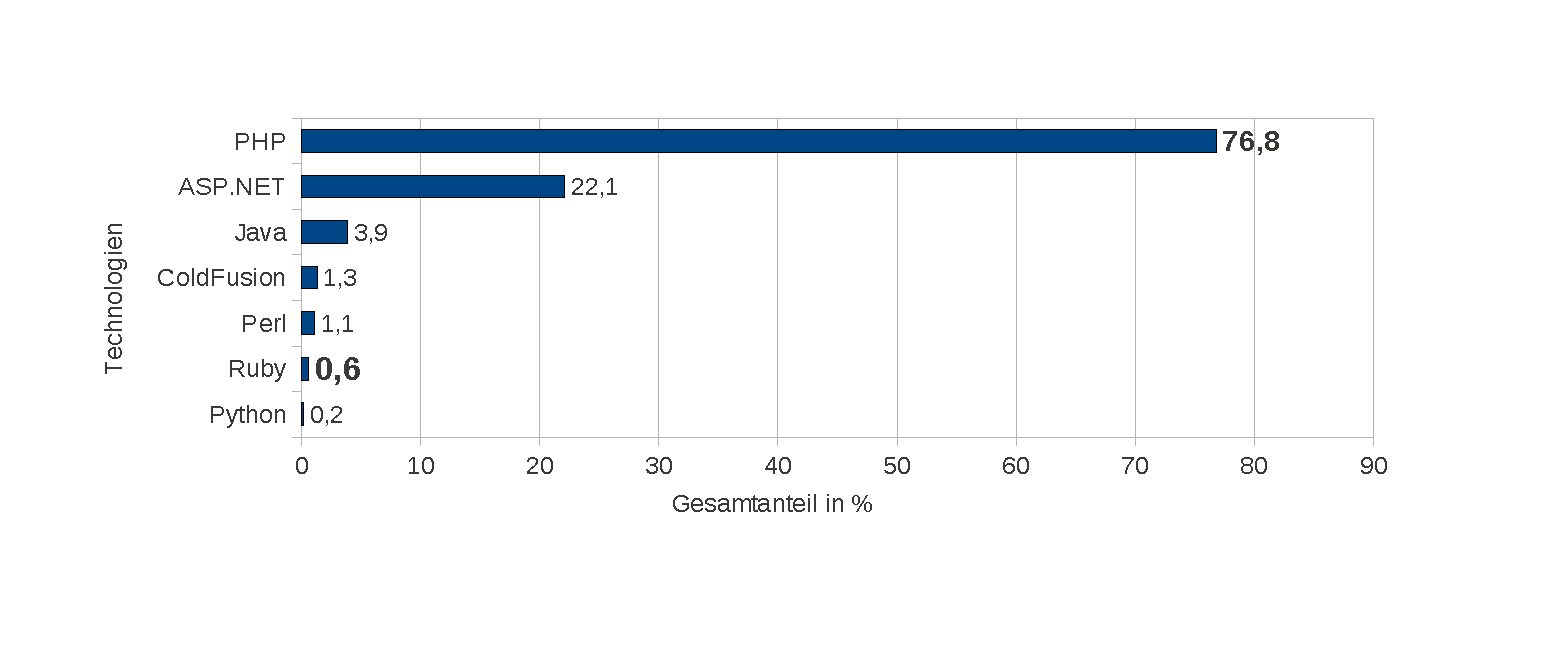
\includegraphics[scale=0.6]{images/Einleitung/serverseitigeScriptsprachen.pdf}
\caption[Nutzung verschiedener Programmiersprachen auf Servern]{Nutzung verschiedener Programmiersprachen auf Servern}{Quelle: Eigene Darstellung nach \citep{w3techs}}
\end{center}
\end{figure}

Auch im Bereich der Web Content Management Systeme\footnote{Im folgenden wird für den Begriff Web Content Management System(e) die Abkürzung WCMS verwendet.} spiegelt sich diese Dominanz wider. Betrachtet man die Angaben des Content Management Portals cmsmatrix.org\footnote{\href{http://cmsmatrix.org}{http://cmsmatrix.org} ermöglicht eine Gegenüberstellung der Funktionalitäten von Content Management Systemen unterschiedlicher Prgrammiersprachen.}, existieren neben den vor allem in Deutschland verwendeten Open Source-Lösungen Typo3, Drupal, Contao oder Joomla! über 500 weitere in PHP implementierte Web Content Management Systeme unterschiedlichster Ausprägung und Qualität.
Ruby als Programmiersprache findet hingegen nur bei etwa 1 Prozent der erfassten Server Verwendung. Die dabei umgesetzten Projekte sind jedoch meist individuelle, browser-basierte Applikationen, die für Unternehmen und deren spezifisches Geschäftsfeld entwickelt wurden. Bekannte Vertreter sind hier u.a. die webbasierte Projektmanagement-Applikation Basecamp von 37signals\footnote{Projektseite von Basecamp:\href{http://basecamphq.com}{ http://basecamphq.com/}}, der Microblogging-Dienst Twitter\footnote{
Großteile der Programmierung von Twitter basierten bis April 2011 auf dem Ruby on Rails Framework.} und der webbasierte Hosting-Dienst Github\footnote{Github greift neben Ruby on Rails noch auf andere Webframeworks und Technologiesysteme zurück.} für Software-Entwicklungsprojekte.
Diese individuellen Lösungen werden dabei meist unter Zuhilfenahme eines Web Application Framework realisiert, das den Entwicklungsprozess unterstützt und vereinfacht.
%\begin{}
%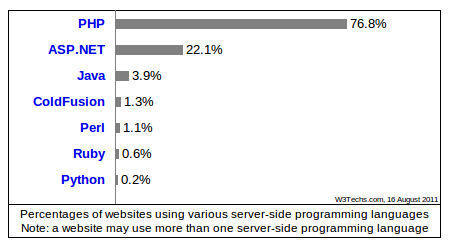
\includegraphics[width=\linewidth]{images/Einleitung/serverseitigeScriptsprachen.png}
%\caption{}
%\label{fig:beispiel}
%\end{figure}
\section{Motivation und Zielsetzung}
Ruby on Rails\footnote{Im weiteren Verlauf dieser Arbeit wird für das Webframework Ruby on Rails die Kurzform Rails verwendet.} hat sich seit der Veröffentlichung der Version 1.0 im Juli 2004 zu einem der bekanntesten Webframeworks der Ruby Fangemeinde entwickelt.
Startups\footnote{Der Begriff Startup bezeichnet hier junge Unternehmen, die sich mit ihrem neuartigen, meist innovativen Produkt noch nicht am Markt etabliert haben.} sowie etablierte Unternehmen greifen dabei verstärkt\footnote{Unter \href{http://rubyonrails.org/applications}{http://rubyonrails.org/applications} findet sich eine Übersicht ausgewählter Unternehmen, die auf Grundlage von Ruby on Rails teilweise gewinnerzielende Webanwendungen umgesetzt  haben. Die Entwicklungseinschätzung erfolgte an Hand der Community und dem Arbeitsmarktangebot, der eine zunehmende Nachfrage für Rails-Entwickler erkennen lässt.} auf das Rails Framework zurück, um ihre webbasierten Geschäftsideen und -modelle zu realisieren.
Wird neben der Webapplikation zusätzlich eine Internetseite zur Repräsentierung des Unternehmens benötigt, haben sich in der Praxis folgende zwei Lösungsansätze herausgebildet:

\begin{enumerate}
\item{
Bei geringem Umfang der zusätzlichen Internetseite werden die Inhalte manuell in HTML-Dateien angelegt und anschließend in die Rails-Anwendung integriert. Komfortable Möglichkeiten der Content-Verwaltung werden nicht angeboten oder später rudimentär nach implementiert. Änderungen der Inhalte sind teilweise mit erhöhtem Aufwand verbunden oder erfordern zusätzliche Programmierkenntnisse\footnote{Änderungen am Quellcode von Rails-Anwendungen im Produktivmodus erfordern immer einen Neustart des Servers.}.
}

\item{
Komplexe Internetseiten mit vielen Inhalten und anspruchsvollem Layout werden über ein Web Content Management System eines Drittanbieters realisiert. Die Rails-Anwendung fungiert als Zwischenstation und leitet bestimmte Anfragen an das externe WCMS weiter.
}
\end{enumerate}Während der erste Lösungsansatz bei wenigen Inhalten noch vertretbar ist, erfordert die Verwendung eines externen WCMS zusätzlichen Installations- und Wartungsaufwand. Weiterhin erhöht sich der Bedarf an Programmierern, da neben Ruby nun auch andere Programmiersprachen (die des externen WCMS) Verwendung finden können.
\newline
\newline
Ziel der vorliegende Arbeit ist es daher, die Möglichkeiten einer komplett rails-basierten Web Content Management Verwaltung zu untersuchen, um so den Einsatz eines externen WCMS überflüssig werden zu lassen.
\newline
\newline
Dafür werden unter Verwendung der vergleichenden Methode die ausgewählten Ruby on Rails Content Management Systeme Alchemy CMS, Browser CMS, Locomotive CMS und Refinery CMS einem externen Kriterienkatalog gegenübergestellt, der allgemein gültige Anforderungen an Web Content Management Systeme formuliert. An Hand der Ergebnisse des Vergleichs kann abschließend eine Leistungsbeurteilung für die gewählten Systeme erfolgen, in wie weit sich diese für den Einsatz im Bereich des Web-Publishing eignen.
Zusätzlich wird auf nichtfunktionale Aspekte bei der Umsetzung der Systeme eingegangen und auf mögliche Probleme hingewiesen.

\section{Aufbau der Arbeit}
Die vorliegende Diplomarbeit gliedert sich in sechs Abschnitte:
\newline
\newline
In Kapitel 2 werden die für die funktionelle und programmiertechnische Analyse der Systeme notwendigen theoretischen Grundlagen zu Web Content Management Systemen und dem Ruby on Rails Webframework geschaffen.
Darüber hinaus wird der für die Ermittlung der Leistungsfähigkeit der Systeme verwendete Kriterienkatalog vorgestellt.
\newline
\newline
In Kapitel 3 folgt die funktionale Analyse der ausgewählten Ruby on Rails 3 Web Content Management Systeme Alchemy CMS, Refinery CMS, Browser CMS und Lokomotive CMS. Dazu werden die Kriterien des im Kapitel 2 vorgestellten Katalogs mit den tatsächlich gebotenen Funktionalitäten der gewählten WCMS verglichen. Die Untersuchung schließt mit einer Zusammenfassung der Ergebnisse und einer Einschätzung für den Einsatz der WCMS ab.\\
\newline
Kapitel 4 überprüft die analysierten WCM-Systeme auf vorhandene konzeptionelle und programmiertechnische Schwachstellen.
Darauf aufbauend werden in Kapitel 5 mögliche Lösungsansätze demonstriert und die dafür notwendigen theoretischen Grundlagen herausgearbeitet.
Kapitel 6 schließt die Arbeit mit einer Zusammenfassung der herausgearbeiteten Ergebnisse ab und gibt Ausblicke auf zukünftige Entwicklungspotenziale.
%
% EOF
%


\chapter{Grundlagen}

\section{Entwicklung mit Ruby on Rails}

2004 arbeitete der dänische Programmierer David Heinemeier Hansson an der Umsetzung eines webbasierten Projektmanagement-Tools mit dem Namen Basecamp\footnote{Projekt-Homepage: \href{http://basecamphq.com/}{http://basecamphq.com/}}. Die bei der Realisierung des Projektes umgesetzten Teilkomponenten extrahierte er später und veröffentlicht sie 2005 als Framework unter dem Namen Ruby on Rails.
Ruby on Rails basiert dabei auf der objektorientierten Programmiersprache Ruby und ermöglicht die schnelle Entwicklung von Webanwendungen nach dem MVC-Paradigma (Kapitel sec:mvc).
\newline
6 Jahre später (die zahlreiche Änderungen und Verbesserungen am Framework ermöglichten) beschreibt sich das Ruby on Rails-Projekt selbst mit folgenden plakativen Worten:
\begin{quote}
Ruby on Rails is an open-source web framework that’s
optimized for programmer happiness and sustainable
productivity. It lets you write beautiful code by
favoring convention over configuration. \cite[vgl.][]{RailsStatement}
\end{quote}

Diese subjektive Aussage der Rails-Kernentwickler bezieht sich dabei auf viele Ansätze und Entwicklungsabläufe, die innerhalb des Frameworks umgesetzt werden.
Im folgenden Abschnitt sollen die mit dieser Aussage angedeuteten wichtigsten Prinzipien, Paradigmen und Programmierabläufe des Frameworks zusammengefasst werden, um auf dieser Grundlage eine nichtfunktionale Betrachtung der Rails WCMS in Kapitel 4 zu ermöglichen. Auf die Themen Rest (Kapitel \ref{grundrest}) und Middleware (Kapitel \ref{grundrack}) wird dabei ausführlicher eingegangen, um für die in Kapitel 5 umgesetzten Lösungsvorschläge entsprechendes Vorwissen zu schaffen.
\newline
\newline
Für eine umfassende Einführung in Rails werden \cite{RubyMetaprogramming2010} und \cite{EnterpriseRails} empfohlen.

\subsection{Don't-Repeat-Yourself (DRY)}
Zur Optimierung der Entwicklungvorgänge innerhalb des Frameworks propagiert Rails den Grundsatz des DRY (Don't-Repeat-Yourself). Dabei sollen Redundanzen, d.h. die wiederholte Angabe identischer Informationen jeglicher Art vermieden werden. So kann sichergestellt werden, dass sich Änderungen an einer zentralen Stelle im System (z.B. Quellcode) in der gesamten Anwendung auswirken und Duplikate nicht mehrfach angepasst werden müssen.
\subsection{Convention over Configuration}
Viele Web Frameworks müssen vor ihrer Nutzung erst mit Hilfe zahlreicher Konfigurationsdateien und Parametereinstellungen zu einem lauffähigen Gesamtsystem zusammengebaut werden\footnote{Rails bezeichnet diese Art der Frameworks mit ihrem Konfigurations-Overhead oft als \emph{enterprisy}. Dies bedeutet jedoch nicht, das Rails für Anwendungsumsetzungen im Enterprise-Bereich ungeeignet ist. \citep[vgl.][]{enterprisy}.}. Abbildung \ref{spring} zeigt beispielhaft solch eine Konfigurationsdatei innerhalb des Java Application Frameworks Spring\footnote{Projektseite: \href{http://www.springsource.org/}{http://www.springsource.org/}}:

\lstinputlisting[label=spring,language=xml, caption=Konfigurationsdatei im Java Spring Framework]{code/spring.xml}
Um diesen zusätzlichen und zeitraubenden Aufwand vor der eigentlichen Arbeit mit einem Framework zu vermeiden, definiert Rails zahlreiche Konventionen, die es erlauben, sofort mit der Entwicklungsarbeit zu beginnen. U.a. werden folgende Festlegungen getroffen:

\begin{itemize}
\item
Informationen zur Datenbankverbindung der Anwendung müssen in der Datei database.yml im Unterordner config hinterlegt werden
\item
Der Klassenname eines Domainenmodells wird im Singular erwartet, der dazu korrespondierende Tabellename in der Datenbank hingegen im Plural z.B. Domainenmodell Project => Datenbanktabelle projects
\item
Der Primärschlüssel in einer Datanbanktabelle muss vom Typ Integer sein und den Namen ID besitzen
\item
Rails erwartet eine definierte Ordnerstrukur für Controller, Domainmodell und Views\footnote{Eine Erklärung zu Model-View-Controller folgt in Abschnitt \ref{sec:mvc}}
\end{itemize}
Für den produktiven Einsatz des Frameworks müssen diese daher erlernt und akzeptiert werden, was dazu führt, dass Rails häufig als \emph{opinionated software\footnote{Eine ausführliche Stellungnahme von Rails-Erfinder David Heinemeier Hansson zu diesem Thema gibt es unter: \href{http://www.linuxjournal.com/article/8686}{http://www.linuxjournal.com/article/8686}}} (starr- und eigensinnige Software) bezeichnet wird.

Ein Abweichen von den definierten Konventionen ist jederzeit möglich, erhöht jedoch den Aufwand des Entwicklers.

\subsection{Model-View-Controller (MVC)}
\label{sec:mvc}
Für Software-Designer ist es  eine gebräuchliche Technik, komplexe Software-Systeme durch Schichtenbildung in einzelne Bestandteile zu zerlegen \citep[Kapitel 1]{FowlerPatterns}. Das Ruby on Rails Framework baut ebenfalls auf einem Mehr-Schichten-Architektur-Modell auf. Zusätzlich kommt eine für das Rails-Framework spezifische Implementierung des bereits 1979 von dem Norweger Trygve Mikkjel Heyerdahl entwickelten Model-View-Controller-Paradigmas zum Einsatz\footnote{In der Fachliteratur wird das MVC-Paradigma häufig auf die Schichtenarchitektur einer Anwendung übertragen \cite[S. 544 ff.]{objekt}. Tatsächlich betrifft MVC in seiner  ursprünglichen Form nur die Präsentationsschicht einer Webanwendung.}.
Abbildung \ref{fig:mvcimage} charakterisiert den Ablauf einer Anfrage (Request) an eine Rails-Anwendung innerhalb des Client-Server-Modells sowie die Komponenten Model, View und Controller, die eine exakte Trennung der Verantwortungsbereiche in einer Rails-Anwendung sicherstellen:

\begin{figure}[!h]
\begin{center}
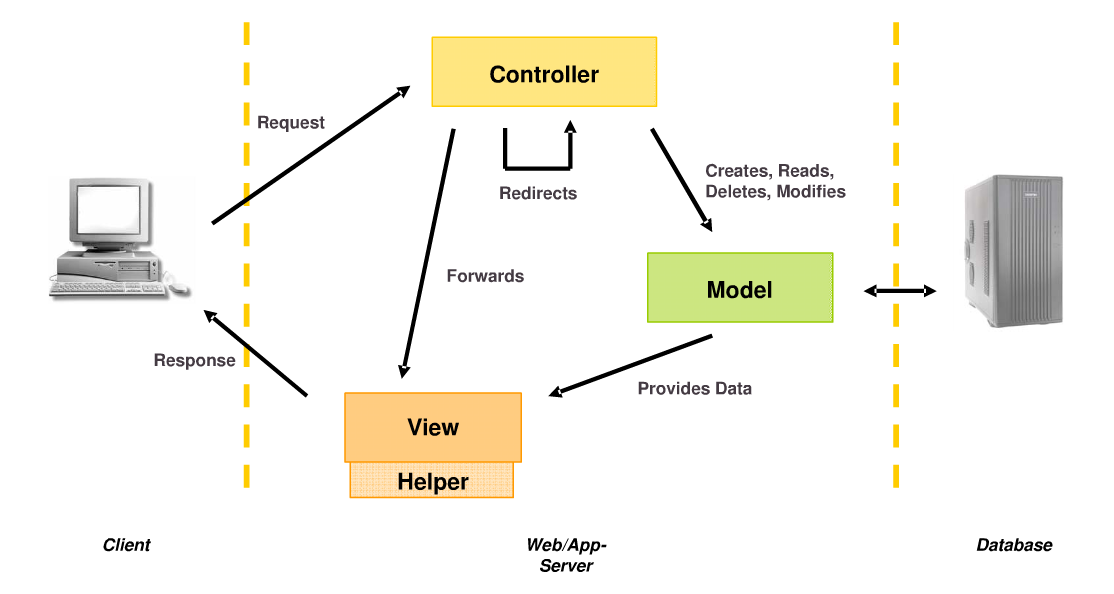
\includegraphics[scale=0.4]{images/analyse/mvc.png}
%\caption{Nutzung verschiedener Programmiersprachen auf Servern}{Quelle: \citep{w3techs}}


\caption[Verarbeitung einer Anfrage innerhalb des Rails-Frameworks]{Verarbeitung einer Anfrage (Client-Server-Modell) innerhalb des Rails-Frameworks. Quelle: \citep[Seite 6]{railsmvc}}
\label{fig:mvcimage}
\end{center}
\end{figure}

\begin{enumerate}
\item
Anfrage eines Clienten
\item
An Hand der im Rails-Routing definierten Einträge wird die Anfrage eines Clienten an den registrierten Controller weitergeleitet
\item
Der Controller steuert den Ablauf innerhalb der Anwendung. Dabei greift er über ein Model auf benötigte Daten in einem Speicher (z.B. relationale Datenbank) zu und stellt diese dem View-Layer zur Verfügung. Es ist auch möglich, dass der Controller die Anfrage an einen anderen Controller weiterleitet (Redirects). Im Gesamtkonzept von Rails enthält der Controller die Programmlogik der Anwendung.
\item
Als Model werden in Rails Ruby-Klassen bezeichnet, die einen Zugriff auf relationale Datenbanken oder andere Datenspeicher ermöglichen \citep[vgl.][]{Rails2}. Es bildet innerhalb der Anwendung die zugrundliegende Datenstruktur ab.
%\citep[vgl.][]{Rails2}
\item
Der View-Layer (Sicht- oder Darstellungsschicht) bereitet die durch den Controller zur Verfügung gestellten Daten in der angeforderten Darstellungsform auf und gibt das Ergebnis der Anfrage aus. So wird je nach spezifiziertem Format z.B. eine HTML- oder XML-Datei erzeugt. Ein View repräsentiert somit die Darstellung einer bestimmten Datenstruktur (Model).
\item
Das Ergebnis der Anfrage (die Ausgabe des View) wird vom Framework an den Server übermittelt und von dort an den Clienten ausgeliefert (Response). Der Kommunikationsprozess mit dem Rails-Framework ist damit abgeschlossen.
\end{enumerate}



\subsection{REST}
\label{grundrest}
Innerhalb einer Web-Applikation erfolgt der Austausch zwischen Server und Client durch die Nutzung des HTTP-Protokolls. Dabei wird eine Anfrage (Request) an einen Server geschickt, bearbeitet und eine entsprechende Antwort (Response) mit den angeforderten Inhalten zurückliefert. Ein Großteil der Webanwendungen interpretiert dabei die im HTTP-Protokoll definierten Methoden GET und POST:

\begin{description}
\item[GET]
Anforderung an den Server, eine über die Adresszeile des Browsers angegebene Ressource zurückzuliefern. Es können zusätzlich Argumente an die angeforderte URL angehängt werden.
\item[POST]
Mit Hilfe dieser Methode ist es möglich, große Datenmengen aus z.B. Formularen an einen Webserver zu verschicken. Die übergebenen Informationen werden dabei im sogenannten Body der Anfrage codiert mitverschickt und somit im Vergleich zu GET nicht in der URL sichtbar\footnote{Ein Post-Request findet vor allem bei der Übermittlung von Formularen innerhalb eines Browsers Verwendung.}.
\end{description}


REST, ein Akronym für \textbf{RE}epresentational \textbf{S}tate \textbf{T}ransfer, erweitert die in  traditionellen Webanwendungen üblichen GET und POST um die ebenfalls im HTTP-Standard enthaltenen Methoden PUT und DELETE:
\begin{comment}
\begin{description}
\item[GET]
Abfrage einer Ressource unter der angegebenen URL mit  anschließender Darstellung
\item[POST]
Erstellung einer neuen Ressourcen an Hand der in der Anfrage übermittelten Daten, Realisierung durch Formulare auf Clientseite
\item[PUT]
Überschreiben der angeforderten Ressource mit den in der Anfrage neu übermittelten Daten
\item[DELETE]
Löschen der beschriebenen Ressource
\end{description}
\end{comment}

\begin{description}
\item[PUT]
	Die Verwendung der PUT-Methode zeigt die Neuanlage der in einer	Anfrage spezifizierten Ressource an
\item[DELETE]
	Die Verwendung dieser Methode signalisiert dem Server, die angegebene Ressource auf dem Server zu löschen.
\end{description}
Da aktuelle Browser nur GET- und POST-Anfragen zuverlässig unterstützen, müssen entsprechende Anfragen zum Löschen und Verändern einer Ressource mit Hilfe von zusätzlichen Attributen in der Anfrage simuliert werden\footnote{Das Rails Framework fügt  innerhalb von Formularen automatisch einen versteckten Parameter \emph{\_method} in die Anfrage, die den Namen der gewünschten HTTP-Metode (DELETE oder PUT) enthält. Im Framework wird dieser Parameter ausgelesen und ein entsprechendes Routing zur geforderten Controller-Action eingeleitet.}. Das folgende Beispiel stellt das von Rails definierte Standard-Routing einer als \emph{restful} angelegten Ressource Projekt dar\footnote{REST wird nicht über einen entsprechend formulierten Standard definiert. Vielmehr kann es als Programmierparadigma innerhalb von Web-Anwendungen verstanden werden, die eine Ansammlung von Best-Practices darstellen \cite{restful}.}.

\begin{table}[!h]
\caption{Rails Routing der Rest-Ressource Projekt}
\center
\begin{tabular}[!ht]{|p{2cm}|p{3cm}|p{3cm}|p{6cm}|}
\hline
HTTP-Methode & Anfragepfad & Ausgelöste Aktion im Controller & Wirkung\\
\hline
GET	& /projects & index & Anzeige aller vorhandenen Projekte\\
\hline
GET	& /projects/new	& new &	Anzeige eines HTML-Formulars zum erstellen eines neuen Projektes\\
\hline
POST & /projects & create & Erstellt ein neues Projekt mit den übermittelten Daten\\
\hline
GET & /projects/:id &	show &	Anzeige eines Projektes mit der zugeordneten ID\\
\hline
GET	& /projects/:id/edit & edit & Anzeige eines HTML-Formulars zum Bearbeiten eines bestehenden Projektes\\
\hline
PUT	& /projects/:id &	update & Aktualisierung eines bestimmten Projektes mit den übermittelten Daten\\
\hline
DELETE & /projects/:id &	destroy &	Löschung des Projektes mit der angegebenen ID\\
\hline
\end{tabular}
\end{table}

\begin{table}[!ht]
\caption{Vergleich zwischen Rest-konformen und klassischen Rails-URL's}
\label{tab.restnonrest}
\center
\begin{tabular}[!ht]{|l|l|l|}
\hline
Aktion & normale URL & 	REST URL in Rails \\
\hline
show &	/projects/show/12 &	/projects/12 \\
\hline
delete & /projects/destroy/123 & /projects/123 \\
\hline
update & /projects/update/123 &	/projects/123 \\
\hline
create & /projects/create & /projects \\
\hline
\end{tabular}
\end{table}

Tabelle \ref{tab.restnonrest} zeigt noch einmal die Trennung zwischen Ressource und Aktion innerhalb einer in Rails definierten REST-Ressource Projekt. Eine ausführliche Beschreibung von REST und dessen Realisierung liefert \cite{restful}.

\newpage
\subsection{Rack und Middleware}
\label{grundrack}
Rails ist innerhalb der Ruby-Gemeinde nicht das einzigste existierende Webframework. Mit den Projekten Sinatra\footnote{Projektseite: \href{http://www.sinatrarb.com/}{http://www.sinatrarb.com/}}, Merb\footnote{Projektseite: \href{http://www.merbivore.com/}{http://www.merbivore.com/}}, Camping\footnote{Projektseite: \href{http://camping.rubyforge.org/}{http://camping.rubyforge.org/}} und Ramaze\footnote{Projektseite: \href{http://ramaze.net/}{http://ramaze.net/}} stehen weitere Alternativen mit unterschiedlichen Ansätzen und Funktionsumfängen zur Verfügung.
Bei der Implementierung dieser Frameworks müssen Entwickler wiederholt Adapter\footnote{} (Handler) zur Ansteuerung verschiedener Webserver entwickeln. Durch Rack\footnote{Projektseite: \href{http://rack.rubyforge.org/}{http://rack.rubyforge.org/}}, einem Ruby Webserver Interface, lässt sich die wiederholte Implementierung solcher Adapter in den einzelnen Frameworks vermeiden.
\begin{figure}[!h]
\begin{center}
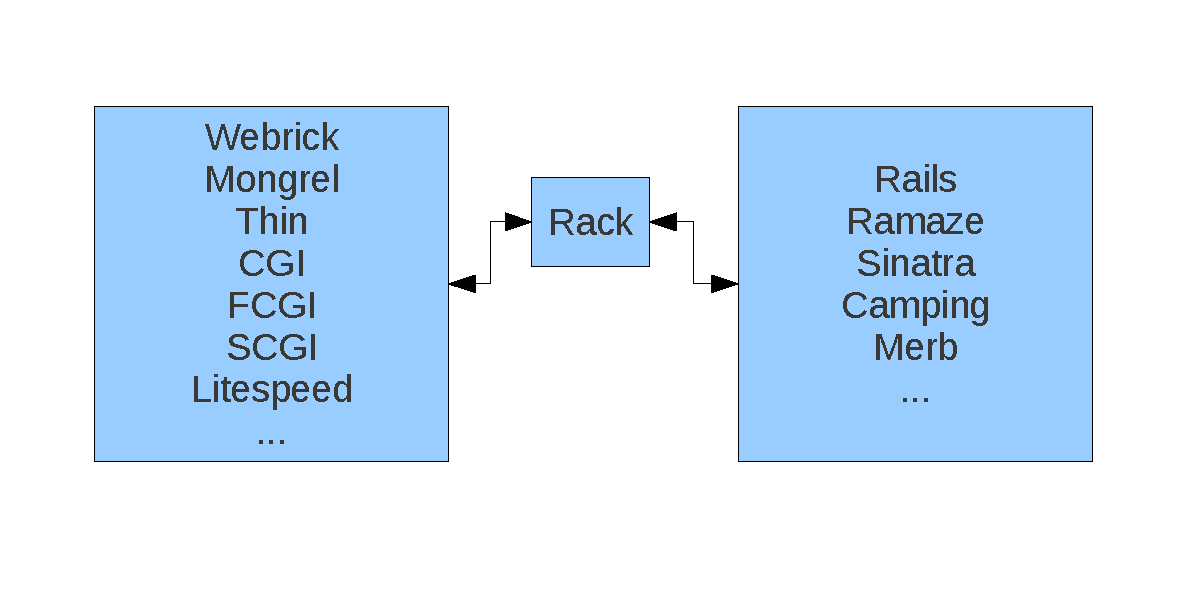
\includegraphics[scale=0.6]{images/rack/rack.pdf}
\caption{Rack als Vermittler zwischen Server und Ruby-Webframeworks}
\label{rackschema}
\end{center}
\end{figure}


Damit Server und Frameworks untereinander kommunizieren können, muss eine Rack-Anwendung bestimmte Methoden implementieren und ein bestimmtes Rückgabeformat einhalten. An Hand des Beispiels in \ref{rack} sollen diese formalen Kriterien beschrieben werden:

\lstinputlisting[label=rack,language=Ruby, caption=Beispiel für eine einfache Rack-Anwendung]{code/rack.rb}

\begin{description}
\item[Zeile 6-8]\mbox{~}\\*
Initialisierung der Rack-Anwendung MyRackApp unter Angabe eines zuvor übergebenen Namen (\emph{Rack} in Zeile 15).
\item[Zeile 10-12]\mbox{~}\\*
Implementierung der für eine Rack-Anwendung notwendigen Methode \emph{call}. Diese wird vom Webserver beim Start einer Anfrage aufgerufen und muss als Antwort (Rückgabewert) einen Ruby-Hash mit den folgenden Informationen zurückliefern:
\begin{description}
\item[Status]\mbox{~}\\*
Angabe des HTTP-Statuscode, \emph{200} bedeutet in diesem Beispiel eine erfolgreiche Ausführung der Anfrage am Server\footnote{Die HTTP-Statuscodes sind im HTTP-Protokoll definiert und können u.a. unter folgender Quelle eingesehen werden: \href{http://www.w3.org/Protocols/rfc2616/rfc2616-sec10.html}{http://www.w3.org/Protocols/rfc2616/rfc2616-sec10.html}}
\item[Header]\mbox{~}\\*
Angabe von im HTTP-Protokoll definierten Header-Informationen,  im Beispiel wird ein einfaches Textdokument (\emph{text/plain}) zurückgeliefert
\item[Response]\mbox{~}\\*
Die Antwort der Rack-Anwendung, im Beispiel wird ein String \emph{Hello Rack!} an den Server übergeben und von diesem ausgeliefert.
\end{description}

Beim Aufruf der Methode \emph{call} (Zeile 15) übergibt der Server eine Variable \emph{env}, die alle wichtigen Informationen über die Serverumgebung und Anfrageparameter enthält.
\item[Zeile 15]\mbox{~}\\*
Start des Mongrel Webservers und Initialisierung der Rack-Anwendung \emph{MyRackApp}.
\end{description}

Bei einem Aufruf der Adresse \emph{localhost:3001} in einem Browser wird vom gestarteten Mongrel-Server der Rückgabewert der Methode \emph{call} ausgegeben (Abb. \ref{rackoutput}).

\begin{figure}[!ht]
\begin{center}
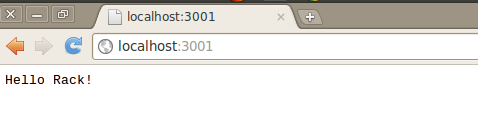
\includegraphics[scale=0.6]{images/rack/outputrack2.png}
\caption{Ausgabe der Rack-Anwendung MyRackApp im Browser}
\label{rackoutput}
\end{center}
\end{figure}

Durch die Nutzung von Rack ergeben sich im Bereich der Ruby Webframeworks folgende Vorteile:

\begin{itemize}
\item
Vereinfachung der Webframework-Entwicklung: Ein Framework, das Rack unterstützt, kann sofort von allen anderen rack-unterstützenden Webservern verwendet werden.
\item
Vereinfachung der Serverentwicklung: Ein rack-unterstützender Server kann sofort mit allen rack-basierten Webframeworks eingesetzt werden.
\item
Keine Codeduplizierung durch wiederholte Entwicklung von Server-Adaptern innerhalb der verschiedenen Ruby Webframeworks
\item
Rack beinhaltet Handler für die meist verbreitesten Webserver in Ruby (Abbildung \ref{rackschema})
\end{itemize}


Darüber hinaus ist es  möglich, einzelne Rack-Anwendungen hintereinander zu schalten und so ein Filtersystem für ankommende Anfragen und ausgehende Antworten vor dem eigentlichen Webframework zu realisieren.
Diese Anwendungen werden Rack-Middlewares genannt und können in einer Rails-Anwendung in der Startkonfiguration des Frameworks eingebunden werden. So kann das Ein- und Ausgabeverhalten des Railsframeworks gezielt verändert werden, da die einzelnen Rack-Anwendungen entscheiden, ob der nächste Filter (die nächste registrierte Rack-Middleware) oder eine vorzeitige Anwort an den Server geschickt werden soll.

%\lstinputlisting[label=middlewarestack,language=Ruby, caption=Registrierung verschiedener Middlewares in einer Rails 3 Anwendung]{code/middleware.rb}
Das Rails-Framework steht selbst am Ende der Filterliste und ist im Kontext von Rack selbst als Rack-Anwendung eingebunden (Abb. \ref{rackmiddlewares}).
\begin{figure}[!ht]
\begin{center}
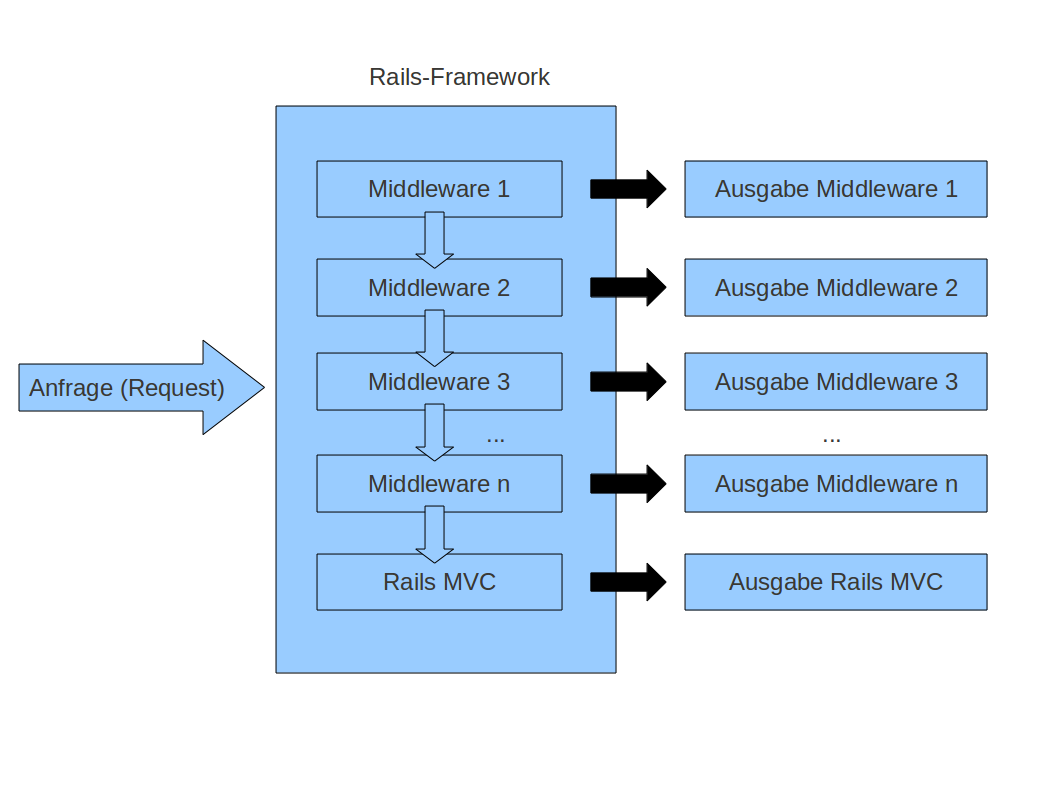
\includegraphics[scale=0.5]{images/rack/middlewares.png}
\caption{Möglichkeiten der unterschiedlichen Rückgabewerte durch Rack Middlewares und Rails}
\label{rackmiddlewares}
\end{center}
\end{figure}
Eine detaillierte Beschreibung von Rack und der Einrichtung eines komplexen Filtersystems\footnote{Rack stellt häufig verwendete Middlewares für verschiedene Aufgabenbereiche zur Verfügung. Die Projektseite ist unter folgender Adresse verfügbar: \href{https://github.com/rack/rack-contrib}{https://github.com/rack/rack-contrib}} in einer Rails-Anwendung liefern \cite{rack} und \cite{railsguiderack}.

\subsection{Generatoren}
\label{sec:railsgeneratoren}
Das Ruby on Rails Framework unterstützt mit Hilfe sogenannter Generatorskripte die automatische Erzeugung von funktionsfähigem Quellcode. Der folgende Scaffold-Generator\footnote{Scaffold kann in diesem Zusammenhang mit dem Wort Grundgerüst übersetzt werden.} erstellt z.B. nach dessen Initialisierung ein komplett funktionsbereites Codegerüst für die in Rails benötigten MVC-Komponenten einer Ressource \emph{Projekt}.

\begin{lstlisting}[caption=Aufruf des Generators zur Erstellung einer MVC-Ressource Projekt]
rails g scaffold project name:string description:text
\end{lstlisting}

\lstinputlisting[label=scaffold,language=Ruby, caption=Auflistung der erstellten Dateien des Scaffold-Generators]{code/scaffold.txt}

\section{Web Content Management, Content Life Cycle und Web-Publishing}
\label{sec:webpublishing}
Der in der einschlägigen Literatur bereits mehrfach thematisierte Anstieg von Content\footnote{
\glqq Unter dem Begriff des \flqq Contents\frqq~ werden alle Inhalte verstanden, die in einem CMS verwaltet werden und die im engeren Sinne für die Erstellung von Dokumenten und Publikationen verwendet werden. Darunter fallen alle textuellen und (audio-)visuellen Informationen [..] \citep[S. 297]{TechnischeDok}
} erfordert innerhalb der einzelnen Unternehmen ein immer umfangreicheres und zielgerichteteres Management. Der so entstandene Begriff des Content Management wird dabei u.a. von Berechtenbreiter mit folgenden Worten umschrieben:
\begin{quote}
Content Management beschreibt die Planung, Verwaltung, Steuerung und Koordination aller Aktivitäten, die auf den Content und dessen Präsentation in Unternehmen abstellen \cite{Berchtenbreiter}.
\end{quote}

Im Bereich der internet-basierten Web-Sites und Internet-Portale hat dies zur Herausbildung des Web Content Managements geführt \citep[][S. 3]{ecm}. Die dort verwendeten Softwarelösungen (WCMS) streben dabei die Implementierung des Content Life Cycle (Inhaltslebenszyklus) ab, der als stark vereinfachtes Prozessmodell alle wichtige Phasen\footnote{Die Content-Nutzung durch den Endanwender (Internetseitennutzer) findet innerhalb des Content Life Cycle keine Beachtung.}, die ein beliebiger Inhalt (Informationsträger) während seiner Existenz durchläuft, abbildet \citep[S.303]{TechnischeDok}. Im folgenden sollen diese Teilprozesse erläutert werden:

\begin{figure}[!ht]
\begin{center}
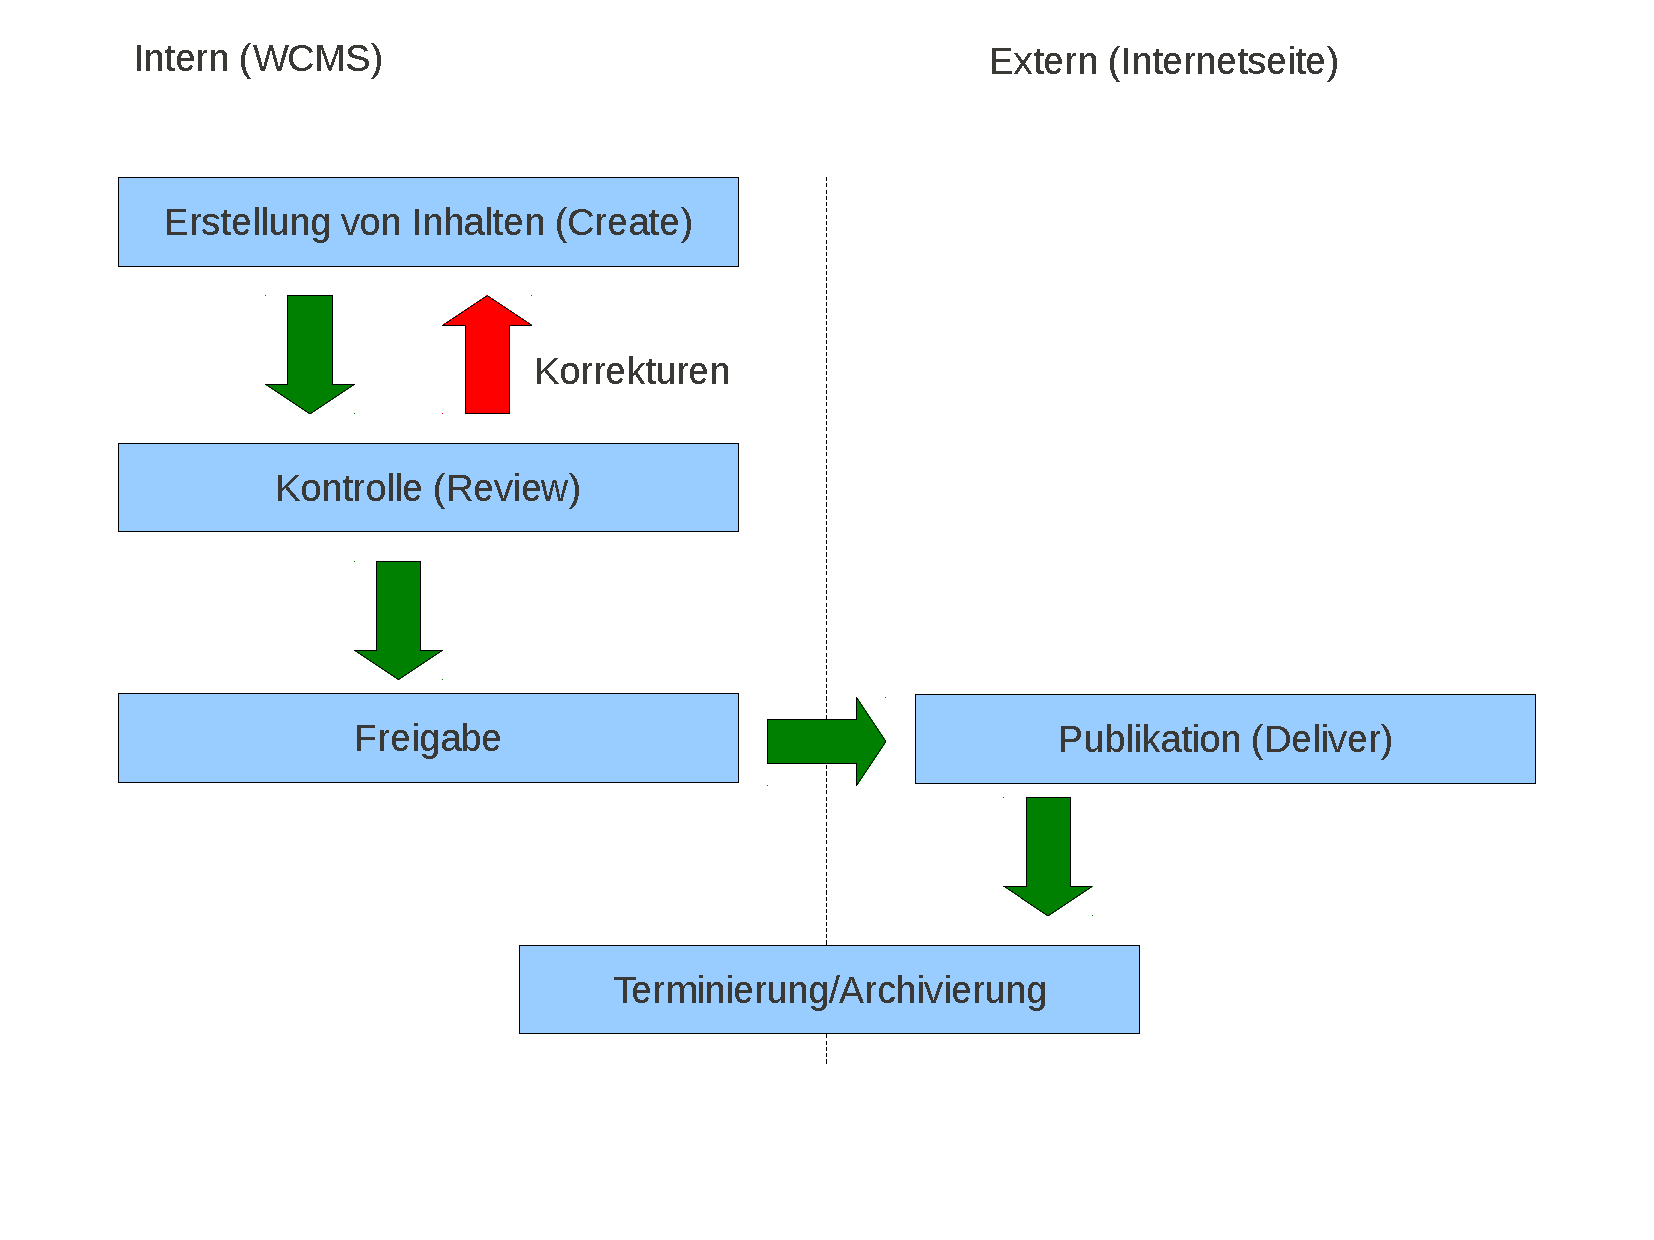
\includegraphics[scale=0.5]{images/grundlagen/lifecycle.pdf}
\caption[Prozessschritte im Content Life Cycle]{Prozessschritte im Content Life Cycle. Eigene Darstellung nach \citep[S. 81]{rockley} und \citep[S. 10]{RitterSwot}}
\label{rackmiddlewares}
\end{center}
\end{figure}


\begin{description}
\item[Erstellung]\mbox{~}\\*
Autoren oder Benutzer erzeugen die Inhalte einer Internetseite an Hand der vorliegenden digitalen, (audio-)visuellen Medien oder anderer Informationsträger.
\item[Freigabe und Kontrolle]\mbox{~}\\*
Die Kontrolle von Content schließt sich dem Teilprozess der Content-Erstellung an und stellt durch verschiedene Redakteure und Arbeitsabläufe (Workflows) die Qualität der Inhalte, die auf der Internetseite veröffentlicht werden sollen, sicher. Die Komplexität der Kontrollinstanzen kann dabei unterschiedlich ausgeprägt sein und muss den tatsächlichen Gegebenheiten angepasst werden. Erfüllt der Content die inhaltlichen und gestalterischen Anforderungen nicht, muss dieser von den Autoren erneut überarbeitet werden.
\item[Publikation]\mbox{~}\\*
Nach erfolgter Freigabe des Content erfolgt im Teilprozess Publikation die Veröffentlichung auf der Internetseite. Damit werden die bis dato ausschließlich internen Informationen externen Nutzern zugänglich gemacht. Die eingesetzten WCMS unterscheiden dabei häufig zwischen eine Inter-, Intra- oder Extranetveröffentlichung, welche die Erreichbarkeit der Inhalte auf bestimmte  Zielgruppen einschränkt.
\item[Terminierung und Archivierung]\mbox{~}\\*
Nach Verwendung des Content auf der Internetseite werden bestimmte Inhalte mit steigendem Alter uninteressant oder überflüssig (abhängig von der Art des Inhalts). Durch Aufnahme in ein internes oder öffentliches Archiv können diese für eine spätere Nutzung bzw. Wiederverwendung aufbewahrt werden.
\end{description}

Am Ende des Content Life Cycles kann somit die beabsichtigte Veröffentlichung der Internetinhalte realisiert werden. Somit trägt dass Modell des Content Life Cycle gleichzeitig zur Erfüllung des Web-Publishing-Begriffs bei, der
Der im folgenden Abschnitt vorgestellte Kriterienkatalog (zur funktionalen Analyse der WCMS) wird dabei in die Teilprozesse
 des Content Life Cycle aufgeteilt.\newpage

\section{Kriterienkatalog}
Die hohe Zahl am Markt befindlicher Web Content Management Systeme führt zu einem erschwerten Auswahlverfahren. Neben kommerziellen WCMS-Lösungen stehen durch die Open Source Bewegung zusätzlich zahlreiche kostenlose Softwareprodukte zur Verfügung, die sich in ihrer Leistungsfähigkeit stark unterscheiden.
So kommt es häufig vor, das klein angelegte Open Source Projekte ihre Software stolz als Web Content Management System bezeichnen, obwohl nur sehr wenige Funktionalitäten implementiert sind.
Um dieser Praktik entgegenzuwirken, haben Vertreter der Content Management Branche eine Feature-Matrix (Abb. \ref{featurematrix}) herausgegeben, die aktuelle Anforderungen an ein Content Management System spezifizieren soll. Die dabei entstandene Übersicht zeigt dabei eine Unterscheidung in 3 Prioritätsstufen:
\begin{description}
\item[Must-Have]\mbox{~}\\*
Diese Funktionalität muss in einem Web Content Management System verhanden sein.
\item[Should-Have]\mbox{~}\\*
Diese Funktionalität ist nicht zwingend notwendig, kann bei entsprechender Existenz aber sehr positv wahrgenommen werden.
\item[Nice-to-Have]\mbox{~}\\*
Funktionalitäten, die nur in wenigen, hochwertigen Systemen zur Verfügung stehen und über die gewöhnlichen Anforderungen hinausgehen.
\end{description}


\begin{figure}[!h]
\begin{center}
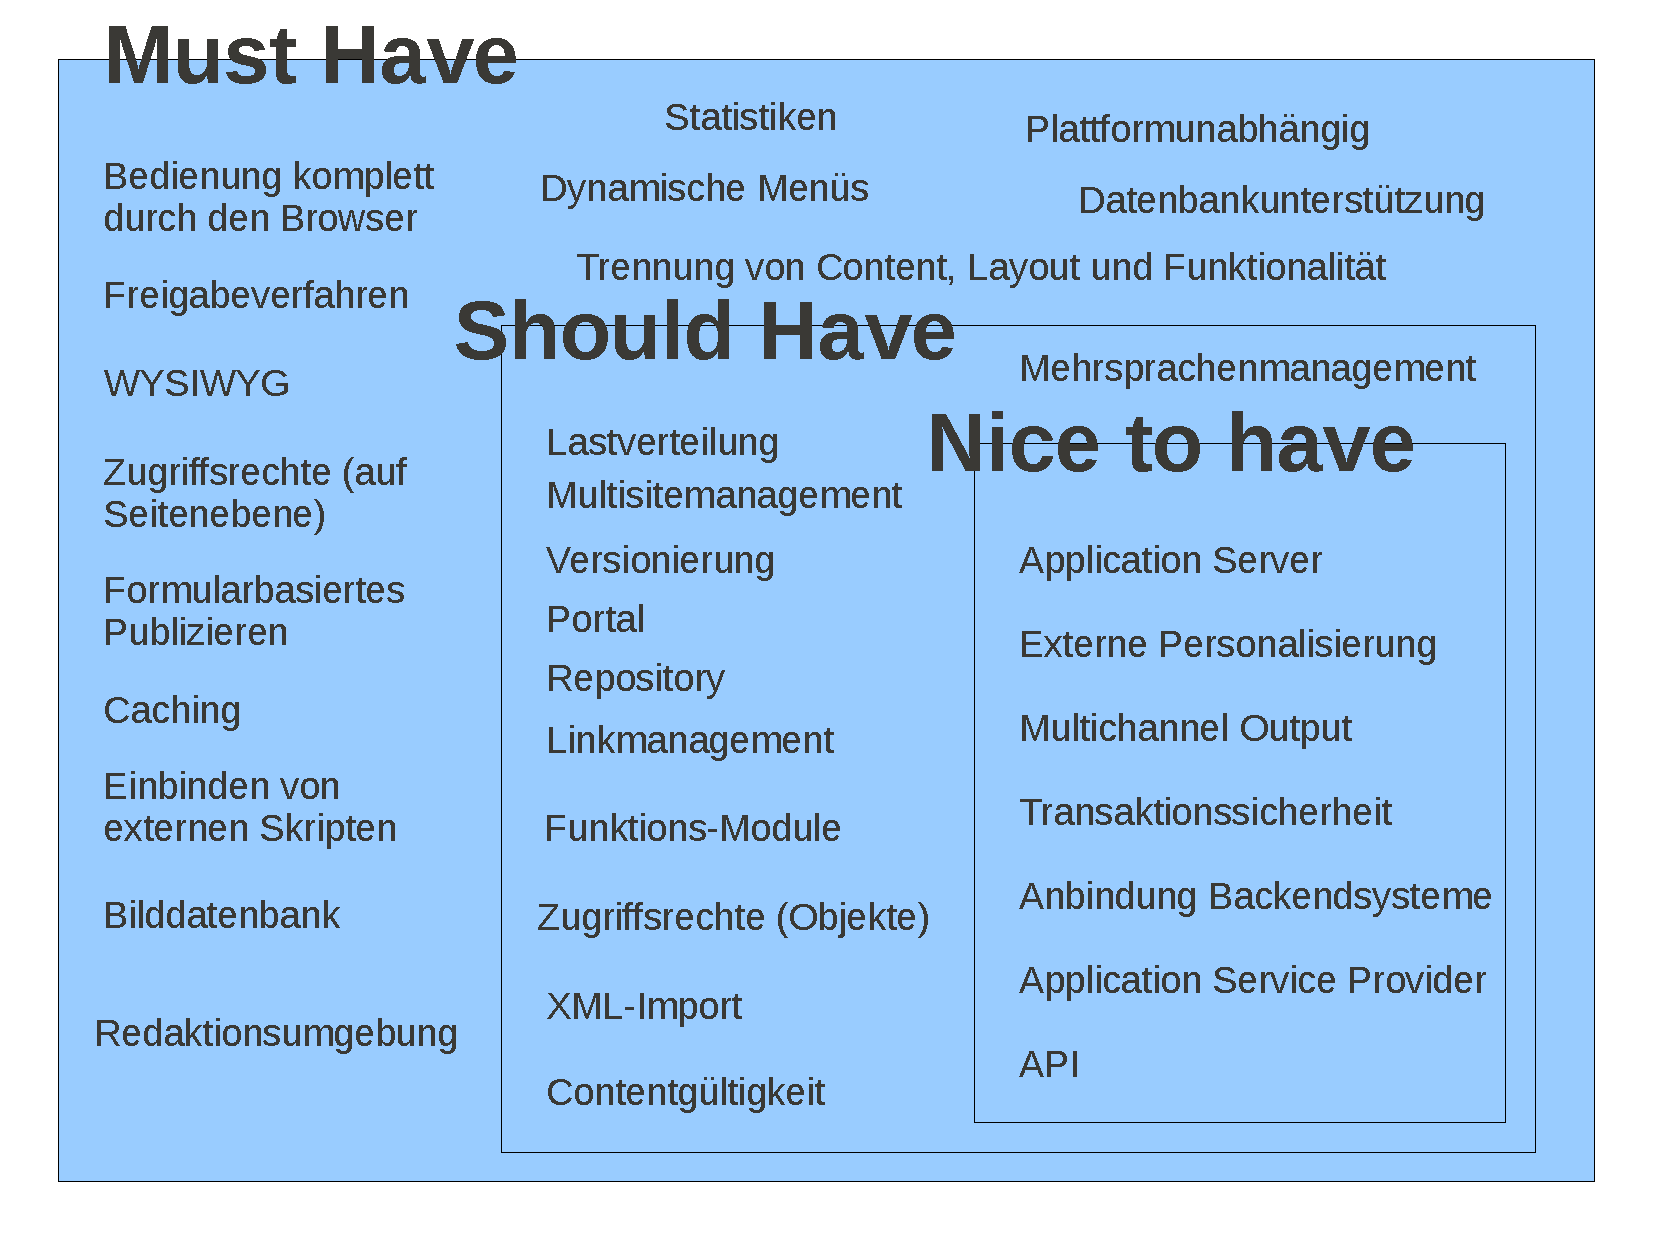
\includegraphics[scale=0.5]{images/analyse/featurematrix.pdf}
\caption[Feature-Matrix für Web Content Management Systeme]{Feature-Matrix für Web Content Management Systeme. Quelle: Eigene Darstellung nach \citep{jdkmatrix}.}
\label{featurematrix}
\end{center}
\end{figure}

Die beschriebenen Funktionalitäten sind jedoch teilweise so allgemein formuliert, das dieser Ansatz nur als grobe Orientierungshilfe dienen kann. Der Wirtschaftsinformatiker Andreas Ritter hat daher im Rahmen seiner Bachelorarbeit \emph{SWOT-Analyse zu Content-Management-Systemen} \cite{RitterSwot} Bereichskriterien erarbeitet, an Hand deren die Leistungsfähigkeit von Web Content Management Systemen untersucht werden kann \citep[][Seite 21-23]{RitterSwot}. Auf Grundlage dieser Bereichskriterien und der vorgestellten WCMS-Featurematrix wird in den Kapiteln \ref{sec:erstellung} bis \ref{sec:archi} ein Kriterienkatalog vorgestellt, der allgemeine Funktionalitätsanforderungen unterteilt nach den einzelnen Teilprozessen des Content Life Cycle (Erstellung, Kontrolle, Freigabe, Publikation, Archivierung) formuliert.

\subsection{Erstellung}
\label{sec:erstellung}
\begin{itemize}
\item
In einem WCMS sollen mehrere Redakteure Inhalte gleichzeitig erstellen, ändern, löschen und verwalten können.
\item
In einem WCMS sollen Inhalte – unabhängig von Zeit und Standort – durch mehrere Benutzer online verwaltet und erfasst werden können.
\item
In einem WCMS soll eine Offline-Erfassung von Inhalten unter Verwendung eines lokal auf dem Rechner installierten Programms möglich sein.
\item
Das WCMS verfügt über eine integrierte Mediendatenbank zur Erfassung und Verwaltung von Bildern, Multimedia, Texten, Audio, Videos, usw. Die Inhalte werden dabei in einer Datenbank gespeichert.
\item
Inhalte sollen in einem WCMS ohne spezielle Programmier- und HTML-Kenntnisse erfasst und verwaltet werden können.
\item
Die Nutzung des WCMS erfolgt über einen Internet-Browser. Dabei können alle gängigen Internet-Browser (Internet Explorer, Safari und Firefox) eingesetzt werden.
\item
Ein WCMS soll Inhalte mehrsprachig erfassen und verwalten können.
\item
Inhalte können in einem WCMS während der Erfassung über eine Preview-Funktion vorab im Design der Webseite betrachtet werden.
\item
Das WCMS ermöglicht eine Zuordnung von standardisierten und frei definierbaren Metadaten zu beliebigen Inhalten (z.B. Autor, Schlüsselwörter, benutzerdefinierte Felder).
\item
Das CMS soll über eine offene API (Programmierschnittstelle) für individuelle Erweiterungen verfügen.
\item
Das WCMS ermöglicht die Integration von Inhalten anderer Webseiten, Applikationen oder E-Commerce- Tools.
\item
In einem WCMS sollen Inhalte einfach importiert und exportiert werden können. Beim Austausch kommen Formate wie z.B. XML zum Einsatz.
\end{itemize}



%#### end Erstellung

\subsection{Kontrolle}


\begin{itemize}
\item
Das WCMS verfügt über ein granulares Rechte- und Rollenkonzept für Anwender, Inhalte, Module (Plugins) und Webseiten.
\item
Das WCMS ermöglicht die Versionierung von Inhalten. Zusätzlich können vorhergehende Zustände/Versionen mit Hilfe einer Wiederherstellungsfunktion rekonstruiert werden.
\item
Das WCMS bietet einen Schutz vor gegenseitigem Überschreiben erfasster Inhalte durch z.B. Check in/ Check out- Mechanismen.
\item
Das WCMS ist mandantenfähig, d.h. eine Mehrfachnutzung des Systems durch verschiedene Parteien mit kompletter Trennung der Daten und Benutzer ist möglich.
\item
Das WCMS bietet eine Linküberprüfung, die eine korrekte Darstellung von internen und externen Links auf der Internetseite sicherstellt.
\end{itemize}

%######## end kontrolle

\subsection{Freigabe}

\begin{itemize}
\item
Mit Hilfe des WCMS können \emph{nicht technische} User den Workflowprozesse kreieren, verwalten und ändern. Es sollen dafür keine Programmierkenntnisse notwendig sein.
\item
Das WCMS bildet einen mehrstufigen Workflowprozess für die Freischaltung von Inhalten ab.
\item
Das WCMS bietet die Möglichkeit, externe Mitarbeiter in Workflowprozesse einzubinden.
\item
Unternehmensspezifische Bearbeitungsprozesse von Inhalten sollen über frei definierbare Workflows verwaltet werden können.
\end{itemize}

%##### end freigabe


\subsection{Publikation}

\begin{itemize}
\item
Das WCMS trennt Inhalt und Design durch die Verwendung von Templates.
\item
Das WCMS erlaubt die Mehrfachverwendung von Inhalten an verschiedenen Stellen (auf unterschiedlichen Seiten).
\item
Das WCMS ermöglicht die Wahl zwischen dynamischer oder statischer Generierung der Seiten bzw. Inhalte (Caching).
\item
Das WCMS bietet Möglichkeiten, Inhalte für anderen Webseiten bereitzustellen (z.B. XML, Webservice).
\item
Navigationsstrukturen werden vom WCMS automatisch generiert, publiziert und verwaltet.
\item
Das WCMS bietet eine automatische Erstellung von Druckversionen und Weiterempfehlung einer Webseite.
\item
Inhalte sollen vom WCMS auf verschiedene Medien / Technologien (Cross Media Publishing, SMS / Mobile / WAP / usw.) ausgegeben werden können.
\item
Das WCMS ermöglicht ein barrierefreies Publizierten der erstellten Seiten.
\end{itemize}

%############## end publikation

\subsection{Terminierung und Archivierung}
\label{sec:archi}
\begin{itemize}
\item
Im WCMS können Inhalte und Seiten archiviert werden.
\item
Das WCMS erlaubt die freie Wahl des Publikationszeitraumes (zeitgesteuertes Auf- / Abschalten / Archivieren) von Inhalten.
\item
Das WCMS ermöglicht eine Durchsuchung der archivierten Inhalte und Seiten nach wählbaren Parametern (z.B. Monat oder Jahr).
\end{itemize}

%############## end terminierung


\chapter{Funktionale Analyse der bestehenden Web Content Management Systeme}


\section{Vorbetrachtungen}
Der 2006 eingeleitete Hype um das Ruby on Rails Framework hat dazu geführt, dass viele Entwickler mit der Konzeption und Umsetzung zahlreicher verschiedener Rails-Anwendungen begonnen haben. So entstanden auch im Bereich der Web Content Management Systeme zahlreiche Projekte. Ein Großteil der Vorhaben blieb jedoch in der Konzeptionsphase stecken oder die Entwicklung wurde nach wenigen Jahren eingestellt. Die Ursachen sind dabei vor allem dem Entwicklungsumfeld von Rails und dem Framework selbst geschuldet:


\begin{description}
\item[Schnellebigkeit]\mbox{~}\\*
Die Entwicklung des Ruby on Rails Frameworks unterliegt einem ständigen Wandel und erfordert eine ständige Anpassung des Programmierers an neue Technologien und Konzepte.
\item[Interessenwandlung der Entwickler]\mbox{~}\\*
Die elegante Programmierung mit Ruby und die vielfältigen Möglichkeiten des Ruby on Rails Frameworks erleichtern die Umsetzung verschiedenster Projektideen.
Es ist daher schneller möglich, dass sich Entwickler nach einiger Zeit mit anderen Projekten beschäftigen und bestehende Projekte vernachlässigen\footnote{Im Anhang der Arbeit findet sich eine Übersicht zu ermittelten Rails 2 und 3 Web Content Management Systemen. Diese sind zum Teil seit einigen Jahren nicht mehr weiterentwickelt wurden.}.
\end{description}

Die Realisierung eines stabilen Web Content Management Systems auf Basis von Ruby on Rails wird durch diese Faktoren erschwert und erfordert ein entsprechend tragfähiges Konzept sowie planendes Vorgehen der Projektiniziatoren.

Die hier aufgeführten Projekte Alchemy CMS, Browser CMS, Locomotive CMS und Refinery CMS repräsentieren daher die zum Zeitpunkt der Erstellung dieser Arbeit vielversprechendsten Rails-Implementierungen eines Web Content Management Systems. Trotz alldem ist anzumerken, dass sich diese Systeme, im Gegensatz zu anderen etablierten Web Content Management Systemen wie Typo3 und Drupal, noch am Anfang ihrer Entwicklungsgeschichte befinden.
\newline
\newline
Um die Zahl der zu untersuchenden WCMS einzuschränken, wurden folgende Mindestanforderungen für existierende Rails-Anwendungen festgelegt:
\begin{description}
\item[Open Source Software]\mbox{~}\\*
Die hier ermittelten WCM-Systeme sind vollständige Open Source Lösungen. Ihre Veröffentlichung unterliegt dabei den in der Open Source Bewegung üblichen Lizenzen der Freien Software bzw. der Open Source Initiative (OSI).
\item[Rails 3 Kompatibilität]\mbox{~}\\*
Die Veröffentlichung von Rails 3 brachte vielen Verbesserungen hinsichtlich der Modularität von Rails-Anwendungen. Kern-Komponenten des Frameworks (z.B. die Persistenz-Schicht Active Record) können nun mit geringem Aufwand gegen andere Implementierungen ausgetauscht werden. Die so erreichte Flexibilität soll auch bei der Integration eines Rails WCM-Systems zur Verfügung stehen.	Weiterhin sichert die Verwendung der aktuellsten Framework-Version die 	Unterstützung moderner Technologien und Entwicklungen innerhalb der implementierten WCMS ab.
\item[Aktive Entwicklung]\mbox{~}\\*
Die stetige, aktive Entwicklung an einem Open Source Projekt ist ein Merkmal für die Akzeptanz einer Software. Sie ist zusätzlich ein Beweis für das Engagement der beteiligten Programmierer. Eine in diesem Umfeld entstehende Software bietet daher entsprechend höheres Potenzial. Die  hier ausgewählten Systeme erfüllen diese Forderung.
\newpage
\item[Unterscheidung in Front- und Backend]\mbox{~}\\*
WCM-Systeme unterscheiden zwischen Frontend- und Backend-Funktionalität. Das Frontend wird durch die eigentliche Internetseite repräsentiert, die mit Hilfe des Systems erzeugt wird. Im Backend können Anwender Inhalte zentral einpflegen und verwalten.
Die ausgewählten Implementierungen verfügen über eine solche konzeptionelle Trennung.
\end{description}

\section{Bezugsquellen}

Trotz der steigenden Bekanntheit von Ruby on Rails existiert zum Zeitpunkt der Anfertigung dieser Arbeit keine Fachliteratur, die sich mit den Möglichkeiten des Web Content Managements in Rails auseinandersetzt. Vielmehr sind folgende Schwerpunktsetzungen bei den verschiedenen Autoren festzustellen:
\begin{description}
\item[Grundlagenbücher]\mbox{~}\\*
Sie dienen als Einführung in Rails und verdeutlichen an Hand einfacher Anwendungen die Arbeitsweise mit dem Ruby on Rails Framework.
\item[Fortgeschrittene Techniken mit Ruby on Rails]\mbox{~}\\*
Rails Kern-Entwickler stellen ihre Erfahrungen mit dem Framework dar und geben Lösungsansätze für größere Unternehmensstrukturen und Projekte. Häufig vertiefte Themen sind dabei Skalierung, Performance und Refactoring.
\end{description}
Zur Ermittlung existierender Ruby on Rails Open Source WCMS-Software mussten daher alternative Informationsquellen herangezogen werden, die im folgenden kurz beschrieben werden sollen:
\begin{description}
\item[Anfragen im offiziellen IRC Channel von Ruby on Rails]\mbox{~}\\*
Der Ruby on Rails IRC Channel ermöglicht einen konstruktiven Austausch von Rails-Entwicklern zu verschiedenen Bereichen des Rails-Frameworks. Mit der Hilfe mehrerer hundert Nutzer täglich können so Probleme und Anfragen sehr umfassend beantwortet werden. Der Ruby on Rails Channel ist erreichbar unter \#rubyonrails.
\item[RubyGems.org]\mbox{~}\\*
Bibliotheken können die Funktionalität von Ruby enorm erhöhen. Zur Verbreitung dieser im Internet existiert u.a. der Ruby Online Community Anbieter RubyGems.org, der über 30.000 Erweiterungspakete verschiedenster Entwickler im Internet zum Download anbietet.
Der Dienst verfügt über eine ausführliche Suchfunktion, mit der gezielt nach bestimmten Bibliotheken gesucht werden kann. Neben einer kurzen Projektbeschreibung und Informationen zum Entwickler wird jedem Projekt ein Datum der letzten Aktualisierung zugeordnet. Der Entwicklungsstand eines Pakets kann so besser eingeschätzt werden. RubyGems.org stellt daher einen wichtigen Startpunkt zur Ermittlung existierender Ruby on Rails WCMS dar.
\begin{figure}[!h]
\begin{center}
\label{fig.rubygems}
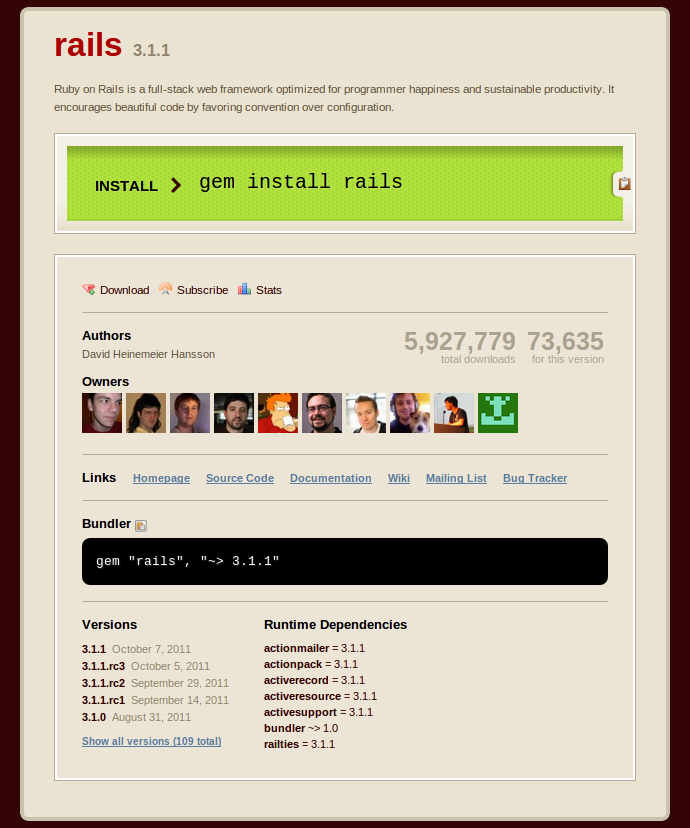
\includegraphics[scale=0.3]{images/analyse/rubygems/railsonrubygems.png}
\caption{Ruby Gems mit aufgelisteten Informationen zum aktuellen Rails 3.1}
\end{center}
\end{figure}
\newpage
\item[Github.com]\mbox{~}\\*
Github.com ist ein Online-Netzwerk und Webhosting-Dienst für Programmierer. Nutzer können dort ihre individuellen Programme, umgesetzt in beliebigen Programmiersprachen, kostenlos\footnote{Die Einrichtung eines kostnpflichtigen, privaten Github-Repositories ist ebenfalls möglich.}  veröffentlichen.
Schlüsseltechnologie des Netzwerkes ist das Versionsverwaltungssystem Git\footnote{PRojektseite: \href{http://git-scm.com/}{http://git-scm.com/}}, welches Änderungen am Quellcode des Projektes festhält. Zusätzlich erlaubt es anderen Programmierern, bestehende Projekte zu kopieren und eigenständig weiterzuentwickeln. Anschließend können diese wieder zu einem Gesamtprojekt verschmolzen werden.
Die Symbiose zwischen den Funktionalitäten von Git und den zahlreichen Interkationsmöglichkeiten der Platform erschaffen eine Entwicklungsumgebung, in der ein schneller und effektiver Austausch zwischen Programmierern und Projekten stattfinden kann.
Innerhalb der Ruby on Rails Community hat sich Github zu einer zentralen Anlaufstelle für Rails-Programmierer entwickelt und besitzt daher zur Ermittlung bestehender Web Content Management Systeme entscheidende Relevanz.
\begin{figure}[!h]
\begin{center}
\label{fig.github}
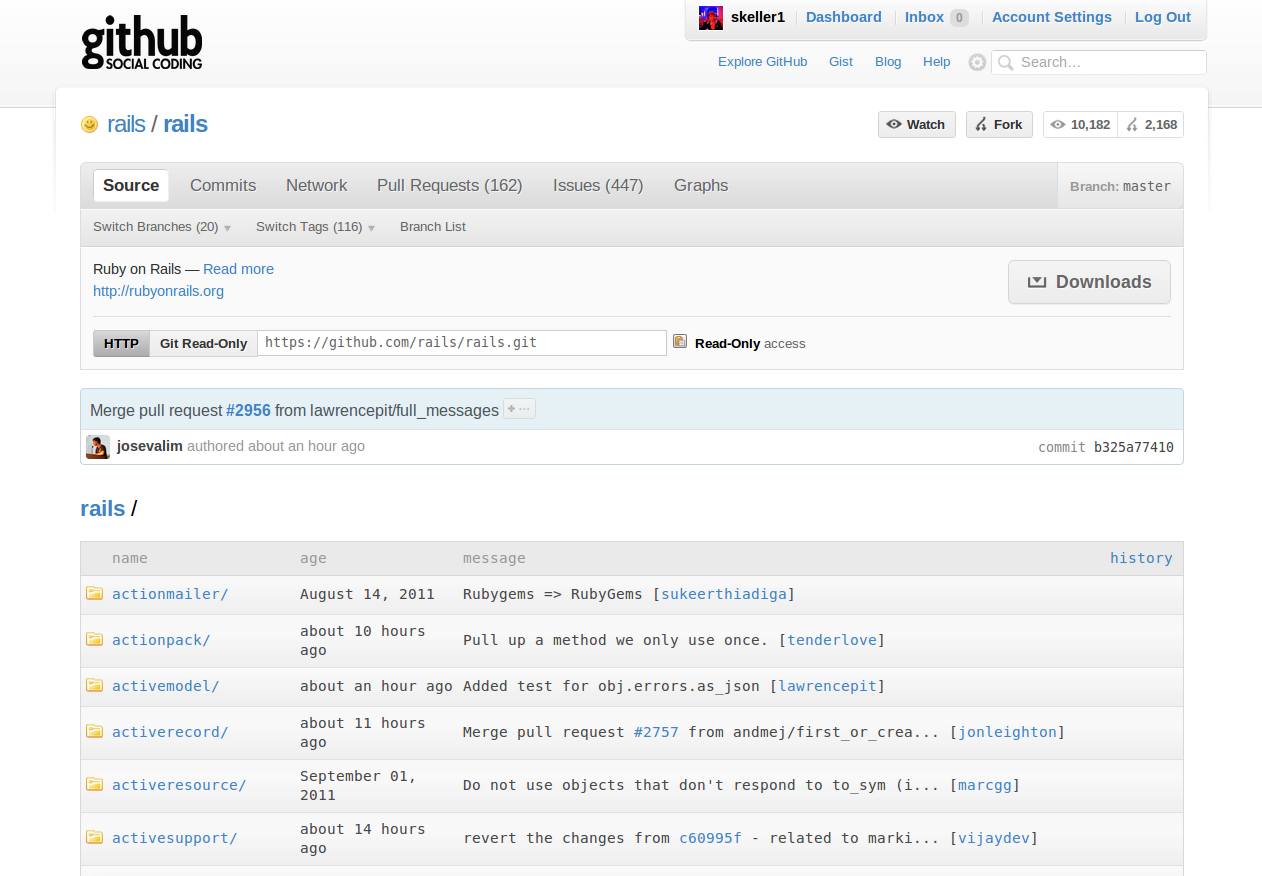
\includegraphics[scale=0.3]{images/analyse/github/github.png}
\caption{Beispiel für ein öffentliches Projekt auf Github.com: Das ausgewählte Projekt ist Rails 3}
\end{center}
\end{figure}
\end{description}

%ALCHEMY BEGIN
\pagebreak
\section{Vorstellung Alchemy CMS}
Unter der Leitung der Hamburger Firma \emph{macabi} wurde 2007 die proprietäre CMS Software \emph{WashAPP} veröffentlicht. Nach der Insolvenz der Entwickler wurde das System zu nächst weiterverkauft (dabei erfolgte die Umbennung in \emph{Webmate}), bevor es 2010 letztendlich als Open Source Software Alchemy CMS an die Öffentlichkeit übergeben wurde. Die Weiterentwicklung übernimmt seitdem die Hamburger Internetagentur \emph{magiclabs*}\footnote{Homepage: \href{http://magiclabs.de/home}{http://magiclabs.de/home}} um die Entwickler Thomas von Deyen, Robin Böning und Carsten Fregin. Die aktuelle Version 1.6.0 steht als Rails 2 und 3 Umsetzung\footnote{Der Rails 3-Entwicklungszweig von Alchemy befindet sich noch im Beta-Stadium.} zur Verfügung.
\begin{table}[!h]
\caption{Steckbrief Alchemy CMS}
\begin{tabular}[!ht]{|l|l|l|}
\hline
\textbf{Aktuelle Version} & \multicolumn{2}{p{10cm}|}{1.6.0} \\
\hline
\textbf{Lizenz} & \multicolumn{2}{p{10cm}|}{GPLv3} \\
\hline
\textbf{Projektseite} & \multicolumn{2}{p{10cm}|}{\href{http://alchemy-cms.com}{http://alchemy-cms.com}} \\
 & \multicolumn{2}{p{10cm}|}{\href{https://github.com/magiclabs/alchemy}{https://github.com/magiclabs/alchemy}} \\
\hline
\textbf{Quellcode} & \multicolumn{2}{p{10cm}|}{\href{https://github.com/magiclabs/alchemy}{https://github.com/magiclabs/alchemy}} \\
\hline
\textbf{IRC-Channel} & \multicolumn{2}{p{10cm}|}{nicht vorhanden} \\
\hline
\textbf{API Dokumentation} & \multicolumn{2}{p{10cm}|}{nicht verfügbar} \\
\hline
\textbf{Forum} & \multicolumn{2}{p{10cm}|}{\href{http://groups.google.com/group/alchemy-cms}{http://groups.google.com/group/alchemy-cms}} \\
\hline
\textbf{Demoversion} & Frontend & \href{http://demo.alchemy-cms.com}{http://demo.alchemy-cms.com} \\
\cline{2-3}
& Backend & \href{http://demo.alchemy-cms.com/admin}{http://demo.alchemy-cms.com/admin} \\
\cline{2-3}
& Login & demo \\
\cline{2-3}
& Passwort & demo \\
\hline
\textbf{Verwendete Technologien} & \multicolumn{2}{p{10cm}|}{Ruby on Rails 3.0.x, HTML, jQuery und jQueryUI, TinyMCE - Javascript WYSIWYG Editor, SWFUpload} \\
\hline
\textbf{Projektbeschreibung} & \multicolumn{2}{p{10cm}|}{Alchemy ist ein unglaubliches Content Managment System, welches sich gut in Rails integrieren lässt. – Absolut flexibel und kraftvoll.} \\
\hline
\textbf{Philosophie} & \multicolumn{2}{p{10cm}|}{Der Benutzer des Systems muss nur Inhalte erstellen und ändern können} \\
& \multicolumn{2}{p{10cm}|}{Formatierung von Überschriften, Bildpositionierung und -berechnung sind Aufgaben des Entwicklers, nicht die des Redakteurs}\\
\hline
\textbf{Zielgruppe} & \multicolumn{2}{p{10cm}|}{Privatnutzer, Kleinstunternehmen} \\
\hline
\end{tabular}
\end{table}

\subsection{Funktionsprinzipien}
Das Backend von Alchemy CMS verfügt u.a. über die Bereiche Seiten, Sprachen, Benutzer und Bibliothek:
\begin{figure}[!h]
\begin{center}
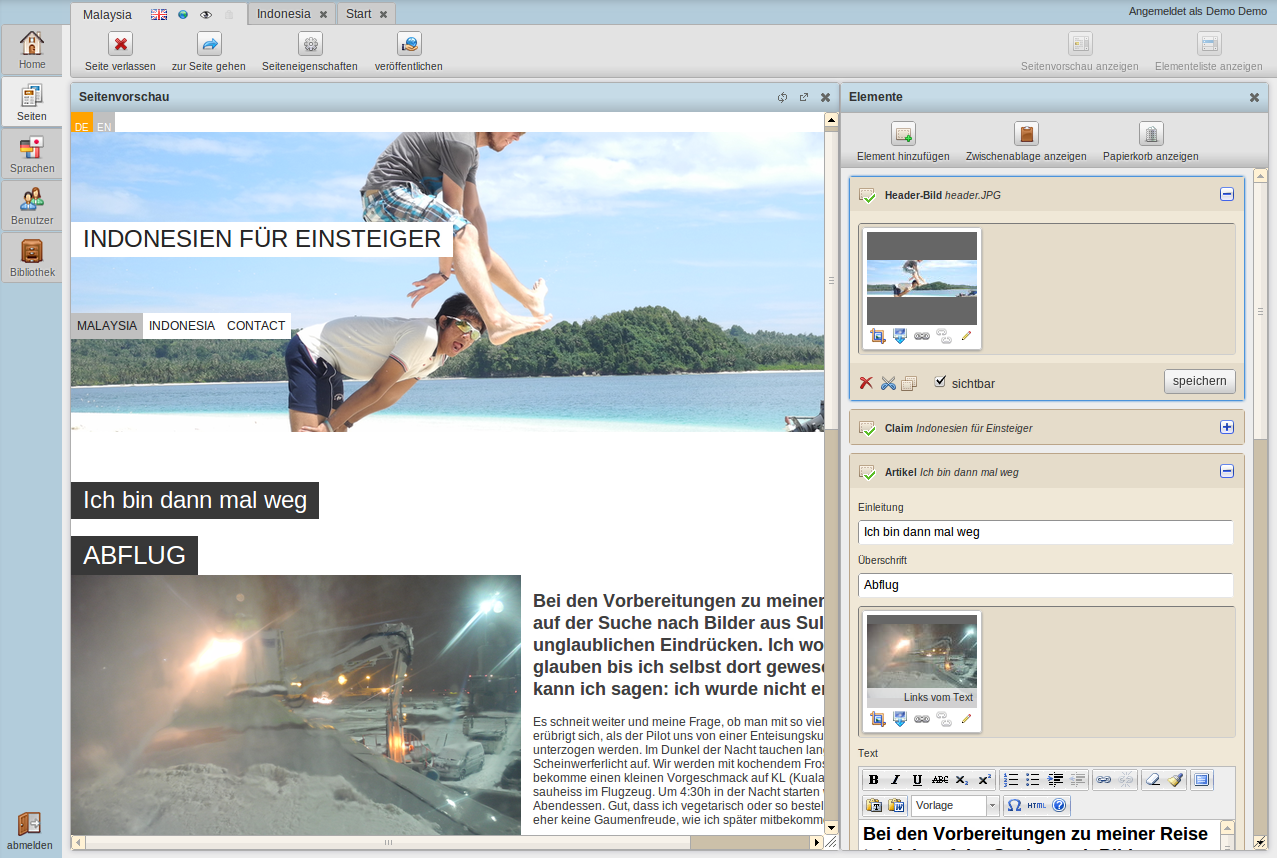
\includegraphics[scale=0.3]{images/analyse/alchemy/inhalte.png}
\caption{Backend-Ansicht von Alchemy CMS mit geöffnerter Seitenvorschau und Elementebearbeitung}
\label{alchemybackend}
\end{center}
\end{figure}

\begin{description}
\item[Home]\mbox{~}\\*
Nach einer erfolgreichen Anmeldung im Backend bildet das Home-Modul eine Art Startseite, in der der Nutzer über die letzten Aktivitäten des Systems informiert wird (z.B. Auflistung der zuletzt editierten Inhalte).
\item[Seiten]\mbox{~}\\*
Im Seiten-Modul des Backends findet die Verwaltung aller im System angelegter Seiten und deren Inhalte statt. Eine abgebildete Baumstruktur ermöglicht dabei einen Überblick über die verwalteten Seiten des Systems. Im Bearbeitungsmodus bietet Alchemy CMS darüber hinaus eine Aufteilung der Ansicht in einen Vorschaubereich, der die aktuell ausgewählte Seite mit ihren tatsächlichen Inhalten anzeigt, und einem Elemente-Bereich, der die auf der Seite verfügbaren Inhalselemente angibt und editierbar macht (Abb. \ref{alchemybackend}).
\item[Sprachen]\mbox{~}\\*
Diese Modul ermöglicht die komfortable Verwaltung der in Alchemy CMS verfügbaren Frontend-Sprachen. Eine Alchemy Standard-Installation enthält bereits die Sprachen Deutsch und Englisch.
\item[Benutzer]\mbox{~}\\*
Das Benutzer-Modul ist die zentrale Anlaufstelle zur Verwaltung der am System registrierten Administratoren, Autoren und Redakteure sowie ihrer jeweiligen Befugnisse innerhalb des CMS.
\item[Bibliothek]\mbox{~}\\*
Bilder und andere Dateien werden in Alchemy CMS über das Bibliotheken-Modul verwaltet. Es ermöglicht die Auflistung aller im System zur Verfügung stehenden Ressourcen. Zusätzlich stehen Funktionen zum Hochladen, Editieren und Löschen von Ressourcen zur Verfügung.
\end{description}
\subsection{Erweiterungen}
Alchemy kann durch die Erstellung von Plugins in seiner Funktionalität erweitert werden. An Hand einer definierten API wird ein Grundgerüst angeboten, mit deren Hilfe Erweiterungen bequem in alle Teile des Systems integriert werden können. Ein Plugin kann so entweder als neues Backend-Modul umgesetzt werden (es erscheint in Form eines neuen Menüeintrages im linken Bereich des Backends) oder neue Inhaltselemente zur Verfügung stellen, die dann innerhalb der Seitenbearbeitung als auswählbarer Inhaltstyp zur Verfügung stehen (Abb. \ref{img.alchemycontenttypes}).
\newline
\newline
Folgende offiziellen Erweiterungen sind ebenfalls verfügbar:
\begin{itemize}
\item
alchemy-mailings\footnote{Komponenten-Download: \href{https://github.com/magiclabs/alchemy-mailings}{https://github.com/magiclabs/alchemy-mailings}}: Ermöglicht die Erstellung und Verwaltung von Newsletters im Backend des Systems.
\item
alchemy-standard-set\footnote{Komponenten-Download: \href{ https://github.com/magiclabs/alchemy-standard-set}{ https://github.com/magiclabs/alchemy-standard-set}}: Enthält CSS-Formatierungen für die in Alchemy verfügbaren Standard-Inhaltselemente.
\end{itemize}

\begin{figure}[!h]
\begin{center}
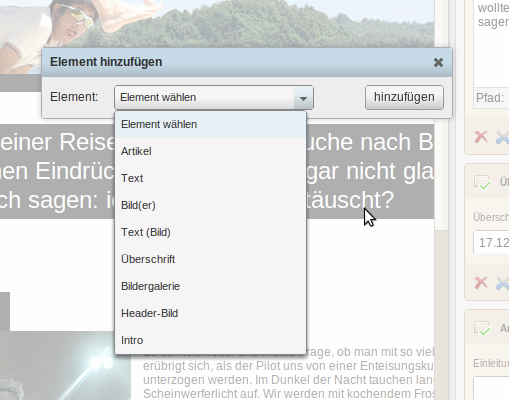
\includegraphics[scale=0.6]{images/analyse/alchemy/dialoginhaltselement.png}
\caption{Standardset von Inhaltselementen in Alchemy CMS}
\label{img.alchemycontenttypes}
\end{center}
\end{figure}



\subsection{Verwendete Technologien}
Schwerpunkttechnologien der Nutzeroberfläche von Alchemy CMS sind die an Hand von Rails erzeugten HTML-Views und darin eingebundene JavaScript-Dateien, die mit Hilfe des JavaScript Frameworks jQuery erstellt wurden.
Das Seiten-Modul greift zusätzlich auf die jQuery UI Bibliothek zurück, die vorgefertigte Elemente zur Erstellung von Dialogboxen und dem Tabulator-Menü liefert.
Der bei einigen Inhaltselementen verfügbare WYSIWJG-Javascript Editor TinyMCE ermöglicht die Formatierung einzelner Inhalte und das Einfügen von vorgefertigtem HTML.
Ein Hochladen von Ressourcen erfolgt in Alchemy über ein herkömmliches HTML Upload-Feld oder den integrierten Adobe Flash Uploader, der somit auch das Einstellen mehrerer Medien in einem Schritt ermöglicht.
%ALCHEMY END


%Browser BEGIN


\newpage
\section{Vorstellung Browser CMS}
Browser CMS ist ein Open Source Web Content Management System der US-amerikanischen Agentur BrowserMedia mit Sitz in Bethesda, Maryland. Im Gegensatz zum aktuellen Versionszweig 3.x des Systems wurden die Vorgängerversionen (Versionen 1.x und 2.x) mit Hilfe der Java Programmiersprache umgesetzt.
Auf Grund geänderter Marktsituation entschied sich BrowserMedia jedoch 2009 dazu, alle weiteren Versionen des CMS auf Grundlage des Rails Frameworks\footnote{Ausführliche Informationen zum Übergang von Java auf Rails können unter folgender Quelle nachvollzogen werden: href{http://tinyurl.com/6eayba7
}{http://tinyurl.com/6eayba7}} zu entwickeln. Zusätzlich erfolgte der Umstieg auf die GPLv3-Lizenz, die eine freie Verwendung der Software ermöglicht.
Eine online verfügbare Testversion des Systems wird von BrowserMedia nicht angeboten. Um dennoch die Funktionalität des Systems zu demonstrieren, wurde eine Installation  von Browser CMS 3.3.1 eingerichtet\footnote{Die Upload-Funktion des CMS wurde auf Grund zu geringer Server-Ressourcen deaktiviert.}.
\begin{table}[!h]
\caption{Steckbrief Browser CMS}
\begin{tabular}[!ht]{|l|l|l|}
\hline
\textbf{Aktuelle Version} & \multicolumn{2}{p{10cm}|}{3.3.1} \\
\hline
\textbf{Lizenz} & \multicolumn{2}{p{10cm}|}{GPLv3} \\
\hline
\textbf{Projektseite} & \multicolumn{2}{p{10cm}|}{\href{http://browsercms.org}{http://browsercms.org}} \\
\hline
\textbf{Quellcode} & \multicolumn{2}{p{10cm}|}{\href{https://github.com/browsermedia/browsercms
}{https://github.com/browsermedia/browsercms}} \\
\hline
\textbf{IRC-Channel} & \multicolumn{2}{p{10cm}|}{nicht vorhanden} \\
\hline
\textbf{API Dokumentation} & \multicolumn{2}{p{10cm}|}{\href{http://rubydoc.info/gems/browsercms/
}{http://rubydoc.info/gems/browsercms/}} \\
\hline
\textbf{Forum} & \multicolumn{2}{p{10cm}|}{\href{http://groups.google.com/group/browsercms}{http://groups.google.com/group/browsercms}} \\
\hline
\textbf{Demoversion} & Frontend & \href{http://diplomabcms.heroku.com/}{http://diplomabcms.heroku.com/} \\
\cline{2-3}
& Backend & \href{http://diplomabcms.heroku.com/cms}{http://diplomabcms.heroku.com/admin} \\
\cline{2-3}
& Login & demo \\
\cline{2-3}
& Passwort & demo \\
\hline
\textbf{Verwendete Technologien} & \multicolumn{2}{p{10cm}|}{Ruby on Rails 3.0.x, HTML, jQuery und jQueryUI, diverse jQuery Plugins ,WYSIWYG-HTML-Editor CKEditor} \\
\hline
\textbf{Projektbeschreibung} & \multicolumn{2}{p{10cm}|}{Menschliches Content Management mit Ruby on Rails 3 Unterstützung} \\
%\hline
%\textbf{Philosophie} & \multicolumn{2}{p{10cm}|}{Redakteuren soll es ermöglicht werden, ohne HTML- und Rails-Kenntnisse eine Internetseite zu verwalten} \\
\hline
\textbf{Zielgruppe} & \multicolumn{2}{p{10cm}|}{Privatnutzer, Kleine und mittelständige Unternehmen mit einer hohen Anzahl von Redakteuren} \\
\hline
\end{tabular}
\end{table}
\subsection{Funktionsprinzipien}

Innerhalb des Backend (Abb. \ref{browserbackend}) von Browser CMS kann der angemeldete Nutzer auf alle wichtigen Funktionsbereiche des Systems zugreifen:


\begin{figure}[!h]
\begin{center}
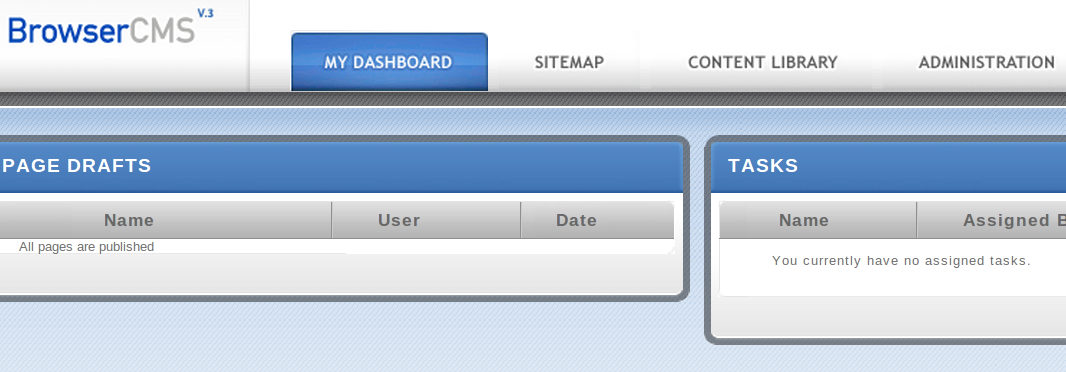
\includegraphics[scale=0.3]{images/analyse/browser/backend.png}
\caption{Backend-Ansicht von Browser CMS}
\label{browserbackend}
\end{center}
\end{figure}


\begin{description}
\item[Dashboard]\mbox{~}\\*
Das Dashboard gibt eine Übersicht über die zuletzt vom Nutzer bearbeiteten Seiten sowie eine Auflistung der vom Anwender noch zu erledigenden Aufgaben.
\item[Sitemap]\mbox{~}\\*
Das Sitemap-Menü ermöglicht die Darstellung aller im System existierenden Seiten in einer Baumstruktur sowie die Bearbeitung aller Informationen zu einer einzelnen Seite. U.a. kann der Titel, das verwendete Template und verschiedene Meta-Informationen verändert werden.
\item[Content Library]\mbox{~}\\*
In der Content Library von Browser CMS können alle existierenden Inhaltselemente sortiert nach Inhaltstyp (z.B. Text, File, Image) aufgelistet und bearbeitet werden.
\item[Administration]\mbox{~}\\*
Im Administrator-Bereich des Systems werden alle Gruppen und Nutzer des Backend und der Internetseite verwaltet. Zusätzlich können die für die einzelnen Seiten und Inhaltselemente definierten Templates aufgelistet und bearbeitet werden.
\end{description}

\begin{figure}[!h]
\begin{center}
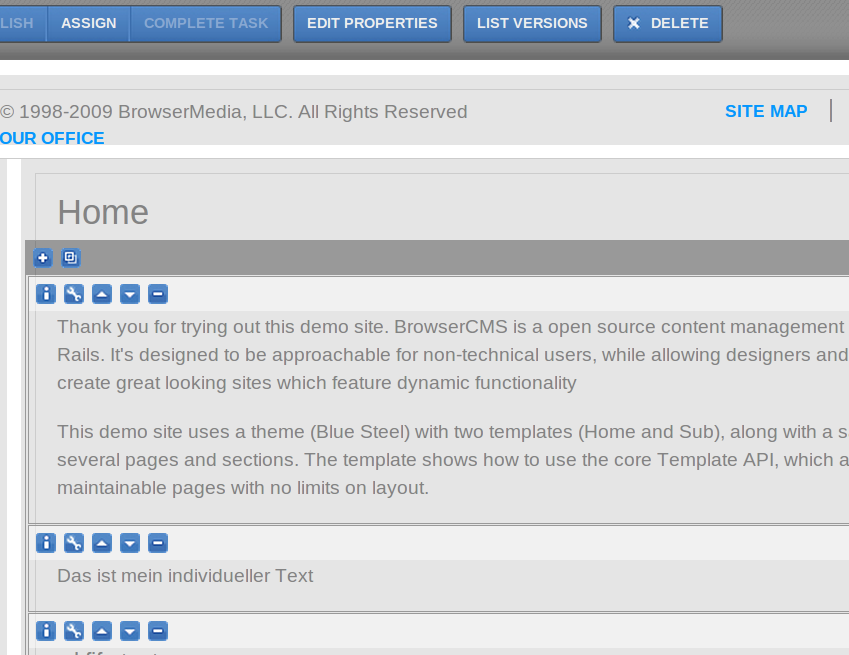
\includegraphics[scale=0.3]{images/analyse/browser/frontendangemeldet.png}
\caption{Ausgewählte Seite im Bearbeitungsmodus und aktiviertem Visual Editor}
\label{browserpageedit}
\end{center}
\end{figure}
Die Erstellung und Darstellung von Inhalten in Browser CMS wird durch folgende 2 Prinzipien realisiert:
\begin{description}
\item[Content Blocks]\mbox{~}\\*
Content Blocks sind Sammlungen von Daten mit einer definierten Anzahl an Feldern eines bestimmten Typs (z.B. Textfeld, Datumsfeld). Innerhalb der Content Library können diese verwaltet und angelegt werden.
\item[Portlet\footnote{Der Begriff des Portlets stammt aus der Java-Welt und bezeichnet ursprünglich beliebig kombinierbare Komponenten, die an verschiedenen Positionen auf einer Internetseite bzw. einer Portal-Seite dargestellt werden können.}]\mbox{~}\\*
Portlets sind spezielle Content Blocks, die festlegen, wie bereits existierende Content Blocks (z.B. Text, News) dargestellt werden sollen. Dazu verfügt jedes Portlet über ein im Backend editierbares Template, dass die zuvor ausgewählten Datensätze in dem gewünschten Layout präsentiert (Abb. \ref{browsertagportlet}).

\begin{figure}[!h]
\begin{center}
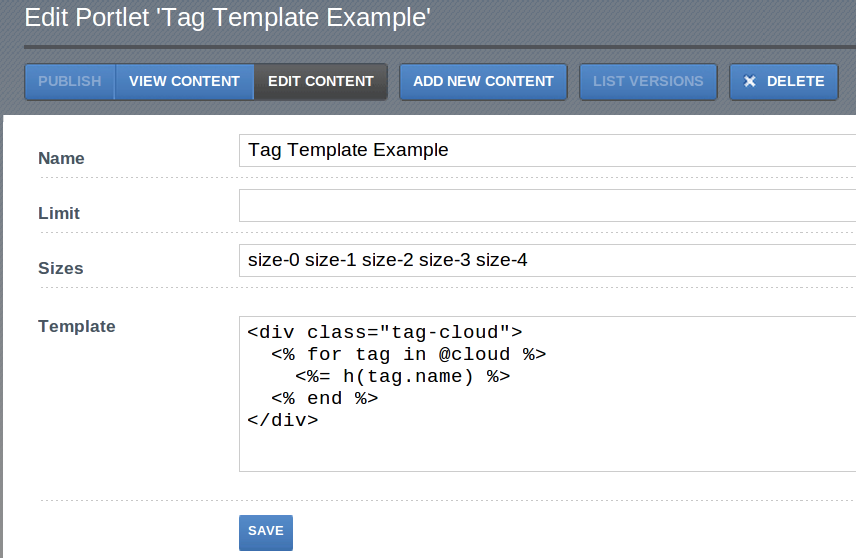
\includegraphics[scale=0.3]{images/analyse/browser/tagportlet.png}
\caption{Tag-Portlet mit Template im Backend von Browser CMS}
\label{browsertagportlet}
\end{center}
\end{figure}


\end{description}

\subsection{Erweiterungen}
Die Funktionalität von Browser CMS kann durch das Hinzufügen von sogenannten Modulen erweitert werden. Diese beinhalten dabei neue Content-Blocks oder vordefinierte Portlets, die in der Content Library des Backends verwaltet werden können. Im Internet stehen zusätzlich folgende vorgefertigten Erweiterungen bzw. Module zur Verfügung\footnote{Eine ausführliche Liste mit allen Erweiterungen findet sich unter folgender Adresse: \href{http://modules.browsercms.org/modules}{http://modules.browsercms.org/modules}}:


\begin{itemize}
\item browsercms-news\footnote{Komponenten-Download: \href{https://github.com/browsermedia/bcms\_news}{https://github.com/browsermedia/bcms\_news}}: Darstellung von kurzen Nachrichten im Frontend der Seite.
\item browsercms-blog\footnote{Komponenten-Download: \href{https://github.com/browsermedia/bcms\_blog}{https://github.com/browsermedia/bcms\_blog}}: Erstellung und Verwaltung von Blog-Einträgen inklusive Kommentar- und Tagging-Funktionalität.
\item browsercms-events\footnote{Komponenten-Download: \href{https://github.com/browsermedia/bcms\_event}{https://github.com/browsermedia/bcms\_event}}: Erstellung und Verwaltung von Event-Einträgen. Diese können wahlweise alle zusammen in einer Listenansicht oder in Einzeldarstellung individuell präsentiert werden.
\item browsercms-rankings\footnote{Komponenten-Download: \href{https://github.com/browsermedia/bcms\_rankings}{https://github.com/browsermedia/bcms\_rankings}}: Erlaubt dem Internetseitenbenutzer eine Bewertung der besuchten Seite abzugeben.
\end{itemize}

\subsection{Verwendete Technologien}

Das komplette Backend von Browsercms wird mit Hilfe von in Rails gerenderten HTML-Views erzeugt. JavaScript kommt lediglich bei der Darstellung verschiedener Feldtypen (z.B. Datumsdialog und Auswahlbox) innerhalb der Contentblöcke und beim Anlegen von Textinhalt durch die Verwendung des JavaScript-WYSIWYG-Editors FCKEditor (Abb. \ref{browsereditor}) zur Anwendung. Dieser ermöglicht die komfortable Formatierung eingestellter Texte sowie die Einbindung von vorformatierten HTML-Inhalten.

\begin{figure}[!h]
\begin{center}
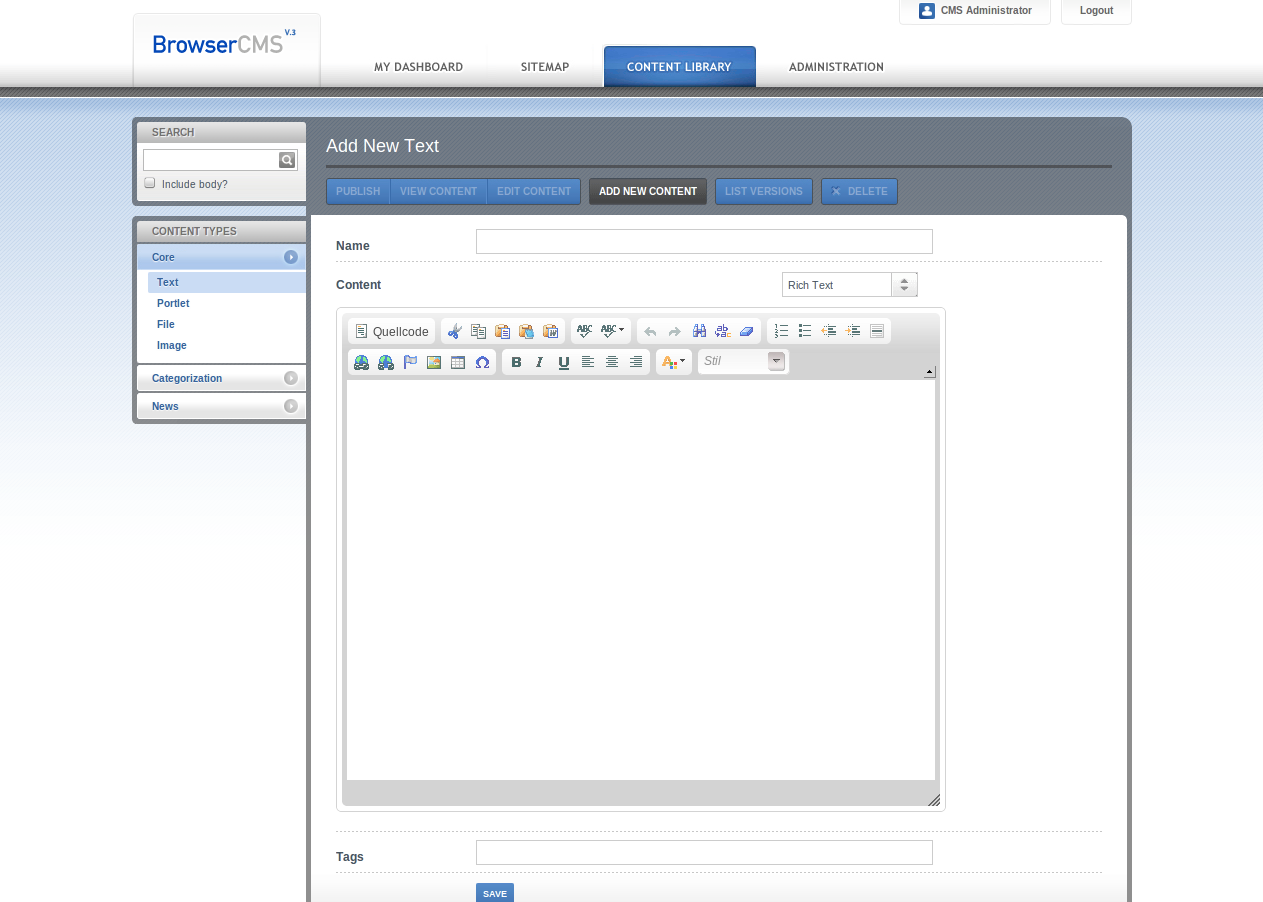
\includegraphics[scale=0.3]{images/analyse/browser/editor.png}
\caption{Erstellung eines neuen Content Blocks Text mit Hilfe des FCKEditor}
\label{browsereditor}
\end{center}
\end{figure}

Die Erstellung der Contentblöcke (Content Blocks) und Portlets wird durch einen in Rails umgesetzten Generatorskript ermöglicht und vereinfacht somit die Erstellung für den Entwickler. Er erzeugt ein komplettes


\lstinputlisting[caption=Aufruf des Generator-Skripts zur Erstellung eines neuen Inhaltselements Produkt]{code/content_block.rb}
%Browser END
\newpage
%Locomotive BEGIN
\section{Vorstellung Locomotive CMS}
Lokomotive CMS ist ein Open Source Content Management System der Ruby on Rails Entwickler Didier Lafforgue und Jacques Crocker sowie dem Designer Sacha Greif. Es wird unter der MIT Lizenz der Open Source Initiative vertrieben und steht in den Rails-Versionen 2 und 3 als Downloadpaket zur Verfügung. Neben den Möglichkeiten der eigenständigen Installation bieten die Initiatoren des Systems auch den kostenpflichtigen Dienst Bushi.do an, der eine automatische Installation von Lokomotive CMS vornimmt und es ermöglicht, nach wenigen Minuten sofort mit der Erstellung der Seite im Browser zu beginnen\footnote{Auf der Projektseite von Lokomotive CMS wird die automatische Installation mit Hilfe von Bushi.do beschrieben: \href{http://www.locomotivecms.com/}{http://www.locomotivecms.com/}}.
\begin{table}[!h]
\caption{Steckbrief Locomotive CMS}
\begin{tabular}[!ht]{|l|l|l|}
\hline
\textbf{Aktuelle Version} & \multicolumn{2}{p{10cm}|}{keine Angabe von Entwicklungsversionen} \\
\hline
\textbf{Lizenz} & \multicolumn{2}{p{10cm}|}{MIT License} \\
\hline
\textbf{Projektseite} & \multicolumn{2}{p{10cm}|}{\href{http://www.locomotivecms.com/}{http://www.locomotivecms.com/}} \\
\hline
\textbf{Quellcode} & \multicolumn{2}{p{10cm}|}{\href{https://github.com/locomotivecms/engine}{https://github.com/locomotivecms/engine}} \\
\hline
\textbf{IRC-Channel} & \multicolumn{2}{p{10cm}|}{\#locomotivecms} \\
\hline
\textbf{API Dokumentation} & \multicolumn{2}{p{10cm}|}{\href{http://rubydoc.info/github/resolve/refinerycms}{http://rubydoc.info/github/resolve/refinerycms}} \\
\hline
\textbf{Forum} & \multicolumn{2}{p{10cm}|}{\href{http://groups.google.com/group/refinery-cms/}{http://groups.google.com/group/refinery-cms/}} \\
\hline
\textbf{Demoversion} & Frontend & \href{http://diplomalocomotive.heroku.com/}{http://diplomalocomotive.heroku.com/} \\
\cline{2-3}
& Backend & \href{http://diplomalocomotive.heroku.com/admin}{http://diplomalocomotive.heroku.com/admin} \\
\cline{2-3}
& Login & demo@demo.de \\
\cline{2-3}
& Passwort & demo123 \\
\hline
\textbf{Verwendete Technologien} & \multicolumn{2}{p{10cm}|}{Ruby on Rails 3.0.x, HTML, jQuery und jQueryUI, diverse jQuery Plugins ,WYSIWYG-HTML-Editor Aloha und TinyMCE, MongoDB, Template Sprache Liquid} \\
\hline
\textbf{Projektbeschreibung} & \multicolumn{2}{p{10cm}|}{Locomotive ist ein Open Source CMS für Rails. Es ist sehr flexibel und unterstützt Heroku und Amazon S3.} \\
\hline
\textbf{Philosophie} & \multicolumn{2}{p{10cm}|}{Verwaltung kleiner Internetseiten} \\
& \multicolumn{2}{p{10cm}|}{Komplexe Inhaltselemente dank MongoDB selbst erstellen}\\
\hline
\textbf{Zielgruppe} & \multicolumn{2}{p{10cm}|}{Privatnutzer, Kleinstunternehmen} \\
\hline
\end{tabular}
\end{table}
\subsection{Funktionsprinzipien}
Locomotive CMS unterscheidet im Backend der Anwendung in folgende 2 Funktionsbereiche:
\begin{description}
\item[Inhalte]\mbox{~}\\*
Im Inhalte-Bereich des Backends werden alle im System angelegten Seiten und Inhaltselemente verwaltet und bearbeitet (Abb. \ref{locomotivebackend}). Die Darstellung jeder einzelnen Seite und der Inhaltselemente kann darüber hinaus durch Angabe eines Templates online verändert werden (mehr dazu in Abschnitt \ref{sec:TechnologienLocomotive}), was eine Umsetzung komplexer Seitenlayouts sicherstellt.
\begin{figure}[!h]
\begin{center}
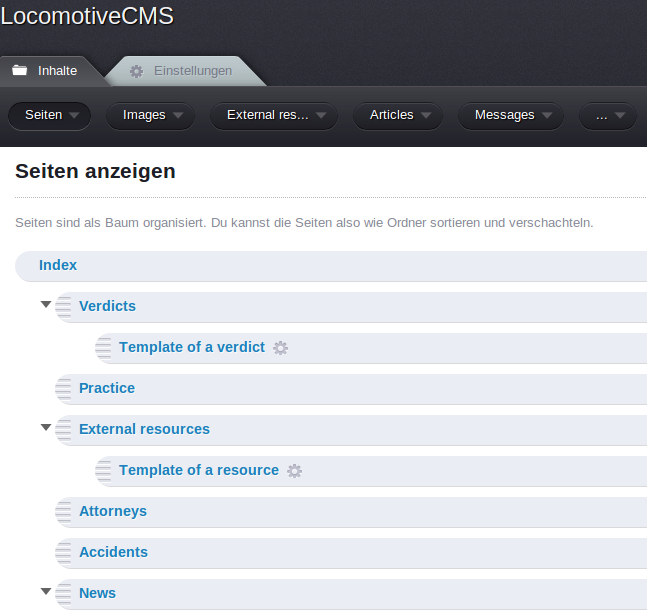
\includegraphics[scale=0.3]{images/analyse/locomotive/backendlocomotive.png}
\caption{Backend von Locomotive CMS mit geöffnetem Seitenbaum.}
\label{locomotivebackend}
\end{center}
\end{figure}
\item[Einstellungen]\mbox{~}\\*
Im Einstellungs-Modul befinden sich die zentralen Funktionen zur Bearbeitung der vorhandenen Backend-Nutzer sowie globaler Locomotive CMS-Einstellungen (registrierte Domains, Import-/Export von Seiten, Bearbeitung von allgemeinen Metainformationen des Systems). Zusätzlich können in einem Template-Bereich einzelne, zentrale Dateien verwaltet werden, die innerhalb des Seitenlayouts der Seite als Gestaltungselemente dienen sollen\footnote{Die für layoutspezifische Verwendung hochgeladenen Dateien werden in Locomotive CMS als Snippets bezeichnet}.
\end{description}
\subsection{Erweiterungen}
\label{sec:ErweiterungenLocomotive}
Erweiterungen werden in Locomotive CMS als Bausteine bezeichnet und repräsentieren individuell zusammengestellte Inhaltselemente. Sie können im Backend von Locomotive CMS über einen komfortablen Bearbeitungsdialog erstellt werden (Abb. \ref{locomotivecontent}). Im Gegensatz zu den hier bereits vorgestellten Systemen werden so keine Programmierkenntnisse der Anwender benötigt. Ebenfalls entfällt der Aufwand zur Installation einer Erweiterung.
\begin{figure}[!h]
\begin{center}
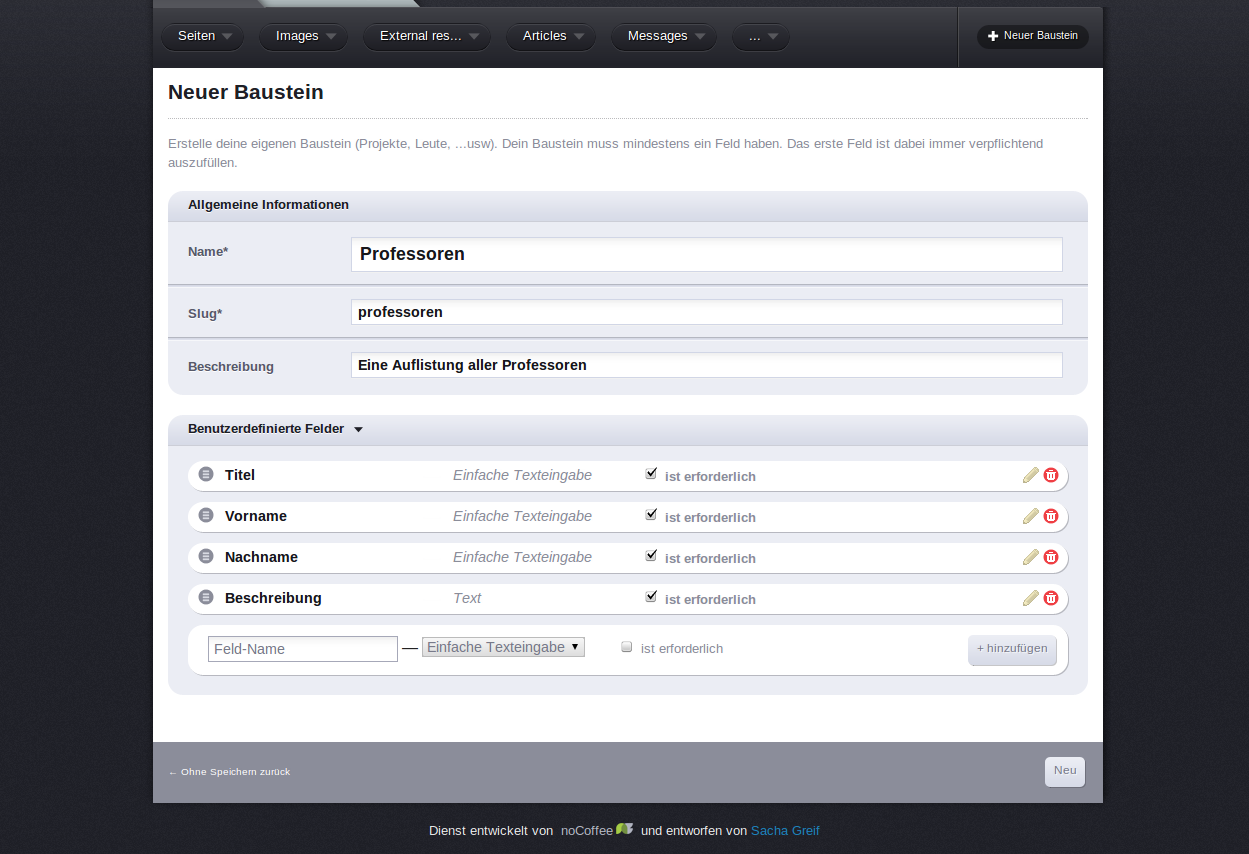
\includegraphics[scale=0.3]{images/analyse/locomotive/customcontent.png}
\caption{Ein im Backend von Locomotive CMS zusammengestelltes Inhaltselement}
\label{locomotivecontent}
\end{center}
\end{figure}
\newpage
Die Inhaltselemente können aus folgenden grundlegenden Feldtypen zusammengebaut werden:
\begin{itemize}
\item
Einfaches Textfeld
\item
Text
\item
Auswahlbox
\item
Checkbox
\item
Datum
\item
Datei
\item
has one (ermöglicht die Zuordnung genau eines anderen Inhaltselements des angegebenen Bausteintyps)
\item
has many (ermöglicht die Auswahl mehrerer anderer Inhaltselemente des angegebenen Bausteintyps)
\end{itemize}

\subsection{Verwendete Technologien}
\label{sec:TechnologienLocomotive}
%Locomotive END
Das Backend von Locomotive CMS besteht aus in Rails gerenderten HTML-Views mit eingebundenen JavaScript-Dateien, die einzelne Funktionalitäten bereitstellen. Das HTML wird dabei zusätzlich durch die Verwendung der JavaScript-Bibliothek Sizzle\footnote{Komponenten-Download: \href{http://sizzlejs.com/}{http://sizzlejs.com/}} manipuliert, die es erlaubt durch Angabe eines CSS-Selektors bestimmte Elemente des HTML zu erfassen.
Zur Erstellung von Templates wird die Ruby Template-Sprache Liquid eingesetzt. Sie hat ihren Ursprung in der kommerziellen Online E-Commerce-Plattform \emph{shopify}\footnote{Liquid ist das Ergebnis einer Extrahierung dieser Funktionalität aus Shopify} und beitet Möglichkeiten der Vererbung und Überschreibung vorheriger definierter Templates.
Der im Backend eingesetzte WYSIWYG-Editor TinyMCE ermöglicht die komfortable Eingabe von Text und HTML-Elementen\footnote{Um den Editor innerhalb der einzelnen Seiten zu aktivieren, müssen im Liqiud-Template der Seite entsprechende Befehle aufgerufen werden. Nach einem erneuten speichern der Seite steht der Editor im Backend zur Verfügung und kann mit Inhalten gefüllt werden.}.


Im Frontend der Seite findet zusätzlich der WYSIWYG-JavaScript-HTML5-Editor Aloha\footnote{Projektseite: \href{http://aloha-editor.org/}{http://aloha-editor.org/}} Verwendung. Er ermöglicht so eine Bearbeitung spezieller Inhaltselemente direkt im Frontend der Seite (Inline-Editing\footnote{Die Entwicklung dieses Features befindet sich noch im Betastatdium und kann noch nicht zuverlässig verwendet werden.}).

\newpage
%Refinery BEGIN
\section{Vorstellung Refinery CMS}
Refinery CMS - in der Kurzform oft als Refinery bezeichnet - ist ein freies Open Source Web Content Management System des neuseeländischen Entwicklerteams Resolve Digital, dessen Entwicklung 2004 durch David Jones eingeleitet wurde. Nach einer fünfjährigen, eingeschränkten Entwicklungsphase, in der nur wenige Bereiche des Systems verbessert wurden, erfolgte am 28. Mai 2009 die Veröffentlichung der ersten Open Source Software Version. In der Folgezeit wurde das CMS durch die Kernentwickler David Jones, Philip Arndt, Steven Heidel und U\'{g}is Ozols auf das aktuelle Rails 3 umgestellt und eine erste stabile Version 1.0.0 veröffentlicht (28. Mai 2011).
\begin{table}[!h]
\caption{Steckbrief Refinery CMS}
\begin{tabular}[!ht]{|l|l|l|}
\hline
\textbf{Aktuelle Version} & \multicolumn{2}{p{10cm}|}{1.0.8} \\
\hline
\textbf{Lizenz} & \multicolumn{2}{p{10cm}|}{MIT License} \\
\hline
\textbf{Projektseite} & \multicolumn{2}{p{10cm}|}{\href{http://refinerycms.com}{http://refinerycms.com}} \\
\hline
\textbf{Quellcode} & \multicolumn{2}{p{10cm}|}{\href{https://github.com/resolve/refinerycms}{https://github.com/resolve/refinerycms}} \\
\hline
\textbf{IRC-Channel} & \multicolumn{2}{p{10cm}|}{\#refinerycms} \\
\hline
\textbf{API Dokumentation} & \multicolumn{2}{p{10cm}|}{\href{http://rubydoc.info/github/resolve/refinerycms}{http://rubydoc.info/github/resolve/refinerycms}} \\
\hline
\textbf{Forum} & \multicolumn{2}{p{10cm}|}{\href{http://groups.google.com/group/refinery-cms/}{http://groups.google.com/group/refinery-cms/}} \\
\hline
\textbf{Demoversion} & Frontend & \href{http://demo.refinerycms.com}{http://demo.refinerycms.com} \\
\cline{2-3}
& Backend & \href{http://demo.refinerycms.com/refinery}{http://demo.refinerycms.com/refinery} \\
\cline{2-3}
& Login & demo \\
\cline{2-3}
& Passwort & demo \\
\hline
\textbf{Verwendete Technologien} & \multicolumn{2}{p{10cm}|}{Ruby on Rails 3.0.x, HTML, jQuery und jQueryUI, WYSIWYG-HTML-Editor Wymeditor, HTML 5 Multi-Upload} \\
\hline
\textbf{Projektbeschreibung} & \multicolumn{2}{p{10cm}|}{Erweiterbares Ruby on Rails „CMS Framework“ mit  Ruby on Rails 3 Unterstützung} \\
\hline
\textbf{Philosophie} & \multicolumn{2}{p{10cm}|}{Realisierung einer benutzerfreundlichen, einfachen Oberfläche} \\
& \multicolumn{2}{p{10cm}|}{Einfaches Hinzufügen von Funktionalität an Hand der in Rails bekannten Entwicklungsabläufe}\\
& \multicolumn{2}{p{10cm}|}{Aktive Community durch Google Group und IRC, die eine schnelle Hilfe ermöglichen}\\
\hline
\textbf{Zielgruppe} & \multicolumn{2}{p{10cm}|}{Privatnutzer, Kleinstunternehmen} \\
\hline
\end{tabular}
\end{table}
\subsection{Funktionsprinzipien}
Das Backend bildet in Refinery CMS die zentrale Anlaufstelle zur Erstellung und Verwaltung aller Inhalte, Einstellungen und Nutzer. Über ein zentrales Menü kann auf die Funktionsmodule des Systems zugegriffen werden, welche im folgenden vorgestellt werden:
\begin{figure}[!h]
\begin{center}
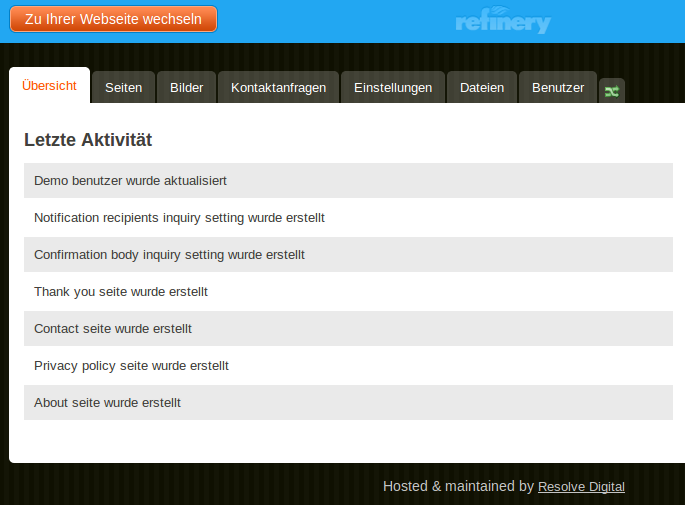
\includegraphics[scale=0.3]{images/analyse/refinery/backendrefinery.png}
\caption{Backend-Ansicht von Refinery CMS}
\label{refinerybackend}
\end{center}
\end{figure}

\begin{description}
\item[Übersichts-Modul]\mbox{~}\\*
Nach der Anmeldung am System bildet das Übersichts-Modul (o.a. Dashboard) die Startseite des Systems. Dort können in einer einfachen Form die letzten Aktivitäten innerhalb des CMS eingesehen werden. Zusätzlich werden Schnellaufrufe zu systemspezifischen Funktionen angeboten.
\item[Seiten-Modul]\mbox{~}\\*
Das Seiten-Modul listet alle angelegten Seiten und Unterseiten in Form einer Baumstruktur auf. Zusätzlich können Titel und Metainformationen bearbeitet werden. Die erstellten Seiten verfügen jeweils über einen oder mehrere WYSIWYG-Editor-Textfelder\footnote{Die einzelnen Inhaltsblöcke werden als Content Sections bezeichnet. Die Anzahl der pro Seite zur Verfügung stehenden Inhaltsblöcke kann beliebig festgelegt werden. Die Positionierung der einzelnen Blöcke wird durch ein zuvor festgelegtes HTML-Template im Rails-Quellcode festgelegt.}, in die der Inhalt der Seite eingepflegt werden kann (Abb. \ref{contentsections}).

\begin{figure}[!h]
\begin{center}
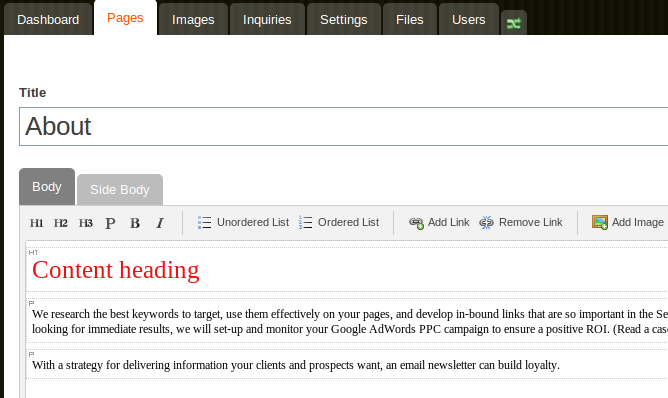
\includegraphics[scale=0.3]{images/analyse/refinery/contentsections.png}
\caption{Seitenbearbeitung in Refinery CMS mit geöffneten Content Sections Body und Site Body}
\label{contentsections}
\end{center}
\end{figure}
\item[Bilder- und Dateien-Modul]\mbox{~}\\*
In Refinery wird durch die Wahl der Menüpunkte Bilder und Dateien die Ressourcenverwaltung des Systems geöffnet. Dort können anschließend 	Mediendateien verschiedenster Formate hochgeladen, bearbeitet und durchsucht werden.
\item[Benutzer-Modul]\mbox{~}\\*
Das Benutzer-Modul erlaubt die Verwaltung der am System registrierten 	Anwender. U.a. können dort Nutzername, Passwort und Berechtigungen für die Verwendung anderer Module gesetzt werden.
\item[Einstellungs-Modul]\mbox{~}\\*
Die einzelnen Module und Erweiterungen von Refinery können durch zuvor definierte Parameter\footnote{Die offizielle Bezeichnung der Parameter lautet \emph{Refinery Settings}} in ihrem Verhalten oder Ausehen beeinflusst werden. Das Einstellungs-Modul listet die in einer CMS-Installation vorhandenen Konfigurationsoptionen auf und ermöglicht eine nachträgliche Editierung und Löschung dieser.
\end{description}
\subsection{Erweiterungen}
Erweiterungen werden in Refinery als Engines bezeichnet. Sie werden durch Aktivierung innerhalb der Rails-Anwendung (im Quellcode) installiert und anschließend im Benutzer-Modul von Refinery den einzelnen Anwendern zugeordnet. Zum Zeitpunkt der Erstellung dieser Arbeit existieren u.a. folgende Erweiterungen:
\begin{itemize}
\item
refinerycms-inquiries\footnote{Komponenten-Download: \href{https://github.com/resolve/refinerycms-inquiries}{https://github.com/resolve/refinerycms-inquiries}}: Darstellung von Kontaktanfragen auf der Internetseite mit zusätzlicher Verwaltungsfunktion der Anfragen im Backend von Refinery CMS
\item
refinerycms-news\footnote{Komponenten-Download: \href{https://github.com/resolve/refinerycms-news}{https://github.com/resolve/refinerycms-news}}: Verwaltung und Darstellung von Nachrichten im Front- und Backend-Bereich
\item
 refinerycms-blog\footnote{Komponenten-Download: \href{https://github.com/resolve/refinerycms-blog}{https://github.com/resolve/refinerycms-blog}}: Engine zur Erstellung kurzer Beiträge inklusive Kategorisierungs- und Kommentarfunktion
\end{itemize}

\subsection{Verwendete Technologien}
Refinery CMS ist ein technologisch sehr einfaches System. Die Realisierung der Backend-Funktionalitäten wird durch die konsequente Verwendung von HTML 5 erreicht. Zur Generierung der Dialoge, die u.a. innerhalb des Bild- und Dateien-Moduls eingesetzt werden, greift Refinery auf die jQuery UI Bibliothek zurück. Der im Seiten-Modul integrierte WYSIWYG-Editor ist ein für die Anforderungen des CMS angepasster, XHTML konformer JavaScript WYMeditor.
Durch die Unterstützung von HTML 5 innerhalb des Backend können Datenübertragungen von Medien an den Server in Form von Multi-Uploads realisiert werden. Die sonst übliche Nutzung von Flash entfällt und vereinfacht damit das System zusätzlich.
Die bereits angesprochenen Erweiterungen (Engines) sind eigenständige Rails-Anwendungen, deren Grundgerüst mit Hilfe eines Refinery-Engine-Generators erzeugt wird.
Die geringen technologischen Abhängigkeiten und Anforderungen des Systems erlauben es, Teile des Backends bei Bedarf anzupassen, zu verändern oder komplett auszutauschen.
%Refinery END


\section{Durchführung der funktionalen Analyse}
\label{sec:durchanalyse}
Um die Leistungsfähigkeit der ausgewählten Systeme im Bereich des Webpublishing einschätzen zu können, werden die vorgestellten Kriterien des vorhergehenden Abschnitts mit den ausgewählten WCMS in Tabellenform gegenübergestellt. Es erfolgt dabei eine Festlegung der Erfüllung dieser Kriterien in folgende 2 Stufen:

\begin{table}[!h]
\renewcommand{\arraystretch}{1.5}
\center
\caption{Mögliche Auswertungsstufen für die umgesetzten Funktionalitäten der WCMS}
\begin{tabular}{|l|p{10cm}|}
\hline
\cellcolor{green} Erfüllt 100\% & Das hier vorgestellte WCMS erfüllt die aus dem
Kriterium definierten Funktionalitäten. Dies kann auch durch Installation einer Zusatzkomponente erreicht werden.\\
\hline
\cellcolor{red} Erfüllt 0\% & Das hier vorgestellte WCMS erfüllt die aus dem
Kriterium definierten Funktionalitäten nicht. Es existieren darüber hinaus keine Erweiterungsmöglichkeiten für das System oder die Erfüllung ist nur durch eigenständige Implementierung (Programmierung) erreichbar.\\
\hline
\end{tabular}
\end{table}
Zusätzlich werden bei bestehenden Einschränkungen und Problemen zu jedem WCMS noch Erläuterungen aufgeführt, die eine genauere Einschätzung des tatsächlichen Funktionsumfangs liefern können.
\subsection{Erstellung}
\begin{tabular}[!ht]{|l|l|l|l|}
\hline
\multicolumn{4}{|p{15cm}|}{\textbf{Mehrere Benutzer sollen gleichzeitig Inhalte verwalten und erfassen können}} \\
\hline
  Alchemy 1.6.0 & \cellcolor{green}Erfüllt: 100\% & Refinery CMS 1.0.8 & \cellcolor{green}Erfüllt: 100\% \\
  \hline
  \multicolumn{2}{|p{7.5cm}|}{Nutzer und Administratoren können Inhalte gleichzeitig erfassen und verwalten.}
   & \multicolumn{2}{p{7.5cm}|}{Nutzer und Administratoren können Inhalte gleichzeitig erfassen und verwalten.} \\
  \hline
  Browser CMS 3.3.1 & \cellcolor{green}Erfüllt: 100\% & Locomotive CMS & \cellcolor{green}Erfüllt: 100\% \\
  \hline
  \multicolumn{2}{|p{7.5cm}|}{Nutzer und Administratoren können Inhalte gleichzeitig erfassen und verwalten.} & \multicolumn{2}{p{7.5cm}|}{Nutzer und Administratoren können Inhalte gleichzeitig erfassen und verwalten.} \\
\hline
\end{tabular}
\newline
\newline
\newline
\begin{tabular}[!ht]{|l|l|l|l|}
\hline
\multicolumn{4}{|p{15cm}|}{\textbf{Inhalte sollen – unabhängig von Zeit- und Standort – durch mehrere Benutzer online verwaltet und erfasst werden können}} \\
\hline
  Alchemy 1.6.0 & \cellcolor{green}Erfüllt: 100\% & Refinery CMS 1.0.8 & \cellcolor{green}Erfüllt: 100\% \\
  \hline
  \multicolumn{2}{|p{7.5cm}|}{Vollständig unterstützt} & \multicolumn{2}{p{7.5cm}|}{Vollständig unterstützt} \\
  \hline
  Browser CMS 3.3.1 & \cellcolor{green}Erfüllt: 100\% & Locomotive CMS & \cellcolor{green}Erfüllt: 100\% \\
  \hline
  \multicolumn{2}{|p{7.5cm}|}{Vollständig unterstützt} & \multicolumn{2}{p{7.5cm}|}{Vollständig unterstützt} \\
\hline
\end{tabular}
\newline
\newline
\newline
\begin{tabular}[!ht]{|l|l|l|l|}
\hline
\multicolumn{4}{|p{15cm}|}{\textbf{Offline Erfassung von Inhalten unter Verwendung eines lokal auf dem Rechner installierten Programms}} \\
\hline
  Alchemy 1.6.0 & \cellcolor{red}Erfüllt: 0\% & Refinery CMS 1.0.8 & \cellcolor{red}Erfüllt: 0\% \\
  \hline
  \multicolumn{2}{|p{7.5cm}|}{Wird nicht unterstützt} & \multicolumn{2}{p{7.5cm}|}{Wird nicht unterstützt} \\
  \hline
  Browser CMS 3.3.1 & \cellcolor{red}Erfüllt: 0\% & Locomotive CMS & \cellcolor{red}Erfüllt: 0\% \\
  \hline
  \multicolumn{2}{|p{7.5cm}|}{Wird nicht unterstützt} & \multicolumn{2}{p{7.5cm}|}{Wird nicht unterstützt} \\
\hline
\end{tabular}
\newline
\newline
\newline
\begin{tabular}[!ht]{|l|l|l|l|}
\hline
\multicolumn{4}{|p{15cm}|}{\textbf{Integrierte Mediendatenbank zur Erfassung und Verwaltung von Bildern, Multimedia,Texten, Audio, Videos, usw.}} \\
\hline
  Alchemy 1.6.0 & \cellcolor{green}Erfüllt: 100\% & Refinery CMS 1.0.8 & \cellcolor{green}Erfüllt: 100\% \\
  \hline
  \multicolumn{2}{|p{7.5cm}|}{Alchemy bietet eine Bibliothek, in der Bilder und Dateien verwaltet werden können.}
   & \multicolumn{2}{p{7.5cm}|}{Refinery CMS bietet eine einfache Medienverwaltung.} \\
  \hline
  Browser CMS 3.3.1 & \cellcolor{green}Erfüllt: 100\% & Locomotive CMS & \cellcolor{green}Erfüllt: 100\% \\
  \hline
  \multicolumn{2}{|p{7.5cm}|}{Browser CMS verfügt über eine \emph {Content Library}, die eine einfache Medienverwaltung von Bildern, Dateien und definierten Inhaltselementen ermöglicht.} & \multicolumn{2}{p{7.5cm}|}{Locomotive CMS bietet eine Asset-Verwaltung, in der selbst erstellte Inhaltselemente in Containern verwaltet werden können.} \\
\hline
\end{tabular}
\newline
\newline
\newline
\begin{tabular}[!ht]{|l|l|l|l|}
\hline
\multicolumn{4}{|p{15cm}|}{\textbf{Inhalte sollen ohne spezielle Programmier / HTML-Kenntnisse erfasst und verwaltet werden können}} \\
\hline
  Alchemy 1.6.0 & \cellcolor{green}Erfüllt: 100\% & Refinery CMS 1.0.8 & \cellcolor{green}Erfüllt: 100\% \\
  \hline
  \multicolumn{2}{|p{7.5cm}|}{Alle Inhalte können über den TinyMCE-Javascript WYSIWYG Editor erfasst und formatiert werden.}
   & \multicolumn{2}{p{7.5cm}|}{Alle Inhalte können über den integrierten WYSIWYG-Editor Wymeditor erfasst und formatiert werden. Der Editor ist fest in das System integriert und kann nicht ausgetauscht werden. Ein Plugin, dass die Verwendung eines anderen Editors ermöglicht ist bereits in Planung.} \\
  \hline
  Browser CMS 3.3.1 & \cellcolor{green}Erfüllt: 100\% & Locomotive CMS & \cellcolor{green}Erfüllt: 100\% \\
  \hline
  \multicolumn{2}{|p{7.5cm}|}{In Browser CMS findet der WYSIWIG-FCKEditor Verwendung. Zusätzlich stehen verschiedene Module zur Verfügung, die einen Austausch des Editors gegen andere Lösungen ermöglichen.} & \multicolumn{2}{p{7.5cm}|}{Alle Inhalte können über zwei integrierte WYSIWYG-Editoren erfasst und formatiert werden. Im Backend steht der Javascript Editor TinyMCE zur Verfügung. Im Frontend findet der HTML5-WYSIWYG-Editor Aloha zur Manipulierung der Seiteninhalte Verwendung (befindet sich noch in der Entwicklung).} \\
\hline
\end{tabular}
\newline
\newline
\newline
\begin{tabular}[!ht]{|l|l|l|l|}
\hline
\multicolumn{4}{|p{15cm}|}{\textbf{Inhalte sollen in einer Datenbank gespeichert werden}} \\
\hline
  Alchemy 1.6.0 & \cellcolor{green}Erfüllt: 100\% & Refinery CMS 1.0.8 & \cellcolor{green}Erfüllt: 100\% \\
  \hline
  \multicolumn{2}{|p{7.5cm}|}{Alchemy verwendet Active Record als Datenbankpersistenzschicht. Durch die Verwendung von Migrationen könen so eine Vielzahl relationaler Datenbanken unterstützt werden. Zusätzlich exisitieren einige Adapter, um auch dokumentenbasierte Datenbanken anzusteuern.}
   & \multicolumn{2}{p{7.5cm}|}{Refinery greift ebenfalls auf Rails' Active Record zurück und unterstützt damit mehrere relationale und dokumentenorientierte Datenbanken.} \\
  \hline
  Browser CMS 3.3.1 & \cellcolor{green}Erfüllt: 100\% & Locomotive CMS & \cellcolor{green}Erfüllt: 100\% \\
  \hline
  \multicolumn{2}{|p{7.5cm}|}{Wie bei Alchemy und Refinery CMS wird hier auch auf Active Record zurückgegriffen. Die Entwickler garantieren auf Grund fehlender Tests jedoch nur die Unterstützung von SQLite und MySQL-Datenbanken. Tendenziell können aber alle von Active Record unterstützten Datenbanken eingesetzt werden.} & \multicolumn{2}{p{7.5cm}|}{Locomotive CMS greift im Gegensatz zu seinen Konkurrenten auf die dokumentenorientierten Datenbank MongoDB zurück. Relationale Datenbanken werden somit nicht unterstützt. Eine Umsetzung von Locomotive mit Active Record ist jedoch geplant.} \\
\hline
\end{tabular}
\newline
\newline
\newline
\begin{tabular}[!ht]{|l|l|l|l|}
\hline
\multicolumn{4}{|p{15cm}|}{\textbf{Inhalte (Texte, Bilder, Videos etc.) sollen zentral kategorisiert, erfasst und verwaltet werden können}} \\
\hline
  Alchemy 1.6.0 & \cellcolor{red}Erfüllt: 0\% & Refinery CMS 1.0.8 & \cellcolor{red}Erfüllt: 0\% \\
  \hline
  \multicolumn{2}{|p{7.5cm}|}{Die Bibliothek von Alchemy unterstützt lediglich eine Auflistung von Resourcen. Bilder und Dateien können damit nur in Form einer Listenansicht inspiziert werden. Eine Zuordnung zu Kategorien oder eine Anlage von Ordnerstrukturen zur Erleichterung der Orientierung ist nicht möglich. Die Verwaltung großer Datenmengen scheint daher nur schwer möglich.}
   & \multicolumn{2}{p{7.5cm}|}{Ähnlich wie bei Alchemy gleicht die Resourcenverwaltung nur einer einfachen Auflistung von Bildern und anderen Ressourcen. Eine Kategorisierung der Inhalte ist nicht möglich. Ebenfalls können keine Ordner zur sinnvollen Strukturierung der Ressourcen erstellt werden. Die Verwaltung großer Datenmengen wird dadurch schnell zu einem Geduldsakt.} \\
  \hline
  Browser CMS 3.3.1 & \cellcolor{red}Erfüllt: 0\% & Locomotive CMS & \cellcolor{red}Erfüllt: 0\% \\
  \hline
  \multicolumn{2}{|p{7.5cm}|}{Die \emph{Content Library} von Browser CMS listet wie ihre Vorgänger lediglich die angelegten Bilder oder Dateien auf. Möglichkeiten zur sinnvollen Organisation (Kategorien, Ordner) großer Datenmengen sind nicht vorhanden.} & \multicolumn{2}{p{7.5cm}|}{Die Inhaltsverwaltung kann nicht kategorisiert werden. Wie bei seinen Vorgängern sind die Datensätze lediglich in Listenform aufgeführt. Eine logische Strukturierung mit Hilfe von Ordnern ist nicht möglich.} \\
\hline
\end{tabular}
\newline
\newline
\newline
\begin{tabular}[!ht]{|l|l|l|l|}
\hline
\multicolumn{4}{|p{15cm}|}{\textbf{Inhalte können während der Erfassung über eine Preview-Funktion vorab im Design der Webseite angesehen werden}} \\
\hline
  Alchemy 1.6.0 & \cellcolor{green}Erfüllt: 100\% & Refinery CMS 1.0.8 & \cellcolor{red}Erfüllt: 0\% \\
  \hline
  \multicolumn{2}{|p{7.5cm}|}{Redakteure können ihre erstellten und editierten Inhalte im Backend durch ein Preview-Fenster sichtbar machen. Änderungen an Inhaltselementen können somit sofort nachvollzogen werden.}
   & \multicolumn{2}{p{7.5cm}|}{Refinery CMS verfügt über keine Preview-Funktion der Inhalte. Ist ein Inhaltselement im Backend neu angelegt oder bearbeitet wurden, wird dies auf der Internetseite sofort sichtbar.} \\
  \hline
  Browser CMS 3.3.1 & \cellcolor{green}Erfüllt: 100\% & Locomotive CMS & \cellcolor{red}Erfüllt: 0\% \\
  \hline
  \multicolumn{2}{|p{7.5cm}|}{Wie bei Alchemy werden Inhalte erst nach ihrer Veröffentlichung sichtbar. Bis dahin kann jedoch im Frontend durch Inline-Editing der Seite jedes Inhaltselement bearbeitet werden.} & \multicolumn{2}{p{7.5cm}|}{Locomotive CMS bietet wie RefineryCMS keine Preview-Funktion. Änderungen und neu angelegte Inhalte werden direkt veröffentlicht.} \\
\hline
\end{tabular}
\newline
\newline
\newline
\begin{tabular}[!ht]{|l|l|l|l|}
\hline
\multicolumn{4}{|p{15cm}|}{\textbf{Zuordnung von standardisierten und frei definierbaren Metadaten zu Inhalten (z.B. Autor, Schlüsselwörter, Benutzerdefinierte Felder) soll möglich sein}} \\
\hline
  Alchemy 1.6.0 & \cellcolor{red}Erfüllt: 0\% & Refinery CMS 1.0.8 & \cellcolor{red}Erfüllt: 0\% \\
  \hline
  \multicolumn{2}{|p{7.5cm}|}{Metadaten zu Inhalten können nicht vergeben werden.}
   & \multicolumn{2}{p{7.5cm}|}{Inhalte werden als einfache Datensätze betrachtet und besitzen daher keine definierten Metadaten.} \\
  \hline
  Browser CMS 3.3.1 & \cellcolor{green}Erfüllt: 100\% & Locomotive CMS & \cellcolor{green}Erfüllt: 100\% \\
  \hline
  \multicolumn{2}{|p{7.5cm}|}{Metadaten können zu einzelnen Inhaltselementen in Form einer Tag-Liste hinzugefügt werden. Diese wird in der Datenbank als Text abgespeichert und bei ihrer Nutzung in einzelne Teil-Strings zerlegt. Das Hinzufügen zuvor definierter Metadaten ist nicht möglich.} & \multicolumn{2}{p{7.5cm}|}{Zu den verschiedenen Inhaltselementen können beliebig viele Metadaten hinzugefügt werden. Auch die Darstellung von 1:1 und 1:n-Beziehungen ist möglich. Diese Funktionalität wird dabei vor allem durch die Verwendung der dokumentenbasierten Datenbank MongoDB möglich.} \\
\hline
\end{tabular}
\newline
\newline
\newline
\begin{tabular}[!ht]{|l|l|l|l|}
\hline
\multicolumn{4}{|p{15cm}|}{\textbf{Inhalte sollen mehrsprachig erfasst und verwaltet werden können}} \\
\hline
  Alchemy 1.6.0 & \cellcolor{green}Erfüllt: 100\% & Refinery CMS 1.0.8 & \cellcolor{green}Erfüllt: 100\% \\
  \hline
  \multicolumn{2}{|p{7.5cm}|}{In Alchemy können Inhalte mehrsprachig angelegt werden. Durch die Auswahl einer bestimmten Sprache wird ein entsprechender Seitenbaum mit allen existierenden Inhalten zu der ausgewählten Sprache erzeugt.}
   & \multicolumn{2}{p{7.5cm}|}{Refinery CMS kann Inhalte mehrsprachig verwalten und ausgeben. Zur Aktivierung der Funktionalität müssen nur die zu unterstützenden Sprachen in einer Konfigurationsdatei angegeben werden (dies kann von Administtratoren im Backend vorgenommen werden). Alle Sprachen werden dabei in einem einzigen Seitenbaum verwaltet. Vorhandene Übersetzungen zu einer bestimmten Seite werden durch Einblendung von Flaggensymbolen kenntlich gemacht.} \\
  \hline
  Browser CMS 3.3.1 & \cellcolor{red}Erfüllt: 0\% & Locomotive CMS & \cellcolor{red}Erfüllt: 0\% \\
  \hline
  \multicolumn{2}{|p{7.5cm}|}{In Browser CMS kann  durch die Installation der Erweiterung \emph{browsercmsi} die Unterstützung von mehrsprachigen Inhalten erreicht werden. Der Plugin-Anbieter konnte die 100\% Rails 3-Kompatibilität der Erweiterung jedoch nicht garantieren. Von einem Einsatz dieser Lösung in einer Produktiv-Umgebung wird daher abgeraten. Innerhalb der Bewertung von Browser CMS werden daher 0\% beim Erfüllungsgrad angegeben.} & \multicolumn{2}{p{7.5cm}|}{Inhalte können nur einsprachig verwaltet werden. Erweiterungen, die diese Funktionalität herstellen können, konnten nicht ermittelt werden.} \\
\hline
\end{tabular}
\newline
\newline
\newline
\begin{tabular}[!ht]{|l|l|l|l|}
\hline
\multicolumn{4}{|p{15cm}|}{\textbf{Das CMS soll über eine offene API (Programmierschnittstelle) für individuelle Erweiterung verfügen}} \\
\hline
  Alchemy 1.6.0 & \cellcolor{green}Erfüllt: 100\% & Refinery CMS 1.0.8 & \cellcolor{green}Erfüllt: 100\% \\
  \hline
  \multicolumn{2}{|p{7.5cm}|}{Eine flexible Plugin-DSL (Domain Specific Language) erlaubt das Hinzufügen von individuellen Erweiterungen.}
   & \multicolumn{2}{p{7.5cm}|}{Individuelle Inhaltselemente können durch die Verwendung der Refinery Engine Generatoren hinzugefügt werden. Die weitere Entwicklung Anpassung des Codegerüst folgt dann mit den inenrhalb des Rails Framework üblichen Entwicklungstechniken und -abläufen.} \\
  \hline
  Browser CMS 3.3.1 & \cellcolor{green}Erfüllt: 100\% & Locomotive CMS & \cellcolor{green}Erfüllt: 100\% \\
  \hline
  \multicolumn{2}{|p{7.5cm}|}{Ähnlich wie bei Refinery CMS können neue Module und Inhaltstypen mit Hilfe von speziellen Rails-Generatoren erzeugt werden.} & \multicolumn{2}{p{7.5cm}|}{Neue Inhaltstypen lassen sich im Backend durch ein einfaches User-Interface zusammenstellen.  Mit wenigen Klicks sind so schnell neue Elemente erstellt. Programmierkenntnisse sind nicht notwendig.} \\
\hline
\end{tabular}
\newline
\newline
\newline
\begin{tabular}[!ht]{|l|l|l|l|}
\hline
\multicolumn{4}{|p{15cm}|}{\textbf{Für die Verwaltung und Erfassung von Inhalten sollen alle gängigen Internet-Browser (Internet Explorer, Safari und Firefox) eingesetzt werden können}} \\
\hline
  Alchemy 1.6.0 & \cellcolor{green}Erfüllt: 100\% & Refinery CMS 1.0.8 & \cellcolor{green}Erfüllt: 100\% \\
  \hline
  \multicolumn{2}{|p{7.5cm}|}{Vollständig unterstützt}
   & \multicolumn{2}{p{7.5cm}|}{Vollständig unterstützt} \\
  \hline
  Browser CMS 3.3.1 & \cellcolor{green}Erfüllt: 100\% & Locomotive CMS & \cellcolor{green}Erfüllt: 100\% \\
  \hline
  \multicolumn{2}{|p{7.5cm}|}{Vollständig unterstützt} & \multicolumn{2}{p{7.5cm}|}{Vollständig unterstützt} \\
\hline
\end{tabular}
\newline
\newline
\newline
\begin{tabular}[!ht]{|l|l|l|l|}
\hline
\multicolumn{4}{|p{15cm}|}{\textbf{Inhalte sollen einfach importiert / exportiert werden können - dabei kommen Formate wie z.B. XML zum Einsatz}} \\
\hline
  Alchemy 1.6.0 & \cellcolor{red}Erfüllt: 0\% & Refinery CMS 1.0.8 & \cellcolor{red}Erfüllt: 0\% \\
  \hline
  \multicolumn{2}{|p{7.5cm}|}{Alchemy verfügt über keine integrierten Import und Export-Funktionalitäten.}
   & \multicolumn{2}{p{7.5cm}|}{Es existieren auf Nutzerebene keine Möglichkeiten des Im- und Exports. Durch sogenannte Seed-Dateien ist jedoch ein nachträgliches Befüllen der Datenbank möglich. Der Aufruf erfordert jedoch Kenntnisse in Ruby on Rails und ist daher für Normalanwender/Redakteure nicht sinnvoll.} \\
  \hline
  Browser CMS 3.3.1 & \cellcolor{red}Erfüllt: 0\% & Locomotive CMS & \cellcolor{green}Erfüllt: 100\% \\
  \hline
  \multicolumn{2}{|p{7.5cm}|}{In Browser CMS können Inhalte nicht importiert und exportiert werden. Entsprechende Features müssten erst eigenständig implementiert werden.} & \multicolumn{2}{p{7.5cm}|}{In Locomotive CMS kann ein kompletter Internetauftritt mit seinen Inhalten und Ressourcen importiert und exportiert werden. Zum Austausch der Inhalte findet eine \emph{Zip}-Datei Verwendung, die alle benötigten Ressourcen (Bilder, Dateien, Templates usw.) sowie Inhalte der Datenbank einschließt. Ressourcen werden dabei in vordefinierten Ordnerstrukturen abgelegt. Die Datenbankeinträge aus MongoDB werden innerhalb der \emph{Zip}-Datei im Unterordner \emph{data} abgelegt. Die Einträge liegen dabei  im \emph{YAML}-Format vor.} \\
\hline
\end{tabular}
\newline
\newline
\newline
\begin{tabular}[!ht]{|l|l|l|l|}
\hline
\multicolumn{4}{|p{15cm}|}{\textbf{Integration von Inhalten anderer Webseiten, Multimedia, Applikationen, E-Commerce-Tools}} \\
\hline
  Alchemy 1.6.0 & \cellcolor{green}Erfüllt: 100\% & Refinery CMS 1.0.8 & \cellcolor{green}Erfüllt: 100\% \\
  \hline
  \multicolumn{2}{|p{7.5cm}|}{Der verwendete WYSIWYG-Editor \emph{TinyMCE} erlaubt in seiner HTML-Ansicht das Einbinden von Fremdinhalten anderer Seiten (z.B. IFrame). Zusätzlich ist die Erstellung von eigenen Inhaltselementen mit Hilfe der Alchemy Plugin DSL-API denkbar. So können auch die verschiedenen Resourcen aus der Bibliothek von Alchemy Verwendung finden. Standardmäßig verfügt Alchemy bereits über die Inhaltselemente \emph{Artikel}, \emph{Text}, \emph{Text mit Bild}, \emph{Bilder}, \emph{Bildergalerie}, \emph{Überschrift} und \emph{Intro}.}
   & \multicolumn{2}{p{7.5cm}|}{Refinery CMS verwaltet jede Internetseite innerhalb eines flexiblen WYSIWYG-Editors. Die Integration von vordefiniertem HTML-Code kann dabei durch Nutzung der HTML-Ansicht des Editors erreicht werden.
} \\
  \hline
  Browser CMS 3.3.1 & \cellcolor{green}Erfüllt: 100\% & Locomotive CMS & \cellcolor{green}Erfüllt: 100\% \\
  \hline
  \multicolumn{2}{|p{7.5cm}|}{Wie seine Vorgänger auch können innerhalb des WYSIWYG-Editors IFrames oder anderer HTML-Code eingebetet werden. Vordefinierte Inhaltselemente, die vorhandene Ressourcen aus der \emph{Content Library} einbinden können, müssen eigenhändig angelegt werden.} & \multicolumn{2}{p{7.5cm}|}{Wie bei Alchemy und Refinery CMS können innerhalb des  WYSIWYG-Editors HTML-Fragmente angegeben werden.} \\
\hline
\end{tabular}
\subsection{Kontrolle}
\begin{tabular}[!ht]{|l|l|l|l|}
\hline
\multicolumn{4}{|p{15cm}|}{\textbf{Granulares Rechte- und Rollenkonzept für Anwender}} \\
\hline
  Alchemy 1.6.0 & \cellcolor{red}Erfüllt: 0\% & Refinery CMS 1.0.8 & \cellcolor{red}Erfüllt: 0\% \\
  \hline
  \multicolumn{2}{|p{7.5cm}|}{In Alchemy existieren vordefinierte Rollen (Registriert, Author, Redakteur,Administrator). Das Anlegen weiterer Rollen zur besseren Differenzierung ist jedoch nicht möglich.}
   & \multicolumn{2}{p{7.5cm}|}{Refinery CMS besitzt kein Rechte- und Rollenkonzept. Dem Anwender kann lediglich der Zugang zu bestimmten Plugins erlaubt oder entzogen werden, um so den Funktionsumfang einzuschränken.} \\
  \hline
  Browser CMS 3.3.1 & \cellcolor{green}Erfüllt: 100\% & Locomotive CMS & \cellcolor{red}Erfüllt: 0\% \\
  \hline
  \multicolumn{2}{|p{7.5cm}|}{In Browser CMS wird in einer Standardinstallation zwischen den Rollen Gast, CMS Administrator und Content Editor unterschieden. Zusätzlich können weitere Backend-Gruppen angelegt werden.} & \multicolumn{2}{p{7.5cm}|}{Locomotive CMS besitzt ein einfaches Rechte- und Rollenkonzept. Es wird zwischen Administratoren, Designern und Autoren unterschieden. Das Anlegen weiterer Gruppen ist nicht möglich.} \\
\hline
\end{tabular}
\newline
\newline
\newline
\begin{tabular}[!ht]{|l|l|l|l|}
\hline
\multicolumn{4}{|p{15cm}|}{\textbf{Granulares Berechtigungskonzept für einzelne Inhalte, Bereiche, Webseiten}} \\
\hline
  Alchemy 1.6.0 & \cellcolor{red}Erfüllt: 0\% & Refinery CMS 1.0.8 & \cellcolor{red}Erfüllt: 0\% \\
  \hline
  \multicolumn{2}{|p{7.5cm}|}{Die in Alchemy vordefinierte Rollen Registriert, Author, Redakteur und Administrator bestimmen den Funktionsumfang eines Anwenders im Backend. Angelegte Inhalte können jedoch nicht einzelnen Nutzern zugeordnet werden.}
   & \multicolumn{2}{p{7.5cm}|}{Nutzer können alle Inhalte und Bereiche einer Webseite editieren, solange sie zur Nutzung des bestimmten Plugins berechtigt wurden.} \\
  \hline
  Browser CMS 3.3.1 & \cellcolor{red}Erfüllt: 0\% & Locomotive CMS & \cellcolor{red}Erfüllt: 0\% \\
  \hline
  \multicolumn{2}{|p{7.5cm}|}{ Der Zugriff auf bestimmte Seiten (Seitenbaumzweige)  kann eingeschränkt werden. Zusätzlich bietet Browser CMS ein Erstellen von Frontend-Nutzergruppen an, um so bestimmte Seiten des CMS nur exklusiv ausgewählten Nutzern zur Verfügung zu stellen. Die Zugriffsberechtigung auf installierte Plugins kann ebenfalls für jeden Nutzer individuell festgelegt werden. Leider ist es nicht möglich, einzelne Inhaltselemente für bestimmte Nutzer unzugänglich zu machen.} & \multicolumn{2}{p{7.5cm}|}{Der Zugriff auf Seiten und Inhalte kann nicht individuell gesteuert und beeinflusst werden. Besitzt ein Anwender das Recht zum Editieren und Anlegen von Inhalten (Nutzergruppe Redakteur), können alle Inhalte im gesamten CMS bearbeitet werden.} \\
\hline
\end{tabular}
\newline
\newline
\newline
\begin{tabular}[!ht]{|l|l|l|l|}
\hline
\multicolumn{4}{|p{15cm}|}{\textbf{Schutz vor gegenseitigem Überschreiben erfasster Inhalte durch Check in/ Check out-Mechanismen}} \\
\hline
  Alchemy 1.6.0 & \cellcolor{red}Erfüllt: 0\% & Refinery CMS 1.0.8 & \cellcolor{red}Erfüllt: 0\% \\
  \hline
  \multicolumn{2}{|p{7.5cm}|}{Wird nicht unterstützt} & \multicolumn{2}{p{7.5cm}|}{Wird nicht unterstützt} \\
  \hline
  Browser CMS 3.3.1 & \cellcolor{red}Erfüllt: 0\% & Locomotive CMS & \cellcolor{red}Erfüllt: 0\% \\
  \hline
  \multicolumn{2}{|p{7.5cm}|}{Wird nicht unterstützt. Die automatische Versionierung von Inhaltselementen erlaubt jedoch ein nachträgliches, manuelles Sichten und Zusammenfügen  verschiedener Versionen.} & \multicolumn{2}{p{7.5cm}|}{Wird nicht unterstützt} \\
\hline
\end{tabular}
\newline
\newline
\newline
\begin{tabular}[!ht]{|l|l|l|l|}
\hline
\multicolumn{4}{|p{15cm}|}{\textbf{Versionierung von Inhalten mit Möglichkeit zur Wiederherstellung vorhergehender Versionen}} \\
\hline
  Alchemy 1.6.0 & \cellcolor{red}Erfüllt: 0\% & Refinery CMS 1.0.8 & \cellcolor{red}Erfüllt: 0\% \\
  \hline
  \multicolumn{2}{|p{7.5cm}|}{Versionierung und Wiederherstellung von Inhalten wird nicht unterstüzt.} & \multicolumn{2}{p{7.5cm}|}{Versionierung und Wiederherstellung von Inhalten wird nicht unterstüzt.} \\
  \hline
  Browser CMS 3.3.1 & \cellcolor{green}Erfüllt: 100\% & Locomotive CMS & \cellcolor{red}Erfüllt: 0\% \\
  \hline
  \multicolumn{2}{|p{7.5cm}|}{Wird unterstützt} & \multicolumn{2}{p{7.5cm}|}{Versionierung und Wiederherstellung von Inhalten wird nicht unterstüzt.} \\
\hline
\end{tabular}
\newline
\newline
\newline
\begin{tabular}[!ht]{|l|l|l|l|}
\hline
\multicolumn{4}{|p{15cm}|}{\textbf{Mandantenfähigkeit: Mehrfachnutzung des Systems durch verschiedene Parteien mit kompletter Trennung der Daten und Benutzer}} \\
\hline
  Alchemy 1.6.0 & \cellcolor{red}Erfüllt: 0\% & Refinery CMS 1.0.8 & \cellcolor{red}Erfüllt: 0\% \\
  \hline
  \multicolumn{2}{|p{7.5cm}|}{Wird nicht unterstüzt} & \multicolumn{2}{p{7.5cm}|}{Wird nicht unterstüzt} \\
  \hline
  Browser CMS 3.3.1 & \cellcolor{red}Erfüllt: 0\% & Locomotive CMS & \cellcolor{red}Erfüllt: 0\% \\
  \hline
  \multicolumn{2}{|p{7.5cm}|}{Wird nicht unterstüzt} & \multicolumn{2}{p{7.5cm}|}{In Locomotive CMS können mehrere Internetauftritte gleichzeitig verwaltet werden. Eine Trennung der verschiedenen Nutzer und Daten wird jedoch nicht angeboten.} \\
\hline
\end{tabular}
\newline
\newline
\newline
\begin{tabular}[!ht]{|l|l|l|l|}
\hline
\multicolumn{4}{|p{15cm}|}{\textbf{Linküberprüfung: Automatische Prüfung der Gültigkeit von internen und externen Links mit Möglichkeit zur Korrektur bzw. Benachrichtigung definierter Personengruppen}} \\
\hline
  Alchemy 1.6.0 & \cellcolor{red}Erfüllt: 0\% & Refinery CMS 1.0.8 & \cellcolor{red}Erfüllt: 0\% \\
  \hline
  \multicolumn{2}{|p{7.5cm}|}{Wird nicht unterstüzt} & \multicolumn{2}{p{7.5cm}|}{Wird nicht unterstüzt} \\
  \hline
  Browser CMS 3.3.1 & \cellcolor{red}Erfüllt: 0\% & Locomotive CMS & \cellcolor{red}Erfüllt: 0\% \\
  \hline
  \multicolumn{2}{|p{7.5cm}|}{Wird nicht unterstüzt} & \multicolumn{2}{p{7.5cm}|}{Wird nicht unterstüzt} \\
\hline
\end{tabular}


\subsection{Freigabe}
\begin{tabular}[!ht]{|l|l|l|l|}
\hline
\multicolumn{4}{|p{15cm}|}{\textbf{Möglichkeit für \emph{nicht technische} User den Workflow zu kreieren, verwalten und zu ändern. Es soll dafür kein Scripting / Programming notwendig sein}} \\
\hline
  Alchemy 1.6.0 & \cellcolor{red}Erfüllt: 0\% & Refinery CMS 1.0.8 & \cellcolor{red}Erfüllt: 0\% \\
  \hline
  \multicolumn{2}{|p{7.5cm}|}{Nutzer können in Alchemy keinen Workflowprozess kreieren. Es ist jedoch möglich, das Redakteure die von Autoren durchgeführten Änderungen kontrollieren und anschließend veröffentlichen.
Ein Austausch zwischen beiden Nutzergruppen ist nicht möglich (z.B. kurze Mitteilung an den Redakteur). Redakteure müssen so Änderungen der Seiteninhalte selbst erkennen.} & \multicolumn{2}{p{7.5cm}|}{Wird nicht unterstüzt} \\
  \hline
  Browser CMS 3.3.1 & \cellcolor{red}Erfüllt: 0\% & Locomotive CMS & \cellcolor{red}Erfüllt: 0\% \\
  \hline
  \multicolumn{2}{|p{7.5cm}|}{Ein Workflowprozess kann in Browser CMS nicht erzeugt werden. Autoren ist es nur möglich, ihre durchgeführten Änderungen an andere Backend-Nutzer mit Veröffentlichungsrechten weiterzuleiten (Simulierung eines einfachsten Workflows).} & \multicolumn{2}{p{7.5cm}|}{Wird nicht unterstüzt} \\
\hline
\end{tabular}
\begin{tabular}[!ht]{|l|l|l|l|}
\hline
\multicolumn{4}{|p{15cm}|}{\textbf{Definition von Workflows inkl. mehrstufiger Freigabeprozesse für die Freischaltung von Inhalten}} \\
\hline
  Alchemy 1.6.0 & \cellcolor{red}Erfüllt: 0\% & Refinery CMS 1.0.8 & \cellcolor{red}Erfüllt: 0\% \\
  \hline
  \multicolumn{2}{|p{7.5cm}|}{Wird nicht unterstüzt} & \multicolumn{2}{p{7.5cm}|}{Wird nicht unterstüzt} \\
  \hline
  Browser CMS 3.3.1 & \cellcolor{red}Erfüllt: 0\% & Locomotive CMS & \cellcolor{red}Erfüllt: 0\% \\
  \hline
  \multicolumn{2}{|p{7.5cm}|}{Wird nicht unterstüzt} & \multicolumn{2}{p{7.5cm}|}{Wird nicht unterstüzt} \\
\hline
\end{tabular}
\newline
\newline
\newline
\begin{tabular}[!ht]{|l|l|l|l|}
\hline
\multicolumn{4}{|p{15cm}|}{\textbf{Möglichkeit externe Benutzer in Workflows mit einbinden zu können}} \\
\hline
  Alchemy 1.6.0 & \cellcolor{red}Erfüllt: 0\% & Refinery CMS 1.0.8 & \cellcolor{red}Erfüllt: 0\% \\
  \hline
  \multicolumn{2}{|p{7.5cm}|}{Wird nicht unterstützt} & \multicolumn{2}{p{7.5cm}|}{Wird nicht unterstüzt} \\
  \hline
  Browser CMS 3.3.1 & \cellcolor{red}Erfüllt: 0\% & Locomotive CMS & \cellcolor{red}Erfüllt: 0\% \\
  \hline
  \multicolumn{2}{|p{7.5cm}|}{Wird nicht unterstützt} & \multicolumn{2}{p{7.5cm}|}{Wird nicht unterstüzt} \\
\hline
\end{tabular}
\newline
\newline
\newline
\begin{tabular}[!ht]{|l|l|l|l|}
\hline
\multicolumn{4}{|p{15cm}|}{\textbf{Unternehmensspezifische Bearbeitungsprozesse von Inhalten sollen über frei definierbare Workflows verwaltet werden können}} \\
\hline
  Alchemy 1.6.0 & \cellcolor{red}Erfüllt: 0\% & Refinery CMS 1.0.8 & \cellcolor{red}Erfüllt: 0\% \\
  \hline
  \multicolumn{2}{|p{7.5cm}|}{Wird nicht unterstützt} & \multicolumn{2}{p{7.5cm}|}{Wird nicht unterstüzt} \\
  \hline
  Browser CMS 3.3.1 & \cellcolor{red}Erfüllt: 0\% & Locomotive CMS & \cellcolor{red}Erfüllt: 0\% \\
  \hline
  \multicolumn{2}{|p{7.5cm}|}{Wird nicht unterstützt} & \multicolumn{2}{p{7.5cm}|}{Wird nicht unterstüzt} \\
\hline
\end{tabular}

\subsection{Publikation}
\begin{tabular}[!ht]{|l|l|l|l|}
\hline
\multicolumn{4}{|p{15cm}|}{\textbf{Trennung von Inhalt und Design unter Verwendung von Templates}} \\
\hline
  Alchemy 1.6.0 & \cellcolor{green}Erfüllt: 100\% & Refinery CMS 1.0.8 & \cellcolor{green}Erfüllt: 100\% \\
  \hline
  \multicolumn{2}{|p{7.5cm}|}{Inhalt und Design werden in Alchemy durch die Verwendung von \emph{erb}-Templates getrennt. Das Haupt-Template der Seite wird zu Beginn der Entwicklung von einem Designer festgelegt und anschließend in der Anwendung verankert (als fixe Ressource im Rails Quellcode). So können Redakteure das Aussehen der Internetseite nicht beeinflussen.} & \multicolumn{2}{p{7.5cm}|}{Wie Alchemy verwendet Refinery CMS \emph{erb} als Template-Sprache.
Trotz der so erreichten Trennung zwischen Inhalten und Design erschwert die fehlende Möglichkeit der Anpassung im Backend den Umgang mit dem gesamten WCMS. Dies gilt für das Haupttemplate der Seite sowie für alle Erweiterungen.} \\
  \hline
  Browser CMS 3.3.1 & \cellcolor{green}Erfüllt: 100\% & Locomotive CMS & \cellcolor{green}Erfüllt: 100\% \\
  \hline
  \multicolumn{2}{|p{7.5cm}|}{Browser CMS unterstützt die Verwendung verschiedener Template-Sprachen.
In einer Standard-Installation werden u.a. \emph{erb}, \emph{rjs} und \emph{rxml} angeboten.} & \multicolumn{2}{p{7.5cm}|}{In Locomotive CMS kann für jede Seite ein Template angegeben werden. Die dabei verwendete Templatesprache ist \emph{Liquid}.} \\
\hline
\end{tabular}
\newline
\newline
\newline
\begin{tabular}[!ht]{|l|l|l|l|}
\hline
\multicolumn{4}{|p{15cm}|}{\textbf{Mehrfachverwendung von Inhalten an verschiedenen Stellen mit unterschiedlichem Layout}} \\
\hline
  Alchemy 1.6.0 & \cellcolor{green}Erfüllt: 100\% & Refinery CMS 1.0.8 & \cellcolor{red}Erfüllt: 0\% \\
  \hline
  \multicolumn{2}{|p{7.5cm}|}{Inhaltselemente und Seiten können in Alchemy kopiert und wiederverwendet werden. Die Zuordnung eines neuen Templates muss durch den Administrator erfolgen (Änderung am Rails-Quellcode).} & \multicolumn{2}{p{7.5cm}|}{Inhalte und Seiten können nicht kopiert und mehrfach verwendet werden.} \\
  \hline
  Browser CMS 3.3.1 & \cellcolor{red}Erfüllt: 0\% & Locomotive CMS & \cellcolor{red}Erfüllt: 0\% \\
  \hline
  \multicolumn{2}{|p{7.5cm}|}{Es können nur Inhalte mehrfach verwendet werden.} & \multicolumn{2}{p{7.5cm}|}{In Locomotive CMS kann nur für jede Seite ein neues Template angegeben werden. Inhalte sind den einzelnen Seiten zugeordnet und nur dort verwendbar.} \\
\hline
\end{tabular}
\newline
\newline
\newline
\begin{tabular}[!ht]{|l|l|l|l|}
\hline
\multicolumn{4}{|p{15cm}|}{\textbf{Navigationsstrukturen werden automatisch vom CMS generiert, publiziert und verwaltet}} \\
\hline
  Alchemy 1.6.0 & \cellcolor{green}Erfüllt: 100\% & Refinery CMS 1.0.8 & \cellcolor{green}Erfüllt: 100\% \\
  \hline
  \multicolumn{2}{|p{7.5cm}|}{Wird unterstützt} & \multicolumn{2}{p{7.5cm}|}{Wird unterstützt} \\
  \hline
  Browser CMS 3.3.1 & \cellcolor{green}Erfüllt: 100\% & Locomotive CMS & \cellcolor{green}Erfüllt: 100\% \\
  \hline
  \multicolumn{2}{|p{7.5cm}|}{Wird unterstützt} & \multicolumn{2}{p{7.5cm}|}{Wird unterstützt} \\
\hline
\end{tabular}
\newline
\newline
\newline
\begin{tabular}[!ht]{|l|l|l|l|}
\hline
\multicolumn{4}{|p{15cm}|}{\textbf{Barrierefreiheit bei den publizierten Seiten soll unterstützt werden}} \\
\hline
  Alchemy 1.6.0 & \cellcolor{green}Erfüllt: 100\% & Refinery CMS 1.0.8 & \cellcolor{green}Erfüllt: 100\% \\
  \hline
  \multicolumn{2}{|p{7.5cm}|}{Barrierefreiheit kann bei entsprechender Umsetzung der Verwendeten Templates und CSS-Dateien erreicht werden.} & \multicolumn{2}{p{7.5cm}|}{Barrierefreiheit kann bei entsprechender Umsetzung der Verwendeten Templates und CSS-Dateien erreicht werden.} \\
  \hline
  Browser CMS 3.3.1 & \cellcolor{green}Erfüllt: 100\% & Locomotive CMS & \cellcolor{green}Erfüllt: 100\% \\
  \hline
  \multicolumn{2}{|p{7.5cm}|}{Barrierefreiheit kann bei entsprechender Umsetzung der Verwendeten Templates und CSS-Dateien erreicht werden.} & \multicolumn{2}{p{7.5cm}|}{Barrierefreiheit kann bei entsprechender Umsetzung der Verwendeten Templates und CSS-Dateien erreicht werden.} \\
\hline
\end{tabular}
\newline
\newline
\newline
\begin{tabular}[!ht]{|l|l|l|l|}
\hline
\multicolumn{4}{|p{15cm}|}{\textbf{Inhalte sollen auf verschiedene Medien / Technologien (Cross Media Publishing, SMS /Mobile / WAP / usw.) ausgegeben werden können}} \\
\hline
  Alchemy 1.6.0 & \cellcolor{red}Erfüllt: 0\% & Refinery CMS 1.0.8 & \cellcolor{red}Erfüllt: 0\% \\
  \hline
  \multicolumn{2}{|p{7.5cm}|}{Wird nicht unterstützt} & \multicolumn{2}{p{7.5cm}|}{Wird nicht unterstützt} \\
  \hline
  Browser CMS 3.3.1 & \cellcolor{red}Erfüllt: 0\% & Locomotive CMS & \cellcolor{red}Erfüllt: 0\% \\
  \hline
  \multicolumn{2}{|p{7.5cm}|}{Wird nicht unterstützt} & \multicolumn{2}{p{7.5cm}|}{Wird nicht unterstützt} \\
\hline
\end{tabular}
\newline
\newline
\newline
\begin{tabular}[!ht]{|l|l|l|l|}
\hline
\multicolumn{4}{|p{15cm}|}{\textbf{Möglichkeit Inhalte für anderen Webseiten bereitzustellen (XML, Webservice)}} \\
\hline
  Alchemy 1.6.0 & \cellcolor{red}Erfüllt: 0\% & Refinery CMS 1.0.8 & \cellcolor{green}Erfüllt: 100\% \\
  \hline
  \multicolumn{2}{|p{7.5cm}|}{Wird nicht unterstützt} & \multicolumn{2}{p{7.5cm}|}{Es gibt Plugins mit optionaler Ausgabe als RSS-Feed oder XML. Eine Bereitstellung ausgewählter Inhalte ist damit möglich.} \\
  \hline
  Browser CMS 3.3.1 & \cellcolor{green}Erfüllt: 100\% & Locomotive CMS & \cellcolor{red}Erfüllt: 0\% \\
  \hline
  \multicolumn{2}{|p{7.5cm}|}{Die Darstellung von Inhalten als RSS-Feeds ist möglich. Es muss jedoch selbst eingerichtet werden.} & \multicolumn{2}{p{7.5cm}|}{Wird nicht unterstützt} \\
\hline
\end{tabular}
\newline
\newline
\newline
\begin{tabular}[!ht]{|l|l|l|l|}
\hline
\multicolumn{4}{|p{15cm}|}{\textbf{Möglichkeit zur Wahl zwischen dynamischer oder statischer Generierung der Seiten / Inhalte}} \\
\hline
  Alchemy 1.6.0 & \cellcolor{red}Erfüllt: 0\% & Refinery CMS 1.0.8 & \cellcolor{red}Erfüllt: 0\% \\
  \hline
  \multicolumn{2}{|p{7.5cm}|}{Wird nicht unterstützt} & \multicolumn{2}{p{7.5cm}|}{Wird nicht unterstützt} \\
  \hline
  Browser CMS 3.3.1 & \cellcolor{green}Erfüllt: 100\% & Locomotive CMS & \cellcolor{red}Erfüllt: 0\% \\
  \hline
  \multicolumn{2}{|p{7.5cm}|}{Wird unterstützt} & \multicolumn{2}{p{7.5cm}|}{Wird nicht unterstützt} \\
\hline
\end{tabular}
\newline
\newline
\newline
\begin{tabular}[!ht]{|l|l|l|l|}
\hline
\multicolumn{4}{|p{15cm}|}{\textbf{Einfache Einbindung von Fremdinhalten welche durch Drittanbieter zur Verfügung gestellt werden}} \\
\hline
  Alchemy 1.6.0 & \cellcolor{green}Erfüllt: 100\% & Refinery CMS 1.0.8 & \cellcolor{green}Erfüllt: 100\% \\
  \hline
  \multicolumn{2}{|p{7.5cm}|}{Über den integrierten WYSIWYG-Editor können HTML-Fragmente eingebunden werden.} & \multicolumn{2}{p{7.5cm}|}{Über den integrierten WYSIWYG-Editor können HTML-Fragmente eingebunden werden.} \\
  \hline
  Browser CMS 3.3.1 & \cellcolor{green}Erfüllt: 100\% & Locomotive CMS & \cellcolor{green}Erfüllt: 100\% \\
  \hline
  \multicolumn{2}{|p{7.5cm}|}{Über den integrierten WYSIWYG-Editor können HTML-Fragmente eingebunden werden.} & \multicolumn{2}{p{7.5cm}|}{Über den integrierten WYSIWYG-Editor können HTML-Fragmente eingebunden werden.} \\
\hline
\end{tabular}
\newline
\newline
\newline
\begin{tabular}[!ht]{|l|l|l|l|}
\hline
\multicolumn{4}{|p{15cm}|}{\textbf{Automatisches Anbieten von Druckversion und Weiterempfehlen einer Webseite}} \\
\hline
  Alchemy 1.6.0 & \cellcolor{red}Erfüllt: 0\% & Refinery CMS 1.0.8 & \cellcolor{red}Erfüllt: 0\% \\
  \hline
  \multicolumn{2}{|p{7.5cm}|}{Wird nicht unterstützt} & \multicolumn{2}{p{7.5cm}|}{Wird nicht unterstützt} \\
  \hline
  Browser CMS 3.3.1 & \cellcolor{red}Erfüllt: 0\% & Locomotive CMS & \cellcolor{red}Erfüllt: 0\% \\
  \hline
  \multicolumn{2}{|p{7.5cm}|}{Wird nicht unterstützt} & \multicolumn{2}{p{7.5cm}|}{Wird nicht unterstützt} \\
\hline
\end{tabular}
\subsection{Terminierung/Archivierung}
\begin{tabular}[!ht]{|l|l|l|l|}
\hline
\multicolumn{4}{|p{15cm}|}{\textbf{Freie Wahl des Publikationszeitraumes (zeitgesteuertes Auf- / Abschalten / Archivieren) von Inhalten}} \\
\hline
  Alchemy 1.6.0 & \cellcolor{red}Erfüllt: 0\% & Refinery CMS 1.0.8 & \cellcolor{red}Erfüllt: 0\% \\
  \hline
  \multicolumn{2}{|p{7.5cm}|}{Wird nicht unterstützt} & \multicolumn{2}{p{7.5cm}|}{Wird nicht unterstützt} \\
  \hline
  Browser CMS 3.3.1 & \cellcolor{red}Erfüllt: 0\% & Locomotive CMS & \cellcolor{red}Erfüllt: 0\% \\
  \hline
  \multicolumn{2}{|p{7.5cm}|}{Wird nicht unterstützt} & \multicolumn{2}{p{7.5cm}|}{Wird nicht unterstützt} \\
\hline
\end{tabular}
\newline
\newline
\newline
\begin{tabular}[!ht]{|l|l|l|l|}
\hline
\multicolumn{4}{|p{15cm}|}{\textbf{Inhalte sollen archiviert werden können.}} \\
\hline
  Alchemy 1.6.0 & \cellcolor{red}Erfüllt: 0\% & Refinery CMS 1.0.8 & \cellcolor{red}Erfüllt: 0\% \\
  \hline
  \multicolumn{2}{|p{7.5cm}|}{Wird nicht unterstützt} & \multicolumn{2}{p{7.5cm}|}{Wird nicht unterstützt} \\
  \hline
  Browser CMS 3.3.1 & \cellcolor{red}Erfüllt: 0\% & Locomotive CMS & \cellcolor{red}Erfüllt: 0\% \\
  \hline
  \multicolumn{2}{|p{7.5cm}|}{Refinery CMS erlaubt das Archivieren von kompletten Seiten. Es ist jedoch nicht möglich, bestimmte Inhalte zu Archivieren.} & \multicolumn{2}{p{7.5cm}|}{Wird nicht unterstützt} \\
\hline
\end{tabular}





\newpage
\section{Auswertung der Ergebnisse}

Der Erfüllungsgrad der einzelnen Kriterien hat für die untersuchten WCMS folgendes Gesamtergebnis herausgestellt:

\begin{table}[!h]
\renewcommand{\arraystretch}{1.5}
%\small\addtolength{\tabcolsep}{+5pt}
\center
\begin{tabular}{|l|c|c|c|c|c|}
\hline
& & \multicolumn{4}{c|}{\textbf{Web Content Management System}} \\[2pt]
\cline{3-6}
\textbf{Bereich}& \textbf{Maximum} &
\begin{sideways}
Alchemy CMS
\end{sideways}
&\begin{sideways}
Browser CMS
\end{sideways}
&\begin{sideways}
Locomotive CMS
\end{sideways}
&\begin{sideways}
Refinery CMS
\end{sideways} \\
\hline
Erstellung & 1400 & 1000 & 1000 & 1000 & 900 \\
\hline
Kontrolle & 600 & 0 & 200 & 0 & 0 \\
\hline
Freigabe & 400 & 0 & 0 & 0 & 0 \\
\hline
Publikation & 1000 & 500 & 600 & 400 & 500 \\
\hline
Terminierung/Archivierung & 200 & 0 & 0 & 0 & 0 \\
\hline
\hline
Gesamtpunkte & 3600 & 1500 & 1800 & 1400 & 1400 \\
\hline
\end{tabular}
\end{table}


Die untersuchten Systeme zeigen bei der Erfüllung der für Webpublishing relevanten Kriterien sehr unterschiedliche Resultate. Im Bereich der Inhaltserstellung vefügen die Systeme über solide Funktionalitäten. Die Webpublishingbereiche Freigabe, Kontrolle und Terminierung/Archivierung decken dagegen bei allen untersuchten Systemen funktionale Deffizite auf. In der Gesamtbetrachtung liefert Browser CMS das beste Gesamtergebnis. Vor allem durch die umfassendere Nutzer- und Rechteverwaltung kann sich das System von Alchemy CMS und Locomotive CMS absetzen, die funktional gesehen im Mittelfeld angesiedelt sind. Refinery CMS besitzt auf Grund der fehlenden Inhalts- und Rechteverwaltung die geringsten Funktionalitäten aller Systeme.
\newline
Für einen besseren Gesamtüberblick werden die Ergebnisse der durchgeführten Analyse (Kaiptel \ref{sec:durchanalyse}) für jedes System noch einmal in einer Übersicht zusammengefasst.


\subsubsection{Alchemy CMS}

\begin{description}
\item[\emph{Erstellung}]\mbox{~}\\*
\begin{itemize}
	\item Umfassende Möglichkeiten zur Erstellung und Verwaltung von Seiten und verschiedenen Inhaltselementen in verschiedenen Sprachen
	\item Template-Erstellung und -verwaltung findet im Quellcode der Rails-Anwendung statt
	\item Umsetzung komplexer Seitenlayouts möglich
\end{itemize}
\item[\emph{Kontrolle}]\mbox{~}\\*
\begin{itemize}
	\item eingeschränkte Rechteverwaltung mit festgelegten Gruppen für Front- und Backend (Registriert, Author, Redakteur, Administrator)
	\item kein umfassendes Linkmanagement
\end{itemize}
\item[\emph{Freigabe}]\mbox{~}\\*
\begin{itemize}
	\item Einfacher Freigabeprozess für Internetseiten und Inhalte
	\item keine umfassende Workflowfunktionalität
\end{itemize}
\item[\emph{Publikation}]\mbox{~}\\*
\begin{itemize}
	\item Trennung der Inhalte vom Design durch Verwendung von Templates
	\item umfassende Seiten- und Inhaltsverwaltung mit Möglichkeiten zum Kopieren und Verschieben der Inhalte (Zwischenablagefunktion)
\end{itemize}
\item[\emph{Terminierung/Archivierung}]\mbox{~}\\*
\begin{itemize}
	\item Seiten und Inhalte können nicht archiviert oder zeitraumgebunden veröffentlicht werden
\end{itemize}
\end{description}

\newpage
\subsubsection{Browser CMS}

\begin{description}
\item[\emph{Erstellung}]\mbox{~}\\*
\begin{itemize}
	\item Umfassende Möglichkeiten zur Erstellung und Verwaltung von einsprachigen Seiten und verschiedenen Inhaltselementen
	\item Template-Erstellung und -verwaltung im Backend der Anwendung
	\item Umsetzung komplexer Seitenlayouts möglich
\end{itemize}
\item[\emph{Kontrolle}]\mbox{~}\\*
\begin{itemize}
	\item Rechteverwaltung mit vordefinierten Gruppen für Front- und Backend sowie Möglichkeiten zum Erstellen eigener Gruppen
	\item kein umfassendes Linkmanagement
\end{itemize}
\item[\emph{Freigabe}]\mbox{~}\\*
\begin{itemize}
	\item Einfacher Freigabeprozess für Internetseiten und Inhalte
	\item keine umfassende Workflowfunktionalität
\end{itemize}
\item[\emph{Publikation}]\mbox{~}\\*
\begin{itemize}
	\item Trennung der Inhalte vom Design durch Verwendung verschiedener Template-Sprachen
	\item Wiederverwendung von Inhaltenselementen
\end{itemize}
\item[\emph{Terminierung/Archivierung}]\mbox{~}\\*
\begin{itemize}
	\item Archivierung von erstellten Seiten
	\item keine zeitraumgebundene Veröffentlichung von Seiten und Inhalten möglich
\end{itemize}
\end{description}


\newpage
\subsubsection{Locomotive CMS}

\begin{description}
\item[\emph{Erstellung}]\mbox{~}\\*
\begin{itemize}
	\item Umfassende Möglichkeiten zur Erstellung und Verwaltung von einsprachigen Seiten und verschiedenen Inhaltselementen
	\item Inhaltselemente können im Backend der Seite individuell erstellt werden
	\item Umsetzung komplexe Layouts mit verschiedenen Seiten- und Inhaltselementen möglich
\end{itemize}
\item[\emph{Kontrolle}]\mbox{~}\\*
\begin{itemize}
	\item eingeschränkte Rechteverwaltung mit vordefinierten Gruppen für das Backend
	\item kein umfassendes Linkmanagement
\end{itemize}
\item[\emph{Freigabe}]\mbox{~}\\*
\begin{itemize}
	\item keine Abbildung von Freigabeprozessen für Internetseiten und Inhalte möglich
	\item keine Workflowfunktionalität
\end{itemize}
\item[\emph{Publikation}]\mbox{~}\\*
\begin{itemize}
	\item Trennung der Inhalte vom Design durch Verwendung der Template-Sprache Liquid
	\item Wiederverwendung von Inhaltenselementen
	\item eingeschränkte Möglichkeiten zum Verschieben
\end{itemize}
\item[\emph{Terminierung/Archivierung}]\mbox{~}\\*
\begin{itemize}
	\item Archivierung und Terminierung von Inhalten und Seiten ist nicht möglich
\end{itemize}
\end{description}

\subsubsection{Refinery CMS}

\begin{description}
\item[\emph{Erstellung}]\mbox{~}\\*
\begin{itemize}
	\item Erstellung und Verwaltung von mehrsprachigen Seiten und Inhaltsböcken
	\item Inhaltselemente können im Backend der Seite individuell erstellt werden
	\item Umsetzung komplexe Layouts mit Hilfe von Rails Views möglich
\end{itemize}
\item[\emph{Kontrolle}]\mbox{~}\\*
\begin{itemize}
	\item keine Rechteverwaltung für Seiten, Inhalte und Nutzer
	\item kein umfassendes Linkmanagement
\end{itemize}
\item[\emph{Freigabe}]\mbox{~}\\*
\begin{itemize}
	\item keine Unterstützung von Freigabeprozessen
	\item Erstellte Seiten können in den Bearbeitungsmodus gesetzt werden  und sind dadurch nicht mehr erreichbar
	\item keine Workflowfunktionalität
\end{itemize}
\item[\emph{Publikation}]\mbox{~}\\*
\begin{itemize}
	\item Trennung der Inhalte vom Design durch Verwendung der in Rails üblichen ERB-Views
	\item keine Wiederverwendung von Inhaltenselementen möglich
	\item keine Möglichkeiten zum Verschieben und Kopieren von Inhalten
\end{itemize}
\item[\emph{Terminierung/Archivierung}]\mbox{~}\\*
\begin{itemize}
	\item Archivierung und Terminierung von Inhalten und Seiten ist nicht möglich
\end{itemize}
\end{description}



\chapter{Beschreibung ausgewählter Implementierungsdetails}
\label{chap:probleme}
In diesem Abschnitt der Arbeit werden die ausgewählten Systeme hinsichtlich ihrer technischen Umsetzung mit dem Rails-Framework untersucht. Bei der Betrachtung wird auf folgende Aspekte eingegangen:

\begin{enumerate}
\item Wartbarkeit der Erweiterungen
\item Nutzeroberfläche
\end{enumerate}


\section{Erweiterungen}
\label{dryverstoss}
Innerhalb des Rails Frameworks ist die Verwendung von Generatoren ein häufiges Mittel zur schnellen Entwicklung von funktionsfähigem Code (siehe Kapitel \ref{sec:railsgeneratoren} ). Drei der vier hier vorgestellten Systeme\footnote{Locomotive CMS benötigt durch die Verwendung von MongoDB und der Möglichkeit, individuelle Inhaltselemente im Backend zu erstellen keine installierbaren Erweiterungsmodule} bedienen sich zur Realisierung neuer Inhaltslemente ebenfalls eines Generatorskripts, der ein für das jeweilige CMS funktionsbereites Grundgerüst erzeugt. Exemplarisch soll hier das Ergebnis eines Generatoraufrufes in Refinery CMS aufgezeigt werden (Abb. \ref{sec.refineryoutput} ). Das erstellte Inhaltselement Projekt verfügt dabei über die Felder Titel und Beschreibung:


%\lstinputlisting[numbers=none, caption=Aufruf des Refinery Engine Generators mit Ausgabe des erzeugten Codegerüsts, label=refinerygenerator]{code/generator_refinery.rb}

\begin{lstlisting}[label=sec.refineryoutput,caption=Aufruf des Refinery Engine Generators mit Ausgabe des erzeugten Codegerüsts]
rails generate refinery_engineproject name:string description:text
create  vendor/engines/projects/app/controllers/admin/projects_controller.rb
create  vendor/engines/projects/app/controllers/projects_controller.rb
create  vendor/engines/projects/app/models/project.rb
create  vendor/engines/projects/app/views/admin/projects/_actions.html.erb
create  vendor/engines/projects/app/views/admin/projects/_form.html.erb
create  vendor/engines/projects/app/views/admin/projects/_projects.html.erb
create  vendor/engines/projects/app/views/admin/projects/_records.html.erb
create  vendor/engines/projects/app/views/admin/projects/_project.html.erb
create  vendor/engines/projects/app/views/admin/projects/_sortable_list.html.erb
create  vendor/engines/projects/app/views/admin/projects/edit.html.erb
create  vendor/engines/projects/app/views/admin/projects/index.html.erb
create  vendor/engines/projects/app/views/admin/projects/new.html.erb
create  vendor/engines/projects/app/views/projects/index.html.erb
create  vendor/engines/projects/app/views/projects/show.html.erb
create  vendor/engines/projects/config/locales/en.yml
create  vendor/engines/projects/config/locales/fr.yml
create  vendor/engines/projects/config/locales/lolcat.yml
create  vendor/engines/projects/config/locales/nb.yml
create  vendor/engines/projects/config/locales/nl.yml
create  vendor/engines/projects/config/routes.rb
create  vendor/engines/projects/db/migrate/create_projects.rb
create  vendor/engines/projects/db/seeds/projects.rb
create  vendor/engines/projects/features/manage_projects.feature
create  vendor/engines/projects/features/step_definitions/project_steps.rb
create  vendor/engines/projects/features/support/paths.rb
create  vendor/engines/projects/lib/generators/refinerycms_projects_generator.rb
create  vendor/engines/projects/lib/refinerycms-projects.rb
create  vendor/engines/projects/lib/tasks/projects.rake
create  vendor/engines/projects/readme.md
create  vendor/engines/projects/refinerycms-projects.gemspec
create  vendor/engines/projects/spec/models/project_spec.rb
\end{lstlisting}


Die durch den Aufruf erzeugten Dateien erfüllen dabei folgende wesentliche Funktionen:

\begin{description}
\item[Zeile 1]
Aufruf des Generatorbefehls
\item[Zeile 2-3]
Der Generator erzeugt zwei Rails-Controller zur Steuerung der Logik im Frontend und Backend des Content Managment Systems.
\item[Zeile 5-15]
Automatische Generierung von HTML-Views zur Darstellung aller im Frontend und Backend benötigten Komponenten. U.a. werden ein HTML-Formular zum Anlegen neuer Projekte im Backend (Zeile 6 \emph{\_form.html.erb}) und eine Auflistung von zur Verfügung stehenden Aktionen im Backend erstellt (Zeile 5 \emph{\_actions.html.erb})
\item[Zeile 4 und 22]
Erstellung des in Rails benötigten Models Project (Zeile 4 \emph{project.rb}) und der zur Speicherung in der Datenbank benötigten Migration (Zeile 22 \emph{create\_projects.rb})
\item[Zeile 21]
Erstellung einer Routing-Datei, welche die für das Frontend und Backend benötigten URL's bzw. Routen in der Rails-Anwendung registriert.
\item[Zeile 16-20]
Erstellung der für die Unterstützung von Mehrsprachigkeit notwendigen Konfigurationsdateien im YAML-
\item[Zeile 24-32]
Erzeugung der benötigten Dateien zur Unterstützung der Entwicklung von Tests sowie der Registrierung der Engine innerhalb der Rails-Anwendung (Zeile 28)
\end{description}

Bei Bedarf an weiteren Inhaltselementen ergibt sich schnell die Erkenntnis, das die Realisierung der Inhaltselemente mit Hilfe eines Generators sehr viel redundanten bzw. sehr ähnlichen Rails-Code erzeugt. Damit verstößt diese Art der Erweiterungsentwicklung gegen den in Rails propagierten Ansatz des DRY (Don't repeat yourself).

Diese Aussage soll im folgenden näher spezifiziert werden:


\begin{enumerate}
\item
Jedes Inhaltselement besitzt seine eigene Darstellungsrepräsentierung in Form von HTML-Views. Änderungen am Backend-Design des WCMS erfordern so eine Anpassung sämlicher verwendeter Erweiterungen. Die Erweiterung und das WCMS werden so sehr stark von einander abhängig.
\item
Werden Änderungen am Quellcode des WCMS vorgenommen (z.B. der Generatorskript erzeugt neuen HTML-Markup in den einzelnen Views), bedeutet dies für die Entwickler der Plugins ebenfalls eine Anpassung des Plugins\footnote{Diese Aussage bezieht sich auf geringfügige Änderungen}.
\item
Jedes Inhaltselement wird in einer eigenständigen Datenbanktabelle gespeichert. Ein Inhaltselement Projekt
benötigt so z.B. die Datenbanktabelle Projekt mit den Tabellenfeldern Name und Beschreibung. Bei häufiger Verwendung zusätzlicher Inhaltselemente entsteht somit schnell eine beachtliche Anzahl an zusätzlichen Tabellen\footnote{Die Zahl der Datenbanktabellen kann in Rails mit Hilfe von Single Table Inheritance (STI) minimiert werden.}.
\item
Die für die Inhaltselemente benötigten Datenbankschemas müssen in Form von in Rails üblichen Migrationen verwaltet werden. Dies erfordert einen entsprechenden Mehraufwand bei der Pflege der Erweiterungen.
\item
Jedes Plugin bestimmt durch die Bereitstellung seiner eigenen HTML-Views die Integration und das Aussehen der Erweiterung im Backend des WCMS. Ein einheitliches Erscheinungsbild aller Plugins ist somit nur schwer umsetzbar.
\item
Ein Import und Export von Inhaltselementen in das WCMS ist nur möglich, wenn die notwendigen Datenbanktabellen zuvor erzeugt wurden.
\item
Inhaltselemente müssen für ihre Erreichbarkeit im Frontend und Backend des WCMS im Routing der Rails-Anwendung registriert werden. Bei der Nutzung vieler Erweiterungen entstehen so zahlreiche zusätzliche Routingeinträge.
\item
Durch die Installation/Verwendung der umfassenden Erweiterungen wird die Gesamtgröße der Rails-Anwendung unnötig vergrößert (geringfügige Bedeutung).
\item
Durch das Laden zusätzlicher Rails-Controller und Models benötigt die Rails-Anwendung zusätzlichen Arbeitsspeicher und weist einen verlängerten Boot-Prozess auf (geringfügige Bedeutung).
\item
Durch das Laden zusätzlicher Rails-Controller und Models benötigt die Rails-Anwendung zusätzlichen Arbeitsspeicher und weist einen verlängerten Boot-Prozess auf (geringfügige Bedeutung).
\end{enumerate}


Der Verstoss gegen das Dry-Prinzip wird vor allem bei der Umsetzung der einzelnen Erweiterungs-Controller innerhalb von Refinery CMS ersichtlich. Dort wird mit Hilfe der im Controller verfügbaren Klassenmethode \emph{crudify} das gesamte Grundgerüst des Controllers dynamisch erzeugt\footnote{Die Methode \emph{crudify} erstellt mit Hilfe von Ruby-Metaprogrammierung die gesamte Logik des Controllers. Alle Aktionen, die der Controller verwaltet, werden so erst zur Laufzeit der Rails-Anwendung generiert. Nähere Informationen zu \emph{Crudify} im Anhang der Arbeit unter Abschnitt \ref{crudifyanhang}.}. Die Methode kann dabei verschiedene Parameter aufnehmen, an Hand deren die Ausgabe gesteuert werden kann. Alle neu erzeugten Inhaltselemente sind in ihrer Grundstruktur als Rest-basierte Ressourcen anzusehen, die mit Hilfe eines angepassten Rails-Generators in das jeweilige Backend des WCMS eingebunden werden. Durch diese gegenseitigen Abhängigkeiten ist die Wartbarkeit der Erweiterungen sehr von der Entwicklung des Kernsystems abhängig. Vorallem Änderungen am Generatorskript des jeweiligen WCMS ziehen häufig Anpassungen bei den erzeugten Plugins nach sich. Durch die Reduzierung der Abhängigkeiten zwischen WCMS und Erweiterung (vor allem auf Darstellungsebene durch die verwendeten Views) kann eine stabilere Entwicklungsbasis geliefert werden.

\lstinputlisting[language=Ruby, caption=Projects-Controller mit verwendeter crudify-Methode und optionalen Parametern]{code/crudify_controller.rb}


\section{Nutzeroberfläche}

Die Nutzeroberflächen in den vorgestellten Content Management Systemen sind durch die Kombination individueller HTML, CSS und JavaScript-Dateien zusammengestellt wurden. Bei der Nutzung der Systeme und der Durchführung von Erweiterungsentwicklungen ergeben sich somit folgende Eindrücke:

\begin{enumerate}
\item
Das Backend der Systeme wird in Rails mit Hilfe verschiedener HTML-Views und Partials (wiederverwendbare HTML-Views) erzeugt. Dies resultiert in einer verstärkten Antwortzeit\footnote{Die Antwortzeit (response time) ist die Zeitdauer, die eine Anwendung bzw. ein System benötigt, um eine Anfrage von außen zu verarbeiten (z.B. UI-Aktion) \citep[S. 21] {FowlerPatterns}.}, da das Rails-Framework die gesamte Backend-Oberfläche erst neu erzeugen muss. Vor allem bei der Nutzung von Browser CMS und Refinery CMS macht sich die Art der Backend-Generierung bemerkbar.
\item
Die Nutzeroberfläche der Medienverwaltung (Bilder und Dateien) erlaubt nur eine Auflistung aller im System vorhandenen Ressourcen (Abb. \ref{medeinverwaltungliste}). Bei größeren Datenmengen kommt diese Art der Darstellung schnell an ihre Leistungsgrenzen. Diese Beschränkung der Nutzeroberfläche besteht bei allen untersuchten WCMS.
\item
Das verwendete JavaScript zur Realisierung von Dialogen (z.B. Auswahl eines Bildes) und Backend-Funktionalitäten (z.B. Einbindung eines WYSIWYG-Editors) wird in Form einfacher JavaScript-Funktionen in das von Rails erzeugte Template eingebunden (Abb. /ref{refineryimagedialog}). Die Skripte sind dabei nicht modular aufgebaut und machen so eine Integration individueller Funktionalitäten nur schwer möglich.
\end{enumerate}

\begin{figure}[!H]
\begin{center}
\label{medeinverwaltungliste}
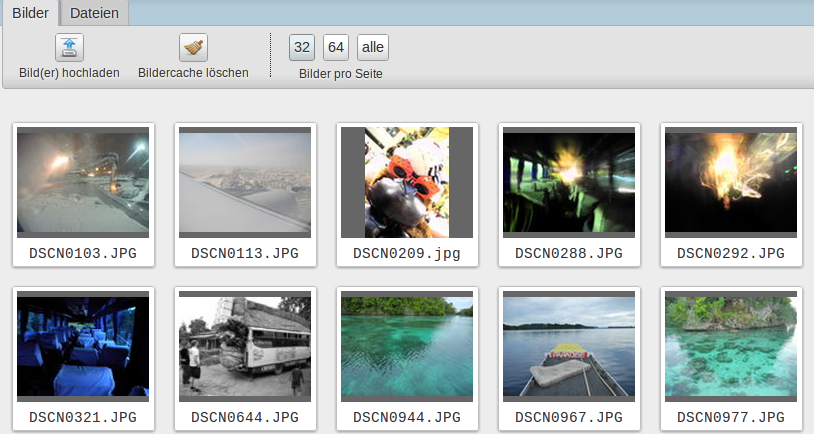
\includegraphics[scale=0.5]{images/analyse/alchemy/ressourcen.png}
\caption{Ressourcen-Auflistung ohne Möglichkeiten der Strukturierung in Alchemy CMS. Für die anderen Systeme ergibt sich ein ähnliches Gesamtbild.}
\end{center}
\end{figure}

\begin{lstlisting}[label=refineryoutput,caption=Beispiel für eine JavaScript-Funktion zur Realisierung des Bildauswahldialogs in Refinery CMS. Das Codebeispiel zeigt ebenfalls die Abhängigkeit zu dem verwendeten HTML-Markup (z.B. Zeile 18)]

var image_dialog = {
  initialised: false
  , callback: null
  , init: function(callback){
    if (!this.initialised) {
      this.callback = callback;
      this.init_tabs();
      this.init_select();
      this.init_actions();
      this.initialised = true;
    }
    return this;
  }
  //...
  , set_image: function(img){
    if ($(img).length > 0) {
      $('#existing_image_area_content ul li.selected').removeClass('selected');
      $(img).parent().addClass('selected');
      var imageId = $(img).attr('data-id');
      var geometry = $('#existing_image_size_area li.selected a').attr('data-geometry');
      var size = $('#existing_image_size_area li.selected a').attr('data-size');
      var resize = $("#wants_to_resize_image").is(':checked');
      image_url = resize ? $(img).attr('data-' + size) : $(img).attr('data-original');

      if (parent) {
        if ((wym_src = parent.document.getElementById('wym_src')) != null) {
          wym_src.value = image_url;
        }
        if ((wym_title = parent.document.getElementById('wym_title')) != null) {
          wym_title.value = $(img).attr('title');
        }
        if ((wym_alt = parent.document.getElementById('wym_alt')) != null) {
          wym_alt.value = $(img).attr('alt');
        }
        if ((wym_size = parent.document.getElementById('wym_size')) != null
            && typeof(geometry) != 'undefined') {
          wym_size.value = geometry.replace(/[<>=]/g, '');
        }
      }
    }
  }
  //...
};
\end{lstlisting}


\chapter{Lösungsvorschläge}
In diesem Kapitel werden Lösungsvorschläge zur Beseitigung der in Kapitel 4 beschriebenen Probleme formuliert.
\section{Implementierung eines Ruby on Rails Content Repository}

Die in den analysierten WCMS umgesetzten Implementierungen der Erweiterungsentwicklung verstoßen zum Teil gegen das in Rails gebotene Prinzip des DRY (vgl. Kapitel \ref{dryverstoss}). Eine konzeptionelle Änderung innerhalb dieses Systembereiches hätte somit Auswirkungen auf die gesamte WCMS-Infrastruktur der Inhaltsspeicherung. Dennoch soll hier der mögliche Lösungsansatz eines Content Repository konzeptionell vorgestellt werden.


\subsection{Idee und Konzept}

Heutige Webanwendungen (u.a. auch Web Content Management Systeme) benötigen neben der klassischen Speicherung von Daten zahlreiche zusätzliche Daten-Management-Funktionalitäten. Ein Content Repository (CR) soll dieser Entwicklung Rechnung tragen und definiert daher ein abstraktes Datenmodell zur Datenspeicherung und zusätzliche Servicefunktionalitäten, die häufig von content-orientierten Anwendungen verwendet werden. Ein Content Repository stellt somit u.a. folgendes Leistungsspektrum bereit:

\begin{itemize}
\item
Speicherung strukturierter und unstrukturierter Daten (z.B. Binär- und Textformate oder Metadaten),
\item
Möglichkeiten der Zugangskontrolle
\item
Möglichkeiten der Sperrung (Locking)
\item
Durchführung von Transaktionen
\item
Versionierungsmechanismen
\item
Überwachung von Daten
\item
Volltextsuche
\end{itemize}

Der Zugriff auf das Content Repository wird dabei durch eine API genau definiert und garantiert somit einen definierten Zugriff auf die zusäzlichen Funktionalitäten. Andere Entwickler können auf das Content Repository und seine Zusatzfunktionen kontrolliert zugreifen, ohne etwas über die Infrastruktur und seine Implementierungsdetails zu wissen. Intern greift das Content Repository auf andere Technologien und Infrastrukturen zurück, um die geforderten Funktionalitäten abzubilden\footnote{Das im folgenden beschriebene Java Content Repository Jackrabbit verwendet in seiner Standardkonfiguration z.B. WebDAV zur Speicherung von Daten sowie Apache Lucene zur Realsierung der Suchindexierung.}.

Im Bereich der Java Enterprise Content Management Systeme werden Content Repositories bereits erfolgreich eingesetzt. Namhafte Beispiele sind dabei das kommerzielle ECMS CQ5 und CRX\footnote{Nach der Übernahme von Day Inc. durch Adobe im Sommer 2010 wird das angebotene Content Management System CRX als Adobe Projekt weitervertrieben.} von Adobe und das u.a. als Open Source Software verfügbare Alfresco ECMS\footnote{Informationen zu Alfresco und dem Content Repository: \href{http://www.alfresco.com/products/platform/}{http://www.alfresco.com/products/platform/}}.
Innerhalb der PHP-Entwicklergemeinde wird ebenfalls gerade an der Umsetzung eines auf PHP basierten Content Repositories gearbeitet. Initiatoren sind dabei vor allem die Typo3 Association mit einer Implementierung innerhalb des neuen Web Content Management Systems Typo3 5.0\footnote{Das TYPO3CR ist als eigenständiges Paket im PHP-FLOW3-Framework verfügbar und ein zentraler Bestandteil von Typo3 5.0}.


\subsection{Das Java Content Repository (JCR)}

Unter der Leitung von David Nüscheler der Firma Day Software wurde 2005 die erste Version einer Implementierung und API Spezifikation eines Java Content Repository veröffentlicht\footnote{Die Entwicklung ging im Java Specification Request (JSR) 170 als offizieller Standard in die Programmiersprache Java ein. Momentan wird an der Veröffentlichung der Version 2.0 des Standards gearbeitet(JSR-283).}. Die umgesetzte Referenzimplementierung wurde später unter der Leitung der Apache Foundation als Open Source Projekt Jackrabbit\footnote{Projektseite: \href{http://jackrabbit.apache.org/}{http://jackrabbit.apache.org/}} der Öffentlichkeit zur Verfügung gestellt.

Zur Speicherung der Inhalte definiert das Java Content Repository ein einfaches hierarchisches Datemmodell, das folgende Objektstruktur aufweist:


\begin{figure}[!h]
\begin{center}
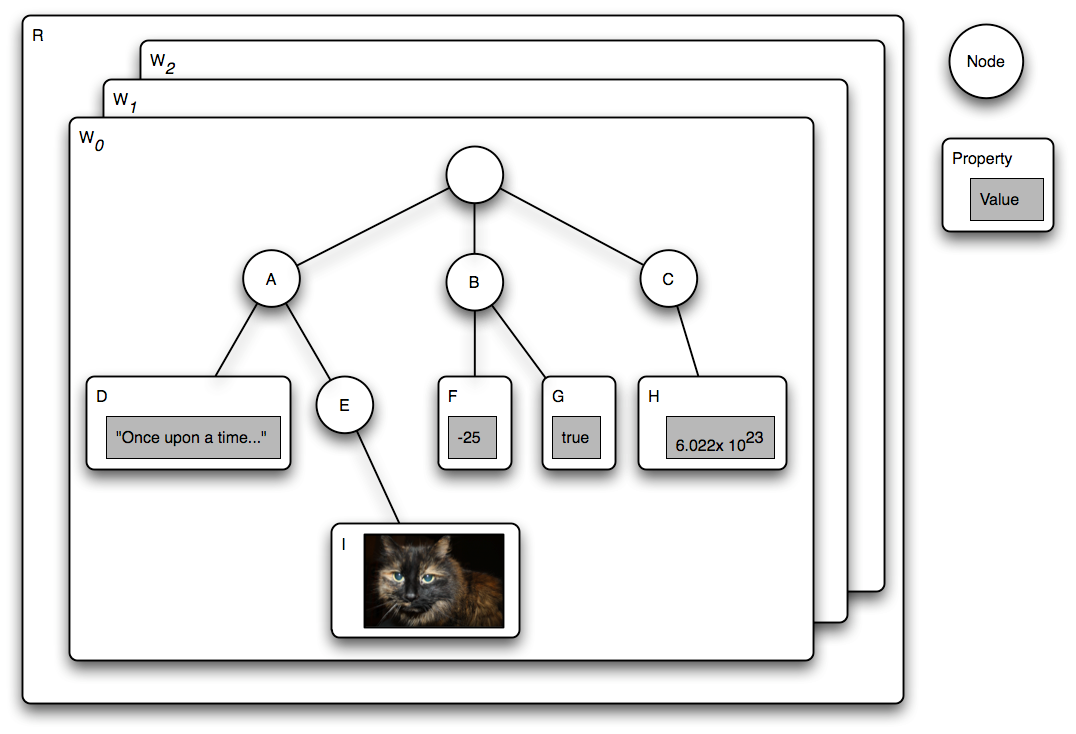
\includegraphics[scale=0.4]{images/repository/repository_diagramm.png}
\caption{JCR-Datenmodell}
\label{jcrdatenmodell}
\end{center}
\end{figure}



\begin{description}
\item[Workspace]\mbox{~}\\*
Ein JCR-Repository besteht aus einem oder mehreren Workspaces (Arbeitsbereichen), die jeweils mehrere Items in einer Baumstruktur beliebiger Tiefe verwalten können. Jeder Workspace lässt sich durch einen Namen eindeutig identifizieren (W\textsubscript{0}, W\textsubscript{1}, W\textsubscript{2}) und enthält mindestens ein Item (root node).
\item[Item]\mbox{~}\\*
Ein Item kann entweder ein Node (Knoten) oder ein Property (Eigenschaft) sein.
\item[Node]\mbox{~}\\*
Knoten (Nodes) eines Workspaces bilden die Struktur der zu speichernden Daten ab.
Ein Knoten kann daher keine oder weitere andere Kinderknoten (child notes) enthalten.
\item[Property]\mbox{~}\\*
Eine Property kann keine anderen Items beinhalten, aber dafür den Inhalt in Form von sogenannten Values abspeichern. Dabei kann ein Property-Node keine oder mehrere Values beinhalten.
\end{description}




\subsection{Umsetzungsvarianten innerhalb von Ruby on Rails}

Durch die Verfügbarkeit eines Ruby-Interpreter in der Programmiersprache Java (jruby\footnote{Projektseite: \href{http://jruby.org/}{http://jruby.org/}}) ergeben sich für die Umsetzung in Ruby on Rails folgende 2 Möglichkeiten:

\begin{itemize}
\item
Verwendung der Open Source Java Implementierung Jackrabbit und Spezifikation einer API zur Nutzung dieser innerhalb von Rails. Erste Implementierungsversuche und Demonstrationsanwendungen wurden bereits erstellt\footnote{Eine mit Rails 2 umgesetzte Demo-Anwendung ist unter folgender Internetseite verfügbar: \href{https://github.com/wpc/jcr-rails-demo}{https://github.com/wpc/jcr-rails-demo}. Sie zeigt dabei lediglich das Grundgerüst zur Umsetzung eines Content Repository auf.}.
\item
Erstellung einer eigenständigen, komplett auf Ruby und dem Rails Framework basierenden Referenzimplementierung und API nach dem Vorbild des Java Content Repository
\end{itemize}


\subsection{Vorteile für die gewählten Ruby on Rails WCMS}

Die Umsetzung eines Content Repository in Ruby kann für die bestehenden Web Content Management Systeme folgende Vorzüge bringen:

\begin{itemize}
\item Beseitigung des DRY-Verstosses bei den untersuchten Rails-WCMS, da die Inhalte in dem durch das Content Repository zur Verfügung gestellten hierarchischen Datenmodell gespeichert werden können.
\item
Wegfall der bisher notwendigen Datenbankmigrationen und zusätzlichen Datenbanktabellen, da das Content Repository die gesamte Infrastruktur bereitstellt und die Speicherung der Daten übernimmt.
\item Vereinfachung des Zugriffs auf Inhalte innerhalb verschiedener Systeme durch Verwendung einer definierten API
\item Fehlende Webpublishing-Funktionalitäten der existierenden Rails WCMS können durch eine Implementierung eines Content Repository als Infrastruktur allgemein zur Verfügung gestellt werden (z.B. Versionierung, Suchfunktionen).
\item Durch die im JCR-Standard festgelegten Import- und Exportfunktionen kann ein Austausch der Inhalte zwischen verschiedenen Web Content Management Systemen ermöglicht werden.
\item Ein Content Repository kann als Erweiterung auch von anderen Rails-Anwendungen verwendet werden, die mit verschiedenartig strukturierten Inhalten umgehen müssen.
\end{itemize}



\section{Übertragung des Typo3 5.0 Phoenix User-Interfaces in Rails 3.1}
Content Management Systeme erfordern bei steigender Funktionalität ein entsprechend komplexeres Nutzer-Interface. Die sinnvolle Realisierung entsprechender Oberflächen ist mit der u.a. in Refinery CMS gewählten Generierung von HTML-Views und einzelnen JavaScript-Dateien nur noch schwer möglich. Zur Umsetzung solcher Projekte empfiehlt sich daher der Einsatz alternativer Technologien.
Die neue Version 5.0 des PHP basierten Web Content Management Systems Typo3 greift bei der Generierung der gesamten Backend-Oberfläche auf das Java Script Frameworks Ext JS 4\footnote{Informationen und Download: \href{http://www.sencha.com/}{http://www.sencha.com/}} zurück. Es ermöglicht durch Kombinierung vorgefertigter Elemente eine schnelle Erstellung komplexer Oberflächen\footnote{Beispielanwendungen: \href{http://dev.sencha.com/deploy/ext-4.0.0/examples/}{http://dev.sencha.com/deploy/ext-4.0.0/examples/}}.
Die Veröffentlichung des Typo3-Projektes unter der GPLv3-Lizenz macht eine Weiternutzung der in der Version 5.0 geplanten Oberfläche generell möglich. Im folgenden sollen daher die notwendigen Schritte zur Integrierung des Typo3 5.0 User-Interfaces in eine Rails 3.1 Anwendung beschrieben werden.

\subsection{Typo3 5.0}
Die Entwicklung von Typo3 5.0 befindet sich noch in einer frühen Phase. Interessenten können jedoch bereits Entwicklerversionen in Form sogenannter Sprint Releases herunterladen und testen. Neben einem Download-Paket\footnote{Komponenten-Download: \href{http://flow3.typo3.org/typo3-phoenix/}{http://flow3.typo3.org/typo3-phoenix/}} auf der Projektseite von Typo3 wird zusätzlich eine aktuelle Version von Typo3 als Live-Demo\footnote{Demoseite: \href{http://phoenix.demo.typo3.org/}{http://phoenix.demo.typo3.org/}} angeboten. Die Zugangsdaten zum Backend können im Frontend der Seite mit Hilfe eines Formulars erzeugt werden.


\begin{figure}[!h]
\begin{center}
\label{fig.typo3frontend}
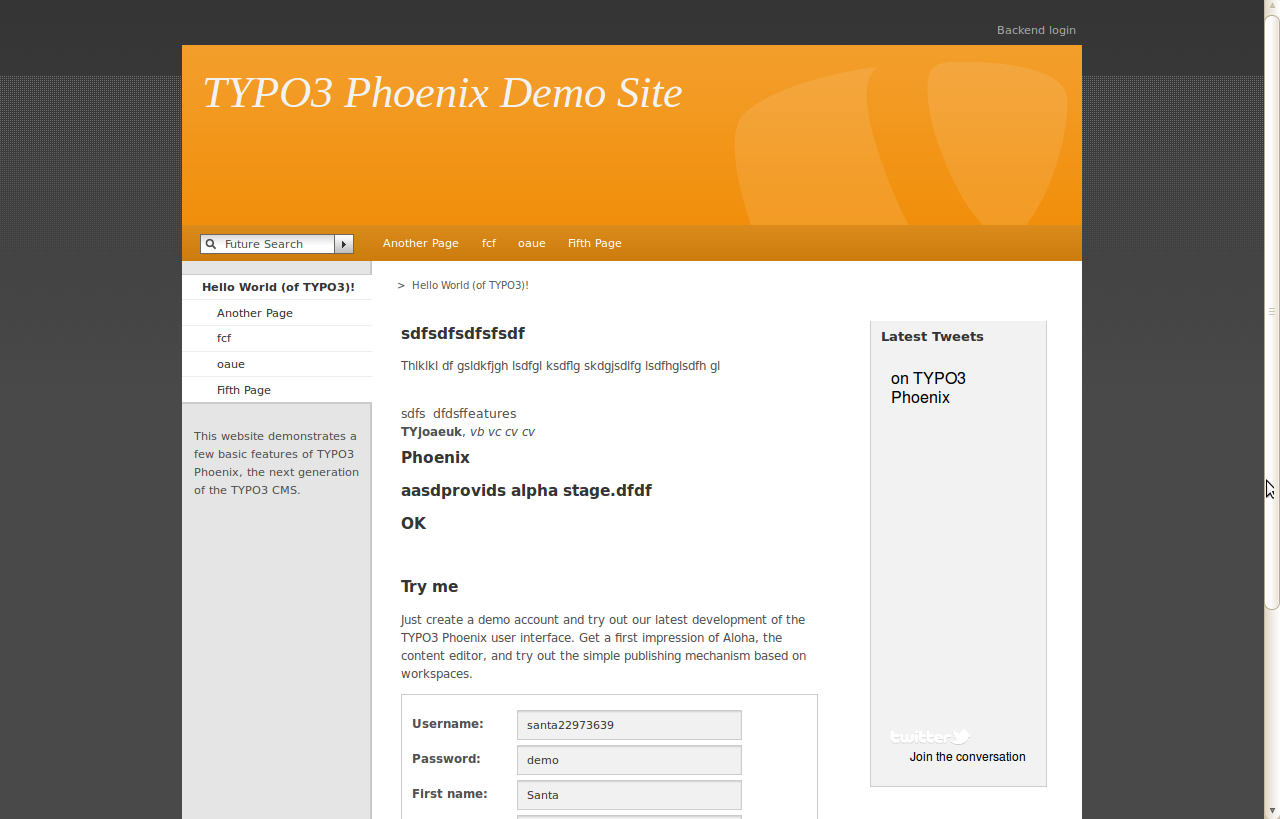
\includegraphics[scale=0.35]{images/typo3/frontend.png}
\caption{Frontend-Ansicht der Typo3 5.0 Sprint Release 6 Demoversion}
\end{center}
\end{figure}


\begin{figure}[!h]
\begin{center}
\label{fig.typo3backend}
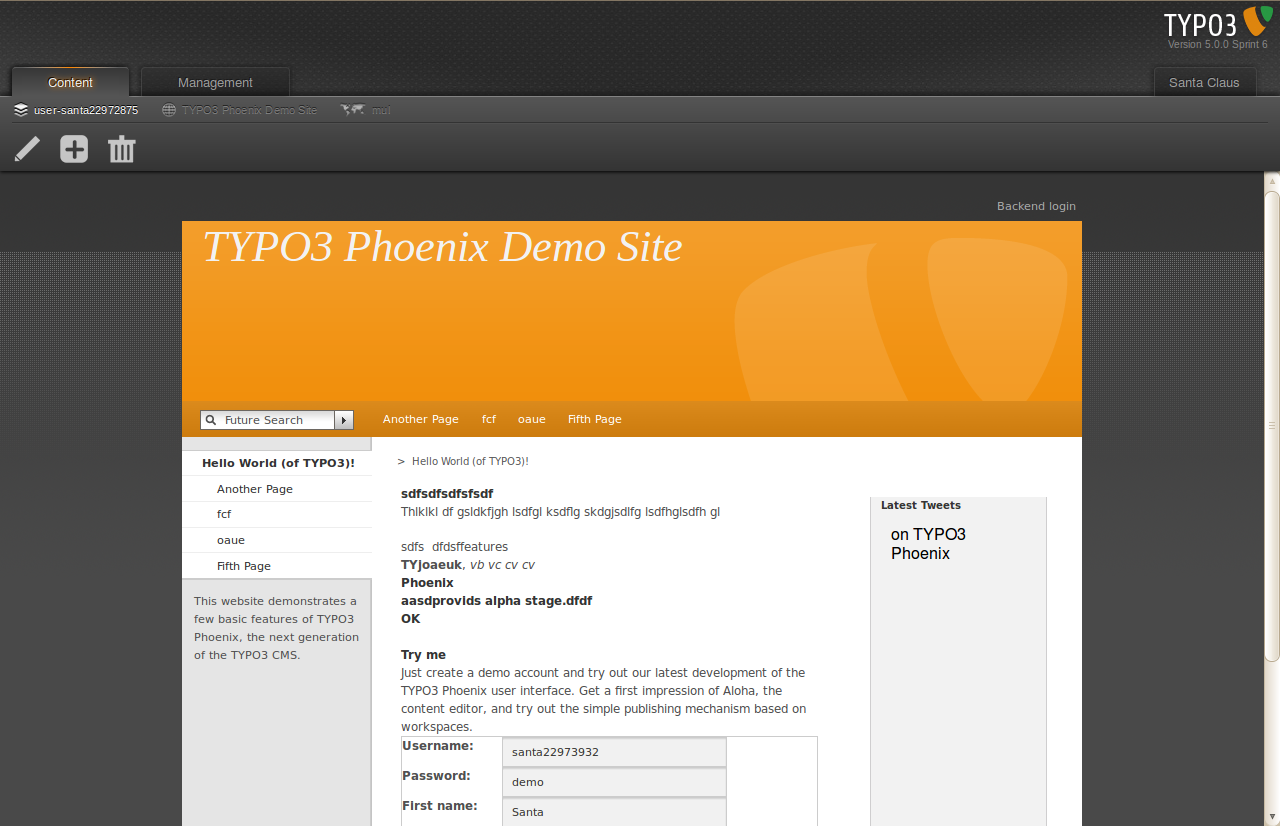
\includegraphics[scale=0.35]{images/typo3/backend.png}
\caption{Backend-Ansicht der Typo3 5.0 Sprint Release 6 Demoversion}
\end{center}
\end{figure}
\newpage
Das in der Demoversion umgesetzte Nutzer-Interface repräsentiert nur einen Teil der für Typo3 5.0 geplanten Oberfläche und Komponenten\footnote{Bilder und ausführliche Erläuterungen zur neuen Typo3 5.0 Oberfläche sind unter folgender Adresse zu finden: \href{http://typo3.org/teams/usability/t35ui/}{http://typo3.org/teams/usability/t35ui/}}. U.a. sind folgende Bestandteile bereits umgesetzt wurden:
\begin{itemize}
\item
Login-Seite zur Anmeldung im Backend von Typo3 5.0
\item
Content-Modul im Backend mit integrierter Vorschau der aktuell ausgewählten Seite und beschränkten Möglichkeiten der Inhaltsbearbeitung mit Hilfe des für Typo3 5.0 geplanten Aloha-Editors
\item
Management-Modul zur Verwaltung der im System angelegten Seiten in Form einer Baumstruktur
\item
Dashboard des angemeldeten Nutzers mit Auflistung der editierten Inhalte
\end{itemize}


\subsection{Ext JS und Ext Direct}

Das Typo3-User-Interface setzt bei der Kommunikation zwischen den einzelnen Interface-Komponenten und dem Server auf die Nutzung von Ext Direct. Ext Direct beschreibt dabei einen in Ext JS definierten Sprachstandard, mit dessen Hilfe serverseitige Funktionen clientseitig per JavaScript aufgerufen werden können.
Für ein besseres Verständnis wird in Abbildung \ref{extinvoke} eine im jQuery Framework formulierte Ajax-Anfrage und der entsprechende Ext Direct Ausdruck gegenübergestellt.

\begin{lstlisting}[label=extinvoke, caption=Ajax-Anfrage an einen Server im jQuery-Framework]

// jQuery Ajax Request
$.ajax({
  url: '/ajax?ajaxID=MyController_myMethod&amp;parameter1=someValue',
   success: function( data ) {
    alert(data);
    }
  }
});

// Ext Direct Aufruf
Namespace.MyController.myMethod("some_Value", function(data, e) {
  	alert(data);
});

\end{lstlisting}

Beide JavaScript-Beispiele resultieren in einer asynchronen Ajax-Anfrage, die die entsprechende Methode serverseitig aufruft. Für Ext Direct ergeben sich jedoch folgende zusätzliche Vorteile:

\begin{enumerate}
\item
Keine wiederholte Angabe einer URL zum Aufruf der serverseitigen Funktionen.
\item
Vereinfachung des JavaScript-Quellcodes, da im Vergleich zu herkömmlichen asynchronen Anfragen weniger Quellcode geschrieben werden muss.
\item
Vereinfachung der cleintseitigen JavaScript-Programmierung, da der Aufruf von client- und serverseitigen Methoden namentlich übereinstimmt.
\end{enumerate}

Eine umfassende Beschreibung von Ext Direct ist dem Anhang der Arbeit beigefügt (Anhang \ref{extspec}). Dort werden alle Konzepte und notwendigen Komponenten für eine serverseitige Unterstützung von Ext Direct erläutert.


Um Ext Direct auch innerhalb einer Rails-Anwendung nutzbar zu machen, wurde im Rahmen dieser Diplomarbeit die Rails 3.1 kompatible Erweiterung \emph{extr} entwickelt\footnote{Für Ruby und das Rails-Framework existieren bereits Implementierungen, die jedoch nicht vollständig zu Rails 3 und 3.1 kompatibel sind. Aus diesem Grund wurde die Umsetzung einer eigenen Erweiterung ins Auge gefasst.}.
Der für Ext Direct notwendige Router (Anhang \ref{extspec}) wurde dabei mit Hilfe einer Rack Middleware realisiert, die alle Ext JS-Anfragen an die entsprechenden Serverseitigen Methoden (Controller-Methoden) weiterleitet. Schematisch ergibt sich somit folgender Anfrageablauf innerhalb der Rails-Anwendung:

\begin{figure}[!ht]
\begin{center}
\label{fig.directrouter}
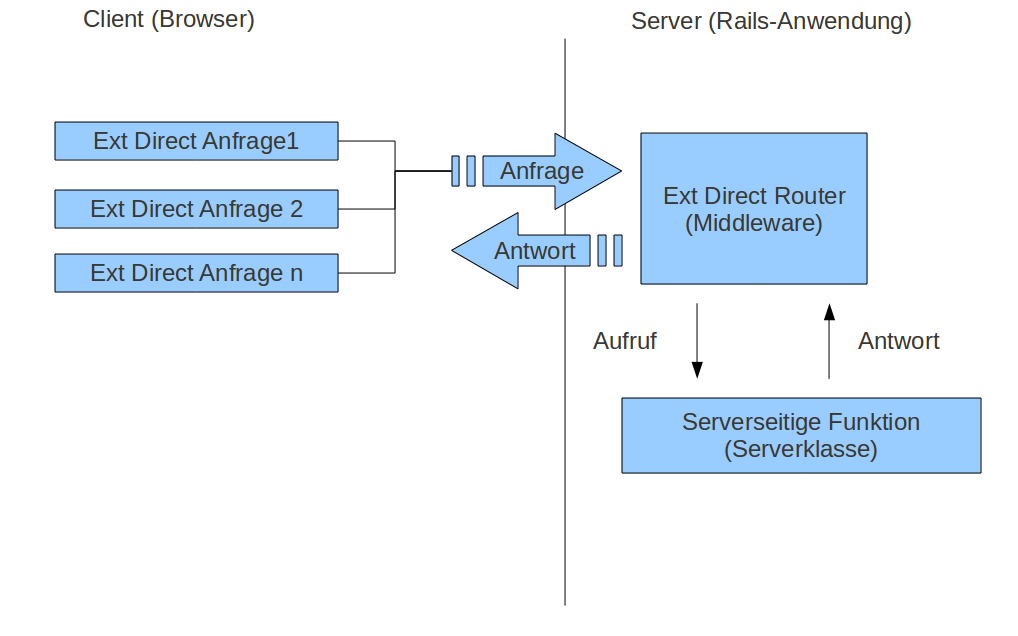
\includegraphics[scale=0.55]{images/rack/extdirect.png}
\caption{Schema des Ext Direct Routing mit \emph{extr}}
\end{center}
\end{figure}

Die Installation und Nutzung der Erweiterung \emph{extr} wird im Anhang dieser Arbeit demonstriert. Auf Grund des frühen Entwicklungsstatus unterstützt die Erweiterung serverseitig noch nicht alle der geforderten Ext-Direct-Funktionalitäten. Im folgenden sollen bestehende Beschränkungen und Probleme erläutert werden:
\begin{itemize}
\item
Ext Direct-Anfragen mit Parametern aus Formularen und Datei-Uploads (Form Posts) werden von der Rails Middleware noch nicht vollständig an die entsprechende Zielmethode (controller action) weitergeleitet.
\item
kein Schutz vor CSRF/XSRF-Angriffen\footnote{Cross Site Request Forgery beschreibt einen Angriff auf eine Webanwendung durch Aufruf einer manipulierenden Aktion über eine beliebige andere Internetseite. Nähere Erläuterungen unter folgender Adresse: \href{http://guides.rubyonrails.org/security.html\#cross-site-request-forgery-csrf}{http://guides.rubyonrails.org/security.html\#cross-site-request-forgery-csrf}}
\end{itemize}

\subsection{Umgesetzte Rails-Anwendung}
Durch die Realisierung der Erweiterung \emph{extr} kann eine Übertragung des Typo3-UI in Rails 3.1 möglich gemacht werden. Die dabei vom Typo3-Projekt benötigten JavaScript-Dateien wurden dafür unverändert in eine neu erzeugte Rails 3.1-Anwendung integriert und als Backend-Bereich in der Rails-Anwendung zum Aufruf über den Browser freigeschalten. Die erzeugte Anwendung steht dabei als Download-Paket und Online-Version zur Verfügung:
\begin{table}[!h]
\begin{tabular}{|l|p{10cm}|}
\hline
Download Quellcode & https://github.com/skeller1/phoenixR \\
\hline
Online-Version & http://phoenix.herokuapp.com/ \\
\hline
Nutzername & demo \\
\hline
Passwort & demo \\
\hline
\end{tabular}
\end{table}

\subsection{Vorteile der Typo3-Nutzeroberfläche}
Die Nutzung der Typo3-Nutzeroberfläche (und EXT JS) ergibt folgende Vorteile für Anwender und Entwickler:
\begin{itemize}
\item
Ein Modularer Aufbau der Nutzoberfläche mit Möglichkeiten der Überschreibung und Erweiterung bestehender Komponenten der Nutzeroberfläche ist möglich.
\item
Die Verfügbarkeit erprobter, flexibler und vielfach genutzter UI-Komponenten (z.B. variable Listen, Dialoge, Baumstrukturen u.a.) ermöglicht die Realisierung einer konsistenten Nutzeroberfläche.
\item
Das Backend (Backend-View, Bilder, CSS und JavaScript) wird einmalig vom Server ausgeliefert und steht danach zur Nutzung im Browser zur Verfügung. Nur bei Bedarf werden Anfragen an den Server gestartet, um neue Daten für Nutzerinteraktionen bereit zustellen.
\item
EXT JS garantiert eine größtmögliche Kompatibilität zu aktuellen Internet-Browsern (Internet Explorer, Firefox, Safari, Chrome u.a)
\end{itemize}


\chapter{Zusammenfassung}

\section{Fazit}

Im Rahmen dieser Arbeit konnten die ausgewählten Ruby on Rails Web Content Management Systeme Alchemy CMS, Browser CMS, Locomotive CMS und Refinery CMS auf ihre Webpublishing-Fähigkeiten untersucht werden. Dabei zeigte sich, dass der allgemein in Content Management Systemen etablierte Redaktionsprozess (Erstellung, Verwaltung, Publikation und Archivierung) sehr unterschiedlich unterstützt wird.
Ein Einsatz der Systeme kann daher nur empfohlen werden, wenn in einer Voranalyse die Anforderungen an die tatsächlich umzusetzende Internetseite genau definiert und mit dem gewünschten Rails WCMS abgeglichen werden. Zwar bietet Rails komfortable Möglichkeiten zur Anpassung der Systeme, dies erfordert jedoch einen erhöhten Mehraufwand im Vergleich zu verbreiteten Lösungen wie Typo3 oder Drupal, die im Bereich des Webpublishing bereits einen Großteil der hier untersuchten Funktionalitäten erfüllen.
Die in Kapitel \ref{chap:probleme} aufgezeigten Implementierungsdetails zeigen darüber hinaus, das die Systeme hinsichtlich ihres Datenbankdesigns und der User-Interface-Umsetzung Optimierungspotenzial besitzen. Vor allem der in Rails übliche Einsatz von Generatorskripten und HTML-Views bei der Erweiterungsentwicklung lässt die Arbeit mit diesen Systemen schnell unübersichtlich und aufwendig erscheinen.

\section{Ausblick}
Die vorgestellten WCMS sind zum Teil erst innerhalb der letzten 2 Jahre (2009) an die Öffentlichkeit übergeben wurden. Durch die Leistungen der Open Source-Bewegung ist daher mit weiteren funktionalen und technischen Verbesserungen zu rechnen. Die Umsetzung eines rails-basierten Content Repository kann dabei einen wichtigen Entwicklungsimpuls innerhalb der Ruby on Rails Web Content Management Systeme bedeuten.


\chapter{Anhang}
\section{Liste bestehender Open Source Rails 2 und 3 Web Content Management Systeme bzw. Blogging-Software}

\begin{table}[!ht]
\center
\begin{tabular}[]{|p{3cm}|p{8cm}|p{4cm}|}
% Begin Rails 2
\hline
\multicolumn{3}{|p{15cm}|}{\textbf{OpenSource Web Content Management Systeme mit Rails 2.x Unterstützung}}\\
\hline
\textbf{Projektname}&\textbf{Projektseite im Internet}&\textbf{Aktive Weiterentwicklung}\\
\hline
adva-cms & \href{https://github.com/svenfuchs/adva\_cms}{https://github.com/svenfuchs/adva\_cms} & Ja \\
\hline
\cellcolor{alicegrey} Alchemy CMS & \cellcolor{alicegrey} \href{http://magiclabs.github.com/alchemy/}{http://magiclabs.github.com/alchemy/} & \cellcolor{alicegrey} Ja \\
\hline
Ansuz CMS & \href{https://github.com/knewter/ansuz}{https://github.com/knewter/ansuz} & eingestellt\\
\hline
Casein & \href{http://www.caseincms.com/}{http://www.caseincms.com/} & Ja \\
\hline
Comatose & \href{http://comatose.rubyforge.org/}{http://comatose.rubyforge.org/} & eingestellt\\
\hline
Compages & \href{http://compages.wordpress.com/}{http://compages.wordpress.com/} & eingestellt\\
\hline
Geego CMS & \href{http://gitorious.org/geego-cms\#more}{http://gitorious.org/geego-cms\#more} & eingestellt\\
\hline
Skyline CMS & \href{http://www.skylinecms.nl/}{http://www.skylinecms.nl/} & Ja \\
\hline
Webiva & \href{http://webiva.org/}{http://webiva.org/} & Ja \\
\hline
Railfrog & \href{http://railfrog.com/}{http://railfrog.com/} & Nein \\
\hline
Radiant & \href{http://radiantcms.org/}{http://radiantcms.org/} & Ja \\
\hline
zenacms & \href{http://zenadmin.org/}{http://zenadmin.org/} & Ja \\
\hline
Mephisto & \href{https://github.com/halorgium/mephisto}{https://github.com/halorgium/mephisto} & eingestellt\\
\hline
Rubricks & \href{http://rubricks.org/}{http://rubricks.org/} & eingestellt\\
\hline
Typhus & \href{http://typus.heroku.com/}{http://typus.heroku.com/} & eingestellt\\
\hline
Station & \href{https://github.com/atd/station}{https://github.com/atd/station} & Ja\\
\hline
Vrame & \href{https://github.com/9elements/vrame}{https://github.com/9elements/vrame} & eingestellt\\
\hline
Rojo CMS & \href{https://github.com/onomojo/rojo}{https://github.com/onomojo/rojo} & unbekannt\\
\hline


\end{tabular}
\end{table}

% End Rails 2

% Begin Rails 3
\begin{table}
\center
\addtocounter{footnote}{1}
\begin{tabular}[]{|p{3cm}|p{8cm}|p{4cm}|}
\hline
\multicolumn{3}{|p{15cm}|}{\textbf{Open Source Web Content Management Systeme mit Rails 3.x Unterstützung}}\\
\hline
\textbf{Projektname}&\textbf{Projektseite im Internet}&\textbf{Aktive Weiterentwicklung}\\
\hline
\cellcolor{alicegrey}Alchemy CMS & \cellcolor{alicegrey} \href{http://magiclabs.github.com/alchemy/}{http://magiclabs.github.com/alchemy/} &\cellcolor{alicegrey} Ja \\
\hline
\cellcolor{alicegrey}Browser CMS & \cellcolor{alicegrey} \href{http://browsercms.org}{http://browsercms.org} & \cellcolor{alicegrey} Ja \\
\hline
Casein & \href{https://github.com/spoiledmilk/casein3}{https://github.com/spoiledmilk/casein3} & Ja \\
\hline
\cellcolor{alicegrey} Locomotive CMS & \cellcolor{alicegrey} \href{http://www.locomotivecms.com/}{http://www.locomotivecms.com/} & \cellcolor{alicegrey} Ja \\
\hline
\cellcolor{alicegrey} Refinery CMS & \cellcolor{alicegrey} \href{http://refinerycms.com/}{http://refinerycms.com/} & \cellcolor{alicegrey} Ja \\
\hline
adva-cms2 & \href{https://github.com/svenfuchs/adva-cms2}{https://github.com/svenfuchs/adva-cms2} & Ja \\
\hline
typo (Blogging) & \href{http://fdv.github.com/typo/}{http://fdv.github.com/typo/} & Ja \\
\hline
Surtout CMS & \href{http://surtoutcms.com/}{http://surtoutcms.com/} & noch nicht veröffentlicht \\
\hline
Nesta CMS & \href{https://github.com/gma/nesta}{https://github.com/gma/nesta} & ja  \\
\hline
Comfortable Mexican Sofa & \href{https://github.com/twg/comfortable-mexican-sofa}{https://github.com/twg/comfortable-mexican-sofa} & ja  \\
\hline
% End Rails 3
\end{tabular}
\end{table}

\begin{comment}
% begin closed source
\begin{table}
\center
\begin{tabular}[]{|p{3cm}|p{8cm}|p{4cm}|}
\hline
\multicolumn{3}{|p{15cm}|}{\textbf{Closed Source Web Content Management Systeme mit Rails 3.x Unterstützung}}\\
\hline
\textbf{Projektname}&\textbf{Projektseite im Internet}&\textbf{Aktive Weiterentwicklung}\\
\hline
Blocks & \href{http://www.blocksglobal.com/}{http://www.blocksglobal.com/} & Ja \\
\hline
% End clsoed source
\end{tabular}
\end{table}
\end{comment}

\pagebreak


\section{Crudify-Methode von Refinery CMS 1.0.8}


\lstinputlisting[label=crudify, nolol=true, title=Implementierung der Crudify-Methode in Refinery CMS 1.0.8,language=Ruby]{code/crudify_method.rb}

\section{Ext-Direct Spezifikation für Ext Js 3.0}
\label{extspec}
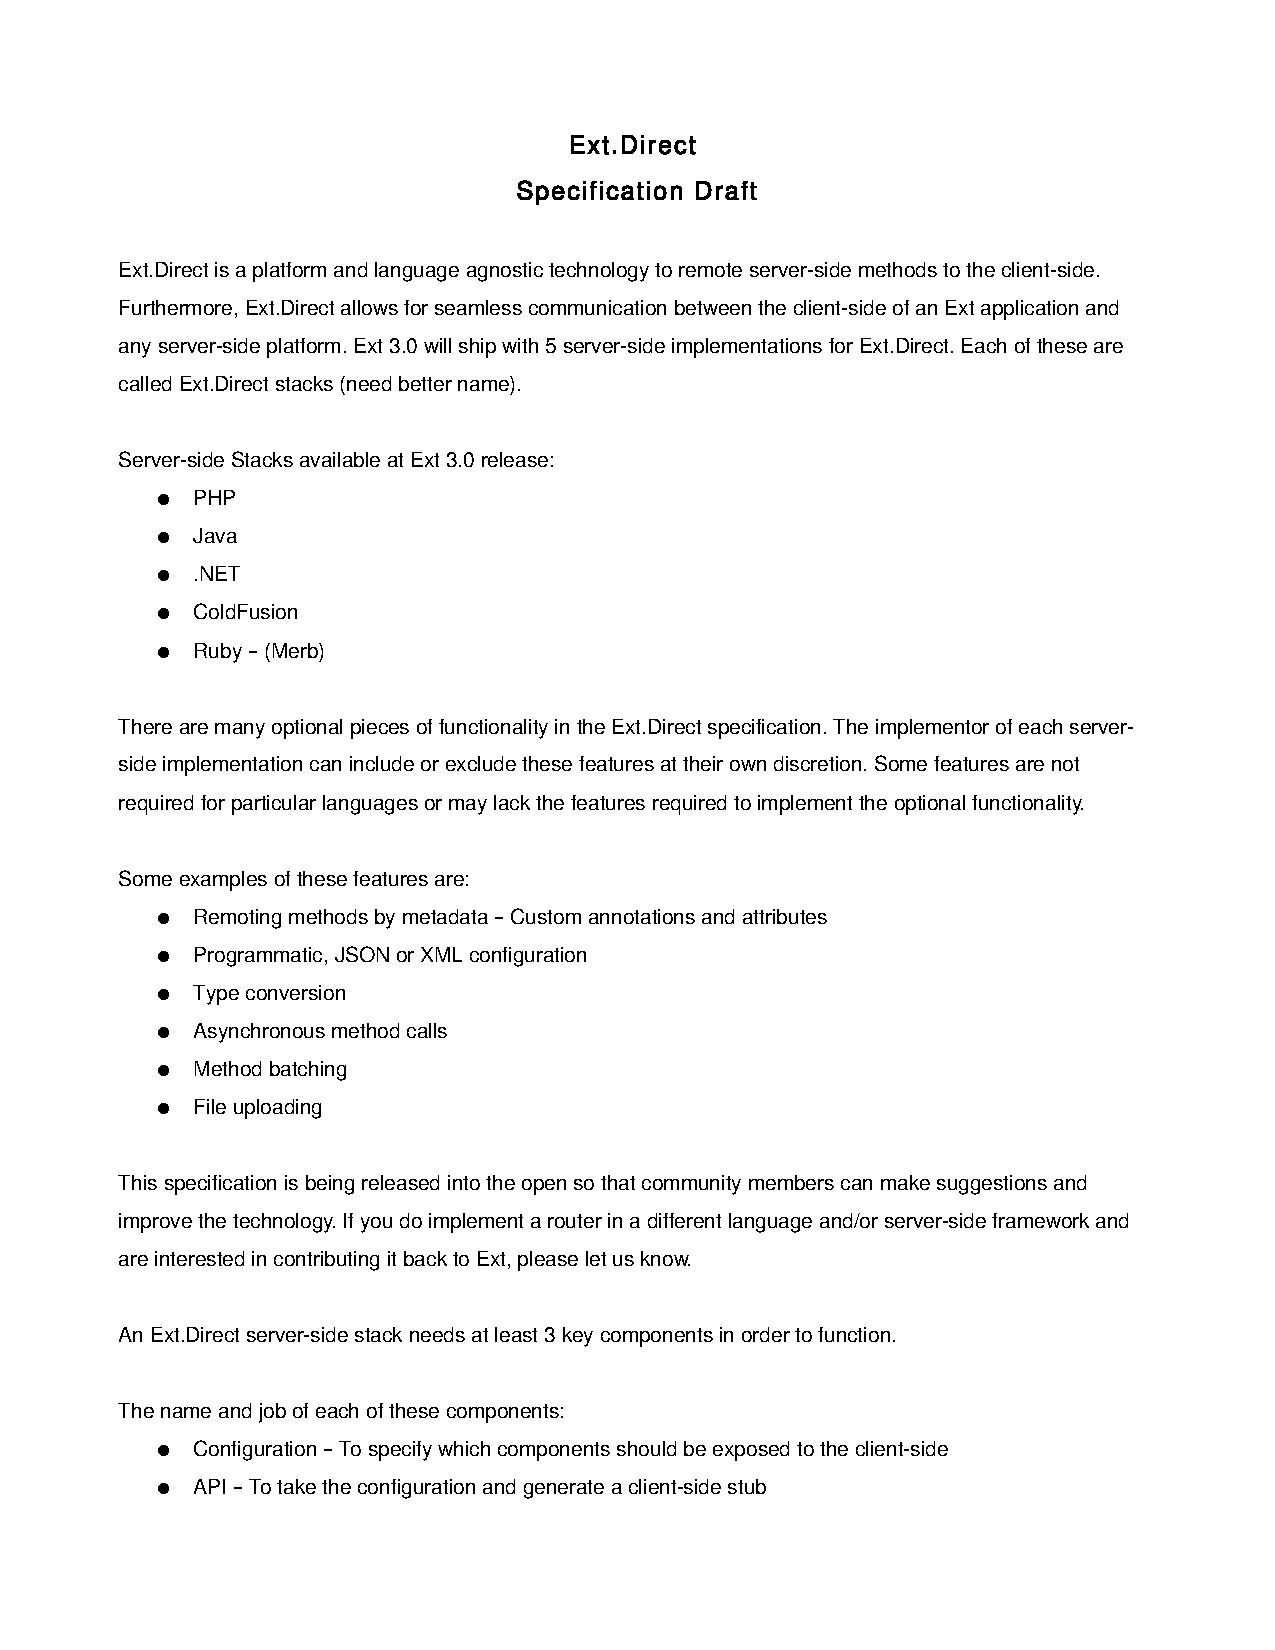
\includepdf{pdf/extdirect.pdf}

\section{Nutzung von Extr in einer Rails 3.1-Anwendung}


Im folgenden Abschnitt wird die Installation und Nutzung des erstellten Plugins Extr in einer neu erstellten Rails 3-Anwendung demonstriert. Das erstellte Paket ist noch in der Entwicklungsphase und konnte nicht vollständig auf seine Sicherheit überprüft werden\footnote{Sicherheitsbedenken in den Bereichen CSRF und XSS wurden bei der Vorstellung des Paktes aufgezeigt.}. Der Quellcode der Anwendung kann unter folgender Adresse heruntergeladen werden:

Extr: \href{https://github.com/skeller1/extr}{https://github.com/skeller1/extr}

Für die folgenden Beschreibungen wird eine funktionsbereite Rails 3.1-Installation vorausgesetzt.

\begin{enumerate}
\item
Erstellung einer neuen Rails 3-Anwendung \emph{directtest}
\begin{lstlisting}[frame=single, numbers=none]
rails new directtest
\end{lstlisting}
\item
Aktivierung des Plugins/Gems in der Gemfile der erstellten Rails-Anwendung

\begin{lstlisting}[frame=single, numbers=none]

# ...
gem "extr", :git => "git://github.com/skeller1/extr.git"
# ...

\end{lstlisting}

\item
Erstellung einer Rails 3 Standard-Ressource Projekt und Erzeugung der notwendigen Datenbanktabelle.

\begin{lstlisting}[frame=single, numbers=none]
rails g scaffold project name:string description:text
rake db:migrate
\end{lstlisting}

\item
Einbinden der notwendigen Ext-Direct-Bibliotheken mit Hilfe der vom Plugin zur Verfügung gestellten Helfermethoden (View Helpers). Der Namensraum des Ext-Direct-Provider ist \emph{Rails}.

\begin{lstlisting}[language=xml,frame=single,title=\emph{app/views/layouts/application.html.erb}, numbers=none]
<!DOCTYPE html>
<html>
<head>
  <title>Extr</title>
  <%= stylesheet_link_tag "extr/application" %>
  <%= javascript_include_tag "extr/application" %>
  <%= csrf_meta_tags %>
  <%= ext_base_tag %>
  <%= ext %>
  <%= ext_direct_provider "Rails" %>
</head>
<body>
    <%= yield %>
</body>
</html>
\end{lstlisting}

\item
Registrierung der Ext-Direct-fähigen Controller-Methoden (Actions) im Projekte-Controller (projects controller). Die erstellten Methoden sind nur als Beispiel zu verstehen und können entsprechend angepasst werden.

\begin{lstlisting}[language=ruby,frame=single,title=\emph{app/controllers/projects\_controller.rb}, numbers=none]
class ProjectsController < ApplicationController

  # activate extr for this controller
  include Extr::DirectController


  #disable Rails 3 authenticity_token for demonstration, not recom. in production
  skip_before_filter :verify_authenticity_token


  #register 2 ext direct controller action with different, optional controller name (MyDirectController)
  direct "MyDirectController",
    :getChildProject => 1,
    :someOtherMethod => 2


  def getChildProject
    # render a random project name as json response
    render :json => {:name => "Project#{Random.rand(11)}"}.to_json
  end

\end{lstlisting}

\item
Im Index-HTML-View der Projekt-Ressource (http://localhost:3000/projects) kann nun durch einen Javascript-Aufruf eine Anfrage an die registrierten Ext-Direct-Controller-Methoden gesendet werden. Abbildung \ref{extrreqeust} zeigt das Ergebnis eines mit Hilfe des Mozilla Firefox Plugins Firebug temporär ausgeführten JavaScript-Codes.
Als Javascript-Callback wird der Name des Projektes zurückgegeben (\emph{Project9}).
\begin{lstlisting}[language=ruby,frame=single,title=\emph{Javascript zum Aufruf des Projekt-Controllers in der Rails-Anwendung}]
Rails.MyDirectController.getChildProject("param",function(r,e){
 alert(r.name);
});

\end{lstlisting}

\begin{figure}[!h]
\begin{center}
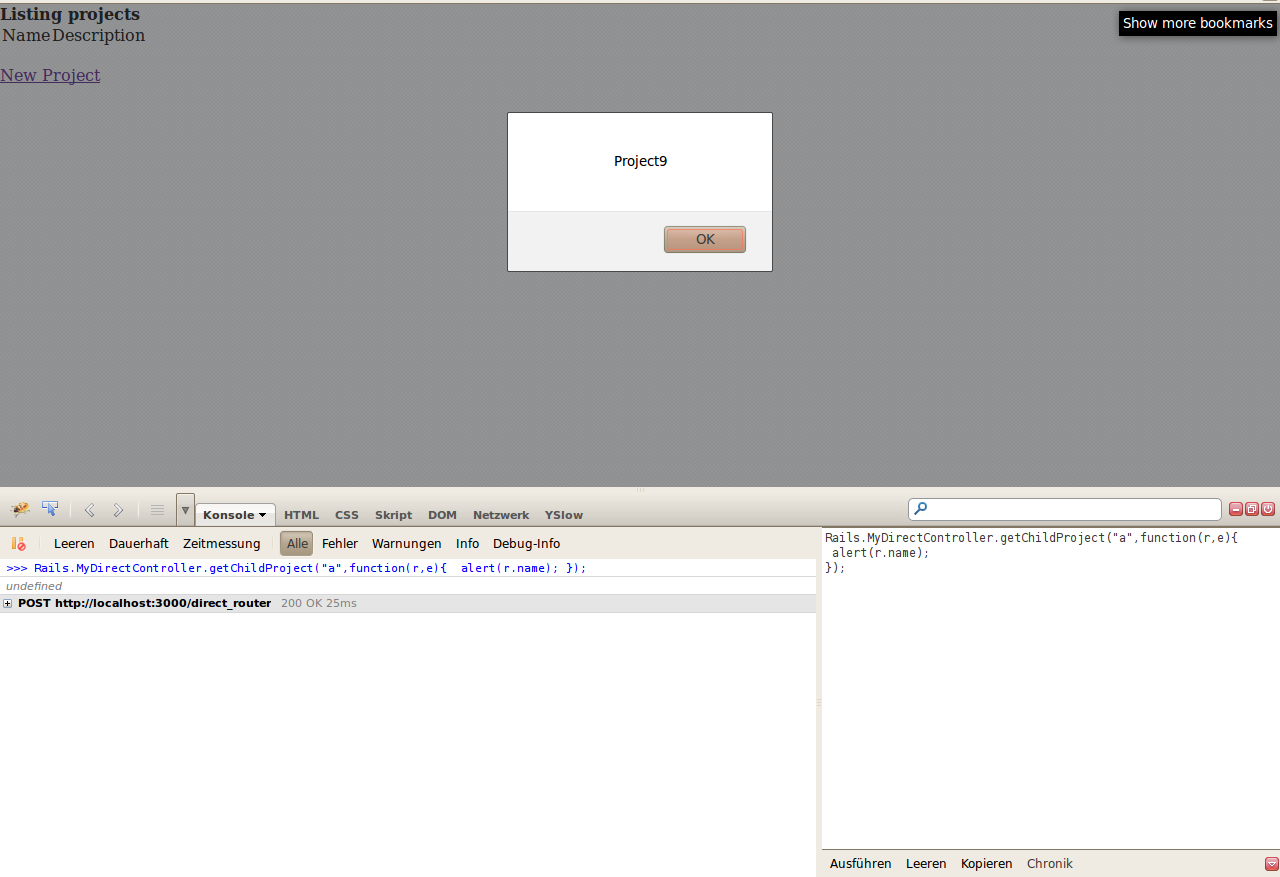
\includegraphics[scale=0.3]{images/anhang/extrbrowserrequest.png}
\caption{Mit Hilfe von Firebug formulierte Javascript-Ext-Direct-Anfrage mit ausgegebener Antwort der Rails-Anwendung}
\label{extrreqeust}
\end{center}
\end{figure}
\end{enumerate}

\section{Java Content Repository Spezifikation}
%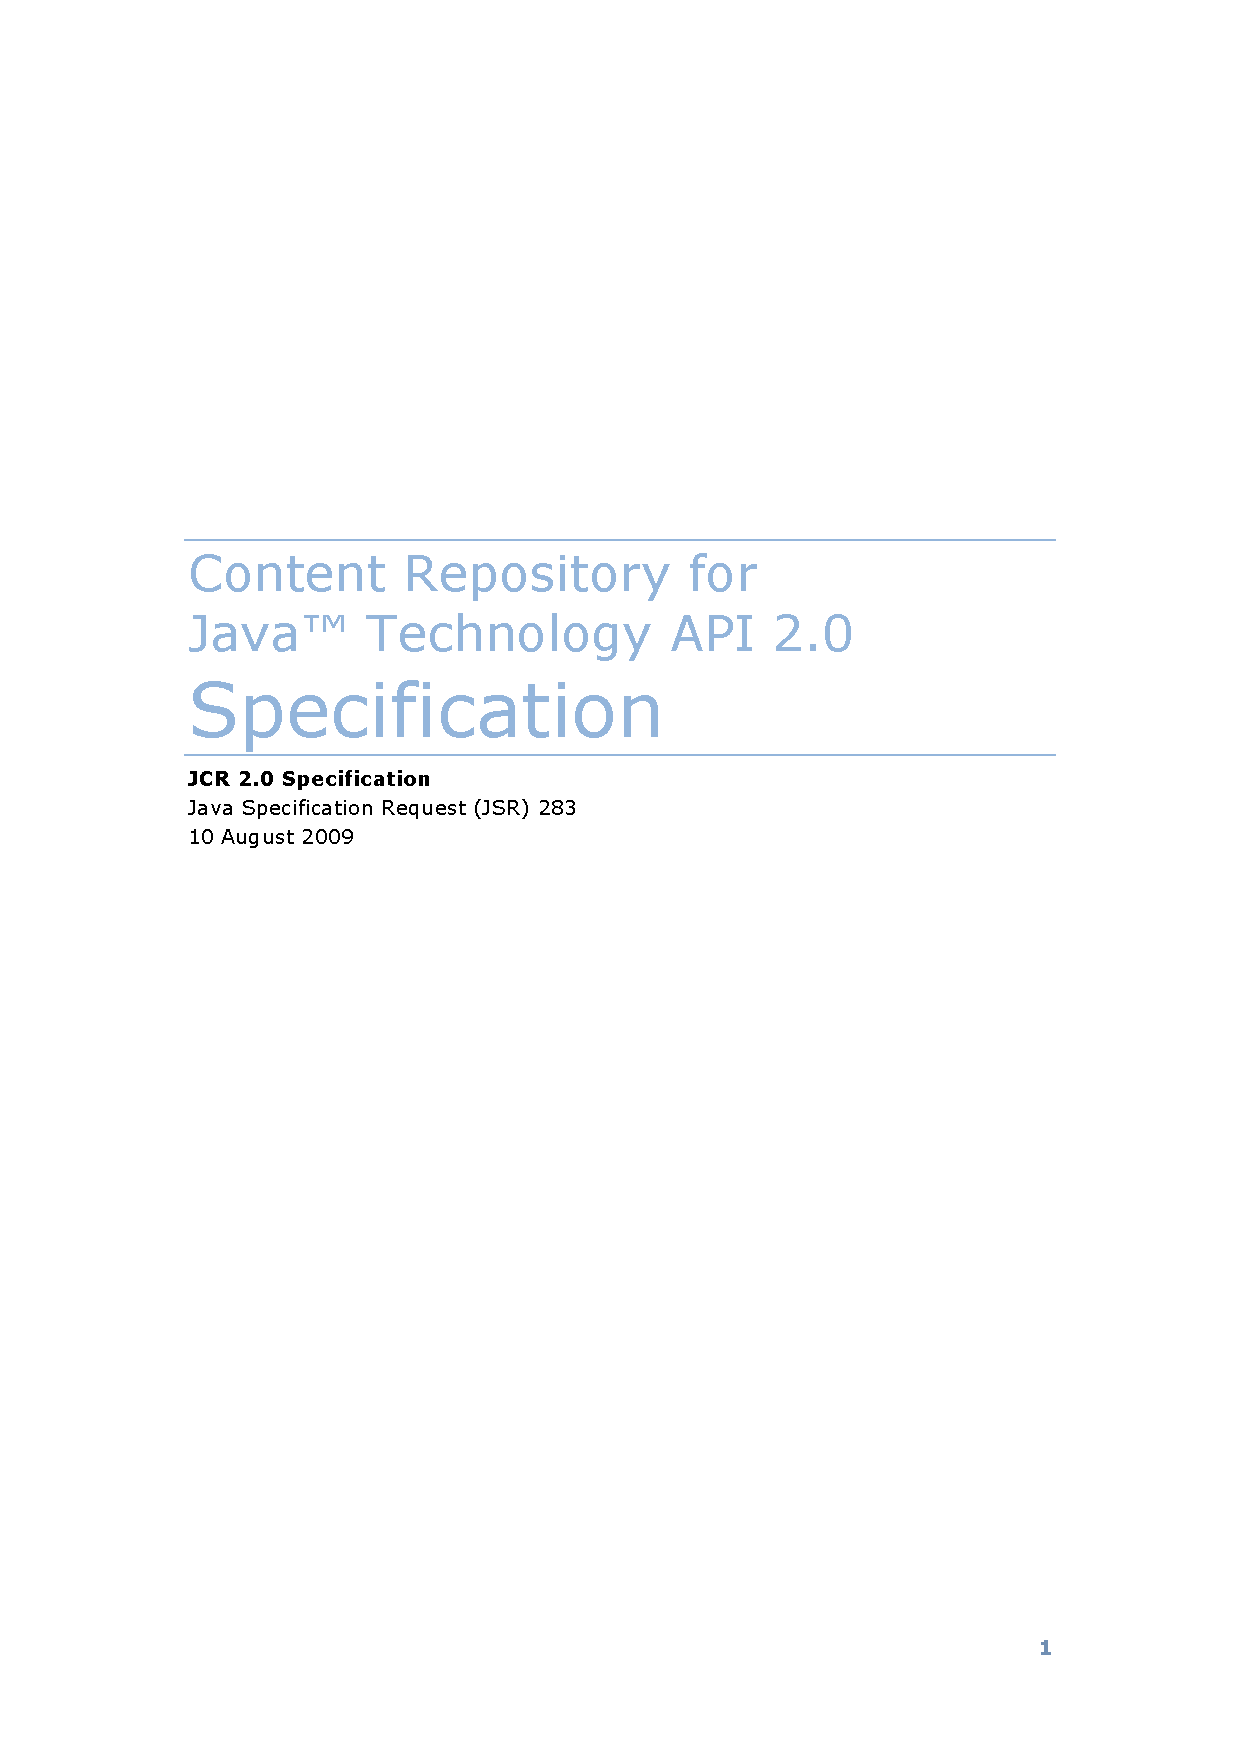
\includepdf{pdf/jcr-spec.pdf}


%%
% Diplomarbeit mit LaTeX
% ===========================================================================
% This is part of the book "Diplomarbeit mit LaTeX".
% Copyright (c) 2002-2005 Tobias Erbsland, Andreas Nitsch
% See the file diplomarbeit_mit_latex.tex for copying conditions.
%

\chapter{Installation}
\label{sec:installation}
\index{Installation|(}

\section{MiKTeX unter Windows}
\index{Installation!MiKTeX|(}

F�r Windows existiert die \DMLLaTeX-Distribution \enquote{MiKTeX}~\cite{MiKTeX}. Diese l�sst sich auf einfachste Art und Weise installieren. Die Distribution ist kostenlos und wird unter einer Open-Source-Lizenz vertrieben. Wer mag, kann sich aber auch registrieren lassen, falls er oder sie E-Mail Support w�nscht.

\subsection{Herunterladen des Setup-Programms}

Geh auf die Adresse \url{http://www.miktex.org/}. Dort findest du verschiedene Versionen des Installers, welche du herunterladen kannst.

Empfehlenswert ist hier der \enquote{Basic MiKTeX Installer}, da er die besonders h�ufig verwendeten Pakete bereits enth�lt und diese nicht mehr nachtr�glich heruntergeladen werden m�ssen. Diese Installer-Datei ist in der Version 2.7 �ber 70\,MB gro�, weshalb eine schnelle Internetverbindung sich hier als vorteilhaft erweist.

W�hle diesen Link an und lade den Installer herunter.


\subsection{Starten des Setups}

\begin{figure}[hb]
	\begin{captionbeside}{Nach dem Start des Programms erscheint dieser Screen. Du musst die Lizenzbedingungen akzeptieren.}[l]
		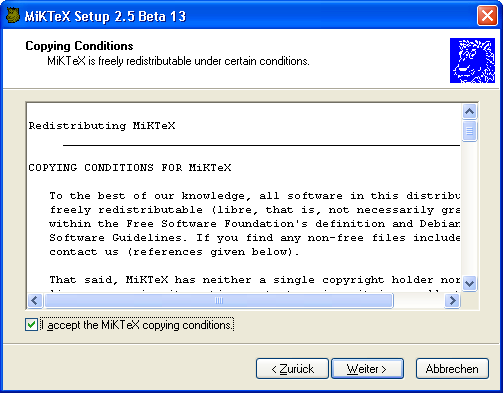
\includegraphics[width=7cm]{images/MiKTeX-install-01.png}
	\end{captionbeside}
	\label{fig:install01}
\end{figure}

\begin{figure}[hb]
	\begin{captionbeside}[Auswahl des Installationsmodus]{W�hle hier, ob nur Dein aktueller Nutzer oder alle am PC angemeldeten Nutzer MiKTeX nutzen k�nnen sollen. Letzteres ist empfehlenswert, damit es keine Probleme gibt.}[l]
		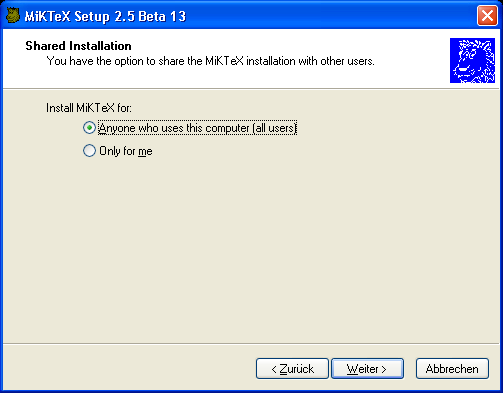
\includegraphics[width=7cm]{images/MiKTeX-install-02.png}
	\end{captionbeside}
	\label{fig:install02}
\end{figure}

\begin{figure}[hb]
	\begin{captionbeside}[Ziel der Installation w�hlen]{Hier kann das Ziel der Installation gew�hlt werden.}[l]
		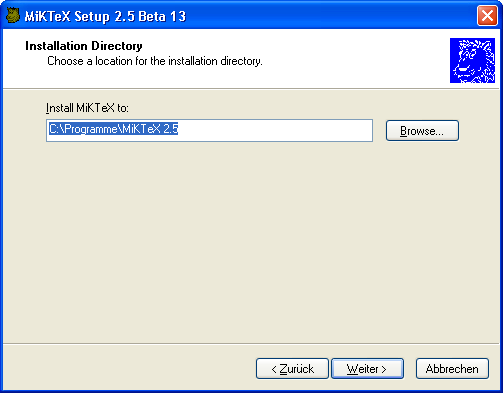
\includegraphics[width=7cm]{images/MiKTeX-install-03.png}
	\end{captionbeside}
	\label{fig:install03}
\end{figure}

\begin{figure}[hb]
	\begin{captionbeside}[Bevorzugtes Papierformat]{F�r den deutschen Sprachraum ist A4 ein sinnvoller Standard. Da Du f�r einzelne Dokumente das jeweilige Papierformat bestimmen kannst, gilt diese Einstellung nur f�r Dokumente ohne weitere Angabe.}[l]
		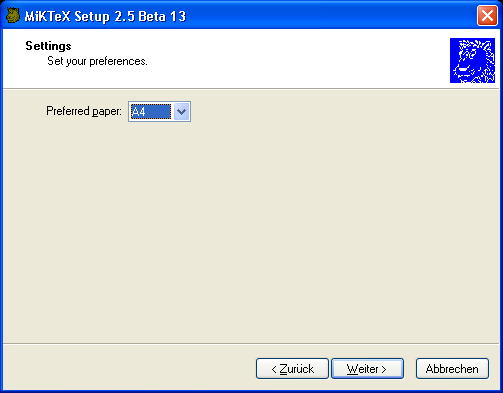
\includegraphics[width=7cm]{images/MiKTeX-install-04.png}
	\end{captionbeside}
	\label{fig:install04}
\end{figure}

\begin{figure}[th]
	\begin{captionbeside}{Der Best�tigungsscreen vor dem Start der eigentlichen Installation.}[l]
		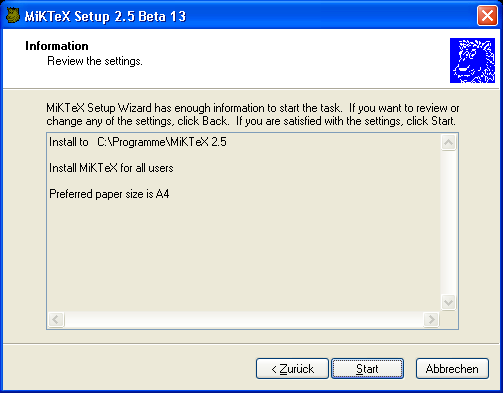
\includegraphics[width=7cm]{images/MiKTeX-install-05.png}
	\end{captionbeside}
	\label{fig:install06}
\end{figure}

\begin{figure}[th]
	\begin{captionbeside}[Die Pakete werden installiert]{Nun werden die einzelnen Pakete installiert.}[l]
		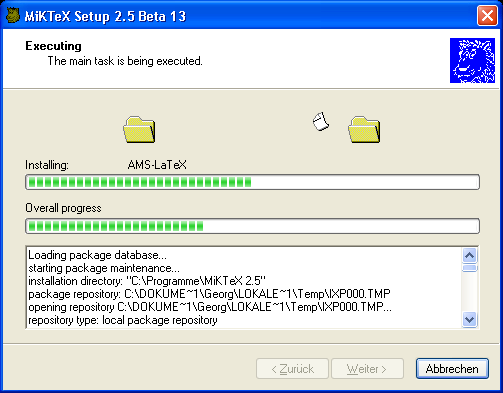
\includegraphics[width=7cm]{images/MiKTeX-install-07.png}
	\end{captionbeside}
	\label{fig:install07}
\end{figure}

\begin{figure}[th]
	\begin{captionbeside}[Das Ende des Setups]{Jetzt folgt noch ein kurzer Best�tigungsscreen und nach einem Klick auf \enquote{Close} wird das Setup beendet.}[l]
		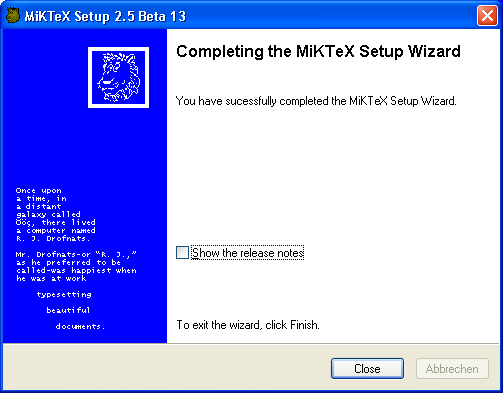
\includegraphics[width=7cm]{images/MiKTeX-install-08.png}
	\end{captionbeside}
	\label{fig:install08}
\end{figure}


\clearpage % Warten bis alle Floats ausgegeben sind.

\subsection{Herunterladen der Pakete}
\label{subsec:instpakete}

W�hrend der Benutzung von MiKTeX und TeXnicCenter wirst Du bei fehlenden Paketen gefragt, ob sie heruntergeladen werden sollen. Dies ist ein bequemer und minimalistischer Ansatz, da nur genau die Pakete installiert werden, die Du tats�chlich brauchst, und diese immer in der aktuellen Version aus dem Netz geladen werden. 

Alternativ Du kannst nat�rlich alle verf�gbaren Pakete auf einmal herunterladen -- z.B. sinnvoll, wenn Du nur vor�bergehend in der Uni breitbandig mit dem Internet verbunden bist und Festplattenplatz keinen Engpass darstellt (die allermeisten Pakete wirst Du nie verwenden, also den davon eingenommenen Platz verschwenden). Auf diese Weise stehen immer alle Pakete zur Verf�gung.

Wie du manuell einige oder alle Pakete installieren kannst, ist in den Abbildungen \ref{fig:install10} bis \ref{fig:install05b} beschrieben. 

\begin{figure}[hb]
	\begin{captionbeside}[MiKTeX Package Manager starten]{Rufe Start -- Programme -- MiKTeX -- Browse Packages auf. Der \enquote{MiKTeX Package Manager} wird gestartet. Du w�hlst die gew�nschten Pakete aus, indem Du die Steuerung-Tastste gedr�ckt h�lst und mit der Maus auf einzelne Pakete klickst, um mehrere verstreute zu markieren, bzw. indem Du die Umschalt-Tastste gedr�ckt h�lst, um mehrere benachbarte Bl�cke auszuw�hlen.)}[l]
		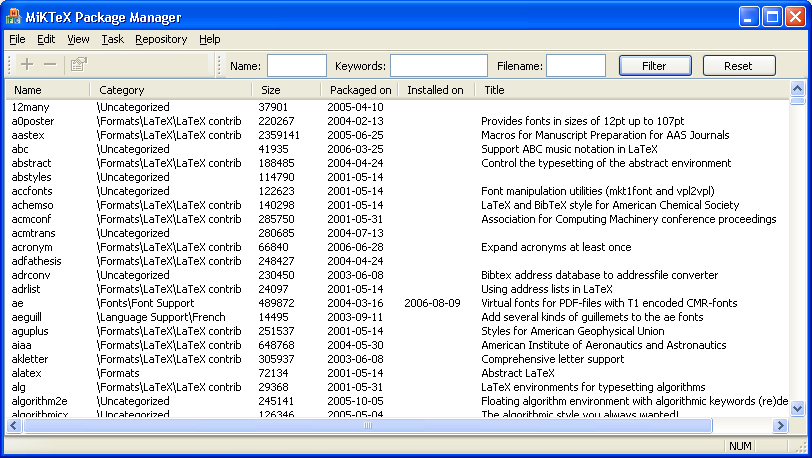
\includegraphics[width=7cm]{images/MiKTeX-packet-install-01.png}
	\end{captionbeside}
	\label{fig:install10}
\end{figure}

\begin{figure}[hb]
	\begin{captionbeside}[Auswahl der Pakete und Start der Installation]{Hast Du die gew�nschten Pakete ausgew�hlt, klickst Du auf das Plus-Icon bzw. gehst im Men� auf Task -- Install. Dieser Informationsbildschirm erscheint, den Du mit OK best�tigst.}[l]
		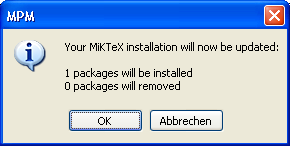
\includegraphics[width=7cm]{images/MiKTeX-packet-install-02.png}
	\end{captionbeside}
	\label{fig:install03b}
\end{figure}

\begin{figure}
	\begin{captionbeside}[Download]{Die Pakete werden aus dem Netz geladen und Dir Statusinformationen angezeigt. Klicke danach auf Close. Damit ist die Paketinstallation beendet.}[l]
		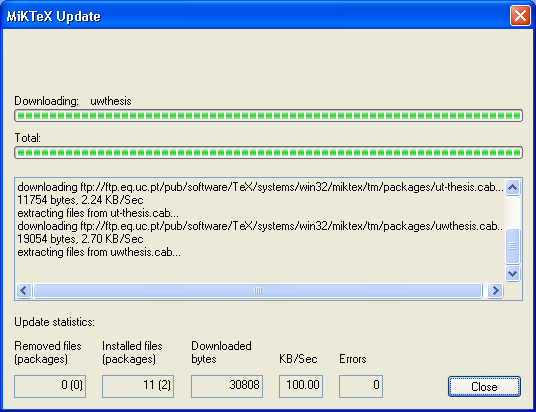
\includegraphics[width=7cm]{images/MiKTeX-packet-install-03.png}
	\end{captionbeside}
	\label{fig:install05b}
\end{figure}

\index{Installation!MiKTeX|)}

\clearpage % Warten bis alle Floats ausgegeben sind.

\section{Der Editor TeXnicCenter}
\index{Installation!TeXnicCenter|(}

Um \DMLLaTeX \ Dokumente einfach editieren zu k�nnen, bietet sich der Editor \enquote{TeXnicCenter}~\cite{TeXnicCenter} an. Dieser unterst�tzt einfache Navigation in der Dokumentstruktur, Projektverwaltung und einfachen Aufruf von \DMLLaTeX.

\subsection{Herunterladen von TeXnicCenter}

Auf der Webseite des TeXnicCenter Autors~\cite{TeXnicCenter} w�hlst du in der Navigation links \enquote{Download} an, und in der folgenden Liste, unter dem Punkt \enquote{End-User Downloads} z.\,B. \enquote{TeXnicCenter Setup, Version 1 Beta 7.01} aus. Vielleicht ist mittlerweile bereits eine neuere Version erschienen. Wichtig ist, dass du die \enquote{Binaries} in Form einer Setup \enquote{.exe} Datei herunterl�dst.

\subsection{Starten des Setups}

Starte das heruntergeladene Setup. Die Installation ist in den Abbildungen \ref{fig:install20} bis \ref{fig:install27} beschrieben.

\begin{figure}[hb]
	\begin{captionbeside}[Startscreen des Installationsassistenten]{Es erscheint der Installationsassistent.}[l]
		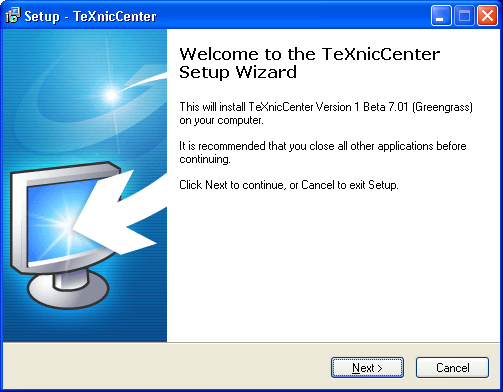
\includegraphics[width=7cm]{images/TeXnicCenter-install-01.png}
	\end{captionbeside}
	\label{fig:install20}
\end{figure}

\begin{figure}[hb]
	\begin{captionbeside}[Anzeige der GPL]{Die GNU Public License~\cite{GPL} mu� akzeptiert werden.}[l]
		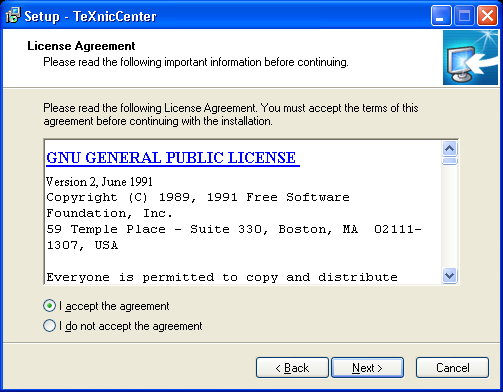
\includegraphics[width=7cm]{images/TeXnicCenter-install-02.png}
	\end{captionbeside}
	\label{fig:install21}
\end{figure}

\begin{figure}[hb]
	\begin{captionbeside}[Wahl des Installationsverzeichnisses]{Hier w�hlst du das Verzeichnis aus, in das der Editor installiert werden soll. Am Besten �bernimmst du die Vorgabe.}[l]
		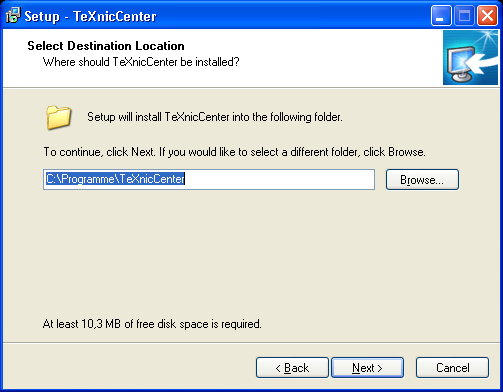
\includegraphics[width=7cm]{images/TeXnicCenter-install-03.png}
	\end{captionbeside}
	\label{fig:install22}
\end{figure}

\begin{figure}[hb]
	\begin{captionbeside}[Frage nach der Installationsart]{Jetzt wirst du nach der Installationsart gefragt. Hier w�hlst du \enquote{Typical} aus.}[l]
		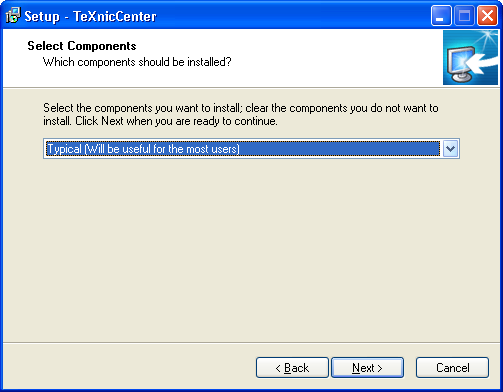
\includegraphics[width=7cm]{images/TeXnicCenter-install-04.png}
	\end{captionbeside}
	\label{fig:install23}
\end{figure}

\begin{figure}[hb]
	\begin{captionbeside}[Wahl des Namens im Startmen�]{Auch bei der Frage nach dem Namen des Eintrags ins Startmen� kannst du die Voreinstellung �bernehmen.}[l]
		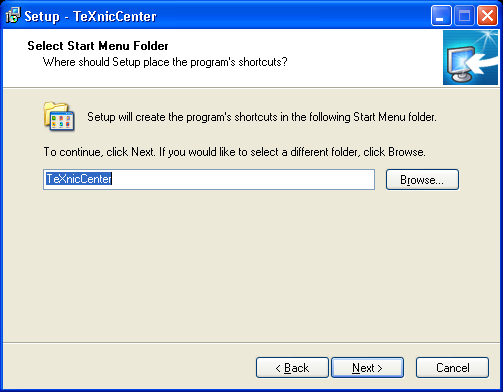
\includegraphics[width=7cm]{images/TeXnicCenter-install-05.png}
	\end{captionbeside}
	\label{fig:install24}
\end{figure}

\begin{figure}[thb]
	\begin{captionbeside}[Frage, ob ein Icon auf dem Desktop erzeugt werden soll]{Je nach Wunsch kannst du hier ein Icon auf dem Desktop und/oder einen Eintrag in das \enquote{Senden an} Kontextmen� erzeugen lassen.}[l]
		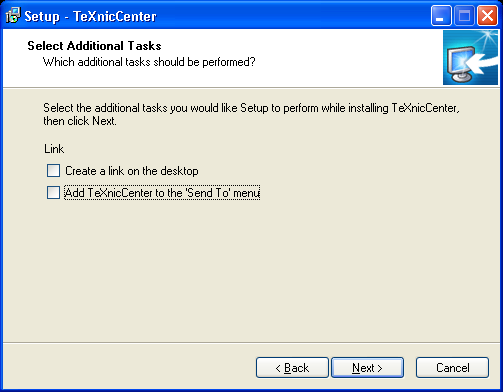
\includegraphics[width=7cm]{images/TeXnicCenter-install-06.png}
	\end{captionbeside}
	\label{fig:install25}
\end{figure}

\begin{figure}[thb]
	\begin{captionbeside}[Eine Zusammenfassung der Installation]{Jetzt folgt noch eine Zusammenfassung der Installationsangaben.}[l]
		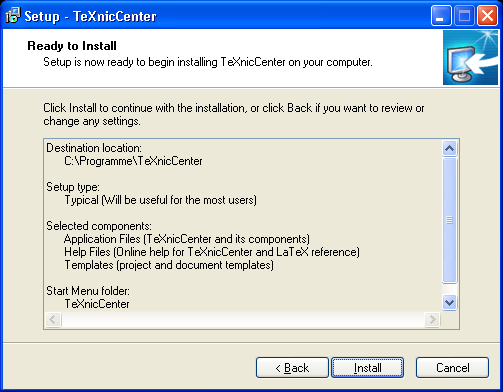
\includegraphics[width=7cm]{images/TeXnicCenter-install-07.png}
	\end{captionbeside}
	\label{fig:install26}
\end{figure}

\begin{figure}[thb]
	\begin{captionbeside}[TeXnicCenter ist installiert]{TeXnicCenter ist installiert.}[l]
		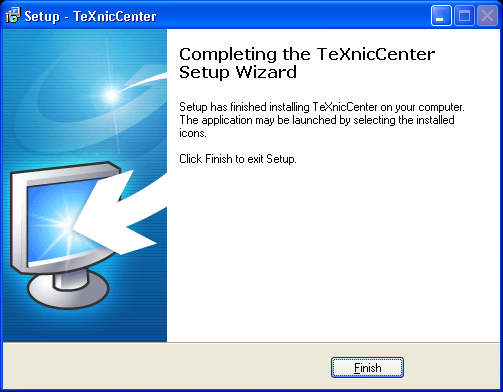
\includegraphics[width=7cm]{images/TeXnicCenter-install-08.png}
	\end{captionbeside}
	\label{fig:install27}
\end{figure}

\index{Installation!TeXnicCenter|)}

\clearpage % Warten bis alle Floats ausgegeben sind.


\section{Adobe Reader}
\index{Installation!Adobe Reader}

Jetzt solltest du noch die neuste Version des \enquote{Adobe Reader} herunterladen. Du ben�tigst mindestens die Version 5.0 (damals noch \enquote{Acrobat Reader}). Das Programm ist kostenlos und du solltest es nicht mit dem teuren \enquote{Adobe Acrobat} verwechseln, dem Programm, welches PDF-Dateien \emph{erzeugt}. Wir werden mit \DMLLaTeX \ unsere PDFs erzeugen.

Dazu gehst du auf die Webseite von Adobe~\cite{Adobe} und suchst nach einem Link \enquote{Download Adobe Reader} oder �hnlichem. Vielleicht findest du auch ein anklickbares \enquote{Get Adobe Reader} Icon. 

Du gelangst auf eine Seite mit einigen weiteren Informationen zum Adobe Reader. Weiter unten findest du drei Schritte zum Download.

Bei den Feldern im ersten Schritt w�hlst du Deutsch und dein Betriebssystem aus. Die Felder im zweiten Schritt kannst du leer lassen (empfohlen).

Nach dem Klick auf \enquote{Download} startet nach einigen Sekunden der Download von einem kleinen \enquote{Downloadmanager}. Nach dem Start von diesem Programm wird der Adobe Reader heruntergeladen und auf deinem System installiert.

\index{Installation|)}

%%
% Diplomarbeit mit LaTeX
% ===========================================================================
% This is part of the book "Diplomarbeit mit LaTeX".
% Copyright (c) 2002-2005 Tobias Erbsland, Andreas Nitsch
% See the file diplomarbeit_mit_latex.tex for copying conditions.
%

\chapter{Installation}
\label{sec:installation}
\index{Installation|(}

\section{MiKTeX unter Windows}
\index{Installation!MiKTeX|(}

F�r Windows existiert die \DMLLaTeX-Distribution \enquote{MiKTeX}~\cite{MiKTeX}. Diese l�sst sich auf einfachste Art und Weise installieren. Die Distribution ist kostenlos und wird unter einer Open-Source-Lizenz vertrieben. Wer mag, kann sich aber auch registrieren lassen, falls er oder sie E-Mail Support w�nscht.

\subsection{Herunterladen des Setup-Programms}

Geh auf die Adresse \url{http://www.miktex.org/}. Dort findest du verschiedene Versionen des Installers, welche du herunterladen kannst.

Empfehlenswert ist hier der \enquote{Basic MiKTeX Installer}, da er die besonders h�ufig verwendeten Pakete bereits enth�lt und diese nicht mehr nachtr�glich heruntergeladen werden m�ssen. Diese Installer-Datei ist in der Version 2.7 �ber 70\,MB gro�, weshalb eine schnelle Internetverbindung sich hier als vorteilhaft erweist.

W�hle diesen Link an und lade den Installer herunter.


\subsection{Starten des Setups}

\begin{figure}[hb]
	\begin{captionbeside}{Nach dem Start des Programms erscheint dieser Screen. Du musst die Lizenzbedingungen akzeptieren.}[l]
		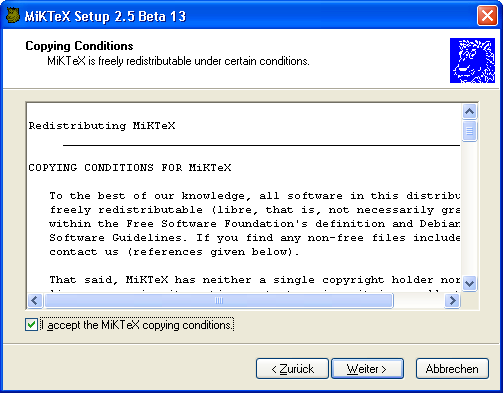
\includegraphics[width=7cm]{images/MiKTeX-install-01.png}
	\end{captionbeside}
	\label{fig:install01}
\end{figure}

\begin{figure}[hb]
	\begin{captionbeside}[Auswahl des Installationsmodus]{W�hle hier, ob nur Dein aktueller Nutzer oder alle am PC angemeldeten Nutzer MiKTeX nutzen k�nnen sollen. Letzteres ist empfehlenswert, damit es keine Probleme gibt.}[l]
		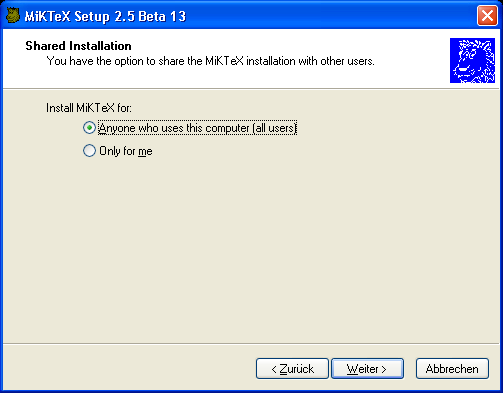
\includegraphics[width=7cm]{images/MiKTeX-install-02.png}
	\end{captionbeside}
	\label{fig:install02}
\end{figure}

\begin{figure}[hb]
	\begin{captionbeside}[Ziel der Installation w�hlen]{Hier kann das Ziel der Installation gew�hlt werden.}[l]
		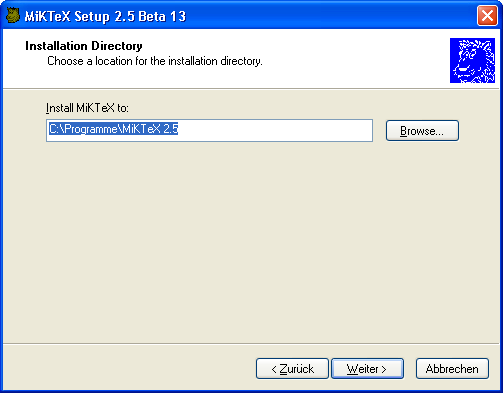
\includegraphics[width=7cm]{images/MiKTeX-install-03.png}
	\end{captionbeside}
	\label{fig:install03}
\end{figure}

\begin{figure}[hb]
	\begin{captionbeside}[Bevorzugtes Papierformat]{F�r den deutschen Sprachraum ist A4 ein sinnvoller Standard. Da Du f�r einzelne Dokumente das jeweilige Papierformat bestimmen kannst, gilt diese Einstellung nur f�r Dokumente ohne weitere Angabe.}[l]
		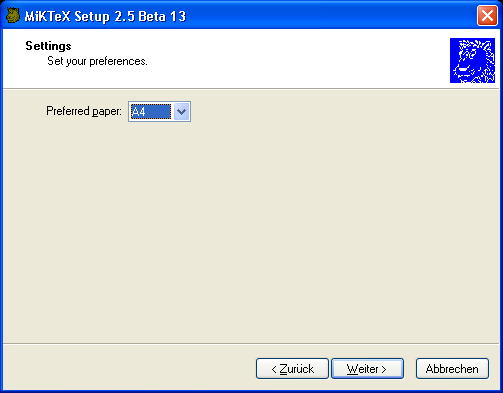
\includegraphics[width=7cm]{images/MiKTeX-install-04.png}
	\end{captionbeside}
	\label{fig:install04}
\end{figure}

\begin{figure}[th]
	\begin{captionbeside}{Der Best�tigungsscreen vor dem Start der eigentlichen Installation.}[l]
		\includegraphics[width=7cm]{images/MiKTeX-install-05.png}
	\end{captionbeside}
	\label{fig:install06}
\end{figure}

\begin{figure}[th]
	\begin{captionbeside}[Die Pakete werden installiert]{Nun werden die einzelnen Pakete installiert.}[l]
		\includegraphics[width=7cm]{images/MiKTeX-install-07.png}
	\end{captionbeside}
	\label{fig:install07}
\end{figure}

\begin{figure}[th]
	\begin{captionbeside}[Das Ende des Setups]{Jetzt folgt noch ein kurzer Best�tigungsscreen und nach einem Klick auf \enquote{Close} wird das Setup beendet.}[l]
		\includegraphics[width=7cm]{images/MiKTeX-install-08.png}
	\end{captionbeside}
	\label{fig:install08}
\end{figure}


\clearpage % Warten bis alle Floats ausgegeben sind.

\subsection{Herunterladen der Pakete}
\label{subsec:instpakete}

W�hrend der Benutzung von MiKTeX und TeXnicCenter wirst Du bei fehlenden Paketen gefragt, ob sie heruntergeladen werden sollen. Dies ist ein bequemer und minimalistischer Ansatz, da nur genau die Pakete installiert werden, die Du tats�chlich brauchst, und diese immer in der aktuellen Version aus dem Netz geladen werden. 

Alternativ Du kannst nat�rlich alle verf�gbaren Pakete auf einmal herunterladen -- z.B. sinnvoll, wenn Du nur vor�bergehend in der Uni breitbandig mit dem Internet verbunden bist und Festplattenplatz keinen Engpass darstellt (die allermeisten Pakete wirst Du nie verwenden, also den davon eingenommenen Platz verschwenden). Auf diese Weise stehen immer alle Pakete zur Verf�gung.

Wie du manuell einige oder alle Pakete installieren kannst, ist in den Abbildungen \ref{fig:install10} bis \ref{fig:install05b} beschrieben. 

\begin{figure}[hb]
	\begin{captionbeside}[MiKTeX Package Manager starten]{Rufe Start -- Programme -- MiKTeX -- Browse Packages auf. Der \enquote{MiKTeX Package Manager} wird gestartet. Du w�hlst die gew�nschten Pakete aus, indem Du die Steuerung-Tastste gedr�ckt h�lst und mit der Maus auf einzelne Pakete klickst, um mehrere verstreute zu markieren, bzw. indem Du die Umschalt-Tastste gedr�ckt h�lst, um mehrere benachbarte Bl�cke auszuw�hlen.)}[l]
		\includegraphics[width=7cm]{images/MiKTeX-packet-install-01.png}
	\end{captionbeside}
	\label{fig:install10}
\end{figure}

\begin{figure}[hb]
	\begin{captionbeside}[Auswahl der Pakete und Start der Installation]{Hast Du die gew�nschten Pakete ausgew�hlt, klickst Du auf das Plus-Icon bzw. gehst im Men� auf Task -- Install. Dieser Informationsbildschirm erscheint, den Du mit OK best�tigst.}[l]
		\includegraphics[width=7cm]{images/MiKTeX-packet-install-02.png}
	\end{captionbeside}
	\label{fig:install03b}
\end{figure}

\begin{figure}
	\begin{captionbeside}[Download]{Die Pakete werden aus dem Netz geladen und Dir Statusinformationen angezeigt. Klicke danach auf Close. Damit ist die Paketinstallation beendet.}[l]
		\includegraphics[width=7cm]{images/MiKTeX-packet-install-03.png}
	\end{captionbeside}
	\label{fig:install05b}
\end{figure}

\index{Installation!MiKTeX|)}

\clearpage % Warten bis alle Floats ausgegeben sind.

\section{Der Editor TeXnicCenter}
\index{Installation!TeXnicCenter|(}

Um \DMLLaTeX \ Dokumente einfach editieren zu k�nnen, bietet sich der Editor \enquote{TeXnicCenter}~\cite{TeXnicCenter} an. Dieser unterst�tzt einfache Navigation in der Dokumentstruktur, Projektverwaltung und einfachen Aufruf von \DMLLaTeX.

\subsection{Herunterladen von TeXnicCenter}

Auf der Webseite des TeXnicCenter Autors~\cite{TeXnicCenter} w�hlst du in der Navigation links \enquote{Download} an, und in der folgenden Liste, unter dem Punkt \enquote{End-User Downloads} z.\,B. \enquote{TeXnicCenter Setup, Version 1 Beta 7.01} aus. Vielleicht ist mittlerweile bereits eine neuere Version erschienen. Wichtig ist, dass du die \enquote{Binaries} in Form einer Setup \enquote{.exe} Datei herunterl�dst.

\subsection{Starten des Setups}

Starte das heruntergeladene Setup. Die Installation ist in den Abbildungen \ref{fig:install20} bis \ref{fig:install27} beschrieben.

\begin{figure}[hb]
	\begin{captionbeside}[Startscreen des Installationsassistenten]{Es erscheint der Installationsassistent.}[l]
		\includegraphics[width=7cm]{images/TeXnicCenter-install-01.png}
	\end{captionbeside}
	\label{fig:install20}
\end{figure}

\begin{figure}[hb]
	\begin{captionbeside}[Anzeige der GPL]{Die GNU Public License~\cite{GPL} mu� akzeptiert werden.}[l]
		\includegraphics[width=7cm]{images/TeXnicCenter-install-02.png}
	\end{captionbeside}
	\label{fig:install21}
\end{figure}

\begin{figure}[hb]
	\begin{captionbeside}[Wahl des Installationsverzeichnisses]{Hier w�hlst du das Verzeichnis aus, in das der Editor installiert werden soll. Am Besten �bernimmst du die Vorgabe.}[l]
		\includegraphics[width=7cm]{images/TeXnicCenter-install-03.png}
	\end{captionbeside}
	\label{fig:install22}
\end{figure}

\begin{figure}[hb]
	\begin{captionbeside}[Frage nach der Installationsart]{Jetzt wirst du nach der Installationsart gefragt. Hier w�hlst du \enquote{Typical} aus.}[l]
		\includegraphics[width=7cm]{images/TeXnicCenter-install-04.png}
	\end{captionbeside}
	\label{fig:install23}
\end{figure}

\begin{figure}[hb]
	\begin{captionbeside}[Wahl des Namens im Startmen�]{Auch bei der Frage nach dem Namen des Eintrags ins Startmen� kannst du die Voreinstellung �bernehmen.}[l]
		\includegraphics[width=7cm]{images/TeXnicCenter-install-05.png}
	\end{captionbeside}
	\label{fig:install24}
\end{figure}

\begin{figure}[thb]
	\begin{captionbeside}[Frage, ob ein Icon auf dem Desktop erzeugt werden soll]{Je nach Wunsch kannst du hier ein Icon auf dem Desktop und/oder einen Eintrag in das \enquote{Senden an} Kontextmen� erzeugen lassen.}[l]
		\includegraphics[width=7cm]{images/TeXnicCenter-install-06.png}
	\end{captionbeside}
	\label{fig:install25}
\end{figure}

\begin{figure}[thb]
	\begin{captionbeside}[Eine Zusammenfassung der Installation]{Jetzt folgt noch eine Zusammenfassung der Installationsangaben.}[l]
		\includegraphics[width=7cm]{images/TeXnicCenter-install-07.png}
	\end{captionbeside}
	\label{fig:install26}
\end{figure}

\begin{figure}[thb]
	\begin{captionbeside}[TeXnicCenter ist installiert]{TeXnicCenter ist installiert.}[l]
		\includegraphics[width=7cm]{images/TeXnicCenter-install-08.png}
	\end{captionbeside}
	\label{fig:install27}
\end{figure}

\index{Installation!TeXnicCenter|)}

\clearpage % Warten bis alle Floats ausgegeben sind.


\section{Adobe Reader}
\index{Installation!Adobe Reader}

Jetzt solltest du noch die neuste Version des \enquote{Adobe Reader} herunterladen. Du ben�tigst mindestens die Version 5.0 (damals noch \enquote{Acrobat Reader}). Das Programm ist kostenlos und du solltest es nicht mit dem teuren \enquote{Adobe Acrobat} verwechseln, dem Programm, welches PDF-Dateien \emph{erzeugt}. Wir werden mit \DMLLaTeX \ unsere PDFs erzeugen.

Dazu gehst du auf die Webseite von Adobe~\cite{Adobe} und suchst nach einem Link \enquote{Download Adobe Reader} oder �hnlichem. Vielleicht findest du auch ein anklickbares \enquote{Get Adobe Reader} Icon. 

Du gelangst auf eine Seite mit einigen weiteren Informationen zum Adobe Reader. Weiter unten findest du drei Schritte zum Download.

Bei den Feldern im ersten Schritt w�hlst du Deutsch und dein Betriebssystem aus. Die Felder im zweiten Schritt kannst du leer lassen (empfohlen).

Nach dem Klick auf \enquote{Download} startet nach einigen Sekunden der Download von einem kleinen \enquote{Downloadmanager}. Nach dem Start von diesem Programm wird der Adobe Reader heruntergeladen und auf deinem System installiert.

\index{Installation|)}


%%
% Diplomarbeit mit LaTeX
% ===========================================================================
% This is part of the book "Diplomarbeit mit LaTeX".
% Copyright (c) 2002, 2003, 2005 Tobias Erbsland, Andreas Nitsch
% See the file main.tex for copying conditions.
%

\chapter{Konfiguration}
\index{Konfiguration}

\section{MiKTeX}
\index{Konfiguration!MiKTeX}

Die \DMLLaTeX-Distribution \enquote{MiKTeX} musst du nicht konfigurieren. Es handelt sich dabei au�er bei dem DVI-Betrachter um Kommandozeilentools. Du solltest nur den Editor TeXnicCenter einrichten (siehe dazu \ref{sec:KonfigurationTeXnicCenter}).

Du solltest jedoch mit dem \enquote{MiKTeX Update Wizard} alle Pakete der Distribution auf den neuesten Stand zu bringen. Wie du das machst beschreibt die Hilfe zu MiKTeX ausf�hrlich\footnote{\enquote{User Guide}$\Rightarrow$\enquote{Maintenance}$\Rightarrow$\enquote{Installing Updates}}.

\section{TeXnicCenter}
\label{sec:KonfigurationTeXnicCenter}
\index{Konfiguration!TeXnicCenter}

\subsection{TeXnicCenter f�r die Verwendung mit MiKTeX konfigurieren}

Nach dem ersten Start erscheint der Einrichtungsassistent. Falls du diesen bereits abgebrochen hast, kann man Ihn �ber das Men� \enquote{Ausgabe}, \enquote{Ausgabeprofile definieren...} und dort in dem Dialog \enquote{Assistent} links unten erneut aufrufen. Doch wie schon gesagt, der Assistent startet normalerweise beim ersten Start vom TeXnicCenter automatisch.

\begin{figure}[hb]
	\begin{captionbeside}[Start des Konfigurations-Assistenten]{Der Assistent Startet mit dem diesem Screen}[l]
		\includegraphics[width=7cm]{images/konfiguration01.png}
	\end{captionbeside}
	\label{fig:konfiguration01}
\end{figure}

\begin{figure}[hb]
	\begin{captionbeside}[Frage, f�r welche Distribution TeXnicCenter eingerichtet werden soll]{Hier teilt dir der Installationsassistent mit, dass er die installierte \enquote{MiKTeX}-Distribution erkannt hat und fragt, ob er den Editor mit dieser \DMLLaTeX-Distribution konfigurieren soll. Du w�hlst nat�rlich \enquote{Ja}.}[l]
		\includegraphics[width=7cm]{images/konfiguration02.png}
	\end{captionbeside}
	\label{fig:konfiguration02}
\end{figure}

\begin{figure}[ht]
	\begin{captionbeside}[Optionale Eingabe eines Postscript Betrachters]{Jetzt wirst du nach einem Programm zur PostScript-Betrachtung gefragt. Hier l�sst du alle Felder leer.}[l]
		\includegraphics[width=7cm]{images/konfiguration03.png}
	\end{captionbeside}
	\label{fig:konfiguration03}
\end{figure}

\begin{figure}[ht]
	\begin{captionbeside}[Anzeige der drei generierten Profile]{Der TeXnicCenter-Assistent teilt dir mit, das er drei Profile generieren wird. Ein DVI-, ein PostScript- und ein PDF-Profil. Wir werden nur das PDF-Profil verwenden.}[l]
		\includegraphics[width=7cm]{images/konfiguration04.png}
	\end{captionbeside}
	\label{fig:konfiguration04}
\end{figure}

\clearpage % Warten auf alle Floats

\subsection{Die Rechtschreibpr�fung}
\index{Rechtschreibprufung@Rechtschreibpr�fung}

Ein sehr sch�nes und n�tzliches Feature, welches dir TeXnicCenter bietet ist die Rechtschreibpr�fung. W�hle dazu im Men� \emph{Extras} den Punkt \emph{Optionen} aus. In dem Dialog, der sich ge�ffnet hat w�hlst du den Reiter \emph{Rechtschreibung} aus. Dort kannst du die verschiedenen Optionen der Rechtschreibpr�fung einstellen.

Die m�glichen Einstellparameter sind selbsterkl�rend, was du sehr gut in Abbildung \ref{fig:rechtschreibung} siehst.

\begin{figure}
	\centering
		\includegraphics[width=0.60\textwidth]{images/rechtschreibung.png}
	\caption{Konfigurationsm�glichkeiten der Rechtschreibpr�fung}
	\label{fig:rechtschreibung}
\end{figure}

Falls eine gew�nschte Sprache fehlt, kannst du zus�tzliche W�rterb�cher installieren. W�rterb�cher diverser Sprachen, auch der neuen und alten deutschen Rechtschreibung, findest du unter folgender Internetadresse zum kostenlosen Download:

\url{http://lingucomponent.openoffice.org/download\_dictionary.html}

Entpacke die in der heruntergeladenen ZIP Datei enthaltenen Dateien in das Unterverzeichnis \enquote{Language} deiner TeXnicCenter Installation. Die TeXnicCenter Installation findest du normalerweise in dem folgenden Verzeichnis:

\verb|C:\Programme\TeXnicCenter\Language|




%\chapter{Grundlagen}

\section{Entwicklung mit Ruby on Rails}

2004 arbeitete der dänische Programmierer David Heinemeier Hansson an der Umsetzung eines webbasierten Projektmanagement-Tools mit dem Namen Basecamp\footnote{Projekt-Homepage: \href{http://basecamphq.com/}{http://basecamphq.com/}}. Die bei der Realisierung des Projektes umgesetzten Teilkomponenten extrahierte er später und veröffentlicht sie 2005 als Framework unter dem Namen Ruby on Rails.
Ruby on Rails basiert dabei auf der objektorientierten Programmiersprache Ruby und ermöglicht die schnelle Entwicklung von Webanwendungen nach dem MVC-Paradigma (Kapitel sec:mvc).
\newline
6 Jahre später (die zahlreiche Änderungen und Verbesserungen am Framework ermöglichten) beschreibt sich das Ruby on Rails-Projekt selbst mit folgenden plakativen Worten:
\begin{quote}
Ruby on Rails is an open-source web framework that’s
optimized for programmer happiness and sustainable
productivity. It lets you write beautiful code by
favoring convention over configuration. \cite[vgl.][]{RailsStatement}
\end{quote}

Diese subjektive Aussage der Rails-Kernentwickler bezieht sich dabei auf viele Ansätze und Entwicklungsabläufe, die innerhalb des Frameworks umgesetzt werden.
Im folgenden Abschnitt sollen die mit dieser Aussage angedeuteten wichtigsten Prinzipien, Paradigmen und Programmierabläufe des Frameworks zusammengefasst werden, um auf dieser Grundlage eine nichtfunktionale Betrachtung der Rails WCMS in Kapitel 4 zu ermöglichen. Auf die Themen Rest (Kapitel \ref{grundrest}) und Middleware (Kapitel \ref{grundrack}) wird dabei ausführlicher eingegangen, um für die in Kapitel 5 umgesetzten Lösungsvorschläge entsprechendes Vorwissen zu schaffen.
\newline
\newline
Für eine umfassende Einführung in Rails werden \cite{RubyMetaprogramming2010} und \cite{EnterpriseRails} empfohlen.

\subsection{Don't-Repeat-Yourself (DRY)}
Zur Optimierung der Entwicklungvorgänge innerhalb des Frameworks propagiert Rails den Grundsatz des DRY (Don't-Repeat-Yourself). Dabei sollen Redundanzen, d.h. die wiederholte Angabe identischer Informationen jeglicher Art vermieden werden. So kann sichergestellt werden, dass sich Änderungen an einer zentralen Stelle im System (z.B. Quellcode) in der gesamten Anwendung auswirken und Duplikate nicht mehrfach angepasst werden müssen.
\subsection{Convention over Configuration}
Viele Web Frameworks müssen vor ihrer Nutzung erst mit Hilfe zahlreicher Konfigurationsdateien und Parametereinstellungen zu einem lauffähigen Gesamtsystem zusammengebaut werden\footnote{Rails bezeichnet diese Art der Frameworks mit ihrem Konfigurations-Overhead oft als \emph{enterprisy}. Dies bedeutet jedoch nicht, das Rails für Anwendungsumsetzungen im Enterprise-Bereich ungeeignet ist. \citep[vgl.][]{enterprisy}.}. Abbildung \ref{spring} zeigt beispielhaft solch eine Konfigurationsdatei innerhalb des Java Application Frameworks Spring\footnote{Projektseite: \href{http://www.springsource.org/}{http://www.springsource.org/}}:

\lstinputlisting[label=spring,language=xml, caption=Konfigurationsdatei im Java Spring Framework]{code/spring.xml}
Um diesen zusätzlichen und zeitraubenden Aufwand vor der eigentlichen Arbeit mit einem Framework zu vermeiden, definiert Rails zahlreiche Konventionen, die es erlauben, sofort mit der Entwicklungsarbeit zu beginnen. U.a. werden folgende Festlegungen getroffen:

\begin{itemize}
\item
Informationen zur Datenbankverbindung der Anwendung müssen in der Datei database.yml im Unterordner config hinterlegt werden
\item
Der Klassenname eines Domainenmodells wird im Singular erwartet, der dazu korrespondierende Tabellename in der Datenbank hingegen im Plural z.B. Domainenmodell Project => Datenbanktabelle projects
\item
Der Primärschlüssel in einer Datanbanktabelle muss vom Typ Integer sein und den Namen ID besitzen
\item
Rails erwartet eine definierte Ordnerstrukur für Controller, Domainmodell und Views\footnote{Eine Erklärung zu Model-View-Controller folgt in Abschnitt \ref{sec:mvc}}
\end{itemize}
Für den produktiven Einsatz des Frameworks müssen diese daher erlernt und akzeptiert werden, was dazu führt, dass Rails häufig als \emph{opinionated software\footnote{Eine ausführliche Stellungnahme von Rails-Erfinder David Heinemeier Hansson zu diesem Thema gibt es unter: \href{http://www.linuxjournal.com/article/8686}{http://www.linuxjournal.com/article/8686}}} (starr- und eigensinnige Software) bezeichnet wird.

Ein Abweichen von den definierten Konventionen ist jederzeit möglich, erhöht jedoch den Aufwand des Entwicklers.

\subsection{Model-View-Controller (MVC)}
\label{sec:mvc}
Für Software-Designer ist es  eine gebräuchliche Technik, komplexe Software-Systeme durch Schichtenbildung in einzelne Bestandteile zu zerlegen \citep[Kapitel 1]{FowlerPatterns}. Das Ruby on Rails Framework baut ebenfalls auf einem Mehr-Schichten-Architektur-Modell auf. Zusätzlich kommt eine für das Rails-Framework spezifische Implementierung des bereits 1979 von dem Norweger Trygve Mikkjel Heyerdahl entwickelten Model-View-Controller-Paradigmas zum Einsatz\footnote{In der Fachliteratur wird das MVC-Paradigma häufig auf die Schichtenarchitektur einer Anwendung übertragen \cite[S. 544 ff.]{objekt}. Tatsächlich betrifft MVC in seiner  ursprünglichen Form nur die Präsentationsschicht einer Webanwendung.}.
Abbildung \ref{fig:mvcimage} charakterisiert den Ablauf einer Anfrage (Request) an eine Rails-Anwendung innerhalb des Client-Server-Modells sowie die Komponenten Model, View und Controller, die eine exakte Trennung der Verantwortungsbereiche in einer Rails-Anwendung sicherstellen:

\begin{figure}[!h]
\begin{center}
\includegraphics[scale=0.4]{images/analyse/mvc.png}
%\caption{Nutzung verschiedener Programmiersprachen auf Servern}{Quelle: \citep{w3techs}}


\caption[Verarbeitung einer Anfrage innerhalb des Rails-Frameworks]{Verarbeitung einer Anfrage (Client-Server-Modell) innerhalb des Rails-Frameworks. Quelle: \citep[Seite 6]{railsmvc}}
\label{fig:mvcimage}
\end{center}
\end{figure}

\begin{enumerate}
\item
Anfrage eines Clienten
\item
An Hand der im Rails-Routing definierten Einträge wird die Anfrage eines Clienten an den registrierten Controller weitergeleitet
\item
Der Controller steuert den Ablauf innerhalb der Anwendung. Dabei greift er über ein Model auf benötigte Daten in einem Speicher (z.B. relationale Datenbank) zu und stellt diese dem View-Layer zur Verfügung. Es ist auch möglich, dass der Controller die Anfrage an einen anderen Controller weiterleitet (Redirects). Im Gesamtkonzept von Rails enthält der Controller die Programmlogik der Anwendung.
\item
Als Model werden in Rails Ruby-Klassen bezeichnet, die einen Zugriff auf relationale Datenbanken oder andere Datenspeicher ermöglichen \citep[vgl.][]{Rails2}. Es bildet innerhalb der Anwendung die zugrundliegende Datenstruktur ab.
%\citep[vgl.][]{Rails2}
\item
Der View-Layer (Sicht- oder Darstellungsschicht) bereitet die durch den Controller zur Verfügung gestellten Daten in der angeforderten Darstellungsform auf und gibt das Ergebnis der Anfrage aus. So wird je nach spezifiziertem Format z.B. eine HTML- oder XML-Datei erzeugt. Ein View repräsentiert somit die Darstellung einer bestimmten Datenstruktur (Model).
\item
Das Ergebnis der Anfrage (die Ausgabe des View) wird vom Framework an den Server übermittelt und von dort an den Clienten ausgeliefert (Response). Der Kommunikationsprozess mit dem Rails-Framework ist damit abgeschlossen.
\end{enumerate}



\subsection{REST}
\label{grundrest}
Innerhalb einer Web-Applikation erfolgt der Austausch zwischen Server und Client durch die Nutzung des HTTP-Protokolls. Dabei wird eine Anfrage (Request) an einen Server geschickt, bearbeitet und eine entsprechende Antwort (Response) mit den angeforderten Inhalten zurückliefert. Ein Großteil der Webanwendungen interpretiert dabei die im HTTP-Protokoll definierten Methoden GET und POST:

\begin{description}
\item[GET]
Anforderung an den Server, eine über die Adresszeile des Browsers angegebene Ressource zurückzuliefern. Es können zusätzlich Argumente an die angeforderte URL angehängt werden.
\item[POST]
Mit Hilfe dieser Methode ist es möglich, große Datenmengen aus z.B. Formularen an einen Webserver zu verschicken. Die übergebenen Informationen werden dabei im sogenannten Body der Anfrage codiert mitverschickt und somit im Vergleich zu GET nicht in der URL sichtbar\footnote{Ein Post-Request findet vor allem bei der Übermittlung von Formularen innerhalb eines Browsers Verwendung.}.
\end{description}


REST, ein Akronym für \textbf{RE}epresentational \textbf{S}tate \textbf{T}ransfer, erweitert die in  traditionellen Webanwendungen üblichen GET und POST um die ebenfalls im HTTP-Standard enthaltenen Methoden PUT und DELETE:
\begin{comment}
\begin{description}
\item[GET]
Abfrage einer Ressource unter der angegebenen URL mit  anschließender Darstellung
\item[POST]
Erstellung einer neuen Ressourcen an Hand der in der Anfrage übermittelten Daten, Realisierung durch Formulare auf Clientseite
\item[PUT]
Überschreiben der angeforderten Ressource mit den in der Anfrage neu übermittelten Daten
\item[DELETE]
Löschen der beschriebenen Ressource
\end{description}
\end{comment}

\begin{description}
\item[PUT]
	Die Verwendung der PUT-Methode zeigt die Neuanlage der in einer	Anfrage spezifizierten Ressource an
\item[DELETE]
	Die Verwendung dieser Methode signalisiert dem Server, die angegebene Ressource auf dem Server zu löschen.
\end{description}
Da aktuelle Browser nur GET- und POST-Anfragen zuverlässig unterstützen, müssen entsprechende Anfragen zum Löschen und Verändern einer Ressource mit Hilfe von zusätzlichen Attributen in der Anfrage simuliert werden\footnote{Das Rails Framework fügt  innerhalb von Formularen automatisch einen versteckten Parameter \emph{\_method} in die Anfrage, die den Namen der gewünschten HTTP-Metode (DELETE oder PUT) enthält. Im Framework wird dieser Parameter ausgelesen und ein entsprechendes Routing zur geforderten Controller-Action eingeleitet.}. Das folgende Beispiel stellt das von Rails definierte Standard-Routing einer als \emph{restful} angelegten Ressource Projekt dar\footnote{REST wird nicht über einen entsprechend formulierten Standard definiert. Vielmehr kann es als Programmierparadigma innerhalb von Web-Anwendungen verstanden werden, die eine Ansammlung von Best-Practices darstellen \cite{restful}.}.

\begin{table}[!h]
\caption{Rails Routing der Rest-Ressource Projekt}
\center
\begin{tabular}[!ht]{|p{2cm}|p{3cm}|p{3cm}|p{6cm}|}
\hline
HTTP-Methode & Anfragepfad & Ausgelöste Aktion im Controller & Wirkung\\
\hline
GET	& /projects & index & Anzeige aller vorhandenen Projekte\\
\hline
GET	& /projects/new	& new &	Anzeige eines HTML-Formulars zum erstellen eines neuen Projektes\\
\hline
POST & /projects & create & Erstellt ein neues Projekt mit den übermittelten Daten\\
\hline
GET & /projects/:id &	show &	Anzeige eines Projektes mit der zugeordneten ID\\
\hline
GET	& /projects/:id/edit & edit & Anzeige eines HTML-Formulars zum Bearbeiten eines bestehenden Projektes\\
\hline
PUT	& /projects/:id &	update & Aktualisierung eines bestimmten Projektes mit den übermittelten Daten\\
\hline
DELETE & /projects/:id &	destroy &	Löschung des Projektes mit der angegebenen ID\\
\hline
\end{tabular}
\end{table}

\begin{table}[!ht]
\caption{Vergleich zwischen Rest-konformen und klassischen Rails-URL's}
\label{tab.restnonrest}
\center
\begin{tabular}[!ht]{|l|l|l|}
\hline
Aktion & normale URL & 	REST URL in Rails \\
\hline
show &	/projects/show/12 &	/projects/12 \\
\hline
delete & /projects/destroy/123 & /projects/123 \\
\hline
update & /projects/update/123 &	/projects/123 \\
\hline
create & /projects/create & /projects \\
\hline
\end{tabular}
\end{table}

Tabelle \ref{tab.restnonrest} zeigt noch einmal die Trennung zwischen Ressource und Aktion innerhalb einer in Rails definierten REST-Ressource Projekt. Eine ausführliche Beschreibung von REST und dessen Realisierung liefert \cite{restful}.

\newpage
\subsection{Rack und Middleware}
\label{grundrack}
Rails ist innerhalb der Ruby-Gemeinde nicht das einzigste existierende Webframework. Mit den Projekten Sinatra\footnote{Projektseite: \href{http://www.sinatrarb.com/}{http://www.sinatrarb.com/}}, Merb\footnote{Projektseite: \href{http://www.merbivore.com/}{http://www.merbivore.com/}}, Camping\footnote{Projektseite: \href{http://camping.rubyforge.org/}{http://camping.rubyforge.org/}} und Ramaze\footnote{Projektseite: \href{http://ramaze.net/}{http://ramaze.net/}} stehen weitere Alternativen mit unterschiedlichen Ansätzen und Funktionsumfängen zur Verfügung.
Bei der Implementierung dieser Frameworks müssen Entwickler wiederholt Adapter\footnote{} (Handler) zur Ansteuerung verschiedener Webserver entwickeln. Durch Rack\footnote{Projektseite: \href{http://rack.rubyforge.org/}{http://rack.rubyforge.org/}}, einem Ruby Webserver Interface, lässt sich die wiederholte Implementierung solcher Adapter in den einzelnen Frameworks vermeiden.
\begin{figure}[!h]
\begin{center}
\includegraphics[scale=0.6]{images/rack/rack.pdf}
\caption{Rack als Vermittler zwischen Server und Ruby-Webframeworks}
\label{rackschema}
\end{center}
\end{figure}


Damit Server und Frameworks untereinander kommunizieren können, muss eine Rack-Anwendung bestimmte Methoden implementieren und ein bestimmtes Rückgabeformat einhalten. An Hand des Beispiels in \ref{rack} sollen diese formalen Kriterien beschrieben werden:

\lstinputlisting[label=rack,language=Ruby, caption=Beispiel für eine einfache Rack-Anwendung]{code/rack.rb}

\begin{description}
\item[Zeile 6-8]\mbox{~}\\*
Initialisierung der Rack-Anwendung MyRackApp unter Angabe eines zuvor übergebenen Namen (\emph{Rack} in Zeile 15).
\item[Zeile 10-12]\mbox{~}\\*
Implementierung der für eine Rack-Anwendung notwendigen Methode \emph{call}. Diese wird vom Webserver beim Start einer Anfrage aufgerufen und muss als Antwort (Rückgabewert) einen Ruby-Hash mit den folgenden Informationen zurückliefern:
\begin{description}
\item[Status]\mbox{~}\\*
Angabe des HTTP-Statuscode, \emph{200} bedeutet in diesem Beispiel eine erfolgreiche Ausführung der Anfrage am Server\footnote{Die HTTP-Statuscodes sind im HTTP-Protokoll definiert und können u.a. unter folgender Quelle eingesehen werden: \href{http://www.w3.org/Protocols/rfc2616/rfc2616-sec10.html}{http://www.w3.org/Protocols/rfc2616/rfc2616-sec10.html}}
\item[Header]\mbox{~}\\*
Angabe von im HTTP-Protokoll definierten Header-Informationen,  im Beispiel wird ein einfaches Textdokument (\emph{text/plain}) zurückgeliefert
\item[Response]\mbox{~}\\*
Die Antwort der Rack-Anwendung, im Beispiel wird ein String \emph{Hello Rack!} an den Server übergeben und von diesem ausgeliefert.
\end{description}

Beim Aufruf der Methode \emph{call} (Zeile 15) übergibt der Server eine Variable \emph{env}, die alle wichtigen Informationen über die Serverumgebung und Anfrageparameter enthält.
\item[Zeile 15]\mbox{~}\\*
Start des Mongrel Webservers und Initialisierung der Rack-Anwendung \emph{MyRackApp}.
\end{description}

Bei einem Aufruf der Adresse \emph{localhost:3001} in einem Browser wird vom gestarteten Mongrel-Server der Rückgabewert der Methode \emph{call} ausgegeben (Abb. \ref{rackoutput}).

\begin{figure}[!ht]
\begin{center}
\includegraphics[scale=0.6]{images/rack/outputrack2.png}
\caption{Ausgabe der Rack-Anwendung MyRackApp im Browser}
\label{rackoutput}
\end{center}
\end{figure}

Durch die Nutzung von Rack ergeben sich im Bereich der Ruby Webframeworks folgende Vorteile:

\begin{itemize}
\item
Vereinfachung der Webframework-Entwicklung: Ein Framework, das Rack unterstützt, kann sofort von allen anderen rack-unterstützenden Webservern verwendet werden.
\item
Vereinfachung der Serverentwicklung: Ein rack-unterstützender Server kann sofort mit allen rack-basierten Webframeworks eingesetzt werden.
\item
Keine Codeduplizierung durch wiederholte Entwicklung von Server-Adaptern innerhalb der verschiedenen Ruby Webframeworks
\item
Rack beinhaltet Handler für die meist verbreitesten Webserver in Ruby (Abbildung \ref{rackschema})
\end{itemize}


Darüber hinaus ist es  möglich, einzelne Rack-Anwendungen hintereinander zu schalten und so ein Filtersystem für ankommende Anfragen und ausgehende Antworten vor dem eigentlichen Webframework zu realisieren.
Diese Anwendungen werden Rack-Middlewares genannt und können in einer Rails-Anwendung in der Startkonfiguration des Frameworks eingebunden werden. So kann das Ein- und Ausgabeverhalten des Railsframeworks gezielt verändert werden, da die einzelnen Rack-Anwendungen entscheiden, ob der nächste Filter (die nächste registrierte Rack-Middleware) oder eine vorzeitige Anwort an den Server geschickt werden soll.

%\lstinputlisting[label=middlewarestack,language=Ruby, caption=Registrierung verschiedener Middlewares in einer Rails 3 Anwendung]{code/middleware.rb}
Das Rails-Framework steht selbst am Ende der Filterliste und ist im Kontext von Rack selbst als Rack-Anwendung eingebunden (Abb. \ref{rackmiddlewares}).
\begin{figure}[!ht]
\begin{center}
\includegraphics[scale=0.5]{images/rack/middlewares.png}
\caption{Möglichkeiten der unterschiedlichen Rückgabewerte durch Rack Middlewares und Rails}
\label{rackmiddlewares}
\end{center}
\end{figure}
Eine detaillierte Beschreibung von Rack und der Einrichtung eines komplexen Filtersystems\footnote{Rack stellt häufig verwendete Middlewares für verschiedene Aufgabenbereiche zur Verfügung. Die Projektseite ist unter folgender Adresse verfügbar: \href{https://github.com/rack/rack-contrib}{https://github.com/rack/rack-contrib}} in einer Rails-Anwendung liefern \cite{rack} und \cite{railsguiderack}.

\subsection{Generatoren}
\label{sec:railsgeneratoren}
Das Ruby on Rails Framework unterstützt mit Hilfe sogenannter Generatorskripte die automatische Erzeugung von funktionsfähigem Quellcode. Der folgende Scaffold-Generator\footnote{Scaffold kann in diesem Zusammenhang mit dem Wort Grundgerüst übersetzt werden.} erstellt z.B. nach dessen Initialisierung ein komplett funktionsbereites Codegerüst für die in Rails benötigten MVC-Komponenten einer Ressource \emph{Projekt}.

\begin{lstlisting}[caption=Aufruf des Generators zur Erstellung einer MVC-Ressource Projekt]
rails g scaffold project name:string description:text
\end{lstlisting}

\lstinputlisting[label=scaffold,language=Ruby, caption=Auflistung der erstellten Dateien des Scaffold-Generators]{code/scaffold.txt}

\section{Web Content Management, Content Life Cycle und Web-Publishing}
\label{sec:webpublishing}
Der in der einschlägigen Literatur bereits mehrfach thematisierte Anstieg von Content\footnote{
\glqq Unter dem Begriff des \flqq Contents\frqq~ werden alle Inhalte verstanden, die in einem CMS verwaltet werden und die im engeren Sinne für die Erstellung von Dokumenten und Publikationen verwendet werden. Darunter fallen alle textuellen und (audio-)visuellen Informationen [..] \citep[S. 297]{TechnischeDok}
} erfordert innerhalb der einzelnen Unternehmen ein immer umfangreicheres und zielgerichteteres Management. Der so entstandene Begriff des Content Management wird dabei u.a. von Berechtenbreiter mit folgenden Worten umschrieben:
\begin{quote}
Content Management beschreibt die Planung, Verwaltung, Steuerung und Koordination aller Aktivitäten, die auf den Content und dessen Präsentation in Unternehmen abstellen \cite{Berchtenbreiter}.
\end{quote}

Im Bereich der internet-basierten Web-Sites und Internet-Portale hat dies zur Herausbildung des Web Content Managements geführt \citep[][S. 3]{ecm}. Die dort verwendeten Softwarelösungen (WCMS) streben dabei die Implementierung des Content Life Cycle (Inhaltslebenszyklus) ab, der als stark vereinfachtes Prozessmodell alle wichtige Phasen\footnote{Die Content-Nutzung durch den Endanwender (Internetseitennutzer) findet innerhalb des Content Life Cycle keine Beachtung.}, die ein beliebiger Inhalt (Informationsträger) während seiner Existenz durchläuft, abbildet \citep[S.303]{TechnischeDok}. Im folgenden sollen diese Teilprozesse erläutert werden:

\begin{figure}[!ht]
\begin{center}
\includegraphics[scale=0.5]{images/grundlagen/lifecycle.pdf}
\caption[Prozessschritte im Content Life Cycle]{Prozessschritte im Content Life Cycle. Eigene Darstellung nach \citep[S. 81]{rockley} und \citep[S. 10]{RitterSwot}}
\label{rackmiddlewares}
\end{center}
\end{figure}


\begin{description}
\item[Erstellung]\mbox{~}\\*
Autoren oder Benutzer erzeugen die Inhalte einer Internetseite an Hand der vorliegenden digitalen, (audio-)visuellen Medien oder anderer Informationsträger.
\item[Freigabe und Kontrolle]\mbox{~}\\*
Die Kontrolle von Content schließt sich dem Teilprozess der Content-Erstellung an und stellt durch verschiedene Redakteure und Arbeitsabläufe (Workflows) die Qualität der Inhalte, die auf der Internetseite veröffentlicht werden sollen, sicher. Die Komplexität der Kontrollinstanzen kann dabei unterschiedlich ausgeprägt sein und muss den tatsächlichen Gegebenheiten angepasst werden. Erfüllt der Content die inhaltlichen und gestalterischen Anforderungen nicht, muss dieser von den Autoren erneut überarbeitet werden.
\item[Publikation]\mbox{~}\\*
Nach erfolgter Freigabe des Content erfolgt im Teilprozess Publikation die Veröffentlichung auf der Internetseite. Damit werden die bis dato ausschließlich internen Informationen externen Nutzern zugänglich gemacht. Die eingesetzten WCMS unterscheiden dabei häufig zwischen eine Inter-, Intra- oder Extranetveröffentlichung, welche die Erreichbarkeit der Inhalte auf bestimmte  Zielgruppen einschränkt.
\item[Terminierung und Archivierung]\mbox{~}\\*
Nach Verwendung des Content auf der Internetseite werden bestimmte Inhalte mit steigendem Alter uninteressant oder überflüssig (abhängig von der Art des Inhalts). Durch Aufnahme in ein internes oder öffentliches Archiv können diese für eine spätere Nutzung bzw. Wiederverwendung aufbewahrt werden.
\end{description}

Am Ende des Content Life Cycles kann somit die beabsichtigte Veröffentlichung der Internetinhalte realisiert werden. Somit trägt dass Modell des Content Life Cycle gleichzeitig zur Erfüllung des Web-Publishing-Begriffs bei, der
Der im folgenden Abschnitt vorgestellte Kriterienkatalog (zur funktionalen Analyse der WCMS) wird dabei in die Teilprozesse
 des Content Life Cycle aufgeteilt.\newpage

\section{Kriterienkatalog}
Die hohe Zahl am Markt befindlicher Web Content Management Systeme führt zu einem erschwerten Auswahlverfahren. Neben kommerziellen WCMS-Lösungen stehen durch die Open Source Bewegung zusätzlich zahlreiche kostenlose Softwareprodukte zur Verfügung, die sich in ihrer Leistungsfähigkeit stark unterscheiden.
So kommt es häufig vor, das klein angelegte Open Source Projekte ihre Software stolz als Web Content Management System bezeichnen, obwohl nur sehr wenige Funktionalitäten implementiert sind.
Um dieser Praktik entgegenzuwirken, haben Vertreter der Content Management Branche eine Feature-Matrix (Abb. \ref{featurematrix}) herausgegeben, die aktuelle Anforderungen an ein Content Management System spezifizieren soll. Die dabei entstandene Übersicht zeigt dabei eine Unterscheidung in 3 Prioritätsstufen:
\begin{description}
\item[Must-Have]\mbox{~}\\*
Diese Funktionalität muss in einem Web Content Management System verhanden sein.
\item[Should-Have]\mbox{~}\\*
Diese Funktionalität ist nicht zwingend notwendig, kann bei entsprechender Existenz aber sehr positv wahrgenommen werden.
\item[Nice-to-Have]\mbox{~}\\*
Funktionalitäten, die nur in wenigen, hochwertigen Systemen zur Verfügung stehen und über die gewöhnlichen Anforderungen hinausgehen.
\end{description}


\begin{figure}[!h]
\begin{center}
\includegraphics[scale=0.5]{images/analyse/featurematrix.pdf}
\caption[Feature-Matrix für Web Content Management Systeme]{Feature-Matrix für Web Content Management Systeme. Quelle: Eigene Darstellung nach \citep{jdkmatrix}.}
\label{featurematrix}
\end{center}
\end{figure}

Die beschriebenen Funktionalitäten sind jedoch teilweise so allgemein formuliert, das dieser Ansatz nur als grobe Orientierungshilfe dienen kann. Der Wirtschaftsinformatiker Andreas Ritter hat daher im Rahmen seiner Bachelorarbeit \emph{SWOT-Analyse zu Content-Management-Systemen} \cite{RitterSwot} Bereichskriterien erarbeitet, an Hand deren die Leistungsfähigkeit von Web Content Management Systemen untersucht werden kann \citep[][Seite 21-23]{RitterSwot}. Auf Grundlage dieser Bereichskriterien und der vorgestellten WCMS-Featurematrix wird in den Kapiteln \ref{sec:erstellung} bis \ref{sec:archi} ein Kriterienkatalog vorgestellt, der allgemeine Funktionalitätsanforderungen unterteilt nach den einzelnen Teilprozessen des Content Life Cycle (Erstellung, Kontrolle, Freigabe, Publikation, Archivierung) formuliert.

\subsection{Erstellung}
\label{sec:erstellung}
\begin{itemize}
\item
In einem WCMS sollen mehrere Redakteure Inhalte gleichzeitig erstellen, ändern, löschen und verwalten können.
\item
In einem WCMS sollen Inhalte – unabhängig von Zeit und Standort – durch mehrere Benutzer online verwaltet und erfasst werden können.
\item
In einem WCMS soll eine Offline-Erfassung von Inhalten unter Verwendung eines lokal auf dem Rechner installierten Programms möglich sein.
\item
Das WCMS verfügt über eine integrierte Mediendatenbank zur Erfassung und Verwaltung von Bildern, Multimedia, Texten, Audio, Videos, usw. Die Inhalte werden dabei in einer Datenbank gespeichert.
\item
Inhalte sollen in einem WCMS ohne spezielle Programmier- und HTML-Kenntnisse erfasst und verwaltet werden können.
\item
Die Nutzung des WCMS erfolgt über einen Internet-Browser. Dabei können alle gängigen Internet-Browser (Internet Explorer, Safari und Firefox) eingesetzt werden.
\item
Ein WCMS soll Inhalte mehrsprachig erfassen und verwalten können.
\item
Inhalte können in einem WCMS während der Erfassung über eine Preview-Funktion vorab im Design der Webseite betrachtet werden.
\item
Das WCMS ermöglicht eine Zuordnung von standardisierten und frei definierbaren Metadaten zu beliebigen Inhalten (z.B. Autor, Schlüsselwörter, benutzerdefinierte Felder).
\item
Das CMS soll über eine offene API (Programmierschnittstelle) für individuelle Erweiterungen verfügen.
\item
Das WCMS ermöglicht die Integration von Inhalten anderer Webseiten, Applikationen oder E-Commerce- Tools.
\item
In einem WCMS sollen Inhalte einfach importiert und exportiert werden können. Beim Austausch kommen Formate wie z.B. XML zum Einsatz.
\end{itemize}



%#### end Erstellung

\subsection{Kontrolle}


\begin{itemize}
\item
Das WCMS verfügt über ein granulares Rechte- und Rollenkonzept für Anwender, Inhalte, Module (Plugins) und Webseiten.
\item
Das WCMS ermöglicht die Versionierung von Inhalten. Zusätzlich können vorhergehende Zustände/Versionen mit Hilfe einer Wiederherstellungsfunktion rekonstruiert werden.
\item
Das WCMS bietet einen Schutz vor gegenseitigem Überschreiben erfasster Inhalte durch z.B. Check in/ Check out- Mechanismen.
\item
Das WCMS ist mandantenfähig, d.h. eine Mehrfachnutzung des Systems durch verschiedene Parteien mit kompletter Trennung der Daten und Benutzer ist möglich.
\item
Das WCMS bietet eine Linküberprüfung, die eine korrekte Darstellung von internen und externen Links auf der Internetseite sicherstellt.
\end{itemize}

%######## end kontrolle

\subsection{Freigabe}

\begin{itemize}
\item
Mit Hilfe des WCMS können \emph{nicht technische} User den Workflowprozesse kreieren, verwalten und ändern. Es sollen dafür keine Programmierkenntnisse notwendig sein.
\item
Das WCMS bildet einen mehrstufigen Workflowprozess für die Freischaltung von Inhalten ab.
\item
Das WCMS bietet die Möglichkeit, externe Mitarbeiter in Workflowprozesse einzubinden.
\item
Unternehmensspezifische Bearbeitungsprozesse von Inhalten sollen über frei definierbare Workflows verwaltet werden können.
\end{itemize}

%##### end freigabe


\subsection{Publikation}

\begin{itemize}
\item
Das WCMS trennt Inhalt und Design durch die Verwendung von Templates.
\item
Das WCMS erlaubt die Mehrfachverwendung von Inhalten an verschiedenen Stellen (auf unterschiedlichen Seiten).
\item
Das WCMS ermöglicht die Wahl zwischen dynamischer oder statischer Generierung der Seiten bzw. Inhalte (Caching).
\item
Das WCMS bietet Möglichkeiten, Inhalte für anderen Webseiten bereitzustellen (z.B. XML, Webservice).
\item
Navigationsstrukturen werden vom WCMS automatisch generiert, publiziert und verwaltet.
\item
Das WCMS bietet eine automatische Erstellung von Druckversionen und Weiterempfehlung einer Webseite.
\item
Inhalte sollen vom WCMS auf verschiedene Medien / Technologien (Cross Media Publishing, SMS / Mobile / WAP / usw.) ausgegeben werden können.
\item
Das WCMS ermöglicht ein barrierefreies Publizierten der erstellten Seiten.
\end{itemize}

%############## end publikation

\subsection{Terminierung und Archivierung}
\label{sec:archi}
\begin{itemize}
\item
Im WCMS können Inhalte und Seiten archiviert werden.
\item
Das WCMS erlaubt die freie Wahl des Publikationszeitraumes (zeitgesteuertes Auf- / Abschalten / Archivieren) von Inhalten.
\item
Das WCMS ermöglicht eine Durchsuchung der archivierten Inhalte und Seiten nach wählbaren Parametern (z.B. Monat oder Jahr).
\end{itemize}

%############## end terminierung


%%
% Diplomarbeit mit LaTeX
% ===========================================================================
% This is part of the book "Diplomarbeit mit LaTeX".
% Copyright (c) 2002-2005 Tobias Erbsland, Andreas Nitsch
% See the file diplomarbeit_mit_latex.tex for copying conditions.
%

\chapter{Text formatieren}
\index{Formatieren|(}

\DMLLaTeX \ kennt verschiedenste Arten, auf die ein Text formatiert und strukturiert werden kann. Ich z�hle hier nur die Wichtigsten mit kleinen Beispielen auf.

\section{Abs�tze und Zeilenumbr�che}

Es spielt keine Rolle, wie genau du den Text innerhalb deines Dokuments formatierst. Die folgenden beiden Listings ergeben also das selbe Resultat:

\begin{lstlisting}
Ein Beispieltext auf einer einzelnen Zeile.
\end{lstlisting}

\begin{lstlisting}
Ein Beispieltext
auf einer
einzelnen Zeile.
\end{lstlisting}

Dabei ignoriert \DMLLaTeX \ �berfl�ssige Leerzeichen und Zeilenumbr�che. Du kannst den Text in deiner Datei so formatieren, dass er f�r dich zum Editieren �bersichtlich ist.

\subsection{Abs�tze}
\index{Formatieren!Absaetze@Abs�tze}
\index{Absatz}

Um einen Absatz zu erzeugen, f�gst du einfach mindestens eine Leerzeile zwischen zwei Textstellen in dein Dokument ein:

\begin{lstlisting}
Dies ist der erste Absatz von
diesem Dokument.

Das ist der zweite.
\end{lstlisting}

\DMLLaTeX \ formatiert normalerweise neue Abs�tze so, dass die erste Zeile des neuen Absatzes ein wenig einger�ckt wird. Dies entspricht den amerikanischen Absatzregeln. \index{Absatzregeln}\index{Europaeische Absaetze@Europ�ische Abs�tze}Um europ�ische Abs�tze zu erzeugen, existieren in den \KOMAScript-Dokumentklassen verschiedenste Optionen.

\begin{itemize}
	\item parskip\index{parskip}\index{Dokumentklasse!Optionen}
	\item parskip*
	\item parskip+
	\item parskip-
	\item halfparskip\index{halfparskip}
	\item halfparskip*
	\item halfparskip+
	\item halfparskip-
	\item parindent\index{parindent}
\end{itemize}

Voreingestellt ist \enquote{parindent}. Alle Optionen, welche mit \enquote{parskip} beginnen, erzeugen eine ganze Zeile Abstand zwischen zwei Abs�tzen. Die Optionen, welche mit \enquote{halfparskip} beginnen, erzeugen eine halbe Zeile Zwischenraum. Der Stern, das Plus und Minus steuern u.a., wieviel Leerraum in der letzten Zeile eines Absatzes freibleiben soll.

Wie du diese Optionen bei der Dokumentklasse setzt, findest du in Kapitel \ref{sec:globaleoptionen}. Weitere Informationen zu diesen Optionen findest du in der \enquote{scrguide}, welche du hier~\cite{KOMA} oder lokal auf deiner Festplatte im \enquote{doc} Verzeichnis deiner MiKTeX Distribution findest (z.\,B. unter c:\textbackslash texmf\textbackslash doc\textbackslash latex\textbackslash koma-script).

\subsection{Zeilenumbr�che}
\index{Formatieren!Zeilenumbrueche@Zeilenumbr�che}
\index{Zeilenumbruch}

Einen einfachen Zeilenumbruch kannst du mit einem doppelten Backslash erzeugen. Dabei wird die Zeile genau an dieser Stelle umbrochen. Zeilenumbr�che sollten nur in speziellen F�llen verwendet werden, wie z.,B. bei Adressen, in Tabellen oder �hnlichen Situationen.

\begin{lstlisting}
Hans Muster \\
Mustergasse 12 \\
1234 Musterhausen
\end{lstlisting}

\section{�berschriften}
\index{Formatieren!Ueberschriften@�berschriften}
\index{Ueberschriften@�berschriften}

�berschriften bilden die Struktur des Dokuments. Es existieren folgende �berschriftstypen:
\index{chapter@\texttt{\textbackslash chapter}}
\index{section@\texttt{\textbackslash section}}
\index{subsection@\texttt{\textbackslash subsection}}
\index{subsubsection@\texttt{\textbackslash subsubsection}}
\index{paragraph@\texttt{\textbackslash paragraph}}
\index{subparagraph@\texttt{\textbackslash subparagraph}}

\begin{enumerate}
	\item \texttt{\textbackslash chapter\{Kapitel\}}
	\item \texttt{\textbackslash section\{Abschnitt\}}
	\item \texttt{\textbackslash subsection\{Unterabschnitt\}}
	\item \texttt{\textbackslash subsubsection\{Unter-Unterabschnitt\}}
	\item \texttt{\textbackslash paragraph\{Absatz\}}
	\item \texttt{\textbackslash subparagraph\{Unter-Absatz\}}
\end{enumerate}

Der Befehl \texttt{\textbackslash chapter} existiert nur in den Dokumentklassen \enquote{scrbook} und \enquote{scrreprt}. Weiterhin gibt es noch den Befehl \texttt{\textbackslash part}. Mehr zu Dokumentklassen findest du in Kapitel \ref{sec:dokumentklassen}.

Zu jedem �berschriftstyp existiert noch eine Form mit einem \enquote{*}:

\begin{enumerate}
	\item \texttt{\textbackslash chapter*\{Kapitel\}}
	\item \texttt{\textbackslash section*\{Abschnitt\}}
	\item \texttt{\textbackslash subsection*\{Unterabschnitt\}}
	\item \texttt{\textbackslash subsubsection*\{Unter-Unterabschnitt\}}
	\item \texttt{\textbackslash paragraph*\{Absatz\}}
	\item \texttt{\textbackslash subparagraph*\{Unter-Absatz\}}
\end{enumerate}

Diese Befehle generieren analog zu den ersten Befehlen die entsprechende �berschrift, jedoch ohne Nummerierung. Zudem taucht diese �berschrift nicht im Inhaltsverzeichnis auf.




\section{Textstellen hervorheben}
\index{Formatieren!Hervorheben}

Einzelne W�rter oder Textteile k�nnen \emph{hervorgehoben} werden. Dies machst du mit dem Befehl \texttt{\textbackslash emph}:

\begin{lstlisting}
Einzelne W�rter oder Textteile k�nnen \emph{hervorgehoben} werden.
\end{lstlisting}

Neben dieser einfachen Her\-vor\-he\-bung kannst du W�rter auch \textbf{fett}\index{Fett}\index{Formatieren!Fett}\index{textbf@\texttt{\textbackslash textbf}}, \textit{kursiv}\index{Kursiv}\index{Formatieren!Kursiv}\index{textit@\texttt{\textbackslash textit}} oder\\ \texttt{monospaced}\index{Monospaced}\index{Formatieren!Monospaced}\index{Feste Zeichenbreite}\index{texttt@\texttt{\textbackslash texttt}} setzen lassen:

\begin{lstlisting}
\textbf{fett}, \textit{kursiv} oder \texttt{monospaced}.
\textbf{Ganze Textzeile fett}
\end{lstlisting}

Du solltest jedoch f�r eine einfache Hervorhebung immer den \texttt{\textbackslash emph} Befehl verwenden. Die Formatierung des \texttt{\textbackslash emph} Befehls l�sst sich nachtr�nglich beliebig neu definieren.

Beachte auch dass fetter Text die Aufmerksamkeit des Lesers auf die so markierte Stelle lenkt. Damit unterbrichst du den normalen Lesefluss. Verwendest du viele fett markierte Textstellen, wird das Lesen deines Dokuments zur Qual.

\section{Listen und Aufz�hlungen}
\index{Listen|(}\index{Aufzaehlungen@Aufz�hlungen|(}

Es gibt verschiedenste Listen und Aufz�hlungen in \DMLLaTeX. Hier zeige ich die Wichtigsten davon:

\subsection{Einfache Aufz�hlung}
\index{Aufzaehlungen@Aufz�hlungen!einfache}\index{Einfache Aufzaehlung@einfache Aufz�hlung}

Eine einfache Aufz�hlung erstellst du folgenderma�en:

\begin{lstlisting}
\begin{itemize}
	\item Der erste Punkt.
	\item Der zweite Punkt in der Liste.
	\item Noch ein weiterer Punkt.
\end{itemize}
\end{lstlisting}

Und so sieht das ganze danach aus:

\begin{itemize}
	\item Der erste Punkt.
	\item Der zweite Punkt in der Liste.
	\item Noch ein weiterer Punkt.
\end{itemize}

\subsection{Nummerierte Aufz�hlung}
\index{Aufzaehlungen@Aufz�hlungen!nummerierte}\index{Nummerierte Aufzaehlung@nummerierte Aufz�hlung}

Eine nummerierte Aufz�hlung erstellst du folgenderma�en:

\begin{lstlisting}
\begin{enumerate}
	\item Ein nummerierter Punkt.
	\item Der zweite nummerierte Punkt.
	\item Noch ein dritter nummerierter Punkt.
\end{enumerate}
\end{lstlisting}

Und so sieht das ganze fertig aus:

\begin{enumerate}
	\item Ein nummerierter Punkt.
	\item Der zweite nummerierte Punkt.
	\item Noch ein dritter nummerierter Punkt.
\end{enumerate}

\subsection{Verschachtelte Aufz�hlungen}
\index{Aufzaehlungen@Aufz�hlungen!verschachtelte}\index{Verschachtelte Aufzaehlungen@verschachtelte Aufz�hlungen}

Diese Aufz�hlungstypen lassen sich nat�rlich beliebig verschachteln:

\begin{lstlisting}
\begin{enumerate}
	\item Ein nummerierter Punkt.
	\item Der zweite nummerierte Punkt.
	\begin{enumerate}
		\item Ein nummerierter Punkt.
		\item Der zweite nummerierte Punkt.
		\item Noch ein dritter nummerierter Punkt.
	\end{enumerate}
	\item Noch ein dritter nummerierter Punkt.
\end{enumerate}
\end{lstlisting}

Und so sieht das ganze fertig aus:

\begin{enumerate}
	\item Ein nummerierter Punkt.
	\item Der zweite nummerierte Punkt.
	\begin{enumerate}
		\item Ein nummerierter Punkt.
		\item Der zweite nummerierte Punkt.
		\item Noch ein dritter nummerierter Punkt.
	\end{enumerate}
	\item Noch ein dritter nummerierter Punkt.
\end{enumerate}


\subsection{Beschreibungslisten}
\index{Listen!Beschreibungslisten}\index{Beschreibungslisten}

Eine weitere Form einer Aufz�hlung ist die Beschreibungsliste. Hier ist ein Beispiel einer Beschreibungsliste:

\begin{lstlisting}
\begin{description}
	\item[Apfel] Eine Frucht die meistens auf gro�en B�umen w�chst,
		welche man ernten kann und welche ganz lecker schmeckt.
		Teilweise ist auch ein Wurm drin. Da dies ein l�ngerer Satz ist,
		erkennt man, wie weitere Zeilen mit einem fixen Abstand 
		umbrochen werden.
	\item[Wurm] Ist teilweise im Apfel drin.
		Um auch hier den Abstand beim Umbruch in eine neue 
		Zeile zu sehen, schreibe ich einen l�ngeren Satz.
		Mit einem bisschen Gl�ck ist die Beschreibung hier
		l�nger als eine Zeile.
	\item[Birne] Siehe dazu \emph{Apfel}, nur mit anderer
		Form und Geschmack.
\end{description}
\end{lstlisting}

Und so sieht das ganze fertig aus:

\begin{description}
	\item[Apfel] Eine Frucht die meistens auf gro�en B�umen w�chst,
		welche man ernten kann und welche ganz lecker schmeckt.
		Teilweise ist auch ein Wurm drin. Da dies ein l�ngerer Satz ist,
		erkennt man, wie weitere Zeilen mit einem fixen Abstand 
		umbrochen werden.
	\item[Wurm] Ist teilweise im Apfel drin.
		Um auch hier den Abstand beim Umbruch in eine neue Zeile zu sehen,
		schreibe ich einen l�ngeren Satz. Mit einem bisschen Gl�ck ist die
		Beschreibung hier l�nger als eine Zeile.
	\item[Birne] Siehe dazu \emph{Apfel}, nur mit anderer Form und Geschmack.
\end{description}

\index{Listen|)}\index{Aufzaehlungen@Aufz�hlungen|)}
\index{Formatieren|)}

%\include{chapters/querverweise}
%%
% Diplomarbeit mit LaTeX
% ===========================================================================
% This is part of the book "Diplomarbeit mit LaTeX".
% Copyright (c) 2002-2005 Tobias Erbsland, Andreas Nitsch
% See the file diplomarbeit_mit_latex.tex for copying conditions.
%

\chapter{Dokumentklassen}
\label{sec:dokumentklassen}
\index{Dokumentklasse}\index{documentclass@\texttt{\textbackslash documentclass}|textbf}

Das grunds�tzliche Layout eines \DMLLaTeX-Dokuments wird durch verschiedene Dokumentklassen bestimmt. Es existieren verschiedenste Pakete, welche weitere Dokumentklassen zu den Standardklassen hinzuf�gen.

Eine interessante Erweiterung von \DMLLaTeX, welche f�r dieses Dokument verwendet wurde, ist \KOMAScript~\cite{KOMA}\index{KOMA-Script@\KOMAScript}. Wir beschreiben daher von Anfang an den Aufbau mit den \KOMAScript-Klassen. Sie bieten eine Vielzahl von Optionen und einer Anpassung der Standardklassen an die europ�ische Typographie.

Hier beschreibe ich die drei am h�ufigsten verwendeten Klassen und die wichtigsten Unterschiede zwischen diesen.

\section{Generelle Syntax, um die Dokumentklasse zu definieren}

Pro Dokument kann nur eine Dokumentklasse definiert werden. Diese Deklaration muss der erste Befehl in deinem \DMLLaTeX-Dokument, bzw. im Header, sein. Die generelle Syntax, um eine Dokumentklasse zu w�hlen, ist folgende:

\begin{lstlisting}
\documentclass[Optionen]{Name der Klasse}
\end{lstlisting}

Es existieren dabei verschiedenste Optionen, welche sich auf das Layout des Dokuments auswirken. Sie sind weiter unten im Abschnitt \ref{sec:globaleoptionen} beschrieben und werden auch an alle folgenden \texttt{\textbackslash usepackage} Befehle weitergegeben. 

Wenn du bei der Dokumentklasse als Option z.\,B. \enquote{pdftex} angibst, wird diese Option auch an den Befehl \texttt{\textbackslash usepackage\{graphicx\}} weitergegeben. Dort musst du diese Option nicht mehr angeben.

\begin{lstlisting}
\documentclass[Optionen]{Name der Klasse}

\usepackage[Optionen]{Name des Pakets}
\usepackage[Optionen]{Name des Pakets}

\begin{document}
...Dokumentinhalt...
\end{document}
\end{lstlisting}

\section{Globale Optionen}
\label{sec:globaleoptionen}\index{Dokumentklasse!Optionen}

Die nachfolgenden Optionen funktionieren mit den Standardklassen wie auch mit den \KOMAScript-Klassen:

\begin{description}
	\item[10pt, 11pt, 12pt] W�hlt die Schriftgr��e im Dokument. Standard ist \enquote{10pt}.
	\item[a4paper, a5paper, b5paper, letterpaper, legalpaper]
		Legt das Papier\-format fest. Standard ist \enquote{letterpaper}.
	\item[landscape] W�hlt Querformat f�r das Papier.
	\item[titlepage, notitlepage] Legt fest, ob es eine separate Titelseite
		geben soll oder nicht.
	\item[leqno] Die Nummer bei nummerierten Formeln soll links, statt rechts,
		dargestellt werden.
	\item[fleqn] Formeln sollen linksb�ndig statt zentriert dargestellt werden.
	\item[openbib] Es soll das \enquote{offene} Bibliographie-Format verwendet werden.
	\item[draft, final] Legt fest, ob es sich bei dem Dokument um einen Entwurf
	  oder um die finale Version handelt. Das wirkt sich auf verschiedene Pakete
	  aus. Beim Entwurf werden z.\,B. Bilder nur als Rahmen dargestellt, und
	  �bervolle Boxen werden mit einer Linie markiert.
	\item[oneside, twoside] W�hlt, ob die Ausgabe auf doppelseitigem oder auf 
	  einseitigem Papier erfolgen soll.
	\item[openright, openany] Definiert, wo neue Kapitel beginnen d�rfen. Mit
		\enquote{openright} werden neue Kapitel nur auf einer rechten Seite begonnen.
	\item[onecolumn, twocolumn] Legt fest, ob der Text ein- oder zweispaltig
		gesetzt werden soll.
\end{description}

Nicht alle Optionen sind bei allen Standardklassen vorhanden. Die Tabelle \ref{tab:classoptions} gibt einen �berblick, welche Optionen bei welchen Klassen vorhanden sind. Dabei zeigt ein \enquote{$\square$}, dass die Option vorhanden ist, und ein \enquote{$\blacksquare$}, dass dies zudem eine voreingestellte Option ist.

\begin{table}[htbp]
	\begin{center}
		\begin{tabular}{r|c|c|c|c|c}
			Optionen $\Downarrow$ Dokumentklassen $\Rightarrow$ &
			\begin{sideways} article \end{sideways} &
			\begin{sideways} report \end{sideways} &
			\begin{sideways} letter \end{sideways} &
			\begin{sideways} book \end{sideways} &
			\begin{sideways} slides \end{sideways}
			\\ \hline
			10pt &
			$\blacksquare$ &
			$\blacksquare$ &
			$\blacksquare$ &
			$\blacksquare$ &
			\\ \hline
			11pt, 12pt &
			$\square$ &
			$\square$ &
			$\square$ &
			$\square$ &
			\\ \hline
			letterpaper &
			$\blacksquare$ &
			$\blacksquare$ &
			$\blacksquare$ &
			$\blacksquare$ &
			$\blacksquare$ \\ \hline
			a4paper, a5paper, b5paper, legalpaper, executivepaper &
			$\square$ &
			$\square$ &
			$\square$ &
			$\square$ &
			$\square$ \\ \hline
			landscape &
			$\square$ &
			$\square$ &
			$\square$ &
			$\square$ &
			$\square$ \\ \hline
			leqno, fleqn &
			$\square$ &
			$\square$ &
			$\square$ &
			$\square$ &
			$\square$ \\ \hline
			openbib &
			$\square$ &
			$\square$ &
			$\square$ &
			$\square$ &
			$\square$ \\ \hline
			final &
			$\blacksquare$ &
			$\blacksquare$ &
			$\blacksquare$ &
			$\blacksquare$ &
			$\blacksquare$ \\ \hline
			draft &
			$\square$ &
			$\square$ &
			$\square$ &
			$\square$ &
			$\square$ \\ \hline
			oneside &
			$\blacksquare$ &
			$\blacksquare$ &
			$\blacksquare$ &
			$\square$ &
			\\ \hline
			twoside &
			$\square$ &
			$\square$ &
			$\square$ &
			$\blacksquare$ &
			\\ \hline
			openany &
			$\blacksquare$ &
			$\blacksquare$ &
			$\blacksquare$ &
			$\square$ &
			\\ \hline
			openright &
			$\square$ &
			$\square$ &
			$\square$ &
			$\blacksquare$ &
			\\ \hline
			onecolumn &
			$\blacksquare$ &
			$\blacksquare$ &
			$\blacksquare$ &
			$\blacksquare$ &
			\\ \hline
			twocolumn &
			$\square$ &
			$\square$ &
			$\square$ &
			$\square$ &
			\\ \hline
			clock & & & & & $\square$ \\
		\end{tabular}
	\end{center}

	\caption{Optionen bei den verschiedenen Standard-Dokumentklassen}
	\label{tab:classoptions}
\end{table}

\section{Dokumentklasse \enquote{scrartcl}}
\index{Dokumentklasse!scrartcl}

\begin{lstlisting}
\documentclass{scrartcl}
\end{lstlisting}

Die Dokumentklasse \enquote{scrartcl} ist f�r kleine Dokumente gedacht. Dabei wird das Dokument standardm��ig auf einer Seite gesetzt. Der Titel und das Inhaltsverzeichnis folgen einander auf der ersten Seite, direkt gefolgt von dem ersten Abschnitt.

M�gliche Gliederungen in dieser Dokumentklasse sind \texttt{\textbackslash section}, \texttt{\textbackslash subsection},
\\
\texttt{\textbackslash subsubsection}, \texttt{\textbackslash paragraph} und \texttt{\textbackslash subparagraph}.

Das Beispiellisting \ref{lst:article} erzeugt eine einzelne Seite, so wie sie auf Abbildung \ref{fig:article} zu sehen ist.

\begin{figure}[htb]
	\begin{center}
		\fbox{\includegraphics[height=5cm]{images/article_page1.png}}
	\end{center}
	\caption{Aufbau eines Dokuments mit \enquote{scrartcl}}
	\label{fig:article}
\end{figure}

\section{Dokumentklasse \enquote{scrreprt}}
\index{Dokumentklasse!scrreprt}

\begin{lstlisting}
\documentclass{scrreprt}
\end{lstlisting}

Ein \enquote{scrreprt} ist die gr��ere Form eines Dokuments. Das Dokument bekommt eine separate Titelseite, sowie eine separate Seite f�r die Zusammenfassung und das Inhaltsverzeichnis. Im Vergleich zu der Klasse \enquote{scrartcl} steht hier zudem das \enquote{Kapitel} mit dem Kommando \texttt{\textbackslash chapter} zur Verf�gung.

M�gliche Gliederungen in dieser Dokumentklasse sind somit:

\begin{itemize}
	\item \texttt{\textbackslash chapter}
	\item \texttt{\textbackslash section}
	\item \texttt{\textbackslash subsection}
	\item \texttt{\textbackslash subsubsection}
	\item \texttt{\textbackslash paragraph}
	\item \texttt{\textbackslash subparagraph}.
\end{itemize}

Das Beispiellisting \ref{lst:report} erzeugt sechs Seiten welche du auf Abbildung \ref{fig:report} siehst.

\begin{figure}[htb]
	\begin{center}
		\fbox{\includegraphics[height=5cm]{images/report_page1.png}}
		\fbox{\includegraphics[height=5cm]{images/report_page2.png}}
		\fbox{\includegraphics[height=5cm]{images/report_page3.png}} \\
		\fbox{\includegraphics[height=5cm]{images/report_page4.png}}
		\fbox{\includegraphics[height=5cm]{images/report_page5.png}}
		\fbox{\includegraphics[height=5cm]{images/report_page6.png}}
	\end{center}
	\caption{Aufbau eines Dokuments mit \enquote{scrreprt}}
	\label{fig:report}
\end{figure}


\section{Dokumentklasse \enquote{scrbook}}
\index{Dokumentklasse!scrbook}

\begin{lstlisting}
\documentclass{scrbook}
\end{lstlisting}

Mit der Dokumentklasse \enquote{scrbook} werden die gr��ten Dokumente erstellt. Der Satz ist zweiseitig und die Kapitel beginnen immer auf einer rechten Seite. Nat�rlich ist der Titel und das Inhaltsverzeichnis auf einer eigenen Seite. In dieser Dokumentklasse existiert keine Zusammenfassung (abstract), da dies bei B�chern un�blich ist. 

Neu hinzu kommt der Befehl \texttt{\textbackslash part}, mit welchem du dein Buch in einzelne Teile unterteilen kannst.

M�gliche Gliederungen in dieser Dokumentklasse sind \texttt{\textbackslash part}, \texttt{\textbackslash chapter}, \texttt{\textbackslash section}, \texttt{\textbackslash subsection}, \texttt{\textbackslash subsubsection}, \texttt{\textbackslash paragraph} und \texttt{\textbackslash subparagraph}.

Das Beispiellisting \ref{lst:book} erzeugt neun Seiten, welche du auf Abbildung \ref{fig:book} siehst.

\begin{figure}[htb]
	\begin{center}
		\fbox{\includegraphics[height=5cm]{images/book_page1.png}}
		\fbox{\includegraphics[height=5cm]{images/book_page2.png}}
		\fbox{\includegraphics[height=5cm]{images/book_page3.png}} \\
		\fbox{\includegraphics[height=5cm]{images/book_page4.png}}
		\fbox{\includegraphics[height=5cm]{images/book_page5.png}}
		\fbox{\includegraphics[height=5cm]{images/book_page6.png}} \\
		\fbox{\includegraphics[height=5cm]{images/book_page7.png}}
		\fbox{\includegraphics[height=5cm]{images/book_page8.png}}
		\fbox{\includegraphics[height=5cm]{images/book_page9.png}}
	\end{center}
	\caption{Aufbau eines Dokuments mit \enquote{scrbook}}
	\label{fig:book}
\end{figure}

%
% EOF
%

%%
% Diplomarbeit mit LaTeX
% ===========================================================================
% This is part of the book "Diplomarbeit mit LaTeX".
% Copyright (c) 2002-2005 Tobias Erbsland, Andreas Nitsch
% See the file diplomarbeit_mit_latex.tex for copying conditions.
%

\chapter{Tabellen und Bilder}
\label{sec:tabellenundbilder}

\section{Tabellen}
\index{Tabellen}

Tabellen sind in \DMLLaTeX \ ein Thema f�r sich. Ich beschreibe hier daher nur die sogenannte \enquote{tabular}\index{begin@\texttt{\textbackslash begin}!tabular} Umgebung. Um die tabular Umgebung nutzen zu k�nnen, solltest du zudem im Kopfbereich deines Dokuments das Paket \enquote{array}\index{Paket!array} einbinden. Das machst du mit dem Befehl:

\begin{lstlisting}
\usepackage{array}
\end{lstlisting}

Hier die erste Beispieltabelle:
\index{begin@\texttt{\textbackslash begin}!table}

\begin{lstlisting}
\begin{table}
	\centering
	\begin{tabular}{llr}
		\textbf{Farbe} & \textbf{Form} & \textbf{Zahl} \\
		Rot            & Rechteck      & 100 \\
		Blau           & Kreis         & 99 \\
		Gelb           & Dreieck       & 98 \\
	\end{tabular}
	\caption{Beispieltabelle 1}
	\label{tbl:beispieltabelle1}
\end{table}
\end{lstlisting}

Die einzelnen Spalten\index{Tabellen!Spalten} werden also mit dem \enquote{\texttt{\&}}-Zeichen getrennt und eine neue Tabellenzeile beginnt mit einem doppelten Backslash.

Direkt hinter dem Befehl \texttt{\textbackslash begin\{tabular\}} befindet sich der Parameter \texttt{\{llr\}}. Das bedeutet soviel wie: drei Spalten, die ersten beiden linksb�ndig formatiert, die letzte rechtsb�ndig. Je nach Buchstabe in diesem Parameter kann man die Spalten unterschiedlich formatieren. Einige Beispiele:

\begin{description}
	\item[\texttt{l}] Linksb�ndig formatierte Spalte.
	\item[\texttt{c}] Zentriert formatierte Spalte.
	\item[\texttt{r}] Rechtsb�ndig formatierte Spalte.
	\item[\texttt{p\{5cm\}}] Die Spalte ist genau 5cm breit.
	\item[\texttt{|}] F�gt hier eine vertikale Linie ein.
\end{description}

Das Beispiel oben siehst du als Tabelle \ref{tbl:beispieltabelle1}.

\begin{table}
	\centering
	\begin{tabular}{llr}
		\textbf{Farbe} & \textbf{Form} & \textbf{Zahl} \\
		Rot            & Rechteck      & 100 \\
		Blau           & Kreis         & 99 \\
		Gelb           & Dreieck       & 98 \\
	\end{tabular}
	\caption{Beispieltabelle 1}
	\label{tbl:beispieltabelle1}
\end{table}

\subsection{Linien in Tabellen}
\label{sec:linienintabellen}
\index{Linien in Tabellen}\index{Tabellen!Linien}

Es ist auch m�glich, Linien in der Tabelle einzubauen. F�r horizontale Linien verwendet man dabei den Befehl \texttt{\textbackslash hline}, f�r die vertikalen Linien macht man ein \enquote{\texttt{|}}-Zeichen zwischen die Spaltenangabe.

Solche \enquote{Kl�tzchentabellen} solltest du jedoch m�glichst vermeiden. Eine sehr gute Anleitung findest du unter~\cite{TabSatz}. Axel Reichert erkl�rt in diesem Dokument anhand von vielen Beispielen wie man Tabellen lesbar, eindeutig und �bersichtlich gestalten kann.

Das Beispiel mit einigen Linien:

\begin{lstlisting}
\begin{table}
	\centering
	\begin{tabular}{|l|l|r|}
		\textbf{Farbe} & \textbf{Form} & \textbf{Zahl} \\
		\hline
		Rot            & Rechteck      & 100 \\
		\hline
		Blau           & Kreis         & 99 \\
		\hline
		Gelb           & Dreieck       & 98 \\
		\hline
	\end{tabular}
	\caption{Beispieltabelle 2}
	\label{tbl:beispieltabelle2}
\end{table}
\end{lstlisting}

Das Beispiel siehst du als Tabelle \ref{tbl:beispieltabelle2}.

\begin{table}
	\centering
	\begin{tabular}{|l|l|r|}
		\textbf{Farbe} & \textbf{Form} & \textbf{Zahl} \\
		\hline
		Rot            & Rechteck      & 100 \\
		\hline
		Blau           & Kreis         & 99 \\
		\hline
		Gelb           & Dreieck       & 98 \\
		\hline
	\end{tabular}
	\caption{Beispieltabelle 2}
	\label{tbl:beispieltabelle2}
\end{table}

\subsection{Mehrere Spalten zusammenfassen}
\index{Tabellen!Spalten zusammenfassen}\index{Spalten zusammenfassen}

Falls du mehrere Spalten zusammenfassen m�chtest, kannst du das mit dem Befehl
\\
 \texttt{\textbackslash multicolumn} machen. Der Befehl hat drei Argumente: Die Anzahl der Spalten, welche zusammengefasst werden sollen, die Ausrichtung der Spalte und der Text, welcher in diesem Bereich angezeigt werden soll. Hier ein Beispiel:

\begin{lstlisting}
\begin{table}
	\begin{tabular}{|l|l|l|}
		\hline
		\multicolumn{2}{|c|}{\textbf{Form \& Farbe}} & \textbf{Zahl} \\
		\hline
		Rot            & Rechteck      & 100 \\
		\hline
		Blau           & \multicolumn{2}{|l|}{Doppelt} \\
		\hline
		\multicolumn{3}{|r|}{Noch eine Breite Spalte} \\
		\hline
	\end{tabular}
	\caption{Beispieltabelle 3}
	\label{tbl:beispieltabelle3}
\end{table}
\end{lstlisting}

Das Beispiel siehst du als Tabelle \ref{tbl:beispieltabelle3} auf Seite \pageref{tbl:beispieltabelle3}.

\begin{table}
	\centering
	\begin{tabular}{|l|l|l|}
		\hline
		\multicolumn{2}{|c|}{\textbf{Form \& Farbe}} & \textbf{Zahl} \\
		\hline
		Rot            & Rechteck      & 100 \\
		\hline
		Blau           & \multicolumn{2}{l|}{Doppelt} \\
		\hline
		\multicolumn{3}{|r|}{Noch eine Breite Spalte} \\
		\hline
	\end{tabular}
	\caption{Beispieltabelle 3}
	\label{tbl:beispieltabelle3}
\end{table}

\subsection{Tabellenbreite bestimmen bzw. automatischer Zeilenumbruch}
\index{Tabellen!Spaltenbeite bestimmen}\index{Tabellen!Automatischer Zeilenumbruch}

Normalerweise werden lange Zeilen nicht automatisch umbrochen, sondern \DMLLaTeX \ schreibt froh und munter �ber den Seitenrand hinaus. Man kann manuelle Zeilenumbr�che mit \textbackslash \textbackslash ~ einf�gen, was hart an Masochismus grenzt, wenn man mehr als eine Hand voll Tabellen hat und das Layout (R�nder, Schriftgr��e,...) ge�ndert wird -- was bei gr��eren Arbeiten durchaus vorkommt, z.B. mal mit und mal ohne Korrekturrand, je nach Bindungsart unterschiedlicher Abstand usw.

\begin{table}[h]	
		\begin{tabular}{| l | l |}  
		  % man mu� alle Umbr�che manuell machen
			\hline
			Kurze				& Lange Spalteninhalte\\
			\hline
			Links kurz	&Und rechts absichtlich viel, viel zu langer Test-Text1, Test-Text2, Test-Text3, Test-Text4, Test-Text5, Test-Text6\\
			\hline			
		\end{tabular}
	\caption{Anschauungsbeispiel einer zu breit geratene Tabellenspalte}
	\label{tab:Tabelle_zu_breit}
\end{table}

\begin{table}[h]	
		\begin{tabular}{| l | l |}  
		  % man mu� alle Umbr�che manuell machen
			\hline
			Kurze				& Lange Spalteninhalte mit manuell eingef�gten Zeilenumbr�chen:\\
			\hline
			Links kurz	&Und rechts absichtlich viel, viel zu langer\\
									&Test-Text1, Test-Text2, Test-Text3, Test-Text4,\\
									&Test-Text5, Test-Text6\\
			\hline						
		\end{tabular}
	\caption{Eigentlich zu breite Tabellenspalte mit manuell eingef�gten Zeilenumbr�chen formatiert. Hat eine andere, aber sehr �hnliche Breite wie der Text, was nicht sonderlich h�bsch ist.}
	\label{tab:Tabelle_zu_breit_manuell}
\end{table}

Um die Zeilenumbr�che automatisiert setzen zu lassen, mu� man die Breite der Spalte(n) mit \enquote{zu viel} Text festlegen. Dabei k�nnen entweder absolute Werte verwendet werden, z.B. 5cm oder 10em, oder sog. \textit{command lengths}, sozusagen Variablen, deren Wert von der Dokumentenklasse und Pr�ambel abh�ngen, z.B. \textbackslash textwidth (Spaltenbreite in aktueller Umgebung). Ersteres ist exakter, aber man mu� bei jeder Layout�nderung \textit{alle} Tabellen �berpr�fen und ggf. alle Spaltenbreiten anpassen. L�stig. Letzteres ist grunds�tzlich angenehmer, kann aber im Einzelfall Probleme verursachen, z.B. wenn eine Spalte zu schmal f�r ein nicht trennbares Wort wird. Also Tabellen im Ausgabeformat genau anschauen. Nebenbei: Man kann in \DMLLaTeX \ rechnen, was wir Anschauungsbeispiel machen, indem wir \textbackslash textwidth mit 0.25 bzw. 0.75 multiplizieren.

\begin{table}[h]		
		\begin{tabular}{|p{0.25\textwidth} | p{0.75\textwidth} |}  
		  % automatisch an normale Textbreite angepa�t
			\hline
			Kurze				& Lange Spalteninhalte automatisch umbrochen\\
			\hline
			Links kurz	&Und rechts absichtlich viel, viel zu langer Test-Text1, Test-Text2, Test-Text3, Test-Text4, Test-Text5, Test-Text6\\
			\hline
		\end{tabular}
	\caption{Eigentlich zu breite Tabellenspalte automatisch umbrochen}
	\label{tab:Tabelle_zu_breit_automatisch}
\end{table}

Hier siehst Du den code der drei Arten von Tabellendefinitionen:

\begin{lstlisting}
\begin{table}[h]	
	\begin{tabular}{| l | l |} 
	  % man mu� alle Umbr�che manuell machen
	%\begin{tabular}{|p{0.25\textwidth} | p{0.75\textwidth} |} 
	  % automatisch an normale Textbreite angepa�t
	%\begin{tabular}{|p{3cm} | p{6cm}|} 
	  % man mu� ggf. alle Spaltenbreiten manuell anpassen	  
			\hline
			Kurze				& Lange Spalteninhalte\\
			\hline
			Links kurz	&Und rechts absichtlich viel, viel zu langer Test-Text1, Test-Text2, Test-Text3, Test-Text4, Test-Text5, Test-Text6\\
			\hline			
		\end{tabular}
	\caption{Absichtlich zu breit geratene Tabellenspalte}
	\label{tab:Tabelle_zu_breit}
\end{table}
\end{lstlisting}

Weitere \textit{command lengths} wie \textbackslash textwidth findest Du im Kochbuch \cite{Kochbuch}, Kapitel 8, Abschnitt L�ngen.

\section{Bilder}
\index{Bilder \see{Grafiken}}\index{Abbildungen \see{Grafiken}}\index{Grafiken}

In dein Dokument kannst du beliebige Bilder einbetten. Dabei kannst du alle Bildformate\index{Grafiken!Format} verwenden, welche in einer PDF-Datei zul�ssig sind. Dies sind die Formate GIF, PNG und JPEG.

Wenn du jedoch ein DVI- oder eine PostScript-Datei erzeugen m�chtest, dann sind nur PostScript- oder Embedded-PostScript-Dateien zul�ssig.

Das GIF-Format solltest du nicht verwenden, da dies rechtliche Konsequenzen mit sich bringt. Lies dazu den Kommentar unter~\cite{NoGIF}.
%TODO: Das entsprechende Patent ist 2004 ausgelaufen. Meines Wissens kann gif nun bedenkenlos
%verwendet werden.

Um Grafiken in dein Dokument einzubetten, solltest du das Paket \enquote{graphicx}\index{Paket!graphicx} im Kopfbereich deines Dokuments einbinden. Dies machst du mit folgendem Befehl:

\begin{lstlisting}
\usepackage{graphicx}
\end{lstlisting}

Jetzt kannst du mit dem Befehl \texttt{\textbackslash includegraphics}\index{includegraphics@\texttt{\textbackslash includegraphics}} Grafiken in dein Dokument einbetten:

\begin{lstlisting}
\includegraphics{images/apfel.png}
\end{lstlisting}

Dabei gibt \enquote{images/apfel.png} den Pfad relativ zu deinem Dokument und den Dateinamen des Bildes an, welches du einf�gen m�chtest.

Am Besten legst du in deinem Dokumentverzeichnis ein Unterverzeichnis \enquote{images} an. Dann kopierst alle Bilder, welche du in deinem Dokument verwendest, in dieses Verzeichnis. So ist es einfacher, den �berblick in der Verzeichnisstruktur zu behalten. Sprechende Namen bei den Bilddateien sind sicher auch sehr hilfreich.

\subsection{Einf�gen einer Grafik in einem Float}
\index{Grafiken!Float}\index{begin@\texttt{\textbackslash begin}!figure}

Dies f�gt eine Grafik genau an der Stelle in einem Text ein, an der der Befehl hierzu steht. Normalerweise f�gt man Grafiken jedoch auch in einer speziellen Umgebung in den Text ein, so dass man die Grafik mit einem Titel versehen und Referenzen darauf setzen kann. Deshalb hier eine sogenannte Float-Umgebung, welche die Grafik in das Dokument einbettet, in der Mitte der Seite zentriert, ein Label\index{Grafiken!Label}\index{Grafiken!Beschriftung} definiert und beschriftet:

\begin{lstlisting}
\begin{figure}[htb]
	\centering
	\includegraphics{images/apfel.png}
	\caption{Ein Apfel}
	\label{fig:apfel}
\end{figure}
\end{lstlisting}

\subsection{Skalieren von Grafiken}
\index{Grafik!skalieren}

Der Befehl \texttt{\textbackslash includegraphics} kennt noch mehr Parameter als den Dateinamen des einzubettenden Bildes: Einer der h�ufig gebrauchten ist der \enquote{width} Parameter. Dieser skaliert die Grafik auf die angegebene Breite. Im folgenden Beispiel wird die Grafik auf 5cm Breite skaliert:

\begin{lstlisting}
\includegraphics[width=5cm]{images/apfel.png}
\end{lstlisting}

Dieses Beispiel skaliert die Grafik genau auf die Textbreite: \index{Grafiken!Textbreite}

\begin{lstlisting}
\includegraphics[width=\textwidth]{images/apfel.png}
\end{lstlisting}

Und noch ein letztes Beispiel, welches die Grafik auf 50\% der Textbreite skaliert:

\begin{lstlisting}
\includegraphics[width=0.50\textwidth]{images/apfel.png}
\end{lstlisting}

Weiter ist es m�glich, die Grafik zuzuschneiden und zu rotieren. Diese und weitere Optionen findest du in der Dokumentation zum \enquote{graphicx} Paket. Die Dokumentation befindet sich im \enquote{doc} Verzeichnis deiner MiKTeX Installation.




\section{Floats}
\index{Floats}

Sowohl bei den Tabellen wie auch bei den Grafiken (Abbildungen) verwendest du eine sogenannte \enquote{float}-Umgebung, um die Tabelle oder die Abbildung in den Text einzubetten.

Dabei entscheidet \DMLLaTeX \ selbst�ndig, wo genau die Abbildung im endg�ltigen Dokument erscheint. Um innerhalb deines Textes auf die Tabelle oder die Abbildung zu verweisen, verwendest du Referenzen.

An welcher Stelle ein Float platziert werden kann, kannst du mit optionalen Argumenten bei der Float-Umgebung steuern. Diese Argumente sind jedoch h�chstens Vorschl�ge, keine Anweisungen. Hier ein Beispiel:

\begin{lstlisting}
Gerade im Herbst ist die Erntezeit der �pfel. Ein Apfel siehst du 
auf Abbildung \ref{fig:apfel} auf Seite \pageref{fig:apfel}.

\begin{figure}[hb]
	\centering
	\includegraphics{images/apfel.png}
	\caption{Ein Apfel}
	\label{fig:apfel}
\end{figure}
\end{lstlisting}

In Zeile 4 dieses Beispiels siehst du hinten an dem Befehl \texttt{\textbackslash begin\{figure\}} den optionalen Parameter \texttt{\[hb.\]} Das besagt soviel wie: bette diese Grafik m�glichst hier (h) oder unten an der Seite (b) ein. Die m�glichen Buchstaben sind:

\begin{description}
\item[h] Here. M�glichst an der Stelle, an der du den Float im Text eingebettet hast.
\item[t] Top. Oben an der Seite.
\item[b] Bottom. Unten an der Seite.
\item[p] Page. Auf einer separaten Seite.
\end{description}

In Zeile 9 wird ein Label \enquote{fig:apfel} definiert. Dadurch kannst du an einer beliebigen Stelle in deinem Dokument auf deine Tabelle oder Abbildung verweisen. Jede als Float eingef�gte Abbildung wird fortlaufend nummeriert. Mit dem Befehl \texttt{\textbackslash ref} kannst du auf die eingef�gte Abbildung bzw. Abbildungsnummer verweisen, mit dem Befehl \texttt{\textbackslash pageref} auf die Seite, auf der die Abbildung eingef�gt wurde.









%%
% Diplomarbeit mit LaTeX
% ===========================================================================
% This is part of the book "Diplomarbeit mit LaTeX".
% Copyright (c) 2002-2008 Tobias Erbsland, Andreas Nitsch
% See the file diplomarbeit_mit_latex.tex for copying conditions.
%

\chapter{Dokumentteile}
\index{Dokumentteile|(}

Ein Dokument besteht normalerweise aus einzelnen, in sich geschlossenen Dokumentteilen:

\begin{itemize}
	\item Titelseite
	\item Inhaltsverzeichnis
	\item Inhalt
	\item Anhang
\end{itemize}

Diese einzelnen Teile kannst du mit \DMLLaTeX \ einfach einf�gen, bzw. aufbauen.

\section{Anpassen der Titelseite}
\index{Titelseite}\index{Anpassen!Titelseite}

Um eine Titelseite aufzubauen, hast du mehrere M�glichkeiten. Im Kapitel \ref{sec:grundlagen} wird der einfachste Weg mit dem Kommando \texttt{\textbackslash maketitle} aufgezeigt.

Dabei setzt man im Header oder zumindest vor dem Befehl die notwendigen Angaben:

\begin{lstlisting}
\title{Diplomarbeit}
\author{Hans Muster}
\date{12.12.2005} % optional

\maketitle
\end{lstlisting}

Das Argument \texttt{\textbackslash date} ist dabei optional. Wenn du es wegl�sst, wird automatisch das aktuelle Datum eingef�gt. 

In einem Artikel (\enquote{article}) wird der Titel einfach oben an das aktuelle Dokument mit einer gro�en Schriftart gesetzt. Das Dokument oder Inhaltsverzeichnis beginnt direkt darunter. In einem Buch (\enquote{book}) entsteht so eine separate Titelseite.

\subsection{Separate Titelseite in einem Artikel}
\label{sec:separatetitelseite}
\index{Separate Titelseite}

Falls du in einem Artikel eine separate Titelseite w�nschst, kannst du das �ber die Klassenoption \enquote{titlepage} erreichen. Wie man eine solche Klassenoption setzt, kannst du in Kapitel \ref{sec:globaleoptionen} nachlesen.

\subsection{Eine eigene Titelseite erstellen}
\index{Eigene Titelseite}

Die Umgebung \enquote{titlepage} eignet sich vor allem daf�r, wenn du eine eigene Titelseite erstellen m�chtest. Dabei musst du jedoch einige der unterliegenden {\rmfamily\TeX} Kommandos kennen, welche die Grundlage von \DMLLaTeX \ bilden.

Hier als Beispiel die Titelseite dieses Dokuments:

\begin{lstlisting}[frame=tb, caption=Titelseite dieses Dokuments]
\begin{titlepage}
	\vspace*{7cm}
	\begin{center}
		\Huge
		Diplomarbeit mit \DMLLaTeX\\
		\vspace{1cm}
		\large
		Version 1.2\\
		\vspace{2cm}
		Tobias Erbsland <te@profzone.ch>\\
		Andreas Nitsch\\
	\end{center}
	\normalsize
	\vfill
	Copyright (c) 2002, 2003, 2005  Tobias Erbsland.

	Permission is granted to copy, distribute and/or modify this document
	under the terms of the GNU Free Documentation License, Version 1.2
	or any later version published by the Free Software Foundation;
	with no Invariant Sections, no Front-Cover Texts, and no Back-Cover Texts.
	A copy of the license is included in the section entitled \enquote{GNU
	Free Documentation License}.
\end{titlepage}
\end{lstlisting}

\section{Verzeichnisse}
\index{Verzeichnisse|(}

Inhaltsverzeichnisse werden in \DMLLaTeX \ automatisch erzeugt. Es ist m�glich ein Inhaltsverzeichnis, ein Abbildungsverzeichnis und ein Tabellenverzeichnis ohne gro�en Aufwand in das Dokument einzubetten.

\DMLLaTeX \ geht dabei folgenderma�en vor: beim ersten Durchlauf werden die Seitennummern und Titel aller relevanten �berschriften und Beschriftungen in einer separaten Datei gespeichert (.aux). Aus dieser Datei werden am Schluss einzelne Dateien mit den verschiedenen Inhaltsverzeichnissen erstellt (.toc, .lot, .lof).

Beim n�chsten Durchlauf werden diese Dateien f�r das Inhaltsverzeichnis und die anderen Verzeichnisse verwendet. Da sich die Seitennummerierung dadurch ver�ndern kann (weil z.B. das Inhaltsverzeichnis um f�nf Zeilen w�chst), wird evtl. ein weiterer Durchlauf notwendig.

Die Seitenverweise sind daher fr�hestens nach dem zweiten oder sogar dritten Durchlauf des Dokuments korrekt. Bevor du also die endg�ltige Fassung deines Dokuments erstellst, solltest du das Dokument sooft kompilieren, bis keine Warnungen wie die folgende mehr auftreten:

\begin{lstlisting}
LaTeX Warning: Label(s) may have changed. Rerun to get cross-references right.
\end{lstlisting}

\subsection{Inhaltsverzeichnis}
\index{Inhaltsverzeichnis}

Das Inhaltsverzeichnis wird aus den �berschriften des Dokuments gebildet. Du kannst es mit folgendem Befehl in dein Dokument einbetten:

\begin{lstlisting}
\tableofcontents
\end{lstlisting}

\newpage
Falls du m�chtest, dass ein bestimmter Abschnitt nicht im Inhaltsverzeichnis auftaucht, kannst du die \enquote{*}-Schreibweise verwenden:

\begin{lstlisting}
\subsection*{Nicht im Inhaltsverzeichnis}
\end{lstlisting}

M�glicherweise ist der Titel im Dokument zu lang f�r das Inhaltsverzeichnis. Du hast daher die M�glichkeit den Eintrag, welcher im Inhaltsverzeichnis gemacht wird, vom Titel im Dokument zu trennen:

\begin{lstlisting}
\subsection[Kurzer Titel im Inhaltsverz.]{Hier der Lange
	Titel, welcher leider im Inhaltsverzeichnis keinen Platz gefunden
	hat.}
\end{lstlisting}
 

\subsection{Abbildungsverzeichnis und Tabellenverzeichnis}
\index{Abbildungsverzeichnis}\index{Tabellenverzeichnis}

Das Abbildungsverzeichnis und das Tabellenverzeichnis werden aus den \texttt{\textbackslash caption} Eintr�gen innerhalb der \enquote{figure} und \enquote{table} Floats gebildet. 

Die beiden Verzeichnisse kannst du folgenderma�en in dein Dokument einbetten:

\begin{lstlisting}
\listoffigures
\listoftables
\end{lstlisting}

\index{Verzeichnisse|)}

\section{Anhang}
\index{Anhang}

Oft hat ein Dokument noch Anh�nge. Das sind Kapitel oder Anschnitte, welche zus�tzliche Informationen zu dem Thema des Dokuments erhalten, z.B. Tabellen, Diagramme oder gro�e Grafiken, welche oft aus dem Dokument referenziert werden, jedoch nicht in ein bestimmtes Kapitel des Dokuments passen. Ein Beispiel hierf�r ist die API-Referenz einer Software.

Der Anhang wird mit dem Befehl \texttt{\textbackslash appendix}\index{appendix@\texttt{\textbackslash appendix}} eingeleitet. Nach diesem Befehl werden die Kapitel oder Abschnitte mit Gro�buchstaben nummeriert.

\begin{lstlisting}[frame=tb, caption=Dokumentstruktur mit Anhang]
\section{Dokumentinhalt}
\subsection{Untertitel des Dokumentinhalts}

\section{Weiterer Dokumentinhalt}

\appendix % Ab hier beginnt der Anhang

\section{Erster Anhang}
\subsection{Untertitel des ersten Anhangs}

\section{Zweiter Anhang}

\end{lstlisting}

\index{Dokumentteile|)}


%%
% Diplomarbeit mit LaTeX
% ===========================================================================
% This is part of the book "Diplomarbeit mit LaTeX".
% Copyright (c) 2002-2005 Tobias Erbsland, Andreas Nitsch
% See the file diplomarbeit_mit_latex.tex for copying conditions.
%

\chapter{Aufbau gro�er Dokumente}
\label{sec:aufbaugrosserdokumente}

Bei gro�en Dokumenten geht schnell der �berblick verloren. Deshalb solltest du dein Dokument in einzelne Dateien aufteilen. Dazu steht dir der Befehl \texttt{\textbackslash include} und \texttt{\textbackslash input} zur Verf�gung, mit welchen du eine weitere Datei an dieser Stelle einbinden kannst.

TeXnicCenter unterst�tzt dich bereits darin, indem er f�r dein Projekt ein eigenes Unterverzeichnis anlegt. Ich gehe in den folgenden Beispielen davon aus, dass du eine Diplomarbeit zu einem Onlineshop schreibst. Beim Erstellen von deinem TeXnicCenter Projekt (siehe dazu Kapitel \ref{sec:erstellenneuesprojekt} auf Seite \pageref{sec:erstellenneuesprojekt}) gibst du also als Projektname \enquote{onlineshop} an. TeXnicCenter erstellt dir dann in dem gew�hlen Unterverzeichnis ein Verzeichnis mit dem Namen \enquote{onlineshop} und legt darin die Datei \enquote{onlineshop.tex} an. Diese Datei definiert TeXnicCenter automatisch auch als Hauptdatei.

\section{Aufbauen einer Verzeichnisstruktur}

In diesem Unterverzeichnis legst du jetzt folgende Verzeichnisse an: bilder, listings, bibliographie und kapitel. Nat�rlich kannst du jede beliebige Bezeichnung verwenden. Ich pers�nlich bevorzuge englische Namen: images, listings, bibliography und chapters. 

Jetzt sieht dein Verzeichnisbaum folgenderma�en aus:

\begin{verbatim}
onlineshop -+- bibliographie
            |
            +- bilder
            |
            +- listings
            |
            +- kapitel
\end{verbatim}

\section{Anlegen der einzelnen Dateien}

\subsection{Die Hauptdatei}

In deiner Hauptdatei f�gst du praktisch nur \texttt{\textbackslash include} und ein \texttt{\textbackslash input} Befehl ein, welche weitere Dateien einbinden. So eine Hauptdatei siehst du in Listing \ref{lst:beispiel05}.

\lstinputlisting[caption=Hauptdatei des Projekts (onlineshop.tex),
	label=lst:beispiel05, frame=tb]%
	{listings/beispiel05.tex}

Das hat verschiedene Vorteile:

\begin{itemize}
	\item Durch einfaches Austauschen der einzelnen \texttt{\textbackslash include} Befehle kannst du die Kapitel neu anordnen.
	\item Indem du z.\,B. den Befehl \texttt{\textbackslash includeonly\{kapitel/ersteskapitel\}} als ersten Befehl in Listing \ref{lst:beispiel05} einf�gst, wird nur genau das Kapitel \enquote{Erstes Kapitel} erzeugt. Was nat�rlich sehr viel schneller geht, als wenn das ganze Dokument erstellt werden m�sste. Das spart dir viel Zeit, wenn du die Darstellung eines einzelnen Kapitels optimierst.
	\item Wenn du sp�ter �hnliche Dokumente erstellst, kannst du die separate Headerdatei kopieren und wiederverwenden.
\end{itemize}

Wie du auch siehst, kannst du die Dateiendung \enquote{.tex} beim \texttt{\textbackslash include} und beim \texttt{\textbackslash input} Befehl weglassen. \DMLLaTeX \ f�gt diese Endung automatisch an den Dateinamen an.

\subsection{Der Unterschied zwischen \texttt{\textbackslash include} und \texttt{\textbackslash input}}

Wenn du nocheinmal das Listing \ref{lst:beispiel05} betrachtest, siehst du, dass ich den Kopfbereich mit dem \texttt{\textbackslash input}-, die Kapitel aber mit dem \texttt{\textbackslash include}- Befehl eingebunden habe.

Der \texttt{\textbackslash input} Befehl f�gt die angegebene Datei genau an der angegebenen Stelle ein, der \texttt{\textbackslash include} Befehl macht jedoch noch mehr. Bevor die Datei an der angegebenen Stelle eingebunden wird, wird noch ein \texttt{\textbackslash clearpage} Befehl eingef�gt. Dieser Befehl schreibt ausstehende Dinge wie Fu�noten und Floats (siehe Kapitel \ref{sec:tabellenundbilder}) noch fertig und beginnt eine neue Seite. Am Ende der eingef�gten Datei merkt sich \DMLLaTeX \ alle Z�hlerst�nde usw. und speichert sie als \enquote{.aux} Datei ab.

F�gst du jetzt den Befehl \texttt{\textbackslash includeonly} am Anfang des Hauptdokuments ein, damit nur ein einzelnes Kapitel erzeugt wird, dann rekonstruiert \DMLLaTeX \ aus diesen \enquote{.aux} Dateien die Z�hlerst�nde und nummeriert das einzelne Kapitel genauso, als w�rde es mitten in deinem Dokument stehen.

\subsection{Der Header}

Jetzt erstellst du eine neue Datei und speicherst sie in deinem Projektverzeichnis unter dem Dateinamen \enquote{header.tex}. In dieser Datei baust du den ganzen Kopfbereich deines \DMLLaTeX-Dokuments auf. So eine Headerdatei siehst du in Listing \ref{lst:beispiel06}.

\lstinputlisting[caption=Headerdatei des Projekts (header.tex),
	label=lst:beispiel06, frame=tb]%
	{listings/beispiel06.tex}

\subsection{Die Kapitel}

F�r jedes Kapitel erstellst du jetzt eine separate Datei. Diese Dateien solltest du nicht nummerieren, sondern nach ihrem Inhalt benennen, sonst erweist sich das einfache Verschieben oder Austauschen der einzelnen Kapitel als sehr verwirrend. Wenn pl�tzlich die Kapitel in der Reihenfolge 3, 2, 5, 1 und 4 in dem Hauptdokument eingebunden werden, geht schnell die �bersicht verloren.

Eine solche Kapiteldatei siehst du z.\,B. in Listing \ref{lst:beispiel07}

\lstinputlisting[
	caption=Kapiteldatei des Projekts (einfuehrung.tex im Verzeichnis \enquote{kapitel}),
	label=lst:beispiel07, frame=tb]%
	{listings/beispiel07.tex}

\subsection{Die Titelseite}

Am Schluss erstellst du noch die Titelseite in einer separaten Datei. Dabei kannst du z.\,B. die Umgebung \enquote{titlepage} verwenden.

Eine Datei, welche die Titelseite enth�lt, siehst du z.\,B. in Listing \ref{lst:beispiel08}. Du siehst auch das nach der Titelseite auch das Inhaltsverzeichnis, das Abbildungs- und Tabellenverzeichnis eingef�gt wird.

\lstinputlisting[
	caption=Titelseite des Projekts (titelseite.tex im Verzeichnis \enquote{kapitel}),
	label=lst:beispiel08, frame=tb]%
	{listings/beispiel08.tex}

\section{Weitere Aufteilungen}

\subsection{Gro�e Kapitel}

Falls die einzelnen Kapitel zu gro� werden, kannst du auch im Unterverzeichnis \enquote{kapitel} f�r jedes Kapitel weitere Unterverzeichnisse anlegen und dort die einzelnen Abschnitte als Dateien anlegen.

Dazu erstellst du eine Datei, welche alle diese Abschnitte mit einem \texttt{\textbackslash input} Befehl einbindest. F�r diese feineren Unterteilungen innerhalb eines Kapitels solltest du nicht den\\ \texttt{\textbackslash include} Befehl verwenden, weil dieser immer einen Seitenumbruch einf�gen w�rde.

\subsection{Viele Bilder}

Auch im Verzeichnis mit den Bildern kannst du mit weiteren Unterverzeichnissen die �bersicht zur�ckgewinnen. Eine Aufteilung kannst du z.\,B. nach Kapiteln oder nach Kategorien, denen man die Bilder zuordnen k�nnte, machen.

%
% EOF
%

%%
% Diplomarbeit mit LaTeX
% ===========================================================================
% This is part of the book "Diplomarbeit mit LaTeX".
% Copyright (c) 2002-2005 Tobias Erbsland, Andreas Nitsch
% See the file diplomarbeit_mit_latex.tex for copying conditions.
%

\chapter{N�tzliche Pakete}
\index{Pakete}

\section{Anf�hrungszeichen mit dem Paket \enquote{csquotes}}
\index{Anfuehrungszeichen@Anf�hrungszeichen}
\label{sec:anfuehrungszeichen}

Damit Anf�hrungszeichen im gesamten Dokument ein einheitliches Bild abgeben, ist es empfehlenswert das \enquote{csquotes} Paket zu verwenden. Der Vorteil dabei ist, dass durch eine einfache �nderung in der Pr�ambel alle Anf�hrungszeichen im Text ge�ndert werden k�nnen. Wenn du, w�hrend du an der Diplomarbeit schreibst, statt die umgangssprachlich genannten G�nsef��chen neu Guillemets verwenden m�chtest ist das kein grosses Problem. Es reicht dir die Optionen des CSQuote Pakets anzupassen und das Dokument durch den \DMLLaTeX-Kompiler laufen zu lassen.

\subsection{Einbinden des Pakets}

Um das \enquote{csquotes}-Paket zu nutzen bindest du es wie im nachfolgenden Beispiel gezeigt in die die Pr�ambel ein. In den eckigen Klammern wird das Aussehen der Anf�hrungszeichen festgelegt. Gleichzeitig ist es sinnvoll, wenn du dem \enquote{babel}-Paket die Erkennung der Sprache �berl�sst. Ein ganz einfaches Dokument, welches das beschriebene Paket verwendet k�nnte so aussehen:

\lstinputlisting[caption={Einfache Anf�hrungszeichen mit dem \enquote{csquotes} Paket},label=lst:csquotes,frame=tb]{listings/csquotes01.tex}

\begin{description}
\item[Zeile 3] Das Paket \enquote{csquote} wird eingebunden. Mit der Option \texttt{german=quotes} werden die deutschen Anf�hrungszeichen '' bzw ,, verwendet.
\item[Zeile 6] Mit dem Kommando \texttt{\textbackslash enquote\{\}} wird der Text zwischen den Klammern in Anf�hrungszeichen gesetzt.
\end{description}

Durch \verb|german=quotes| werden die Anf�hrungszeichen in Form von '' und ,, gesetzt. Weitere Stile f�r die deutsche Sprache sind Schweizer und franzosische Guillemets ("< und ">). Der Unterschied zwischen den beiden letzteren ist lediglich der Abstand zwischen Anf�hrungszeichen und Text.

\begin{lstlisting}[caption={H�ufig verwendete \enquote{csquotes} Optionen.},label=lst:csquotesoptions,frame=tb]
\usepackage[babel,german=quotes]{csquotes} % Deutsche
\usepackage[babel,german=swiss]{csquotes} % Schweizer
\usepackage[babel,german=guillemets]{csquotes} % Franz�sische
\usepackage[babel,english=american]{csquotes} % Amerikanische
\usepackage[babel,english=british]{csquotes} % Englische
\end{lstlisting}


\subsection{Konfigurieren von TeXnicCenter}

Mit dem Befehl \verb|\enquote{| wird der in Anf�hrunsgzeichen stehende Text begonnen und mit einem \verb|}| abgeschlossen. Durch \verb|\enquote{ }| sind auch Verschachtelungen m�glich. Diese werden durch das Paket automatisch in Ebenen gegliedert und entsprechende der vorgegebenen Optionen gesetzt. Damit du nicht immer \verb|\enquote{| eintippen musst, solltest du in der Konfiguration von TeXnicCenter zwei Ver�nderungen vornehmen. Dadurch wird durch Druck auf die Taste "{} vor einem Wort automatisch \verb|\enquote{| gesetzt, respektiv nach einem Wort die abschliessende geschwungene Klammer.

Klicke im Men� auf \enquote{Extras}, dann auf \enquote{Optionen}. Es �ffnet sich der Optionen-Dialog (Siehe Abbildung \ref{fig:konfiguration05}).

\begin{figure}
	\begin{center}
		\includegraphics[width=7cm]{images/konfiguration05.png}
		\caption{Konfigurieren der Anf�hrungszeichen}
		\label{fig:konfiguration05}
	\end{center}
\end{figure}

Falls das K�stchen bei \enquote{Anf�hrungszeichen ersetzen} noch nicht markiert ist, markiere es. Danach �nderst du im Pull-Down-Men� den Eintrag auf \enquote{Angepasst} sowie den Eintrag bei \enquote{�ffnendes Anf�hrungszeichen} in \texttt{\textbackslash enquote\{} und bei \enquote{Schlie�endes Anf�hrungszeichen} in \texttt{\}}\footnote{Der Unterschied zwischen den \enquote{Schweizer} und den \foreignquote{french}{Franz�sischen} Anf�hrungszeichen liegt nur im Abstand zwischen Anf�hrungszeichen und Wort. Bei den Schweizer findet sich kein Leerzeichen, bei den Franzosen ein geviert Zwischenraum. Ich verwende in diesem Dokument also die Schweizer, und nicht die Franz�sischen Anf�hrungszeichen.}.

Immer, wenn du jetzt ein einfaches Anf�hrungszeichen (\texttt{''}) eingibst, wird es nun durch ein \textbackslash enquote\{ oder \} ersetzt, je nachdem, ob du dich vor oder hinter einem Wort befindest.

\subsection{Weitere Dokumentation}

Das \enquote{csquotes}-Paket bietet noch eine F�lle an M�glichkeiten, wie zum Beispiel verschiedene Sprachen, Blockquotes und vieles mehr. Die komplette Dokumentation findest du in dem Installationsverzeichniss von MiKTeX unter dem Pfad \enquote{doc\textbackslash latex\textbackslash csquotes}.




%
% Diplomarbeit mit LaTeX
% ===========================================================================
% This is part of the book "Diplomarbeit mit LaTeX".
% Copyright (c) 2002-2005 Tobias Erbsland, Andreas Nitsch
% See the file diplomarbeit_mit_latex.tex for copying conditions.
%

\chapter{Literaturverzeichnisse und Glossare}
\label{sec:literaturverzeichnisse}

In \DMLLaTeX \ bieten sich zwei unterschiedliche Wege an, Literaturverzeichnisse
anzulegen und zu gestalten. Der einfachere Weg, der allerdings nicht sonderlich
viele Gestaltungsm�glichkeiten offen h�lt, ist die Nutzung der Umgebung \texttt{thebibliography}. Sollen umfangreichere Literaturverzeichnisse oder gar eine Verbindung zu einer Literatur-Datenbank genutzt werden, so
bietet sich das mit \DMLLaTeX \ mitgelieferte Bib\DMLTeX an, zu dessen Nutzung allerdings etwas Einarbeitung notwendig ist.

\section{Einfache Literaturverzeichnisse}
\index{Literaturverzeichnisse!Literaturverzeichnisse@einfache}

Zum Verweisen auf einen Eintrag im Literaturverzeichnis wird sowohl bei der folgenden
einfachen Verzeichniserstellung als auch bei der Erstellung eines Literaturverzeichnisses
mit Bib\DMLTeX der Befehl \texttt{$\backslash$cite\{marke\}} benutzt. Die Variable
\texttt{marke} bezeichnet den Namen des Werkes innerhalb des Literaturverzeichnisses.

Das eigentliche Literaturverzeichnis wird durch Einf�gen der folgenden Umgebung an der
Stelle des Textes, an der es erscheinen soll, eingef�gt:

\begin{verbatim}
      \begin{thebibliography}{defaultmarken}
            \bibitem{marke} Angaben zur Literaturquelle
                .
                .
                .
      \end{theblibliography}
\end{verbatim}

Die angegebene \texttt{defaultmarke} legt die Formatierung der Nummerierung fest.
\newpage

Folgendes Beispiel soll den Einsatz der Umgebung verdeutlichen:

\begin{verbatim}
Was er mit den erbeuteten Knochen zu tun hatte, wusste der
kleine Hund aus einem Buch, dass er in der Stadtb�cherei
gelesen hatte: \emph{"Mein Kochen und ich"} \cite{bjarne}.
Dieses stand dort direkt neben seinem Lieblingsbuch
\emph{"Von Hund zu Hund"} \cite{katz} im B�cherregal
der Hundeliteratur.\\

\begin{thebibliography}{999}
   \bibitem{bjarne} Bjarne Friedjof Blue: "Mein Knochen
   									und ich - wie ich meinen Schatz vergrub"
   \bibitem{katz} Richard Katz: "Von Hund zu Hund"
\end{thebibliography}

\end{verbatim}

Die Ausgabe sieht folgenderma�en aus:

\fbox{\parbox[b]{14.5cm}{
	
	Was er mit den erbeuteten Knochen zu tun hatte, wusste der kleine Hund
	aus einem Buch, dass er in der Stadtb�cherei gelesen hatte:
	\emph{''Mein Kochen und ich''}[1]. Dieses stand dort direkt neben
	seinem Lieblingsbuch \emph{''Von Hund zu Hund''}[2] im B�cherregal
	der Hundeliteratur.
	\vspace{0.5cm}
	\\	
	\Large{Literatur}
	\vspace{1em}
	\\
	\normalsize
	$[$1$]$ Bjarne Friedjof Blue: ''Mein Knochen und ich - wie ich meinen Schatz vergrub''\\
	$[$2$]$ Richard Katz: ''Von Hund zu Hund''
	}
}

\section{Aufwendigere Literaturverzeichnisse}
\index{Literaturverzeichnisse!Literaturverzeichnisse@aufwendigere}
In s�mtlichen wissenschaftlichen Werken, zu denen Diplomarbeiten z�hlen, sollte gro�er Wert auf ein vollst�ndiges und den Normen gen�gendes Literaturverzeichnis gelegt werden. Bib\TeX \ stellt ein �u�erst leistungsf�higes Tool dar, mit dessen Hilfe man automatisch Literaturverzeichnisse erstellen kann.

\subsection{Erstellen der Referenzangaben}
Die eigentlichen Informationen zur verwendeten Literatur werden in einer oder mehreren
separaten Datei(en) mit der Endung \texttt{.bib} abgelegt. Diese Dateien beinhalten f�r
jedes anzugebene Werk einen Eintrag, der je nach Referenzart entsprechende Attribute
besitzt.

Folgend ein Beispiel f�r den Eintrag eines Buches:

\begin{verbatim}
@book{bjarne:knochen,
       author={Bjarne Friedjof Blue},
       title={Mein Knochen und ich - wie ich meinen Schatz
       				vergrub},
       edition={2},
       publisher={Wuff-Verlag},
       isbn={3-12345-6789},
       month={November},
       year={2004},
       language={husky-h�ndisch},
}
\end{verbatim}

Auf dieses Werk w�rde im Text mit der Referenz \verb|\cite{bjarne:knochen}| referenziert
werden.

Als Referenzarten stehen unter anderem folgende Typen zur Verf�gung:

\begin{table}[h]
	\centering
		\begin{tabular}[t]{|l|l|}
		\hline
		@book &Ein von einem Verlag publiziertes Buch\\
		\hline
		@booklet &Gedruckte Arbeit ohne einen Verleger oder eine\\
		 				&publizierende Einrichtung\\
		\hline
		@article &Ein in einem Magazin oder Journal ver�ffentlichter Artikel\\
		\hline
		@inbook &Teil eines Buches, ein Kapitel oder ein bestimmter Bereich\\
						&(Seiten von - bis)\\
		\hline
		@manual &Eine technische Dokumentation\\
		\hline
		@masterthesis &Diplomarbeit\\
		\hline
		@misc &Ein Werk, das in keine andere Kategorie passt\\
		\hline
		\end{tabular}
	\caption{BiB\TeX \ Referenzarten}
	\label{tab:BiBTeXReferenzarten}
\end{table}

\newpage

Je nach Referenzart sind manche Angaben zu einem Werk zwingend erforderlich,
optional oder nicht erforderlich (bei Fehlen gibt \LaTeX \ eine Warnung aus).
Einen �berblick �ber die wichtigsten Attributfelder gibt folgende Tabelle:

\begin{table}[ht]
	\centering
		\begin{tabular}{|l|l|}
			\hline
			author &Name des Autors oder der Autoren\\
			\hline
			booktitle &Titel eines Buches oder eines Buchteils.Zum Verweis auf ein\\
								&ganzes Buch steht das Feld \texttt{title} zur Verf�gung.\\
			\hline
			chapter &Eine Kapitelnummer oder Kapitelbezeichnung.\\
			\hline
			edition &Auflage des Buches, kann eine Zahl oder eine ausgeschriebene Zahl sein.\\
			\hline
			institution &Institution, an der das Werk entstand.\\
			\hline
			journal &Name des Journals oder Magazins.\\
			\hline
			month &Monat der Ver�ffentlichung\\
			\hline
			pages &Eine oder mehrere Seitenzahlen oder -bereiche,\\
						&z.B. 42 -- 50 oder 12, 43, 67.\\
			\hline
			publisher &Name des Verlegers.\\
			\hline
			title &Titel der Arbeit.\\
			\hline
			year &Erscheinungsjahr\\
			\hline
			ISBN &International Standard Book Number\\
			\hline
			language &Sprache, in der das Werk verfasst ist.\\
			\hline
			URL &Universal Ressource Locator, Angabe einer Adresse im Internet\\			
			\hline
		\end{tabular}
	\caption{Literatur-Attributfelder}
	\label{tab:LiteraturAttributfelder}
\end{table}

\subsection{Festlegung des Anzeigestils}
Nachdem die Literaturreferenzen angelegt und in einer oder mehreren Dateien
definiert wurden, k�nnen sie nun unter Angabe eines Anzeigestils, welcher das
genaue Aussehen des Literaturverzeichnisses definiert, in das Hauptdokument eingebunden werden:

\begin{verbatim}
...
\bibliographystyle{geralpha}
\bibliography{name_der_bib_datei_ohne_Endung}
...
\end{verbatim}

\newpage

Eine �bersicht der gebr�uchlichsten Styles f�r deutschsprachige Literaturverzeichnisse
(Pr�fix \textit{ger} steht f�r German) soll folgende Tabelle geben:

\begin{table}[ht]
	\centering
		\begin{tabular}{|l|l|}
			\hline
				gerabbrv &$[$5$]$ Schneider, W.: \emph{Deutsch f�rs Leben - was die Schule zu lehren 				 verga�.}\\
				&\ \ \ \ Rowohlt Taschenbuch Verlag GmbH, Februar 2002.\\
			\hline
				geralpha &$[$Sch02$]$ Schneider, Wolf: \emph{Deutsch f�rs Leben - was die Schule zu
				lehren}\\
				&\ \ \ \ \emph{verga�.} Rowohlt Taschenbuch Verlag GmbH, Februar 2002.\\
			\hline
			  gerapali &$[$Schneider 2002$]$ SCHNEIDER, WOLF (2002). \emph{Deutsch f�rs Leben - 					was}\\
			  &\ \ \ \ \ \emph{die Schule zu lehren verga�.} Rowohlt Taschenbuch Verlag GmbH.\\
			\hline
				gerplain &$[$1$]$ HELMUT SCHAEBEN, MARCUS APEL: \emph{GIS 2D, 3D, 4D, nD.}\\
				&\ \ \ \ \ Informatik Spektrum, Juni 2003.\\
				&\ \ \ \ \ (im Gegensatz zu \texttt{gerabbrv} wird hier nicht nur der erstgenannte\\
				&\ \ \ \ \  Autor aufgef�hrt.\\
			\hline
			  gerunsrt &wie \texttt{gerabbrv}, allerdings werden die Werke nicht alphabetisch nach\\
			  &\ \ \ \ \  Autor sortiert, sondern wie in der bib-Datei aufgef�hrt aufgelistet.\\
			  \hline
		\end{tabular}
	\caption{Style �bersicht}
	\label{tab:style_uebersicht}
\end{table}

Um diese Styles nutzen zu k�nnen, mu� das Paket \textit{germbib} installiert sein (bei MiKTeX-Standardinstallation der Fall) und \textit{bibgerm.sty} mit \textbackslash usepackage\{bibgerm\} im Dokumentenkopf eingebunden werden.

Wer mit den gegebenen Standard-Styles nicht zufrieden ist, der kann sich auch seinen
eigenen Bib\TeX-Style erstellen. Dieses zu schildern w�rde hier allerdings den Rahmen
sprengen, deshalb sei hier nur auf das Tutorium von Bernd Raichle \cite{raichle:bibtex_programmierung} verwiesen.

\subsection{Einbinden der Referenzen in den Text und Erstellung des
Literaturverzeichnisses}
Nachdem die eigentlichen Angaben zur verwendeten Literatur in der .bib-Datei
angelegt worden sind, m�ssen diese Angaben noch mit den passenden Stellen im
Text, an denen das Werk zitiert wird, verkn�pft werden.
Hierzu wird der Befehl \texttt{cite{}}(f�r citation) verwendet:
\begin{verbatim}
	N�here Informationen finden sich im Buch "Mein Knochen und ich -
	wie ich meinen Schatz vergrub" \cite{bjarne:knochen}
\end{verbatim}
\newpage
Die Ausgabe sieht, je nach Einstellung des Anzeigestiles (s. hierzu Tabelle
\ref{tab:style_uebersicht}) etwa wie folgt aus:
\begin{verbatim}
	N�here Informationen finden sich im Buch "Mein Knochen und ich -
	wie ich meinen Schatz vergrub" [Bjar05].
\end{verbatim}
Um das eigentliche Literaturverzeichnis zu erstellen und einzubinden, ist folgendes Vorgehen
n�tig:

Zuerst l�sst man einen \DMLLaTeX-Lauf �ber das gesamte Dokument laufen, wodurch
f�r jede Datei der Projektes eine zugeh�rige Datei mit der Endung \texttt{.aux}
erstellt wird. In diesen Dateien sind unter anderem die Literatureintr�ge
verzeichnet, auf die in dem jeweiligen Dokument verwiesen wird.
Anschlie�end wird das Programm \texttt{Bib\DMLTeX} aufgerufen, welches diese Eintr�ge
sammelt, sortiert und in eine Datei mit der Endung \texttt{.bbl} schreibt.
Bib\DMLTeX kann im \DMLTeX nicCenter sehr bequem �ber den Men�punkt \texttt{Ausgabe
$\rightarrow$ Bib\DMLTeX} aufgerufen werden. Nach einem weiteren \DMLLaTeX-Lauf wird
das fertig sortierte und formatierte Literaturverzeichnisse in das Dokument
eingebunden.

Falls dir das dauernde Aufrufen von \DMLLaTeX \ bzw. Pdf\DMLTeX \ und die Aufrufe von
Bib\DMLTeX und makeindex (s. hierzu Kapitel \ref{sec:glossar}) zuviel wird, kannst du diese
Arbeitsschritte auch �ber eine Befehlsdatei, ein sogenanntes \texttt{Batchscript}
automatisieren. Ein Beispiel f�r eine solche Batchdatei findet sich in Listing
\ref{subsec:batchdatei}.

%%
% Diplomarbeit mit LaTeX
% ===========================================================================
% This is part of the book "Diplomarbeit mit LaTeX".
% Copyright (c) 2002, 2003, 2005 Tobias Erbsland, Andreas Nitsch
% See the file main.tex for copying conditions.
%

\section{Glossare}
\label{sec:glossar}

Bei gr��eren Dokumenten, insbesondere zu komplexen Themen, kann es recht
sinnvoll sein, Begriffe, die nicht jedem gel�ufig sind und oft benutzt
werden, gesondert zu erkl�ren.

Selbst beim Schreiben einer Diplomarbeit kann es f�r den Autor selbst
sehr sinnvoll sein, Begrifflichkeiten zu erkl�ren, um sich selber vollst�ndig
�ber ihre Bedeutung klar zu werden. Dem Leser jedenfalls wird mit einem Glossar
unter Umst�nden eine gro�e (Verst�ndnis-) Hilfe geboten und l�stiges
Durchsuchen der gesamten Arbeit nach einer Begriffserkl�rung wird vermieden.
\vspace{1em}
\\
Zum Erstellen eines Glossars geh�ren, wie beim Erstellen des Literaturverzeichnisses,
 prinzipiell drei Schritte.
Im ersten Schritt werden die einzelnen Glossareintr�ge innerhalb des Textes
angelegt. Durch einen \DMLLaTeX-Lauf werden diese Glossareintr�ge in
einer Datei mit der Endung ''.glo'' gesammelt, durch den Aufruf des
Zusatzprogrammes \emph{makeindex} sortiert und in das \DMLLaTeX-Dokument
eingebunden. Durch einen weiteren \DMLLaTeX-Lauf wird hiernach das fertige
Dokument erzeugt.
\vspace{1em}
\\
Die Glossareintr�ge k�nnen an jeder beliebigen Stelle eines Dokumentes erstellt werden.
Die Definition erfolgt durch den Befehl \texttt{glossary}:
\begin{verbatim}
	\glossary{
						name={Knochen},
						description={Lieblingsspeise eines jeden Hundes. Besonderer
												 Beliebtheit erfreuen sich Rinderknochen.}
	}
\end{verbatim}
Nach einem  \DMLLaTeX-Durchlauf  werden die Zwischendateien mit den Endungen ''.glo'' und
''.ist''erzeugt, welche die aus den Dateien extrahierten Eintr�gen bzw. die
Formatierungsbeschreibung des Glossars enthalten. Um diese Formatierung auf die extrahierten
Eintr�ge anzuwenden, wird das Programm \texttt{makeindex} benutzt, dessen Aufruf leider
etwas langatmig ist. In der Windows-Eingabeaufforderung (Start $\rightarrow$ Alle Programme
$\rightarrow$ Zubeh�r $\rightarrow$ Eingabeaufforderung) ist folgende Kommandozeile einzugeben:
\begin{verbatim}
		makeindex -s diplomarbeit_akki.ist -t diplomarbeit_akki.glg -o
								 diplomarbeit_akki.gls diplomarbeit_akki.glo
\end{verbatim}
Makeindex erzeugt eine Datei mit der Endung ''.gls'', in welcher das fertig formatierte Glossar
enthalten ist. Dieses kann mit dem Befehl
\begin{verbatim}
	\renewcommand{\glossaryname}{Glossar}
	\printglossary
\end{verbatim}
an jeder beliebigen Stelle der Diplomarbeit eingef�gt werden und wird dort nach einem weiteren
\DMLLaTeX-Lauf ausgegeben. Das Kommando \texttt{renewcommand} dient an dieser Stelle dazu, die
automatisch eingef�gte �berschrift des Glossars neu zu setzen, da diese standardm��ig auf
englich erscheint (''Glossary'') und bei einer deutschsprachigen Diplomarbeit besser in deutsch
gehalten sein sollte.

Ein Beispiel f�r das Einbinden eines Glossars findet sich in Listing
\ref{subsec:listing_hauptdokument}, ein Beispiel f�r das Anlegen von Glossareintr�gen in Listing
\ref{subsec:zweites_kapitel} und zum automatisierten Ablauf des �bersetzungsvorganges wird auf
die Batchdatei in Listing \ref{subsec:batchdatei} verwiesen.

\subsection{Formatierungsm�glichkeiten des Glossars}
Neben der �nderung der Glossar�berschrift gibt es noch weitere Einstellungen, mit denen man das
Aussehen des Glossars beeinflussen kann. Folgende Einstellungen k�nnen im Header vorgenommen
(s. Listing \ref{subsec:header}) werden und bestimmen, wie das glossary-Paket angewendet wird:

\begin{tabular}{ll}
			style &Der Glossar-Stil. M�gliche Werte sind:\\
						&\textbf{list}: stellt Begriffe (fettgedruckt) und Erkl�rung in einer Zeile dar.\\
						&\textbf{altlist}: stellt den Begriff fettgedruckt dar, Erkl�rung folgt versetzt auf der\\
														   &n�chsten Zeile\\
						&\textbf{super}: nutzt die \texttt{supertabular}- Umgebung f�r das Glossar.\\
						&\textbf{long}: nutzt die \texttt{longtable}- Umgebung f�r das Glossar (default).\\
			header &Setzt die �berschriften der Begriffs- und Erkl�rungsspalten. M�gliche Werte sind:\\
					  &\textbf{none}: Spalten haben keine �berschriften (default).\\
					  &\textbf{plain}: Spalten haben �berschriften.\\
		  border &Rahmen um das Glossar. M�gliche Werte sind:\\
		  			&\textbf{none}: Glossar ist nicht eingerahmt (default).\\
		  			&\textbf{plain}: K�rper des Glossars wird eingerahmt.\\		  
% Die folgenden Zeilen wurden ohne \\ nicht umbrochen, sondern gingen 314pt �ber den Seitenrand hinaus! :-( 
			cols	& Anzahl der Spalten des Glossars. M�gliche Werte sind: \\ 
						&\textbf{2}: Die Begriffsbezeichnung ist in der ersten, Erkl�rung und zugeh�rige Seitenzahl \\
 						   					&in der zweiten Glossarspalte (default). \\ 
						&\textbf{3}: Die Begriffsbezeichnung ist in der ersten, die Erkl�rung in der zweiten und die \\
 							 					&zugeh�rigen Seitenzahlen in der dritten Glossarspalte. \\ 
		  number &Die jedem Eintrag zugeordnete Nummerierung. Nummerierungen k�nnen sein:\\
		  			&\textbf{page}: jedem Eintrag sind/ist die zugeh�rige(n) Seitenzahl(en) zugeordnet (default).\\
		  			&\textbf{section}: jedem Eintrag sind/ist die zugeh�rige(n) Kapitelnummer(n) zugeordnet.\\
		  			&\textbf{none}: es werden den Eintr�gen keine Nummerierung hinzugef�gt.\\
		  toc &Legt fest, ob das Glossar in das Inhaltsverzeichnis aufgenommen werden soll:\\
		  		&\textbf{true}: f�gt das Glossar zum Inhaltsverzeichnis hinzu.\\
		  		&\textbf{false}: f�gt das Glossar nicht zum Inhaltsverzeichnis hinzu.
\end{tabular}
\vspace{1em}
\\
Weitere M�glichkeiten Glossare nach eigenen Vorstellungen zu gestalten finden sich im
Dokument ''glossary.dvi - glossary.sty: \DMLLaTeX \ Package to Assist Generating Glossaries''
\footnote{Dieses Dokument befindet sich im Mik\TeX-Verzeichnis im Unterverzeichnis /miktex/doc/latex/glossary.}. Als durchaus optisch ansprechend und �bersichtlich haben sich
die Glossar- Einstellungen erwiesen, wie sie im Beispiellisting \ref{subsec:header} angef�hrt sind.

%%
% Diplomarbeit mit LaTeX
% ===========================================================================
% This is part of the book "Diplomarbeit mit LaTeX".
% Copyright (c) 2002, 2003, 2005 Tobias Erbsland, Andreas Nitsch
% See the file main.tex for copying conditions.
%

\chapter{Verwenden von eigenen Schriften}

(in Arbeit)

%\include{chapters/latex2rtf}
%\include{chapters/beamerfolien_mit_latex}
%
% Diplomarbeit mit LaTeX
% ===========================================================================
% This is part of the book "Diplomarbeit mit LaTeX".
% Copyright (c) 2002-2005, 2007 Tobias Erbsland
% Copyright (c) 2005 Andreas Nitsch
% See the file diplomarbeit_mit_latex.tex for copying conditions.
%

\chapter{Literaturempfehlungen}
\index{Literatur}\index{Bucher@B�cher}

\section{B�cher und Internetadressen}

Setzt du konsequent die Hilfsmittel ein, die \DMLLaTeX \ dir bietet, so wirst du auf jeden Fall ein optisch ansprechendes Dokument erhalten. Wenn du dabei auch noch die Regeln beachtest und dich um Warnungen und Fehlermeldungen k�mmerst, dann erh�lst du ein optisch �berzeugendes Dokument.

Ob deine Diplomarbeit f�r den Leser besonders spannend ist, h�ngt sowohl vom jeweiligen Thema und von den Interessen des Lesers ab. Trotzdem kannst du noch einiges optimieren um deine Arbeit f�r den Leser\footnote{Besonders f�r diejenigen, die dir eine Note daf�r geben werden} spannender und sicher auch unterhaltsamer zu gestalten.

Mit \enquote{einfachen W�rtern} und \enquote{sch�nen S�tzen} kann der Leser dein Werk in vollen Z�gen genie�en.

Falls aber Schreiben nicht zu deinem St�rken z�hlt, k�nnten dir die folgenden Literaturtipps eine gute Hilfe sein. Einige davon kannst du kostenlos �ber das Internet beziehen.

\begin{itemize}
	\item{Claudia Fritsch: ''Schreiben f�r die Leser''\cite{fritsch:schreiben_fuer_die_Leser}}
	\item{Wolf Schneider: ''Deutsch f�rs Leben''\cite{schneider:deutsch_fuers_leben}}
\end{itemize}

Weitere und ausf�hrlichere \footnote{...daf�r aber nicht so speziell auf das Erstellen einer Diplomarbeit ausgelegte} Literatur zu \DMLLaTeX \ findest du  kostenlos im Internet:

\begin{itemize}
	\item{Manuela J�rgens: \enquote{\DMLLaTeX - eine Einf�hrung und ein bisschen mehr}\cite{juergens:latex1}}
	\item{Manuela J�rgens: \enquote{\DMLLaTeX - fortgeschrittene Anwendungen}\cite{juergens:latex2}}
\end{itemize}

Zudem gibt es viele gute B�cher welche weitere Details von \DMLLaTeX \ beschreiben. Folgende B�cher k�nnen als Standardwerke in Sachen \LaTeX \ bezeichnet werden:

\begin{itemize}
	\item{Frank Mittelback, Michael Goossens: \enquote{Der \DMLLaTeX \ Begleiter}\cite{DerLaTeXBegleiter}}
	\item{Helmut Kopka: \enquote{\DMLLaTeX: Band 1 - Eine Einf�hrung}\cite{kopka:band1}}
	\item{Helmut Kopka: \enquote{\DMLLaTeX: Band 2 - Erg�nzungen}\cite{kopka:band2}}
	\item{Helmut Kopka: \enquote{\DMLLaTeX: Band 3 - Erweiterungen}\cite{kopka:band3}}
	\item{Leslie Lamport: \enquote{\DMLLaTeX, A Document Preparation System, User's Guide and Reference Manual}\cite{lamport:latex}}
\end{itemize}





%\appendix
%%
% Diplomarbeit mit LaTeX
% ===========================================================================
% This is part of the book "Diplomarbeit mit LaTeX".
% Copyright (c) 2002-2008 Tobias Erbsland, Andreas Nitsch
% See the file diplomarbeit_mit_latex.tex for copying conditions.
%

\chapter{�nderungen an diesem Dokument}
\label{sec:aendeungen}

\begin{labeling}{(MMM)}
	\item[(te)] Tobias Erbsland (inklusive alle Eintrage ohne Namen)
	\item[(an)] Andreas Nitsch
\end{labeling}


\begin{labeling}{Version 99.99 / 99. September 9999} % Spez. komascript Umgebung
	\item[Version 1.12 / 29. Februar 2008]
		\begin{ListChanges}
			\item (te) Im Text \enquote{File} durch \enquote{Datei} ersetzt.
			\item (te) Einen Hinweis zu fett gesetzten Texten erg�nzt.
			\item (te) Installation �berpr�ft und Link zu MiKTeX installer angepasst.
			\item (te) Kapitel \enquote{Literaturempfehlungen} �berarbeitet. Sprache vereinfacht und Abschnitt �ber die Rechtschreibpr�fung in das Kapitel \enquote{Konfiguration} verschoben. Buch \enquote{Der \DMLLaTeX \ Begleiter} hinzugef�gt.
			\item (te) Kapitel \enquote{Mathematischer Textsatz} (vorher \enquote{Formeln}) �berarbeitet.
			\item (te) \enquote{header.tex} �berarbeitet. Detailiertere Kommentare eingef�gt und Optionen der Pakete angepasst oder ver�ndert damit DML mit MiKTeX 2.6 optimal kompiliert werden kann.
			\item (te) Statt einem richtigen @ Zeichen, \enquote{at} in die E-Mail Adressen im Titel engef�gt. Da Spammer offensichtlich auch PDFs durchsuchen.
			\item (te) Neue Umgebung \verb|\DMLLaTeX| und \verb|\DMLTeX| erstellt, welche unabh�ngig vom gew�hlten Font das \DMLLaTeX und \DMLTeX Logo korrekt setzen.
		\end{ListChanges}
	\item[Version 1.11 / 2. April 2006]
		\begin{ListChanges}
			\item (te) Kapitel �ber das Paket \enquote{csquotes} von Uwe Bieling in das neue Kapitel \enquote{N�tzliche Pakete} eingef�gt.
			\item (te) Neue Version da wieder viele �ndeungen an dem Dokument gemacht wurden. Leider haben die entsprechenden Personen diese hier nicht eingetragen.
		\end{ListChanges}
	\item[Version 1.10 / 20. Juli 2005]
		\begin{ListChanges}
			\item (te) Vorwort um Anfrage nach Hilfe erg�nzt.
			\item (an) Kapitel �ber Literaturverzeichnisse und Glossare hinzugef�gt.
			\item (an) Kapitel mit Literaturempfehlungen und formalen Hilfsmitteln hinzugef�gt.
			\item (an) Beispieldokument einer Diplomarbeit zu den Listings hinzugef�gt.
			\item (an) Diverse Rechtschreibfehler berichtigt.
		\end{ListChanges}
	\item[Version 1.9 / 20. Oktober 2003]
		\begin{ListChanges}
			\item Kapitel \enquote{Deutsche Anf�hrungszeichen einstellen} hinzugef�gt (nach einer Mail von Christian G�nther).
			\item Unterschied zwischen schweizerischen und fran\-z�sischen
			Anf�hrungszeichen im Abschnitt~\ref{sec:anfuehrungszeichen} hinzugef�gt\\
			(nach einem Hinweis von Erich Hohermuth).
			\item Im Abschnitt \ref{sec:erstesbeispiel} habe ich mehr zu der \enquote{T1} Codierung hinzugef�gt (nach einer Mail von Christian G�nther).
			\item Ich habe �berall die Zeile\\ \texttt{\textbackslash usepackage[german,ngerman]\{babel\}}
			durch \texttt{\textbackslash usepackage\{ngerman\}} ersetzt (nach\\
			einer Anregung von Christian G�nther).
			\item In der Hauptdatei dieses Dokuments habe ich die \texttt{\textbackslash input} durch \texttt{\textbackslash include} Befehle ersetzt.
			\item Im Kapitel \ref{sec:aufbaugrosserdokumente} habe ich in einem Abschnitt die Unterschiede zwischen \texttt{\textbackslash input} und \texttt{\textbackslash include} erkl�rt.
		\end{ListChanges}
	\item[Version 1.8 / 9. Februar 2003]
		\begin{ListChanges}
			\item Diverse Verbesserungen in der Rechtschreibung und �nderungen an der Formulierung im Kapitel~\ref{sec:installation} 
			\\
			(nach Anregungen von Christian Faulhammer).
			\item Den Satzspiegel und die Schriftgr��e ver�ndert. Neu verwende ich die Vorgabe des \KOMAScript{} Pakets. Zudem ist die Schriftgr��e 12 Punkte gro�. Ich hoffe, dass dadurch das Dokument am Bildschirm besser lesbar ist.
			\item Backslash korrigiert. Statt \texttt{\$\textbackslash backslash\$} verwende ich nun �berall \texttt{\textbackslash textbackslash}.
			\item Den Link zu der \KOMAScript{} Webseite korrigiert.
			\item Den Ausdruck KOMA-Script an allen Stellen im Dokument durch \KOMAScript{} ersetzt.
			\item Jedes \enquote{z.B} durch \enquote{z.\,B.} ersetzt.
			\item Die \enquote{center} Umgebung bei Tabellen\\ und Grafiken durch \texttt{\textbackslash centering} ersetzt.
			\item Hinweis auf das Dokument \enquote{tabsatz} im Abschnitt \ref{sec:linienintabellen} eingef�gt.
			\item Hinweis zu \DMLLaTeX-WYSIWYG Programmen im Kapitel \ref{sec:motivation}
			\item Kapitel \enquote{Dokumentklassen} um zwei Kapitel vorgezogen.
			\item Alle Dokumentklassen direkt durch\\ \KOMAScript{}-Dokument~-klassen ersetzt. Da es sich hier um eine deutsche Dokumentation handelt, habe ich mich daf�r entschieden, direkt die \KOMAScript{}-Dokument\-klassen\\
einzuf�hren. Diese sind f�r Anf�nger wesentlich besser geeignet und bieten mehr Optionen.
			\item Den Hinweis f�r einen europ�ischen Absatz ge�ndert, und die Klassenoptionen\\
			 von \KOMAScript{} eingef�gt.
			\item Das Paket \enquote{pslatex} durch \enquote{mathptmx},\\
					  \enquote{helvet} und \enquote{courier} ersetzt.
			\item In Kapitel \ref{sec:separatetitelseite} den Hack f�r eine separate Titelseite durch einen Hinweis auf die entsprechende Klassenoption ersetzt.
			\item \texttt{\textbackslash title} und \texttt{\textbackslash author} aus diesem Dokument und aus dem Beispiellisting mit eigener Titelseite entfernt.
		\end{ListChanges}
	\item[Version 1.7 / 24. Januar 2003]
		\begin{ListChanges}
			\item Das Kapitel \enquote{Aufbau gro�er Dokumente} fertiggestellt.
		\end{ListChanges}
	\item[Version 1.6 / 17. Januar 2003]
		\begin{ListChanges}
			\item Das Kapitel \enquote{Dokument~-klassen}\\
			      fertiggestellt.
		\end{ListChanges}
	\item[Version 1.5 / 18. Dezember 2002]
		\begin{ListChanges}
			\item Paket \enquote{hyperref} f�r eine einfache Navigation innerhalb des PDF-Dokuments (Bookmarks, anklickbare Links) hinzugef�gt.			
		\end{ListChanges}
	\item[Version 1.4]  
		\begin{ListChanges}
			\item Index hinzugef�gt.
			\item Das Vorwort hinzugef�gt.
		\end{ListChanges}
	\item[Version 1.2]
		\begin{ListChanges}
			\item Diverse �nderungen am Layout.
			\item Kapitel \enquote{Tabellen und Bilder} und \enquote{Dokumentteile} fertiggestellt.
		\end{ListChanges}
	\item[Version 1.0]
		\begin{ListChanges}
			\item Erste Vorschauversion.
		\end{ListChanges}
\end{labeling}

%%
% Diplomarbeit mit LaTeX
% ===========================================================================
% This is part of the book "Diplomarbeit mit LaTeX".
% Copyright (c) 2002-2008 Tobias Erbsland, Andreas Nitsch
% See the file diplomarbeit_mit_latex.tex for copying conditions.
%

\chapter{Ausstehendes und offene Fragen}
\label{sec:ausstehendes}

\section{Ausstehende Punkte}

Hier werden unsortiert alle Fragen und ausstehende Punkte aufgelistet, welche noch zu beantworten oder zu realisieren sind. Falls du mich bei einem dieser Punkte unterst�tzen kannst, w�rde ich mich �ber deine Mitarbeit freuen.

\begin{itemize}
	\item Ein Kapitel �ber Querverweise.
	\item Eine Erkl�rung zu den Paketen \textbackslash use\-package\{mathptmx\},\\ \textbackslash usepackage[scaled=.92]\{helvet\} und \textbackslash usepackage\{courier\}, sowie �ber die
	Vor- und Nachteile dieser Pakete bei der Darstellung eines PDF-Dokumentes.
	\item Hinweis auf die Koma-Script-Dokumentation \enquote{scrguide} deutlicher unterbringen (genauer Platz innerhalb der MikTeX-Verzeichnisstruktur).
	\item Eine Erkl�rung zur Option \enquote{\!} bei Floats, sowie einen Hinweis darauf, dass Floats ohne Optionen auch sehr gut platziert werden.
	\item Bei den Grundlagen wird bei \ref{Sonderzeichen} gesagt, wie man die reservierten Sonderzeichen benutze, werde sp�ter gesagt - wo? Au�erdem fehlt eine kurze Erkl�rung, wof�r welches Zeichen steht, also Tilde f�r gesch�tztes Leerzeichen etc.
\end{itemize}

\section{Ank�ndigungen}

Des Weiteren m�chte Andreas weitere Kapitel hinzuf�gen (wird wohl im Laufe seiner eigenen Diplomarbeit
in kurzer Zeit geschehen):

\begin{itemize}
	\item Das Erstellen von Pr�sentationen in Form von Beamerfolien mit der ''beamer''-Klasse
	\item Konvertieren von \DMLLaTeX-Dokumenten ins rtf-Format mittels rtf3\DMLLaTeX.
\end{itemize}

\section{Hilfe gesucht}
\label{sec:hilfe-gesucht}

F�r die folgenden Aufgaben suche ich noch Leute, die mich unterst�tzen. Kontaktiere mich per Mail, falls du eine der folgenden Aufgaben gerne l�sen m�chtest. Du erh�ltst dann Zugang zum Versionsverwaltungssystem dieses Dokuments und kannst so deinen Teil zu diesem Dokument beitragen.

\begin{itemize}
	\item Viele Leute haben mir bereits komplette Korrekturen der PDF Version geschickt. Nochmals Vielen Dank an dieser Stelle f�r
	diese Korrekturen. Um die Fehler jedoch alle im Quellcode zu finden und zu korrigieren, fehlt mir einfach die Zeit. Wer mag, kann
	das Dokument verbessern, indem er alle Rechtschreibfehler korrigiert. Dies jedoch direkt im Quellcode, nicht im PDF.
	\item Es fehlen auch noch viele andere Kapitel. Vielleicht m�chtest du ja noch eines schreiben.
\end{itemize}

�ber die URL \href{https://secure.drzoom.ch/svn/dml}{https://secure.drzoom.ch/svn/dml} kannst du mit \enquote{Subversion} jederzeit die Quellen der aktuellste Version des Dokuments holen und deine �nderungen einarbeiten. Um deine �nderungen hochzuladen, ben�tigst du einen Account. Diesen bekommst du bei mir (Tobias). Schreib mir dazu einfach ein Mail, beschreib kurz was du gerne hinzuf�gen m�chtest und wie dein Accountname heissen soll. Die SVN-URL steht nicht auf der Website, um unn�tigen Traffic durch Spider zu vermeiden.

Ein guter Subversion Client f�r Windows ist \href{http://tortoisesvn.tigris.org/}{\enquote{TortoiseSVN}}. Weitere Informationen �ber Subversion findest du im \href{http://svnbook.red-bean.com/}{\enquote{Subversion Book}}.


%%
% Diplomarbeit mit LaTeX
% ===========================================================================
% This is part of the book "Diplomarbeit mit LaTeX".
% Copyright (c) 2002-2005 Tobias Erbsland, Andreas Nitsch
% See the file diplomarbeit_mit_latex.tex for copying conditions.
%

\chapter{Listings}

\section{Beispiellisting eines Dokuments mit der Dokumentklasse \enquote{scrartcl}}
\label{sec:lstarticle}

\lstinputlisting[caption=Beispiellisting eines Dokuments mit der Dokumentklasse \enquote{scrartcl}, label=lst:article, frame=tb]%
	{listings/beispiel02.tex}
	
\section{Beispiellisting eines Dokuments mit der Dokumentklasse \enquote{scrreprt}}
\label{sec:lstreport}

\lstinputlisting[caption=Beispiellisting eines Dokuments mit der Dokumentklasse \enquote{scrartcl}, label=lst:report, frame=tb]%
	{listings/beispiel03.tex}
	
\section{Beispiellisting eines Dokuments mit der Dokumentklasse \enquote{scrbook}}
\label{sec:lstbook}

\lstinputlisting[caption=Beispiellisting eines Dokuments mit der Dokumentklasse \enquote{scrbook}, label=lst:book, frame=tb]%
	{listings/beispiel04.tex}

\newpage	
\section{Beispiellisting einer Diplomarbeit}
\label{sec:listing_diplomarbeit}

\subsection{Hauptdokument einer Diplomarbeit}
\label{subsec:listing_hauptdokument}

\lstinputlisting[caption=Hauptdokument der Diplomarbeit, label=lst:hauptdokument, frame=tb]
	{template_diplomarbeit/template_diplomarbeit.tex}


\newpage	
\subsection{Header Diplomarbeit}
\label{subsec:header}

\lstinputlisting[caption=Header der Diplomarbeit, label=lst:header, frame=tb]
	{template_diplomarbeit/kapitel/header.tex}


\newpage
\subsection{Titelseite der Diplomarbeit}
%\label{subsec:titelseite}

\lstinputlisting[caption=Titelseite der Diplomarbeit, label=lst:titelseite, frame=tb]
	{template_diplomarbeit/kapitel/titelseite.tex}


\newpage	
\subsection{Einleitung der Diplomarbeit}
%\label{subsec:einleitung}

\lstinputlisting[caption=Einleitung der Diplomarbeit, label=lst:einleitung, frame=tb]
	{template_diplomarbeit/kapitel/abstract.tex}


\newpage	
\subsection{Danksagung zur Diplomarbeit}
%\label{subsec:danksagung}

\lstinputlisting[caption=Danksagung Diplomarbeit, label=lst:danksagung,
 frame=tb]
	{template_diplomarbeit/kapitel/danksagung.tex}


\newpage
\subsection{Erstes Kapitel der Diplomarbeit}
%\label{subsec:erstes_kapitel}

\lstinputlisting[caption=Erstes Kapitel der Diplomarbeit - ohne Glossareintr�ge, label=lst:erstes_kapitel,
 frame=tb]
	{template_diplomarbeit/kapitel/charakteristik_spuerhund.tex}

\subsection{Zweites Kapitel der Diplomarbeit}
\label{subsec:zweites_kapitel}

\lstinputlisting[caption=Zweites Kapitel der Diplomarbeit - mit Glossareintr�ge, label=lst:zweites_kapitel,
 frame=tb]
	{template_diplomarbeit/kapitel/zukunftsaussichten_spuerhund.tex}

\subsection{Eidesstattliche Erkl�rung zur Diplomarbeit}
%\label{subsec:zweites_kapitel}

\lstinputlisting[caption=Eidesstattliche Erkl�rung der Diplomarbeit - ist abh�ngig von den Bedingungen der Uni bzw. FH/TH anzupassen, label=lst:eidesstattliche_erklaerung,
 frame=tb]
	{template_diplomarbeit/kapitel/eidesstattliche_erklaerung.tex}


\newpage
\subsection{Batchdatei zum �bersetzen des LaTeX-Dokumentes}
\label{subsec:batchdatei}
\lstinputlisting[caption=Batchdatei zum �bersetzen des \DMLLaTeX-Dokumentes, label=lst:batchdatei,
 frame=tb]
	{template_diplomarbeit/make.bat}	
	
%
% EOF
%

%%
% Diplomarbeit mit LaTeX
% ===========================================================================
% This is part of the book "Diplomarbeit mit LaTeX".
% Copyright (c) 2002-2005 Tobias Erbsland, Andreas Nitsch
% See the file diplomarbeit_mit_latex.tex for copying conditions.
%

\chapter{Tastenkombinationen im TeXnicCenter}

Hier noch die wichtigsten Tastenkombinationen f�r eine schnelle Bedienung vom TeXnicCenter. Die Tastenkommandos lassen sich nat�rlich anpassen. �ber das Hilfemen� \enquote{?} $\Rightarrow$ \enquote{Tastaturbelegung...} l�sst sich die Tastaturbelegung auch anzeigen oder ausdrucken. 

\begin{table}[H]
	\begin{center}
	\begin{tabular}{rl}
		\textbf{Tastenkombination} & \textbf{Beschreibung} \\ \hline
		
		Ctrl + 0-9 & Setzen von nummeriertem Lesezeichen \\
		Alt + 0-9 & Zu nummerierten Lesezeichen springen \\
		
		Ctrl + A & Markiert das ganze Dokument \\
		Ctrl + Alt + A & Einf�gen einer Abbildungsumgebung \\
		
		Ctrl + B & Gehe zu letzter �nderung \\
		Ctrl + Alt + B & Einf�gen einer Beschreibungsliste \\
		
		
		Ctrl + C & Markierten Text in die Zwischenablage kopieren \\
		
		
		Ctrl + E & Hervorheben des markierten Textes \\
		Ctrl + Alt + E & Einf�gen eines Aufz�hlungseintrags \\
		
		Ctrl + F & Suchen eines Textes \\
		Ctrl + Alt + F & Einf�gen einer Fu�note \\
		
		Ctrl + Alt + G & Einf�gen einer Grafik (Dialog) \\
		
		Ctrl + H & Ersetzen eines Textes \\
		
		Ctrl + K & Kursivsetzen des markierten Textes \\
	
		Ctrl + Alt + L & Einf�gen eines Beschreibungsbeitrags \\
	
		Ctrl + Alt + N & Einf�gen einer Nummerierung \\
		
	
		Ctrl + S & Speichen des aktuellen Dokuments \\
		Ctrl + Shift + S & Speichern aller Dokumente \\
		Ctrl + Alt + S & Erzeugen eines neuen Titels \\
		
		Ctrl + Alt + T & Einf�gen einer Tabelle (Dialog) \\
		
		Ctrl + V & Text aus Zwischenablage einf�gen \\
		
		Ctrl + X & Markierten Text ausschneiden und in die Zwischenablage \\
		
		Ctrl + Z & Undo, macht die letzte Aktion R�ckg�ngig \\
		Ctrl + Alt + Z & Einf�gen einer Aufz�hlung \\	
		
		F3 & Nach suchen, zum n�chsten Treffer springen \\
		
		F5 & Ausgabedatei Betrachten \\
		F7 & Projekt Kompilieren \\
		Ctrl + F7 & Aktuelle Datei kompilieren \\
		
		F9 & N�chster Fehler anzeigen \\
		Shift + F9 & Vorheriger Fehler anzeigen \\
			
		F10 & N�chste Warnung anzeigen \\
		Shift + F10 & Vorherige Warnung anzeigen \\

		F11 & N�chste volle/leere Box anzeigen \\
		Shift + F11 & Vorherige volle/leere Box anzeigen \\
	\end{tabular}
	\end{center}
	\caption{Tastenkombinationen im TeXnicCenter}
\end{table}

%%
% Diplomarbeit mit LaTeX
% ===========================================================================
% This is part of the book "Diplomarbeit mit LaTeX".
% Copyright (c) 2002-2005 Tobias Erbsland, Andreas Nitsch
% See the file diplomarbeit_mit_latex.tex for copying conditions.
%

\chapter{GNU Free Documentation License}

Version 1.2, November 2002

 Copyright (C) 2000,2001,2002  Free Software Foundation, Inc.
     59 Temple Place, Suite 330, Boston, MA  02111-1307  USA
 Everyone is permitted to copy and distribute verbatim copies
 of this license document, but changing it is not allowed.


\section*{Preamble}

The purpose of this License is to make a manual, textbook, or other
functional and useful document \enquote{free} in the sense of freedom: to
assure everyone the effective freedom to copy and redistribute it,
with or without modifying it, either commercially or noncommercially.
Secondarily, this License preserves for the author and publisher a way
to get credit for their work, while not being considered responsible
for modifications made by others.

This License is a kind of \enquote{copyleft}, which means that derivative
works of the document must themselves be free in the same sense.  It
complements the GNU General Public License, which is a copyleft
license designed for free software.

We have designed this License in order to use it for manuals for free
software, because free software needs free documentation: a free
program should come with manuals providing the same freedoms that the
software does.  But this License is not limited to software manuals;
it can be used for any textual work, regardless of subject matter or
whether it is published as a printed book.  We recommend this License
principally for works whose purpose is instruction or reference.


\section*{Applicability and definitions}

This License applies to any manual or other work, in any medium, that
contains a notice placed by the copyright holder saying it can be
distributed under the terms of this License.  Such a notice grants a
world-wide, royalty-free license, unlimited in duration, to use that
work under the conditions stated herein.  The \enquote{Document}, below,
refers to any such manual or work.  Any member of the public is a
licensee, and is addressed as \enquote{you}.  You accept the license if you
copy, modify or distribute the work in a way requiring permission
under copyright law.

A \enquote{Modified Version} of the Document means any work containing the
Document or a portion of it, either copied verbatim, or with
modifications and/or translated into another language.

A \enquote{Secondary Section} is a named appendix or a front-matter section of
the Document that deals exclusively with the relationship of the
publishers or authors of the Document to the Document's overall subject
(or to related matters) and contains nothing that could fall directly
within that overall subject.  (Thus, if the Document is in part a
textbook of mathematics, a Secondary Section may not explain any
mathematics.)  The relationship could be a matter of historical
connection with the subject or with related matters, or of legal,
commercial, philosophical, ethical or political position regarding
them.

The \enquote{Invariant Sections} are certain Secondary Sections whose titles
are designated, as being those of Invariant Sections, in the notice
that says that the Document is released under this License.  If a
section does not fit the above definition of Secondary then it is not
allowed to be designated as Invariant.  The Document may contain zero
Invariant Sections.  If the Document does not identify any Invariant
Sections then there are none.

The \enquote{Cover Texts} are certain short passages of text that are listed,
as Front-Cover Texts or Back-Cover Texts, in the notice that says that
the Document is released under this License.  A Front-Cover Text may
be at most 5 words, and a Back-Cover Text may be at most 25 words.

A \enquote{Transparent} copy of the Document means a machine-readable copy,
represented in a format whose specification is available to the
general public, that is suitable for revising the document
straightforwardly with generic text editors or (for images composed of
pixels) generic paint programs or (for drawings) some widely available
drawing editor, and that is suitable for input to text formatters or
for automatic translation to a variety of formats suitable for input
to text formatters.  A copy made in an otherwise Transparent file
format whose markup, or absence of markup, has been arranged to thwart
or discourage subsequent modification by readers is not Transparent.
An image format is not Transparent if used for any substantial amount
of text.  A copy that is not \enquote{Transparent} is called \enquote{Opaque}.

Examples of suitable formats for Transparent copies include plain
ASCII without markup, Texinfo input format, LaTeX input format, SGML
or XML using a publicly available DTD, and standard-conforming simple
HTML, PostScript or PDF designed for human modification.  Examples of
transparent image formats include PNG, XCF and JPG.  Opaque formats
include proprietary formats that can be read and edited only by
proprietary word processors, SGML or XML for which the DTD and/or
processing tools are not generally available, and the
machine-generated HTML, PostScript or PDF produced by some word
processors for output purposes only.

The \enquote{Title Page} means, for a printed book, the title page itself,
plus such following pages as are needed to hold, legibly, the material
this License requires to appear in the title page.  For works in
formats which do not have any title page as such, \enquote{Title Page} means
the text near the most prominent appearance of the work's title,
preceding the beginning of the body of the text.

A section \enquote{Entitled XYZ} means a named subunit of the Document whose
title either is precisely XYZ or contains XYZ in parentheses following
text that translates XYZ in another language.  (Here XYZ stands for a
specific section name mentioned below, such as \enquote{Acknowledgements},
\enquote{Dedications}, \enquote{Endorsements}, or \enquote{History}.)  To \enquote{Preserve the Title}
of such a section when you modify the Document means that it remains a
section \enquote{Entitled XYZ} according to this definition.

The Document may include Warranty Disclaimers next to the notice which
states that this License applies to the Document.  These Warranty
Disclaimers are considered to be included by reference in this
License, but only as regards disclaiming warranties: any other
implication that these Warranty Disclaimers may have is void and has
no effect on the meaning of this License.


\section*{Verbatim copying}

You may copy and distribute the Document in any medium, either
commercially or noncommercially, provided that this License, the
copyright notices, and the license notice saying this License applies
to the Document are reproduced in all copies, and that you add no other
conditions whatsoever to those of this License.  You may not use
technical measures to obstruct or control the reading or further
copying of the copies you make or distribute.  However, you may accept
compensation in exchange for copies.  If you distribute a large enough
number of copies you must also follow the conditions in section 3.

You may also lend copies, under the same conditions stated above, and
you may publicly display copies.


\section*{Copying in quantity}

If you publish printed copies (or copies in media that commonly have
printed covers) of the Document, numbering more than 100, and the
Document's license notice requires Cover Texts, you must enclose the
copies in covers that carry, clearly and legibly, all these Cover
Texts: Front-Cover Texts on the front cover, and Back-Cover Texts on
the back cover.  Both covers must also clearly and legibly identify
you as the publisher of these copies.  The front cover must present
the full title with all words of the title equally prominent and
visible.  You may add other material on the covers in addition.
Copying with changes limited to the covers, as long as they preserve
the title of the Document and satisfy these conditions, can be treated
as verbatim copying in other respects.

If the required texts for either cover are too voluminous to fit
legibly, you should put the first ones listed (as many as fit
reasonably) on the actual cover, and continue the rest onto adjacent
pages.

If you publish or distribute Opaque copies of the Document numbering
more than 100, you must either include a machine-readable Transparent
copy along with each Opaque copy, or state in or with each Opaque copy
a computer-network location from which the general network-using
public has access to download using public-standard network protocols
a complete Transparent copy of the Document, free of added material.
If you use the latter option, you must take reasonably prudent steps,
when you begin distribution of Opaque copies in quantity, to ensure
that this Transparent copy will remain thus accessible at the stated
location until at least one year after the last time you distribute an
Opaque copy (directly or through your agents or retailers) of that
edition to the public.

It is requested, but not required, that you contact the authors of the
Document well before redistributing any large number of copies, to give
them a chance to provide you with an updated version of the Document.


\section*{Modifications}

You may copy and distribute a Modified Version of the Document under
the conditions of sections 2 and 3 above, provided that you release
the Modified Version under precisely this License, with the Modified
Version filling the role of the Document, thus licensing distribution
and modification of the Modified Version to whoever possesses a copy
of it.  In addition, you must do these things in the Modified Version:

\begin{description}
\item[A.] Use in the Title Page (and on the covers, if any) a title distinct
   from that of the Document, and from those of previous versions
   (which should, if there were any, be listed in the History section
   of the Document).  You may use the same title as a previous version
   if the original publisher of that version gives permission.
\item[B.] List on the Title Page, as authors, one or more persons or entities
   responsible for authorship of the modifications in the Modified
   Version, together with at least five of the principal authors of the
   Document (all of its principal authors, if it has fewer than five),
   unless they release you from this requirement.
\item[C.] State on the Title page the name of the publisher of the
   Modified Version, as the publisher.
\item[D.] Preserve all the copyright notices of the Document.
\item[E.] Add an appropriate copyright notice for your modifications
   adjacent to the other copyright notices.
\item[F.] Include, immediately after the copyright notices, a license notice
   giving the public permission to use the Modified Version under the
   terms of this License, in the form shown in the Addendum below.
\item[G.] Preserve in that license notice the full lists of Invariant Sections
   and required Cover Texts given in the Document's license notice.
\item[H.] Include an unaltered copy of this License.
\item[I.] Preserve the section Entitled \enquote{History}, Preserve its Title, and add
   to it an item stating at least the title, year, new authors, and
   publisher of the Modified Version as given on the Title Page.  If
   there is no section Entitled \enquote{History} in the Document, create one
   stating the title, year, authors, and publisher of the Document as
   given on its Title Page, then add an item describing the Modified
   Version as stated in the previous sentence.
\item[J.] Preserve the network location, if any, given in the Document for
   public access to a Transparent copy of the Document, and likewise
   the network locations given in the Document for previous versions
   it was based on.  These may be placed in the \enquote{History} section.
   You may omit a network location for a work that was published at
   least four years before the Document itself, or if the original
   publisher of the version it refers to gives permission.
\item[K.] For any section Entitled \enquote{Acknowledgements} or \enquote{Dedications},
   Preserve the Title of the section, and preserve in the section all
   the substance and tone of each of the contributor acknowledgements
   and/or dedications given therein.
\item[L.] Preserve all the Invariant Sections of the Document,
   unaltered in their text and in their titles.  Section numbers
   or the equivalent are not considered part of the section titles.
\item[M.] Delete any section Entitled \enquote{Endorsements}.  Such a section
   may not be included in the Modified Version.
\item[N.] Do not retitle any existing section to be Entitled \enquote{Endorsements}
   or to conflict in title with any Invariant Section.
\item[O.] Preserve any Warranty Disclaimers.
\end{description}

If the Modified Version includes new front-matter sections or
appendices that qualify as Secondary Sections and contain no material
copied from the Document, you may at your option designate some or all
of these sections as invariant.  To do this, add their titles to the
list of Invariant Sections in the Modified Version's license notice.
These titles must be distinct from any other section titles.

You may add a section Entitled \enquote{Endorsements}, provided it contains
nothing but endorsements of your Modified Version by various
parties--for example, statements of peer review or that the text has
been approved by an organization as the authoritative definition of a
standard.

You may add a passage of up to five words as a Front-Cover Text, and a
passage of up to 25 words as a Back-Cover Text, to the end of the list
of Cover Texts in the Modified Version.  Only one passage of
Front-Cover Text and one of Back-Cover Text may be added by (or
through arrangements made by) any one entity.  If the Document already
includes a cover text for the same cover, previously added by you or
by arrangement made by the same entity you are acting on behalf of,
you may not add another; but you may replace the old one, on explicit
permission from the previous publisher that added the old one.

The author(s) and publisher(s) of the Document do not by this License
give permission to use their names for publicity for or to assert or
imply endorsement of any Modified Version.


\section*{Combining documents}

You may combine the Document with other documents released under this
License, under the terms defined in section 4 above for modified
versions, provided that you include in the combination all of the
Invariant Sections of all of the original documents, unmodified, and
list them all as Invariant Sections of your combined work in its
license notice, and that you preserve all their Warranty Disclaimers.

The combined work need only contain one copy of this License, and
multiple identical Invariant Sections may be replaced with a single
copy.  If there are multiple Invariant Sections with the same name but
different contents, make the title of each such section unique by
adding at the end of it, in parentheses, the name of the original
author or publisher of that section if known, or else a unique number.
Make the same adjustment to the section titles in the list of
Invariant Sections in the license notice of the combined work.

In the combination, you must combine any sections Entitled \enquote{History}
in the various original documents, forming one section Entitled
\enquote{History}; likewise combine any sections Entitled \enquote{Acknowledgements},
and any sections Entitled \enquote{Dedications}.  You must delete all sections
Entitled \enquote{Endorsements}.


\section*{Collections of documents}

You may make a collection consisting of the Document and other documents
released under this License, and replace the individual copies of this
License in the various documents with a single copy that is included in
the collection, provided that you follow the rules of this License for
verbatim copying of each of the documents in all other respects.

You may extract a single document from such a collection, and distribute
it individually under this License, provided you insert a copy of this
License into the extracted document, and follow this License in all
other respects regarding verbatim copying of that document.


\section*{Aggregation with independent works}

A compilation of the Document or its derivatives with other separate
and independent documents or works, in or on a volume of a storage or
distribution medium, is called an "aggregate" if the copyright
resulting from the compilation is not used to limit the legal rights
of the compilation's users beyond what the individual works permit.
When the Document is included an aggregate, this License does not
apply to the other works in the aggregate which are not themselves
derivative works of the Document.

If the Cover Text requirement of section 3 is applicable to these
copies of the Document, then if the Document is less than one half of
the entire aggregate, the Document's Cover Texts may be placed on
covers that bracket the Document within the aggregate, or the
electronic equivalent of covers if the Document is in electronic form.
Otherwise they must appear on printed covers that bracket the whole
aggregate.


\section*{Translation}

Translation is considered a kind of modification, so you may
distribute translations of the Document under the terms of section 4.
Replacing Invariant Sections with translations requires special
permission from their copyright holders, but you may include
translations of some or all Invariant Sections in addition to the
original versions of these Invariant Sections.  You may include a
translation of this License, and all the license notices in the
Document, and any Warrany Disclaimers, provided that you also include
the original English version of this License and the original versions
of those notices and disclaimers.  In case of a disagreement between
the translation and the original version of this License or a notice
or disclaimer, the original version will prevail.

If a section in the Document is Entitled \enquote{Acknowledgements},
\enquote{Dedications}, or \enquote{History}, the requirement (section 4) to Preserve
its Title (section 1) will typically require changing the actual
title.


\section*{Termination}

You may not copy, modify, sublicense, or distribute the Document except
as expressly provided for under this License.  Any other attempt to
copy, modify, sublicense or distribute the Document is void, and will
automatically terminate your rights under this License.  However,
parties who have received copies, or rights, from you under this
License will not have their licenses terminated so long as such
parties remain in full compliance.

\section*{Future revisions of this License}

The Free Software Foundation may publish new, revised versions
of the GNU Free Documentation License from time to time.  Such new
versions will be similar in spirit to the present version, but may
differ in detail to address new problems or concerns.\\
See http://www.gnu.org/copyleft/.

Each version of the License is given a distinguishing version number.
If the Document specifies that a particular numbered version of this
License \enquote{or any later version} applies to it, you have the option of
following the terms and conditions either of that specified version or
of any later version that has been published (not as a draft) by the
Free Software Foundation.  If the Document does not specify a version
number of this License, you may choose any version ever published (not
as a draft) by the Free Software Foundation.


\section*{Addendum: How to use this License for your documents}

To use this License in a document you have written, include a copy of
the License in the document and put the following copyright and
license notices just after the title page:

\begin{quotation}
	    Copyright (c)  YEAR  YOUR NAME.\\
	    Permission is granted to copy, distribute and/or modify this document
	    under the terms of the GNU Free Documentation License, Version 1.2
	    or any later version published by the Free Software Foundation;
	    with no Invariant Sections, no Front-Cover Texts, and no Back-Cover Texts.
	    A copy of the license is included in the section entitled \enquote{GNU
	    Free Documentation License}.
\end{quotation}

If you have Invariant Sections, Front-Cover Texts and Back-Cover Texts,
replace the\\
\enquote{with...Texts.} line with this:

\begin{quotation}
	    with the Invariant Sections being LIST THEIR TITLES, with the
	    Front-Cover Texts being LIST, and with the Back-Cover Texts being LIST.
\end{quotation}

If you have Invariant Sections without Cover Texts, or some other
combination of the three, merge those two alternatives to suit the
situation.

If your document contains nontrivial examples of program code, we
recommend releasing these examples in parallel under your choice of
free software license, such as the GNU General Public License,
to permit their use in free software.

\bibliographystyle{alphadin}
\bibliography{bib/references}
\printindex
\listoftables
\listoffigures
\lstlistoflistings

%\begin{acronym}[SQL]
% \acro{KDE}{K Desktop Environment}
% \acro{SQL}{Structured Query Language}
% \acro{Bash}{Bourne-again shell}
%\end{acronym}
\nomenclature[prefix]{jQuery UI}{jQuery User Interface}
\printnomenclature

\thispagestyle{empty}
\vspace*{10em}
\begin{center}
\Large\textbf{Selbstständigkeitserklärung}
\end{center}
\vspace{2em}
Ich versichere, dass ich die vorliegende Arbeit selbstständig und nur unter ausschließlicher Verwendung der angegebenen Literatur, Quellen und Hilfsmittel angefertigt habe.
\begin{tabular}{lll}
\\
\\
\rule{0.3\textwidth}{0.4pt} & \hspace{8em} & \rule{0.3\textwidth}{0.4pt}\\
Ort, Datum & & Stephan Keller
\end{tabular}


\end{document}

%
% EOF
%

